%---------------------------------------------------------------------------%
%-                                                                         -%
%-                           LaTeX Template                                -%
%-                                                                         -%
%---------------------------------------------------------------------------%
%- Copyright (C) Huangrui Mo <huangrui.mo@gmail.com> 
%- This is free software: you can redistribute it and/or modify it
%- under the terms of the GNU General Public License as published by
%- the Free Software Foundation, either version 3 of the License, or
%- (at your option) any later version.
%---------------------------------------------------------------------------%
%->> Document class declaration
%---------------------------------------------------------------------------%
\documentclass[twoside]{Style/ucasthesis}%
%- Multiple optional arguments:
%- [<oneside|twoside|print>]% oneside eprint, twoside eprint, or paper print
%- [fontset=<adobe|none|...>]% specify font set instead of automatic detection
%- [scheme=plain]% thesis writing of international students
%- [draftversion]% show draft version information
%- [standard options for ctex book class: draft|paper size|font size|...]%
%---------------------------------------------------------------------------%
%->> Document settings
%---------------------------------------------------------------------------%
\usepackage[numbers,list,bibtex,math,color]{Style/artratex}% document settings
%\usepackage[numbers,list]{Style/artratex}% document settings
%- usage: \usepackage[option1,option2,...,optionN]{ar6tratex}
%- Multiple optional arguments:
%- [bibtex|biber]% set bibliography processor and package
%- [<numbers|super|authoryear|alpha>]% set citation and reference style
%- <numbers>: textual: Jones [1]; parenthetical: [1]
%- <super>: textual: Jones superscript [1]; parenthetical: superscript [1]
%- <authoryear>: textual: Jones (1995); parenthetical: (Jones, 1995)
%- <alpha>: textual: not available; parenthetical: [Jon95]
%- [geometry]% reconfigure page layout via geometry package
%- [lscape]% provide landscape layout environment
%- [xhf]% disable header and footer via fancyhdr package
%- [color]% provide color support via xcolor package
%- [background]% enable page background
%- [tikz]% provide complex diagrams via tikz package
%- [table]% provide complex tables via ctable package
%- [list]% provide enhanced list environments for algorithm and coding
%- [math]% enable some extra math packages
%- [xlink]% disable link colors
\usepackage{Style/artracom}% user defined commands

\usepackage{tensor}     % manipulate tensors
\usepackage{graphicx}   % include figures
\graphicspath{{Img/}} %Setting the graphicspath
\usepackage[
colorlinks=true,        % color link
citecolor=blue,         % cite color
linkcolor=blue,         % link color
urlcolor=blue           % url color
]{hyperref}             % create hyperlinks
%\usepackage{bm}         % \bm{<text>} Bold math symbols
\usepackage{xcolor}     % textcolor
\usepackage{cancel}     % slashes in equtions
\usepackage{ulem}     % underline of equations
\usepackage{amsmath}	% AMS Math Package
\usepackage{amsthm}	% Theorem Formatting
\usepackage{amssymb}
\usepackage{datetime}
\usepackage{graphicx}
\usepackage{color}
\usepackage{verbatim}
\usepackage{float}
%\usepackage{bm}

\newcommand{\nc}{\newcommand*}
\nc{\newc}{\newcommand}
\nc{\bm}[1]{\mathbf{#1}}
\nc{\figurewidth}{3.2in}
\nc{\xbar}{\bar{x}}
\nc{\rhoeq}{\rho_{\rm{eq}}}
\nc{\zeq}{z_{\rm{eq}}}
\nc{\la}{\lambda}
\nc{\tla}{\tilde{\la}}
\nc{\dt}{\delta}
\nc{\Dt}{\Delta}
\nc{\vj}{\vec{j}}
\nc{\vl}{\vec{l}}
\nc{\hx}{\hat{x}}
\nc{\hy}{\hat{y}}
\nc{\bj}{\mathbf{j}}
\nc{\mJ}{\mathcal{J}}
\nc{\mP}{\mathcal{P}}
\nc{\ga}{\gamma}
\nc{\Msun}{M_\odot}
\nc{\app}{\approx}
\nc{\av}[1]{\langle #1 \rangle}
\nc{\eq}[1]{Eq.~\eqref{#1}}
\nc{\al}{\alpha}
\nc{\Xstar}{X_{\ast}}
\nc{\seq}{\sigma_{\rm{eq}}}
\nc{\fpbh}{f_{\mathrm{PBH}}}
\nc{\VT}{\langle VT \rangle}


\nc{\s}{\sigma}
\nc{\Ld}{\Lambda}
\nc{\p}{\partial}
\nc{\Om}{\Omega}
\nc{\rd}{\mathrm{d}}
\nc{\Od}{\mathcal{O}}

%\nc{\ld}{\lambda}
%\nc{\gm}{\gamma}
\nc{\vth}{\vec{\theta}}
\nc{\vla}{\vec{\lambda}}
\nc{\vd}{\vec{d}}
\nc{\Mmin}{M_{\mathrm{min}}}
\nc{\rmd}{\mathrm{d}}
\nc{\mmin}{{m_{\mathrm{min}}}}
\nc{\mmax}{{m_{\mathrm{max}}}}
\nc{\mR}{\mathcal{R}}
\nc{\tmR}{\tilde{\mathcal{R}}}
\nc{\ogw}{\Omega_{\mathrm{GW}}}
\nc{\addref}{[\textcolor{red}{add ref}] }
\nc{\gpcyr}{\mathrm{Gpc}^{-3}\,\mathrm{yr}^{-1}}
\nc{\Eq}[1]{公式\eqref{#1}}
\nc{\Fig}[1]{图\ref{#1}}
\nc{\Table}[1]{表\ref{#1}}
\nc{\lvc}{LIGO-Virgo} % LIGO-VIRGO collaboration
\nc{\Sec}[1]{Sec.~\ref{#1}}
\nc{\eg}{\textit{e.g.~}}
\nc{\SNR}{\mathrm{SNR}}
\nc{\fpbhn}{f_{\mathrm{PBH0}}}    % f_pbh
\nc{\fmin}{{f_{\mathrm{min}}}}
\nc{\rhoGW}{\rho_{\mathrm{GW}}}
\nc{\Nobs}{N_{\mathrm{obs}}}
\nc{\km}{\mathrm{km}}
\nc{\Mpc}{\mathrm{Mpc}}
\nc{\Tobs}{T_{\mathrm{obs}}}
\nc{\Ntemp}{N_{\mathrm{temp}}}

\nc{\mH}{\mathcal{H}}
\nc{\cs}{c_s^2}
\nc{\Sij}[1]{S_{ij}^{(#1)}}
\nc{\vi}[1]{v_i^{(#1)}}
\nc{\no}{\nonumber}
\def\<{\left\langle}
\def\>{\right\rangle}
\def\ap{\alpha}
\def\half{{1\over 2}}
\nc{\bk}{\bm{k}}
\nc{\bq}{\bm{q}}
\nc{\bp}{\bm{p}}
\nc{\bl}{\bm{l}}
\nc{\bx}{\bm{x}}
\nc{\be}{\mathbf{e}}
\nc{\mS}{\mathcal{S}}
\nc{\te}{\tilde{\eta}}
\nc{\tp}{\tilde{p}}
\nc{\tk}{\tilde{k}}
\nc{\tx}{\tilde{x}}
\nc{\tF}{\tilde{F}}
\nc{\tA}{\tilde{A}}
\nc{\mkpq}{|\bk-\bp-\bq|}
\nc{\mpq}{|\bp-\bq|}
\nc{\mkp}{|\bk-\bp|}
\nc{\mSi}[1]{\mS^{(#1)}({\bk, \eta})}
\nc{\vk}{\vec{k}}
\nc{\kstar}{k_*}
\nc{\fstar}{f_*}
\nc{\xstar}{x_*}
\nc{\mpbh}{m_{\rm{pbh}}}
\nc{\bn}[1]{\dt\bm{t}_{\text{#1}}}
\nc{\bC}[1]{\bm{C}_{\text{#1}}}
\nc{\NTOA}{N_{\text{TOA}}}
\nc{\Nmode}{{N_{\text{mode}}}}
\nc{\ARN}{A_{\rm{RN}}}
\nc{\gRN}{\gamma_{\rm{RN}}}
\nc{\bS}{\mathbf{\Sigma}}
\nc{\br}{\mathbf{r}}
\nc{\bN}{\mathbf{R}}
\nc{\TTT}{\mathrm{TT}}

%%%%%%%%%%%%%%%%%%%%%%%%%%% greek letters %%%%%%%%%%%%%%%%%%%%%%%%%%%%
\newc{\zt}{\zeta}
\newc{\et}{\eta}
\newc{\ta}{\theta}
\newc{\io}{\iota}
\newc{\kp}{\kappa}
\newc{\La}{\Lambda}
\newc{\oo}{\omicron}
\newc{\sg}{\sigma}
\newc{\Sg}{\Sigma}
\newc{\om}{\omega}
\newc{\vp}{\varphi}
\newc{\Ga}{\Gamma}

%%%%%%%%%%%%%%%%%%%%%%%%%%%%%%% fonts %%%%%%%%%%%%%%%%%%%%%%%%%%%%%%%%
\newc{\mc}{\mathcal}
\newc{\ms}{\mathscr}
\newc{\mb}{\mathbf} 
\newc{\ie}{\textit{i.e. }}
\newc{\etc}{\textit{etc. }}
\newc{\etal}{\textit{et al. }}
\newc{\lcdm}{$\Lambda$CDM}
\newc{\gs}{\sqrt{-g}}

%%%%%%%%%%%%%%%%%%%%%%%%%%%%% other %%%%%%%%%%%%%%%%%%%%%%%%%%%%%%%%%%
\newc{\ts}{\tensor}
\newc{\td}{\tilde}
\newc{\hf}{\frac{1}{2}}
\newc{\ra}{\rightarrow}
\newc{\Ra}{\Rightarrow}
\newc{\lra}{\leftrightarrow}
\newc{\Lra}{\Leftrightarrow}
\newc{\so}{\therefore}
\newc{\nb}{\nabla}
\newc{\LA}{\mathop{}\!\mathbin\bigtriangleup} %Laplace
\newc{\DA}{\mathop{}\!\mathbin\Box} %DAlambert
\newc{\lp}{\left(} % left parenthesis
\newc{\rp}{\right)} % right parenthesis
\newc{\lb}{\left[} % left bracket
\newc{\rb}{\right]} % right bracket
\newc{\lB}{\left\{} % left Brace
\newc{\rB}{\right\}} % right Brace
\newc{\ef}{Eq.\eqref}
\newc{\red}[1]{\textcolor{red}{#1}}
\newc{\add}{\red{\emph{(add some comments or explanations)}\\}}
%%%%%%%%%%%%%%%%%%%%%% only used in this file %%%%%%%%%%%%%%%%%%%%%%%%
\newc{\Td}[1]{ \ts{\dt}{#1} }
\newc{\Th}[1]{\ts{h}{#1}} % tesor h
\newc{\h}[1]{\ts{\bar{h}}{#1}} % trace-reverse tensor
\newc{\Tg}[1]{\ts{\ga}{#1}}
\newc{\TG}[1]{\ts{\Ga}{#1}} % tensor \Gamma
\newc{\Bg}{\bm{g}}
\newc{\Bf}{\bm{f}}
\newc{\BG}{\bm{\ga}}
\newc{\tr}[1]{\lb #1 \rb}
\newc{\gts}{ \sqrt{-\td{g}}}
\newc{\nt}[1]{\ts{\td{\nabla}}{#1}}
\newc{\da}{\td{\DA}}
\newc{\tn}{\td{\nb}}
\newc{\Gone}[1]{\overset{1}{\Ga}\ts{}{#1}} 
\newc{\Gtwo}[1]{\overset{2}{\Ga}\ts{}{#1}}
\newc{\Etwo}[1]{\overset{2}{G}\ts{}{#1}} % second order of Einstein tensor 
\newc{\Rone}[1]{\overset{1}{R}\ts{}{#1}} 
\newc{\Rtwo}[1]{\overset{2}{R}\ts{}{#1}} 
%\newc{\TT}{\overset{TT}{=}} 
\nc{\TT}{\mathrm{TT}}
\newc{\hone}[1]{\overset{1}{h}\ts{}{#1}} 
\newc{\htwo}[1]{\overset{2}{h}\ts{}{#1}} 
\newcommand{\order}[1]{\mathcal{O}\left(#1\right)}
\newcommand{\avg}[1]{\left \langle #1 \right \rangle}
\nc{\GW}{\mathrm{GW}}

\newcommand{\irm}{\ensuremath{\mathrm{i}}}
\newcommand{\grm}{\ensuremath{\mathrm{g}}}
\newcommand{\srm}{\ensuremath{\mathrm{s}}}
\newcommand{\joe}[1]{{\color{red}Joe: #1}}

\def\pheq{\phantom{=}}
\newcommand{\Deqn}[1]{{Eq.~(\ref{#1})}}
\newcommand{\Deqns}[1]{{Eqs.~(\ref{#1})}}
\newcommand{\Ceqn}[1]{{Equation~(\ref{#1})}}
\newcommand{\Dfig}[1]{{Fig.~\ref{#1}}}
\newcommand{\beq}{\begin{equation}}
    \newcommand{\eeq}{\end{equation}}
\newcommand{\bea}{\begin{eqnarray}}
    \newcommand{\eea}{\end{eqnarray}}
%\newcommand{\tr}{{\mathop{\mathrm{tr}}\nolimits}}
%\newcommand{\be}{\begin{equation}}
    \newcommand{\ee}{\end{equation}}
\newcommand{\omhat}{\hat{A_{\rm gw}^{2}}}
\newcommand{\phat}{\hat{p}}
\newcommand{\hplus}{h_+}
\newcommand{\hcross}{h_{\times}}
\newcommand{\infint}{\int_{-\infty}^{\infty}}
%\newcommand{\lp}{\left(}
%\newcommand{\rp}{\right)}
\newcommand{\bb}{\begin{bmatrix}}
    \newcommand{\eb}{\end{bmatrix}}
\newcommand{\sigquant}{\frac{\sigma^2 \Delta t}{b f_H^{-\gamma}}}
\newcommand{\invsigquant}{\frac{b f_H^{-\gamma}}{\sigma^2 \Delta t}}
\DeclareMathOperator{\Tr}{Tr}
%%%%%%%%%%%%%%%%%%%%%%%%%%%%%%%%%%%% other %%%%%%%%%%%%%%%%%%%%%%%%%%%%%%%%%%%%
\def\half{{1\over 2}}

\def\p{\partial}
\def\ap{\alpha'}
\def\({\left(}
\def\){\right)}
\def\[{\left[}
\def\]{\right]}
\def\Mpl{M_{\rm P}}

\def\e{\begin{equation}}
\def\q{\end{equation}}
\def\m{\begin{eqnarray}}
\def\n{\end{eqnarray}}


%---------------------------------------------------------------------------%
%->> Document inclusion
%---------------------------------------------------------------------------%
%\includeonly{Tex/Chap_1,...,Tex/Chap_N}% selected files compilation
%---------------------------------------------------------------------------%
%->> Document content
%---------------------------------------------------------------------------%
%-
%-> Titlepage information
%-
%---------------------------------------------------------------------------%
%->> Titlepage information
%---------------------------------------------------------------------------%
%-
%-> 中文封面信息
%-
\confidential{}% 密级:只有涉密论文才填写
\schoollogo[scale=0.095]{ucas_logo}% 校徽
\title{通过引力波探测原初黑洞}% 论文中文题目
\author{陈祖成}% 论文作者
\advisor{黄庆国\quad 研究员 \\ 中国科学院理论物理研究所}% 指导教师:姓名 专业技术职务 工作单位
%\advisor{指导教师一\\指导教师二\\指导教师三}% 多行指导教师示例
\degree{博士}% 学位:学士、硕士、博士
\degreetype{理学}% 学位类别:理学、工学、工程、医学等
\major{理论物理}% 二级学科专业名称
\institute{中国科学院理论物理研究所}% 院系名称
%\institute{中国科学院力学研究所\\流固耦合实验室}% 多行院系名称示例
\date{2021~年~6~月}% 毕业日期:夏季为6月、冬季为12月
%-
%-> 英文封面信息
%-
\TITLE{Probing Primordial Black Holes through Gravitational Waves}% 论文英文题目
\AUTHOR{Chen Zu-Cheng}% 论文作者
\ADVISOR{Supervisor: Professor Huang Qing-Guo}% 指导教师
\DEGREE{Doctor}% 学位:Bachelor, Master, Doctor, Postdoctor。封面据英文学位名称自动切换,需确保拼写准确
\DEGREETYPE{Philosophy}% 学位类别:Philosophy, Natural Science, Engineering, Economics, Agriculture 等
\MAJOR{Theoretical Physics}% 二级学科专业名称
\INSTITUTE{Institute of Theoretical Physics, Chinese Academy of Sciences}% 院系名称
\DATE{June, 2021}% 毕业日期:夏季为June、冬季为December
%---------------------------------------------------------------------------%
%
\begin{document}
%-
%-> Frontmatter: title page, abstract, content list, symbol list, preface
%-
\frontmatter% initialize the environment
%---------------------------------------------------------------------------%
%->> Frontmatter
%---------------------------------------------------------------------------%
%-
%-> 生成封面
%-
\maketitle% 生成中文封面
\MAKETITLE% 生成英文封面
%-
%-> 作者声明
%-
\makedeclaration% 生成声明页
%-
%-> 中文摘要
%-
\intobmk\chapter*{摘\quad 要}% 显示在书签但不显示在目录
\setcounter{page}{1}% 开始页码
\pagenumbering{Roman}% 页码符号

原初黑洞是在宇宙早期由于局域不均匀性导致原初密度扰动坍塌而形成的黑洞。因为原初黑洞不仅可以作为冷暗物质的候选者,而且可以解释LIGO-Virgo科学组织探测到的双黑洞并合事件,所以原初黑洞受到越来越广泛的关注。本文探索通过引力波的手段来探测原初黑洞。

首先,考虑所有其他原初黑洞以及线性密度扰动产生的力矩对原初双黑洞演化的影响,我们计算了原初黑洞具有一般质量谱情况下的原初双黑洞的并合率分布,并证实了绝大多数的冷暗物质不是由恒星级质量的原初黑洞构成的。利用一维和二维的原初黑洞并合率分布,我们有望重构出原初黑洞的质量分布,进而帮助我们理解LIGO-Virgo探测到的双黑洞的形成与演化机制。

其次,我们计算了双黑洞和双中子星并合产生的随机引力波背景。我们考虑了两种不同的双黑洞形成机制,分别是天体物理双黑洞和原初双黑洞机制。我们发现原初双黑洞会比天体物理双黑洞产生更强的随机引力波背景。另外,双黑洞和双中子星产生的随机引力波背景可以被未来的空间引力波探测器LISA探测到。如果这一引力波背景没能从LISA探测器中扣除掉,将会构成LISA的额外噪音,从而降低LISA的探测能力。

然后,我们探讨了通过下一代地基引力波探测器,比如爱因斯坦望远镜和宇宙勘探者,来区分原初黑洞和天体物理黑洞的可能性。通过定向搜寻亚太阳质量的双黑洞系统,我们估算了原初黑洞占冷暗物质丰度的可探测上限。另外,我们预测了爱因斯坦望远镜和宇宙勘探者能够探测到的双黑洞事件数目随红移的分布,从而来区分原初黑洞和天体物理黑洞。

最后,我们在北美纳赫兹引力波天文台11年的数据中搜索伴随原初黑洞形成而产生的标量诱导引力波信号。由于没有发现统计意义上显著的引力波信号,我们对质量在$[2 \times 10^{-3}, 7\times 10^{-1}]$太阳质量区间的原初黑洞占冷暗物质的丰度给出了迄今为止最严格的限制。

\keywords{原初黑洞,引力波,冷暗物质,并合率,随机引力波背景}% 中文关键词


\intobmk\chapter*{Abstract}% 显示在书签但不显示在目录

Primordial black holes can form through the collapse of the primordial density perturbation due to the local inhomogeneity in the early Universe. Primordial black holes have attracted more and more attention as they can not only serve as a candidate of cold dark matter but also explain the binary black holes observed by LIGO-Virgo scientific collaboration. This work is devoted to the investigation of probing the primordial black holes through gravitational waves.

Firstly, we work out the merger rate distribution of primordial-black-hole binaries with a general mass function by taking into account the torques by all primordial black holes and linear density perturbations. We confirm that cold dark matter is not dominated by the stellar-mass primordial black holes. Utilizing the one-dimensional and two-dimensional merger rate distributions, we expect to reconstruct the mass function of primordial black holes, thus helping us to understand the formation and evolution mechanism of the binary black holes observed by LIGO-Virgo. 

Secondly, we calculate the stochastic gravitational-wave background from binary black holes, covering the astrophysical and primordial scenarios separately, together with the one from binary neutron stars. We find primordial-black-hole binaries contribute a stronger stochastic gravitational-wave background than that from astrophysical-black-hole binaries, and the total stochastic gravitational-wave background from both binary black holes and binary neutron stars has a high possibility to be detected by the future space-based detector such as LISA. If not been subtracted, the stochastic gravitational-wave background can contribute an additional source of confusion noise to LISA's total noise curve, thus weakening LISA's detection abilities. 

Thirdly, we investigate how the next generation of ground-based gravitational-wave detectors, such as Einstein Telescope and Cosmic Explorer, can be used to distinguish primordial black holes from astrophysical black holes. We estimate the detectable limits of the abundance of primordial black holes in the cold dark matter by the targeted search for sub-solar mass primordial black hole binaries. We forecast the detectable event rate distributions for the primordial-black-hole binaries and astrophysical-black-hole binaries by Einstein Telescope and Cosmic Explorer, which can serve as a method to distinguish primordial black holes from astrophysical black holes.

Lastly, we perform the direct search for the signals of scalar-induced gravitational waves accompanying the formation of primordial black holes in the North American Nanohertz Observatory for Gravitational waves 11-year data set. No statistically significant detection has been made, and hence we place the most stringent upper limit on the abundance of primordial black holes in the mass range of $[2 \times 10^{-3}, 7\times 10^{-1}] \Msun$.

\KEYWORDS{Primordial Black Holes, Gravitational Waves, Cold Dark Matter, Merger Rate, Stochastic Gravitational-Wave Background}% 英文关键词
%---------------------------------------------------------------------------%
% title page, abstract
{% content list region
\linespread{1.2}% local line space
\intobmk*{\cleardoublepage}{\contentsname}% add link to bookmark
\tableofcontents% content catalog
\intobmk*{\cleardoublepage}{\listfigurename}% add link to bookmark
\listoffigures% figure catalog
\intobmk*{\cleardoublepage}{\listtablename}% add link to bookmark
\listoftables% table catalog
}
%\intobmk\chapter*{符号列表}% 显示在书签但不显示在目录
%
%\section*{字符}
%\nomenclatureitem[\textbf{Unit}]{\textbf{Symbol}}{\textbf{Description}}
%\nomenclatureitem[$\Unit{m^{2} \cdot s^{-2} \cdot K^{-1}}$]{$R$}{the gas constant}
%\nomenclatureitem[$\Unit{m^{2} \cdot s^{-2} \cdot K^{-1}}$]{$C_v$}{specific heat capacity at constant volume}
%\nomenclatureitem[$\Unit{m^{2} \cdot s^{-2} \cdot K^{-1}}$]{$C_p$}{specific heat capacity at constant pressure}
%
%\section*{算子}
%\nomenclatureitem{\textbf{Symbol}}{\textbf{Description}}
%\nomenclatureitem{$\Delta$}{difference}
%\nomenclatureitem{$\nabla$}{gradient operator}
%
%\section*{缩写}
%\nomenclatureitem{CFD}{Computational Fluid Dynamics}
%\nomenclatureitem{CFL}{Courant-Friedrichs-Lewy}
%
% symbol list, preface content
%-
%-> Mainmatter
%-
\mainmatter% initialize the environment
\chapter{引言}\label{chap:introduction}

引力波是爱因斯坦广义相对论最重要的理论预言之一。自从2015年9月14日首次直接探测到了一对双黑洞并合产生的引力波信号(GW150914 \citep{Abbott:2016blz})以来,激光干涉引力波天文台 \citep{TheLIGOScientific:2014jea}(Laser Interferometer Gravitational-Wave Observatory,简称LIGO) 和室女座干涉仪 \citep{TheVirgo:2014hva}(Virgo interferometer,简称Virgo)为人类探测宇宙打开了一扇新的窗口,开启了引力波天文学的新时代。双黑洞并合事件的观测使我们得以检验强场区域的引力性质 \citep{TheLIGOScientific:2016src,LIGOScientific:2019fpa},并估算双黑洞的并合率以及黑洞的群体特征(比如质量和自旋的分布) \citep{LIGOScientific:2018jsj,Abbott:2020gyp}。其后,在2017年8月17日LIGO-Virgo首次探测到了一对双中子星并合产生的引力波信号(GW170817 \citep{TheLIGOScientific:2017qsa}),同时不同电磁波段的望远镜也观测到了该双中子星并合产生的的电磁对应体 \citep{Monitor:2017mdv,GBM:2017lvd},标志着多信使引力波天文学新时代的来临。根据最新LIGO-Virgo科学组织发布的引力波瞬变目录2(Gravitational-Wave Transient Catalog 2,简称GWTC-2) \citep{Abbott:2020niy},目前一共探测到了50个致密双星并合的事例,其中大多数都是双黑洞并合的事例。

在\lvc 探测到第一个双黑洞并合事件(GW150914\citep{Abbott:2016blz})后,人们就试图理解引力波探测到的黑洞是如何形成的,以及黑洞是如何成对的。事实上,关于\lvc 探测到的双黑洞的成因,目前还存在争议。我们知道,通过电磁波手段(即X射线)已探测到的银河系内的双黑洞的质量大概在$5\sim 15\Msun$ \citep{Remillard:2006fc}。而GW150914事件的双黑洞质量分别为$36^{+5}_{-4}\Msun$和$29^{+4}_{-4}\Msun$ \citep{Abbott:2016blz},要远大于X射线探测到黑洞的质量。所以,有猜想认为,有别于X射线探测到的天体物理黑洞,引力波探测到的黑洞可能形成于其它机制,例如原初黑洞 \citep{Bird:2016dcv,Sasaki:2016jop,Chen:2018czv,Clesse:2017bsw}。原初黑洞是在宇宙早期由于原初密度扰动的引力塌缩而形成的黑洞\citep{Hawking:1971ei,Carr:1974nx,Khlopov:2008qy,Sasaki:2018dmp}。原初黑洞不仅可以解释\lvc 探测到的黑洞,而且是暗物质的候选者之一,可能构成部分或全部的暗物质。


为了和\lvc 探测到的双黑洞的事件率做比较,我们需要知道原初双黑洞的并合率分布,进而用引力波探测数据来限制原初黑洞的模型参数。利用黑洞质量分布的信息以及理论模型推演出来的并合率,我们将有可能回答引力波探测到的黑洞的起源以及这些黑洞是如何演化的。在\lvc 已公开的几十个双黑洞事例中,黑洞的质量并不是一样的,而是有分布的,并且质量处于$5\sim 91\Msun$之间\citep{Abbott:2020niy}。然而,在过去估算原初双黑洞并合率的研究中,人们通常假定所有原初黑洞的质量都是一样的,即假定原初黑洞的质量谱是单色的\citep{Sasaki:2016jop,Nakamura:1997sm,Ali-Haimoud:2017rtz,Bird:2016dcv,Nishikawa:2017chy}。最近,文献\citep{Raidal:2017mfl}和文献\citep{Kocsis:2017yty}都计算了有质量分布的原初黑洞的并合率。但他们的计算都有可以改进的地方。例如,文献\citep{Raidal:2017mfl}只考虑了距离原初双黑洞系统最近的第三个黑洞对双黑洞系统的潮汐作用,而忽略了其他黑洞对双黑洞系统的相互作用;而文献\citep{Kocsis:2017yty}只考虑了原初黑洞的质量谱是平的分布,而且质量谱的宽度很窄。在考虑所有原初黑洞以及线性物质密度扰动对原初双黑洞系统产生的力矩的情况下,如何计算具有一般质量谱的原初双黑洞的并合率分布,这是本论文要研究的第一个内容。

由于地基引力波探测器探测能力的限制,\lvc 引力波探测器目前只能探测到红移$z<1$以内的双黑洞并合产生的引力波事件\citep{TheLIGOScientific:2016htt,Aasi:2013wya}。除了被\lvc 探测到的双黑洞外,宇宙中还有许许多多无法被\lvc 探测到的双黑洞或其他星体并合的事件。这些致密天体并合的过程中产生的引力波会相互叠加形成随机引力波背景\citep{Christensen:1992wi}。随机引力波背景是引力波探测的重要波源之一,目前还未被探测到。假设\lvc 探测到的所有的黑洞都来自天体演化形成的\citep{Belczynski:2010tb,Miller:2016krr,TheLIGOScientific:2016htt,Belczynski:2016obo,Stevenson:2017tfq},文献\citep{TheLIGOScientific:2016wyq,TheLIGOScientific:2016dpb}计算了来自双黑洞产生的随机引力波背景。这些研究表明在最乐观的估计下,天体物理双黑洞产生的随机引力波背景可能在\lvc 达到其最终设计灵敏度之前就被探测到了。假设\lvc 探测到的双黑洞是原初双黑洞,如何计算原初双黑洞产生的随机引力波背景以及估算这一背景对未来的空间引力波探测器比如激光干涉空间天线(Laser Interferometer Space Antenna,简称LISA) \citep{Audley:2017drz}的影响,这是本论文要研究的第二个内容。


除了原初黑洞模型,天体物理黑洞模型也可能解释\lvc 探测到的双黑洞。天体物理双黑洞的形成和并合是由演化环境主导的。在文献中,天体物理双黑洞模型主要有三种机制。第一种是\textit{动态形成}机制,即大质量恒星的演化形成黑洞,而黑洞被分离到星团核心,最后配对形成双黑洞系统\citep{Rodriguez:2015oxa,Rodriguez:2016kxx,Park:2017zgj}。第二种是\textit{经典孤立的双星演化}机制,即双黑洞是通过质量转移或公共包层抛射(common envelope ejection)而形成的\citep{Belczynski:2014iua,Belczynski:2016obo,Woosley:2016nnw,Rodriguez:2018rmd,Choksi:2018jnq}。第三种是\textit{化学均匀演化}机制,即由于氦气在整个包络体中的混合\citep{2010AIPC.1314..291D,deMink:2016vkw},使得恒星几乎在化学物质均匀的环境种演化形成黑洞。双黑洞的群体属性,如自旋\citep{Farr:2017uvj,Tiwari:2018qch,Ng:2018neg,Stevenson:2017dlk,Bogomazov:2018prw,Lopez:2018nkj,Sedda:2018nxm,Farr:2017gtv}、红移\citep{Fishbach:2018edt,Emami:2018taj,Bai:2018shq}和偏心率分布\citep{Samsing:2013kua,Samsing:2017xmd,Samsing:2017jnz,Lower:2018seu}等性质有可能区分不同机制的天体物理双黑洞模型。在未来,随着引力波探测器的更新换代,我们将探测到越来越多的引力波事件。第三代地基引力波探测器,如爱因斯坦望远镜(Einstein Telescope,简称ET)\citep{Punturo:2010zz}和宇宙勘探者(Cosmic Explorer,简称CE)\citep{Evans:2016mbw}有望每年探测到$\Od(10^5)$\citep{Regimbau:2016ike,Vitale:2018yhm}个双黑洞并合事件。如何通过大量的双黑洞并合事件,并利用探测到的双黑洞数目随红移演化的信息来区分这些黑洞到底是天体物理黑洞还是原初黑洞,这是本论文要研究的第三个内容。

原初黑洞是由宇宙早期的标量扰动的增强而形成的\citep{Hawking:1971ei,Carr:1974nx}。原初黑洞形成的过程将不可避免地伴随着由标量诱导的次生引力波\citep{Matarrese:1992rp,Matarrese:1993zf,Matarrese:1997ay,Noh:2004bc,Carbone:2004iv,Nakamura:2004rm,Ananda:2006af}。
这些标量诱导引力波是由辐射主导时期的标量扰动驱动的,会留下现在依然可检测的信号,所以通过标量诱导引力波也可以间接探测原初黑洞暗物质\citep{Saito:2008jc,Bugaev:2010bb,Sasaki:2018dmp,Inomata:2018epa,Baumann:2007zm,Clesse:2018ogk,Nakama:2016enz,Saito:2009jt,Bugaev:2009zh,Assadullahi:2009jc}。由于原初黑洞是由曲率扰动概率密度的尾部形成的,所以形成单个原初黑洞的概率对曲率扰动功率谱的振幅相当敏感\citep{Young:2014ana}。因此,原初黑洞占冷暗物质的丰度对标量诱导引力波的振幅极为敏感。如果探测到标量诱导引力波将为原初黑洞的存在提供证据;而如果没有探测到标量诱导引力波将对原初黑洞的丰度给出限制。目前地基引力波探测器的可探测频率为$10\sim10^4$ Hz\citep{Martynov:2016fzi}。作为补充工具,稳定的毫秒脉冲星是天然的星系级引力波探测器。脉冲星可探测纳赫兹频段的引力波,为探索宇宙打开了一扇新的窗口。由引力引起的时空扰动会影响脉冲星的射电脉冲达到地球的时间,从而通过监测脉冲到达时间(time of arrival,简称TOA)的变化可以探测引力波。一颗脉冲星和地球构成的系统相当于一个星系级别的引力波探测器。可以把很多颗脉冲星和地球构成的系统看成一个大的引力波探测器网络,即脉冲星计时阵列(pulsar timing array,简称PTA)\citep{1978SvA....22...36S,Detweiler:1979wn,1990ApJ...361..300F},进而提高探测能力。目前世界上有三个大的脉冲星计时阵列合作组织,分别是北美纳赫兹引力波天文台(North American Nanohertz Observatory for Gravitational Waves,简称NANOGrav)\citep{McLaughlin:2013ira}、澳大利亚的帕克斯脉冲星计时阵列(Parkes Pulsar Timing Array,简称PPTA)\citep{Manchester:2012za}和欧洲脉冲星计时阵列(European Pulsar Timing Array,简称EPTA)\citep{Assadullahi:2009jc}。这些脉冲星计时阵列组织结合形成国际脉冲星计时阵列(International Pulsar Timing Array,简称IPTA)\citep{2010CQGra..27h4013H}。目前各个脉冲星计时阵列已经积累了对数十颗脉冲星长达十几年的观测数据。虽然脉冲星计时阵列还没有探测到引力波,但是脉冲星计时阵列的数据可以对各种物理过程(比如宇宙弦\citep{Lentati:2015qwp,Arzoumanian:2018saf,Yonemaru:2020bmr}、单个超大质量双黑洞产生的连续引力波\citep{Zhu:2014rta,Babak:2015lua,Aggarwal:2018mgp}、引力波的记忆效应\citep{Wang:2014zls,Aggarwal:2019ypr}以及幂律谱的随机引力波背景\citep{Lentati:2015qwp,Shannon:2015ect,Arzoumanian:2018saf})进行限制。虽然各个引力波组没有探测到以上提到的各种引力波源,但是由于标量诱导引力波背景的能量密度谱和其他引力波源的能量密度谱具有显著区别\citep{Yuan:2019wwo},所以并不能排除引力波计时阵列数据中存在标量诱导引力波的可能性。在脉冲星计时阵列的数据中搜索标量诱导引力波,进而间接探测原初黑洞暗物质,这是本论文要研究的第四个内容。

本文将研究通过引力波来探测原初黑洞,具体研究上述提到的四个方面的内容。在接下来的第二章里,我们将回顾引力波的基础知识,包括引力波的传播方程的推导、引力波的能动张量的定义、标量诱导引力波的计算以及脉冲星计时阵列探测随机引力波背景的原理。

在第三章里,我们考虑所有其他原初黑洞以及线性密度扰动产生的力矩对原初双黑洞演化的影响,然后计算了具有一般质量分布情况下的原初双黑洞的并合率分布。利用我们得到的并合率分布以及\lvc 探测到的双黑洞并合的引力波数据,我们对原初黑洞占冷暗物质的丰度给出限制。

在第四章里,我们计算了双黑洞和双中子星并合产生的随机引力波背景。我们考虑了两种不同的双黑洞形成机制,分别是天体物理双黑洞和原初双黑洞机制。并分析这一引力波背景能否被未来的空间引力波探测器(比如LISA)观测到。如果这一引力波背景没能从LISA探测器中扣除掉,将会构成LISA的额外噪音。我们进而分析了由引力波背景构成的噪音对LISA的探测能力的影响。

在第五章里,我们探讨了通过下一代地基引力波探测器,比如爱因斯坦望远镜和宇宙勘探者,来区分原初黑洞和天体物理黑洞的可能性。通过定向搜寻亚太阳质量的双黑洞系统,我们估算了原初黑洞占暗物质丰度的可探测上限。另外,我们预测了爱因斯坦望远镜和宇宙勘探者能够探测到的双黑洞事件数目随红移的分布,从而来区分原初黑洞和天体物理黑洞模型。

在第六章里,我们首次在NANOGrav 11年的脉冲星数据中搜索伴随原初黑洞形成而产生的标量诱导引力波信号。并对引力波的振幅和原初黑洞占冷暗物质的丰度给出限制。

在第七章里,我们对本文的内容做总结。

\chapter{引力波基础}\label{chap:gwbasis}

在本章中,我们将回顾引力波的基础知识,包括引力波的传播方程的推导、引力波的能动张量的定义、标量诱导引力波的计算以及脉冲星计时阵列探测随机引力波背景的原理。

\section{线性爱因斯坦方程}
我们知道时空几何与物质的关系由爱因斯坦方程描述
\e
G_{\mu \nu} = 8 \pi G T_{\mu \nu},
\q 
其中$G$为牛顿引力常数,$T_{\mu \nu}$是物质场的能动张量在这里。在这里,我们选取光速$c=1$。时空几何由爱因斯坦张量$G_{\mu\nu}$给出,其定义为
\e\label{einstein}
G_{\mu\nu} \equiv R_{\mu\nu} - \hf R g_{\mu\nu},
\q 
其中$R_{\mu\nu}$为里奇张量。由于引力耦合常数$G$很小,所以由于引力辐射而产生的引力波非常微弱。在弱场近似下,度规$g_{\mu\nu}$可以分解为闵氏度规$\eta_{\mu\nu}$及其微扰$h_{\mu \nu}$,即
\e 
g_{\mu\nu} = \eta_{\mu\nu} + h_{\mu \nu},\quad |h_{\mu \nu}| \ll 1.
\q 
由于$h_{\mu \nu}$是个小量,所以逆度规可分解为
\e 
g^{\mu\nu} = \eta^{\mu\nu} - h^{\mu \nu}.
\q
进而可以算出联络的为
\m 
\ts{\Ga}{^\la_\mu_\nu} &\equiv& \hf g^{\la\sg} \( \p_\mu g_{\nu\sg} 
+ \p_\nu g_{\mu\sg} - \p_\sg g_{\mu\nu} \) \\
&=& \hf \( \p_\mu \Th{_\nu^\la}
+ \p_\nu \Th{_\mu^\la} - \p^\la h_{\mu\nu} \).
\n
由上式可知联络是微扰$h_{\mu \nu}$的一阶小量,所以只有联络点一阶导数对里奇张量有贡献,即
\m\label{ricci}
R_{\mu \nu} &=& \p_\al \TG{^\al_\mu_\nu} - \p_\nu \TG{^\al_\mu_\al} \\
&=& \hf \( \p_\al \p_\mu \Th{_\nu^\al}
+ \p_\al \p_\nu \Th{_\mu^\al} - \DA h_{\mu\nu} 
- \p_\mu \p_\nu h \).  
\n
上式中的$\DA$为达朗贝尔算符,其定义为
\e 
\DA h_{\mu\nu} \equiv \p_\al \p^\al h_{\mu\nu}.
\q 
同时,里奇标量为
\e 
R = \p_\mu \p_\nu h^{\mu \nu} - \DA h.
\q 
利用\eqref{einstein}式,可算出爱因斯坦张量为
\e
G_{\mu\nu} = \hf\(\p_\sigma \p_\nu \Th{^\sigma_\mu} + \p_\sigma\p_\mu\Th{^\sigma_\nu} - \p_\mu \p_\nu h - \DA h_{\mu\nu} - \eta_{\mu\nu} \p_\al\p_\la h^{\al\la} + \eta_{\mu\nu} \DA h\).
\q 
下面引入迹相反的扰动$\bar{h}_{\mu \nu}$,其定义为
\e
\bar{h}_{\mu \nu} \equiv h_{\mu \nu} - \hf h \eta_{\mu \nu}.
\q 
注意$\bar{h}_{\mu \nu}$和$h_{\mu \nu}$的迹是相反的,即
\e
\bar{h} = \eta^{\mu \nu} \bar{h}_{\mu \nu} = -h.
\q 
下面我们选取洛仑兹规范,即要求$\bar{h}^{\mu \nu}$是横向的,使得
\e 
\p_\mu \bar{h}^{\mu \nu} = 0.
\q 
需要注意的是原始的扰动$h_{\mu\nu}$并不是横向的,因为其满足
\e 
    \p_\mu h^{\mu\nu} = \hf \p^\nu h.
\q 
在洛仑兹规范下,爱因斯坦张量为
\e 
G_{\mu\nu} = - \hf \DA \bar{h}_{\mu\nu}.
\q 
所以在洛仑兹规范下,线性爱因斯坦方程是波动方程,即
\e 
\DA \bar{h}_{\mu\nu} = -16 \pi G T_{\mu \nu}.
\q 
上式可以用来计算线性理论下的引力波的产生。为了考虑引力波的传播以及引力波对探测器的响应,我们需要考虑波源之外的引力波方程,即$ T_{\mu \nu}=0$,进而有
\e\label{propGW}
\DA \bar{h}_{\mu\nu} = 0.
\q
上式表明引力波是以光速传播的。上式还有多余的自由度,在考虑引力波传播的时候,通常选取横向无迹(transverse-traceless,简称TT)规范,即要求
\e 
\p^\mu h^{\TTT}_{\mu \nu} = 0, \quad h^{\TTT} = 0.
\q 
\section{引力波的能动张量}
由于引力是非定域的,所以我们无法毫无争议地给出引力场能量的局部定义。在弱场近似下,由于背景是平坦的闵氏时空,所以我们有可能给出引力波能动张量的定义。我们知道引力波的能量是二阶效应,所以需要对度规展开到二阶,即
\begin{equation}
    \label{eq:GRb_gExp}
    g_{\alpha \beta} = \eta_{\alpha \beta} + h^{\tiny (1)}_{\alpha \beta} + h^{\tiny (2)}_{\alpha \beta}\,,
\end{equation}
其中$h^{\tiny (1)}_{\alpha \beta}$和$h^{\tiny (2)}_{\alpha \beta}$分别为度规的一阶和二阶扰动。有了度规扰动,我们可以将爱因斯坦方程展开到二阶。$h^{\tiny (1)}_{\alpha \beta}$要满足线性阶的扰动方程,即
\begin{equation}
    \label{eq:GRb_FE-order1}
    G_{\alpha \beta}[h^{\tiny (1)}] = 0\,.
\end{equation}
将爱因斯坦方程展开到二阶可以得到
\begin{equation}
    \label{eq:GRb_FE-order2}
    G_{\alpha \beta}\left[h^{\tiny (2)}\right] = 8 \pi G \Theta_{\alpha \beta} \equiv - \left<G_{\alpha \beta}\left[\left(h^{\tiny (1)}\right)^{2}\right]\right> \,.
\end{equation}
上式中的括号$\left< \right>$表示短波平均\cite{Isaacson:1967zz,Isaacson:1968zza}。我们用$\Theta_{\alpha \beta}$表示引力波的能动张量。上式表明一阶扰动产生的能动张量可以作为二阶扰动的源。

我们先考虑场方程的一阶扰动。将里奇张量展开到一阶,其表达式为
\begin{equation}
    \label{eq:GRb_Ricci1o}
    R^{\tiny (1)}_{\alpha \beta}=\frac{1}{2}\left[2\partial_\gamma \partial_{(\alpha}{h_{\beta)}^{(1)\gamma}} - \partial_\alpha \partial_\beta h^{(1)} - \partial_\gamma \partial^\gamma h^{(1)}_{\alpha \beta}\right]\,.
\end{equation}
将上式代入爱因斯坦方程\eqref{eq:GRb_FE-order1}可得
\begin{multline}
    \label{eq:GRb_FE_Exp1o}
    \partial_\gamma \partial_{(\alpha}{h^{\tiny (1)}_{\beta)}}^\gamma - \frac{1}{2}\partial_\alpha \partial_\beta h^{\tiny (1)} - \frac{1}{2}\partial_\gamma \partial^\gamma h^{\tiny (1)}_{\alpha \beta}
    +\frac{1}{2}\eta_{\alpha \beta}\left(\partial_\gamma \partial^\gamma h^{\tiny (1)} - \partial^\gamma \partial^\delta h^{\tiny (1)}_{\gamma \delta}\right)=0 \,.
\end{multline}
在TT规范下,上式可化简得到\Eq{propGW},即
\begin{equation}
    \label{eq:GRb_TTEoM}
    \DA h^{\tiny (1)\TT}_{\alpha \beta}=0\,.
\end{equation}


接下来考虑场方程的二阶扰动。里奇张量的二阶扰动为
    \begin{align}
        \label{eq:GRb_Ricci2o}
        R^{(2)}_{\alpha \beta}=&\frac{1}{2}\left[2\partial_\gamma \partial_{(\alpha}{h_{\beta)}^{(2)\gamma}} - \partial_\alpha \partial_\beta h^{(2)} - \partial_\gamma \partial^\gamma h^{(2)}_{\alpha \beta}\right] + \frac{1}{2} \partial_\beta \left[h^{(1)\gamma \delta}\left(2\partial_{(\alpha}h^{(1)}_{\gamma)\delta}-\partial_\delta h^{(1)}_{\alpha \gamma}\right)\right] \nonumber\\
        &-\frac{1}{2}\partial_\gamma \left[h^{(1)\gamma \delta}\left(2\partial_{(\alpha}h^{(1)}_{\beta)\delta}-\partial_\delta h^{(1)}_{\alpha \beta}\right)\right]+ \frac{1}{4}\partial_\gamma h^{(1)} \left[2\partial_{(\alpha}h^{(1)\gamma}_{\beta)} - \partial^\gamma h^{(1)}_{\alpha \beta}\right] \nonumber\\
        &-\frac{1}{4}\left[\partial_\alpha h^{(1)\gamma \delta}\partial_\beta h^{(1)}_{\gamma \delta}+2 \partial_\gamma h^{(1)\delta}_{\alpha} \partial_\delta h^{(1)\gamma}_{\beta} - 2\partial_\gamma h^{(1)\delta}_{\alpha} \partial^\gamma h^{(1)}_{\beta \delta}\right] \,.
    \end{align}
在TT规范下,上式可化简为
\begin{align}
    \label{eq:GRb_Ricci2}
    R^{(2)}_{\alpha \beta} =& -\frac{1}{2} \partial_\gamma \partial^\gamma h^{(2)\TT}_{\alpha \beta}
    + \frac{1}{4} \partial_\alpha h^{\tiny (1) \gamma \delta}_{\TT} \partial_\beta h^{\tiny (1)\TT}_{\gamma \delta} + \frac{1}{2}h^{\tiny (1)\gamma \delta}_\TT \partial_\alpha \partial_\beta h^{\tiny (1)\TT}_{\gamma \delta} + \frac{1}{2}h^{\tiny (1)\gamma \delta}_\TT \partial_\gamma \partial_\delta h^{\tiny (1)\TT}_{\alpha \beta} \nonumber \\
    &- h^{\tiny (1)\gamma \delta}_\TT \partial_\delta \partial_{(\alpha}h^{\tiny (1)\TT}_{\beta) \gamma}+ \partial_{[\delta}h_{\gamma]\beta}^{\tiny (1)\TT} \partial^\delta h_{\alpha}^{\tiny (1)\TT \gamma}\,.
\end{align}
利用公式\eqref{eq:GRb_FE-order2}可得到引力波的能动张量为
\begin{equation}
    \Theta_{\alpha \beta} = \frac{1}{32 \pi G} \avg{\partial_\alpha h^{\TT}_{\gamma \delta} \; \partial_\beta h^{\gamma \delta}_{\TT}}\,.
\end{equation}
由此可进一步得到引力波的能量密度
\e\label{rhogw}
\rho_{\GW} \equiv \Theta_{00} =  \frac{1}{32\pi G} \av{\p_0 h_{\rho\sg} \p_0 h^{\rho\sg}} = \frac{1}{32\pi G} \av{\dot{h}_{ij} \dot{h}^{ij}}.
\q

\section{标量诱导引力波}
下面我们考虑原初标量扰动产生的次生引力波。在牛顿规范下,扰动的FRW(Friedmann-Robertson-Walker)度规为\cite{Ananda:2006af}
\e
\rd s^{2}=a^{2}\left\{-(1+2 \phi) \rd \eta^{2}+\left[(1-2 \phi) \delta_{i j}+\frac{h_{i j}}{2}\right] \rd x^{i} \rd x^{j}\right\},
\q
其中$\eta$为共形时间,$a$为尺度因子,$\phi \equiv \phi^{(1)}$是标量模式的一阶扰动,$h_{ij} \equiv h_{ij}^{(2)}$为张量模式的二阶扰动。因为我们关心的是由标量扰动$\phi$诱导的引力波$h_{ij}$,所以我们忽略掉矢量扰动。 
在辐射为主时期,通过爱因斯坦方程可以给出傅立叶空间的标量扰动$\phi$的演化方程为
\e
\phi_{\vec{k}}''(\eta)+{4\over\eta}\phi_{\vec{k}}'(\eta)+{k^2\over3}\phi_{\vec{k}}(\eta)=0.
\q
这个运动方程的解为\cite{Baumann:2007zm}, 
\e\label{phi}
\phi_{\vec{k}}(\eta) \equiv \phi_{\vec{k}}\frac{9}{(k\eta)^2} \[  \frac{\sin(k\eta/\sqrt{3})}{k\eta/\sqrt{3}} - \cos(k\eta/\sqrt{3})\],
\q
其中$\phi_{\vec{k}}$是$\eta=0$时的原初扰动,其值由暴胀模型给出。由爱因斯坦方程可以给出二阶张量扰动的运动方程为
\e\label{eqh2}
h_{i j}^{\prime \prime}+2 \mathcal{H} h_{i j}^{\prime}-\nabla^{2} h_{i j}=-4 \mathcal{T}_{i j}^{\ell m} S_{\ell m},
\q
其中一撇表示对共形时间$\eta$的导数,而$\mathcal{H}=a'/a$为共形哈勃参数。上式的源项为\cite{Ananda:2006af}
\e
S_{ij}= 4 \phi \p_i\p_j\phi + 2\p_i\phi\p_j\phi-{1\over\mH^2}\p_i \(\mH\phi + {\phi'}\)\p_j\(\mH\phi + {\phi'}\).
\q
在方程\eqref{eqh2}的右边,我们通过TT投影算符$\mathcal{T}_{i j}^{\ell m}$将源项投影到TT规范下。$\mathcal{T}_{i j}^{\ell m}$的定义为
\e
\mathcal{T}_{i j}^{\ell m}=\int {\mathrm{d}^3\vec{k}\over (2\pi)^{3/2}}\mathrm{e}^{i\vec{k}\cdot\vec{x}}\Big[\mathrm{e}_{ij}(\vec{k})\mathrm{e}^{lm}(\vec{k})+\bar{\mathrm{e}}_{ij}(\vec{k})\bar{\mathrm{e}}^{lm}(\vec{k})\Big],
\q
其中极化张量定义为
\e
\begin{split}
    \mathrm{e}_{ij}(\vec{k})&\equiv{1\over\sqrt{2}}\[\mathrm{e}_i(\vec{k})\mathrm{e}_j(\vec{k})-\bar{\mathrm{e}}_i(\vec{k})\bar{\mathrm{e}}_{j}(\vec{k})\],\\
    \bar{\mathrm{e}}_{ij}(\vec{k})&\equiv{1\over\sqrt{2}}\[\mathrm{e}_i(\vec{k})\bar{\mathrm{e}}_j(\vec{k})+\bar{\mathrm{e}}_i(\vec{k}){\mathrm{e}}_{j}(\vec{k})\].
\end{split}
\q
上式中的$\mathrm{e}(\vec{k})$和$\bar{\mathrm{e}}(\vec{k})$为垂直于传播方向$\vec{k}$的两个单位矢量。$\mathrm{e}(\vec{k})$和$\bar{\mathrm{e}}(\vec{k})$都是时间依赖的,并且互相垂直。
通过格林函数方法求解傅立叶空间的方程\eqref{eqh2},可以得到\cite{Baumann:2007zm}, 
\e\label{hsol} 
h(\vec{k},\eta) = \frac{1}{k a(\eta)} \int \rd \te \sin(k\eta - k\te) a (\te) \mathcal{S}_{\vec{k}}(\te),
\q
其中$\mathcal{S}_{\vec{k}}(\eta)\equiv -4e^{ij}(\vec{k}) \tilde{S}_{ij}(\vec{k},\eta)$,且$\tilde{S}_{ij}(\vec{k},\eta)$为源项在傅立叶空间的表达式。标量诱导引力波的无量纲功率谱$\mathcal{P}_h(k)$可以通过两点关联得到
\e\label{Ph}
\left\langle h(\vec{k},\eta) h(\vec{k'},\eta)\right\rangle\equiv\frac{2 \pi^{2}}{k^{3}} \mathcal{P}_{h}(k,\eta) \delta(\vec{k}+\vec{k'}).
\q
通过公式\eqref{rhogw}可以得到随机引力波背景的能量密度$\rho_{\mathrm{GW}}$为
\e
\rho_{\mathrm{GW}} = \int\rho_{\mathrm{GW}}(f,\eta)\ \rd\ln f ={M_p^2\over16a^2}\<\overline{\partial_kh_{ij}\partial^kh^{ij}}\>,
\q
其中$M_p$是普朗克质量,而横线代表做时间平均\cite{Kohri:2018awv}。下面引入每对数频率无量纲的引力波能量密度参数$\ogw(\eta, k)$为
\e
\ogw(\eta, f)\equiv\frac{\rho_{\mathrm{GW}}(f,\eta)}{\rho_{\rm{c}}},
\q
其中$\rho_{\rm{c}}$为当前宇宙的临界能量密度。
在物质-辐射平衡时期,引力波的能量密度参数为
\e\label{omiga}
\Omega_{\mathrm{GW,eq}}(k)= \frac{1}{24} \(\frac{k}{\mH}\)^2 \overline{\mathcal{P}_{h}(k, \eta)},
\q
进而可以得到今天的能量密度谱为\cite{Espinosa:2018eve,Kohri:2018awv} 
\m\label{omegagw}
\Omega_{\mathrm{GW}}(k)&=&\Omega_{r}\times\Omega_{\mathrm{GW,eq}}(k)=\Omega_{r}\times\Omega_{\mathrm{GW}}(\eta\rightarrow\infty,k)\no\\
&=&{\Omega_{r}}\int_{0}^{\infty}\mathrm{d}v\int_{|1-v|}^{1+v}\mathrm{d}u~I(u,v){P}_{\phi}(vk){P}_{\phi}(uk),\quad\quad
\n
其中$\Omega_{r}$为今天的辐射能量密度参数,而${P}_{\phi}(k)$是标量扰动$\phi$的功率谱。这里的$u$和$v$都是无量纲的变量。通过把源项$ \<\mathcal{S}_{\vec{k}}(\te)\mathcal{S}_{\vec{k'}}(\te)\>$对共形时间做卷积可以得到 $I(u,v)$的表达式。在辐射主导时期,$I(u,v)$有近似的解析表达式为\cite{Espinosa:2018eve,Kohri:2018awv}
{\small
\m\label{i}
I(u,v)&=&{27\over64}\(\(-4uv+(u^2+v^2-3)\log\bigg|\frac{3-(u+v)^2}{3-(u-v)^2}\bigg|\)^2 +\pi^2(u^2+v^2-3)^2\Theta\(u+v-\sqrt{3}\)\)\no\\
&& \times \(\frac{3(u^2+v^2-3)(-4v^2+(1-u^2+v^2)^2)}{16u^4v^4}\)^2,
\n
}
其中$\Theta$为Heaviside阶跃函数。
%\section{原初黑洞形成机制}

\section{脉冲星计时阵列探测随机引力波背景}
下面介绍通过脉冲星计时阵列探测随机引力波背景的基本原理。由于随机引力波背景可以改变脉冲星发出的脉冲达到地球的时间,所以通过观测脉冲到达地球时间变化的关联可以探测随机引力波背景。
\begin{figure}[htb!]
    \centering
    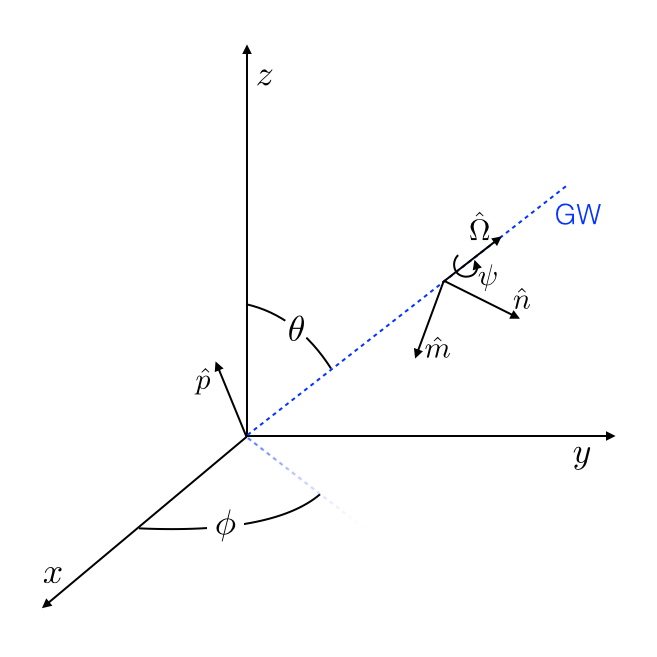
\includegraphics[width=0.8\textwidth]{Img/pulsar_position_diagram_square}
    \bicaption{脉冲星-地球系统。坐标原点选在地球。$\hat{p}$是脉冲星所在的方向。蓝色虚线代表引力波的传播方向。}{The pulsar-Earth system, as visualized with
        the Earth at the origin. The pulsar locates along $\hat{p}$ direction. The gravitational wave propagates as the
        blue dashed line.}
    \label{position_diagram}
\end{figure}
%%%%%%%%%%%%%%%%%%%%%%%%%

引力波引起的脉冲信号的红移不仅取决于脉冲星和地球系统的几何位置关系,还取决于引力波对应的度规扰动\cite{Detweiler:1979wn}。对于位于单位矢量$\hat{p}$方向(即从地球到脉冲的方向)的脉冲星,以及沿$\hat{\Omega}$方向传播的引力波(见\Fig{position_diagram}),脉冲信号的红移和度规扰动的改变成正比,即\cite{Detweiler:1979wn}
%
\beq
z(t,\hat{\Omega}) = 
\frac{1}{2}
\frac{\hat{p}^i\hat{p}^j}{1+\hat{\Omega}\cdot\hat{p}}\Delta h_{ij},
\label{tdredshift}
\eeq
其中
\beq
\Delta h_{ij}
\equiv
h_{ij}(t_{\rm e},\hat{\Omega}) - 
h_{ij}(t_{\rm p},\hat{\Omega}).
\label{delhdef}
\eeq 
上式的$t_{\rm p}$和$t_{\rm e}$分别表示脉冲信号发射的时刻和到达地球的时刻。通过对\Eq{tdredshift}的角度沿天空所有方向进行积分,可以得到总的红移
\beq
z(t) = \int_{S^2} d\hat{\Omega} \, z(t,\hat{\Omega}).
\label{zftot}
\eeq
在脉冲星探测时,我们观测到的并不是红移,而是脉冲信号的计时残差(timing residual),其为红移的积分,即
\beq
r(t) = \int_0^{t} dt' \, z(t').
\label{residual}
\eeq

我们将度规扰动用平面波展开为\cite{Allen:1997ad}
\beq
h_{ij}(t,\vec{x}) = \sum_{A}
\int_{-\infty}^{\infty}df\, \int_{S^2}d\hat{\Omega}\, 
e^{i2\pi f(t-\hat{\Omega}\cdot\vec{x})}
h_A(f,\hat{\Omega})e_{ij}^A(\hat{\Omega}),
\label{pwexp}
\eeq
其中$f$是引力波的频率,$A = +, \times$表示引力波的极化,而$e_{ij}^A(\hat{\Omega})$为引力波的极化张量。利用上式的平面波分解,我们可以得到频率空间的计时残差为%
\e
    \tilde{r}(f,\hat{\Omega}) 
    = \frac{1}{2 \pi i f}\left(1-e^{-2\pi i f L(1+\hat{\Omega}\cdot\hat{p})}\right) 
    \sum_{A} h_A(f,\hat{\Omega}) \left ( e^A_{ij}(\hat{\Omega})
    \frac{\hat{p}^i\hat{p}^j}{2(1+\hat{\Omega}\cdot\hat{p})}\right),
    \label{fdredshift}
\q
其中$L$为脉冲星和地球的距离。极化张量的表达式为
\begin{subequations}
    \begin{align}
        \label{e_plus}
        e_{ij}^+({\hat{\Omega}}) &=  {\hat{m}}_i {\hat{m}}_j - {\hat{n}}_i {\hat{n}}_j,\\
        \label{e_cross}
        e_{ij}^{\times}({\hat{\Omega}}) &= {\hat{m}}_i {\hat{n}}_j + {\hat{n}}_i {\hat{m}}_j.
    \end{align}
\end{subequations}
\Fig{position_diagram}的各个方向为
\begin{subequations}
    \begin{align}
        \label{omega}
        {\hat{\Omega}}&= (\sin{\theta} \cos{\phi},  \sin{\theta} \sin{\phi},  
        \cos{\theta})=\hat r, \\
        \label{m}
        {\hat{m}}&=(\sin{\phi}, -\cos{\phi}, 0)=-\hat\phi, \\
        \label{n}
        {\hat{n}}&=(\cos{\theta}\cos{\phi}, \cos{\theta}\sin{\phi}, -\sin{\theta})=\hat\theta.
    \end{align}
\end{subequations}
假定随机引力波背景是各向同性的、无极化的和稳态的,应变的关联函数为\cite{Detweiler:1979wn}
\e
    \langle h_A^*(f,\hat{\Omega})h_{A'}(f',\hat{\Omega}')\rangle 
    =\frac{3H_0^2}{32\pi^3}\delta^2(\hat{\Omega},\hat{\Omega}')\delta_{AA'}
    \delta(f-f')
    |f|^{-3}\Omega_{\rm GW}(|f|).
    \label{hevom}
\q
所以脉冲星计时残差之间的关联为
\beq\label{e:rexpect}
\langle\tilde{r}_I^*(f)\tilde{r}_J(f')\rangle
= \frac{H_0^2}{16 \pi^4} \delta(f-f')|f|^{-5}
\Omega_{\rm GW}(|f|) \Gamma_{IJ},
\eeq
其中$\Gamma_{IJ}$是脉冲星$I$和脉冲星$J$之间的关联函数(即Hellings \& Downs关联系数)\cite{Hellings:1983fr}
\e\label{hd}
\Gamma_{IJ}=\frac{3}{2} \left[ \frac{1}{3} +
\frac{1-\cos\zeta_{IJ}}{2}\left[ \ln\lp\frac{1-\cos\zeta_{IJ}}{2}\rp
- \frac{1}{6} \right] \right] +\frac{1}{2}\delta_{IJ}.
\q 
上式的$\zeta_{IJ}$是脉冲星$I$和脉冲星$J$之间的角度。脉冲星计时阵列探测随机引力波背景的关键目标就是探测到\Eq{e:rexpect}所对应的关联。
\chapter{原初双黑洞并合率}\label{chap:mergerrate}

\section{背景介绍}

%Up to now several gravitational-wave events from the coalescences of black hole binaries have been reported by LIGO/VIRGO, and imply that black holes should have an extended mass function. We work out the merger rate distribution of primordial-black-hole binaries with a general mass function by taking into account the torques by all primordial black holes and linear density perturbations. In the future, many more coalescences of black hole binaries are expected to be detected, and the one-dimensional and two-dimensional merger rate distributions will be crucial for reconstructing the mass function of primordial black holes. 

人们普遍认为在宇宙早期,由于密度涨落的塌缩,有可能形成原初黑洞\cite{Hawking:1971ei,Carr:1974nx,Carr:1975qj}。另外,理解暗物质的本性到底是什么,依然是困扰物理学界的一大难题。作为暗物质的候选者之一,原初黑洞近年来吸引了越来越多的关注。这是因为原初黑洞不仅可能构成部分或全部的暗物质,而且LIGO-Virgo科学组织探测到的引力波事件\cite{Abbott:2016blz}可能就来源于原初双黑洞的并合\cite{Sasaki:2016jop,Bird:2016dcv}。

根据LIGO-Virgo科学组织最新发布的引力波瞬变目录2\cite{Abbott:2020niy},目前一共探测到了50个致密双星并合事例。其中大多数都是双黑洞并合的事例。引力波的观测表明,黑洞应当有质量分布,而不是单一质量的。事实上,形成原初黑洞的初始条件也表明原初黑洞的质量谱应当有一定的宽度。

在文献中,主要有两种原初黑洞的形成机制。在第一种机制中,原初双黑洞形成于早期宇宙 \cite{Sasaki:2016jop,Nakamura:1997sm,Ali-Haimoud:2017rtz};而在另一种机制中,原初双黑洞形成于晚期宇宙 \cite{Bird:2016dcv,Ali-Haimoud:2017rtz,Nishikawa:2017chy}。研究表明,原初双黑洞的并合率主要由第一种机制主导。在过去的研究中,人们通常假定所有原初黑洞的质量都是一样的,即假定原初黑洞的质量谱是单色的\cite{Sasaki:2016jop,Nakamura:1997sm,Ali-Haimoud:2017rtz,Bird:2016dcv,Nishikawa:2017chy}。最近,文献\cite{Raidal:2017mfl}和文献\cite{Kocsis:2017yty}计算了有质量分布的原初黑洞的并合率。但他们的计算都有可以改进的地方。例如,文献\cite{Raidal:2017mfl}只考虑了距离原初双黑洞系统最近的第三个黑洞对双黑洞系统的潮汐作用,而忽略了其他黑洞对双黑洞系统的相互作用;文献\cite{Kocsis:2017yty}只考虑了平的原初黑洞质量谱,而且质量谱的宽度很窄。

在这一章中,我们将计算最一般质量谱下的原初双黑洞的并合率。在计算过程中,我们将考虑所有其他原初黑洞以及线性物质密度扰动对原初双黑洞系统产生的力矩。在未来的几十年内,我们将探测到越来越多的双黑洞并合事件。进而我们将获取更多的黑洞质量分布的信息。利用黑洞质量分布的信息以及理论模型推演出来的并合率,我们将有可能回答引力波探测到的黑洞的起源以及这些黑洞是如何演化的。

\section{有质量分布情况下的原初双黑洞并合率的计算}
我们将原初黑洞的质量分布函数记作$P(m)$,其满足归一化条件
\e
\int_0^\infty P(m)dm=1.
\q
同时,在质量区间$(m, m+dm)$内的原初黑洞占冷暗物质的丰度为
\e
f_\mathrm{tol} P(m)dm, 
\q
其中$f_\mathrm{tol}$是原初黑洞占非相对论物质的总丰度。为了方便,我们以太阳质量$M_\odot$作为原初黑洞质量的单位。原初黑洞占冷暗物质的丰度和$f_\mathrm{tol}$的关系为$\fpbh\equiv \Omega_{\rm{PBH}}/\Omega_{\rm{CDM}} \approx f_\mathrm{tol}/0.85$。为了方便,我们将质量分布函数做离散化,即
\e
\int P(m)dm=1\ \rightarrow \ \sum_{m_{\rm{min}}\leq m_i \leq m_{\rm{max}}} P_i \Dt \simeq 1, 
\q
其中$P(m_i) \rightarrow P_i$是粗粒化的质量分布函数,而$dm_i \rightarrow \Dt$是原初黑洞质量的微小单元。简单来说,质量为$m_i$的原初黑洞的丰度即为$f P_i \Dt\equiv f_i \Dt$。在物质-辐射平衡时期,总的能量密度为
\e
\rhoeq =\Omega_m \rho_{\rm{crit}} (1+z_{\rm{eq}})^3, 
\q
而两个质量为$m_i$的原初黑洞之间的平均距离$\xbar_i$为
\e
\xbar_i = \({3\over 4\pi} {m_i\over \rhoeq f_i \Dt}\)^{1/3}.
\q
需要注意的是,$\xbar_i$不仅取决于原初黑洞的质量$m_i$,而且取决于该质量的原初黑洞的丰度$f_i \Dt$。需要强调的是不同质量的原初黑洞的数密度可以极不相同的。所以对所有原初黑洞来说,并没有良好定义的数密度概念。对于两个邻近但质量不同的原初黑洞,假定其质量分别为$m_i$和$m_j$,则它们的平均距离为
\e
\langle x_{ij}\rangle=  \(\xbar_i^{-3}+\xbar_j^{-3}\)^{-1/3}
= \mu_{ij}^{1/3} \xbar_{ij}, 
\q
其中 
\m
\mu_{ij}&=& {2m_im_j f_{b}\over m_{b}(f_jm_i+f_im_j)},\label{mu}\\
\xbar_{ij}^3&=&{3\over 8\pi} {m_{b}\over \rhoeq f_{b} \Dt}, %\equiv {{\tilde x}_{ij}^3\over \Dt}, 
\label{xbar}
\n
并且 
\m
f_{b}&=&f_i+f_j,\\
m_{b}&=&m_i+m_j. 
\n 
需要注意的是,以上公式只有当两个原初黑洞具有不同质量,即$m_i\neq m_j$时才成立。当$m_i=m_j=m$时,需要做如下替换$P(m_i)=P(m_j)=P(m)/2$。 
在本章中,在不会混淆的情况下,我们去掉下标`$_{ij}$'。

下面我们考虑原初双黑洞的形成和演化过程。在宇宙早期,两个邻近的原初黑洞需要从宇宙膨胀的背景中退耦出来才能形成双黑洞束缚系统。假设质量为$m_i$和$m_j$的两个原初黑洞沿着运动方向的固有距离为$r$,则在在牛顿近似下,$r$需要满足以下运动方程
\e\label{eom1}
\ddot{r} - \( \dot{H} + H^2 \) r + \frac{m_b}{r^2} \frac{r}{|r|} = 0, 
\q
其中一点表示对固有时间的导数。在本章中,我们使用几何单位制,即要求牛顿常数$G$和光速$c$满足$G=c=1$。

假设两个原初黑洞的共动距离为$x$。为了方便,我们定义$\chi \equiv r/x$。则公式\eqref{eom1}可以改写为
\e
\chi'' + \frac{s h' + h}{s^2 h} \(s \chi' - \chi \) + \frac{1}{\la}
\frac{1}{\(sh\)^2} \frac{1}{\chi^2} \frac{\chi}{|\chi|} = 0, 
\label{chi}
\q
其中一撇代表对尺度因子$s$的导数。我们将尺度因子在物质-辐射平衡时期的大小定为1。公式\eqref{chi}的$h(s)$定义为$h(s)\equiv H(s)/\({8\pi\over 3}\rhoeq\)^{1/2}=\sqrt{s^{-3}+s^{-4}}$。这里的$\la$是一个无量纲的参数,其定义为
\e
\la = \frac{8 \pi \rhoeq x^3}{3 m_b} = {X\over f_b\Dt},
\q
其中
\e
X\equiv {x^3/\xbar^3}, 
\q
其中$\xbar$由公式\eqref{xbar}给出。由公式\eqref{chi}的解可以看出如果$\lambda<1$则退耦会发生在物质-辐射平衡之前\cite{Ali-Haimoud:2017rtz}。另外,双黑洞系统的半长轴$a$的解为
\e
a \approx 0.1 \la x = \frac{0.1}{f_b \Dt} \frac{x^4}{\xbar^3}
={0.1 \xbar \over f_b\Dt} X^{\frac{4}{3}}. 
\label{axis}
\q 

如果没有其他黑洞或者密度扰动提供潮汐力,双黑洞则会直接迎头碰撞而并合。如果有潮汐力的话,那么潮汐力会为双黑洞系统提供角动量,从而使得双黑洞形成束缚系统,而不是直接并合。为了方便,我们引入一个无量纲的角动量$j$,其定义为 
\e
j\equiv \ell/\sqrt{m_b a}=\sqrt{1-e^2}, 
\q
其中$\ell$为单位约化质量的角动量。另外$e\in[0,1]$为偏心率。下面的关键问题乃是估计初始轨道的参数。我们推广了文献\cite{Ali-Haimoud:2017rtz}中的方法来估算两个具有不同质量的原初黑洞构成的双黑洞系统的初始轨道参数。下面我们给出简要的推导过程。

假设牛顿势为$\phi$,则局域的潮汐场为$T_{ij}=-\p_i\p_j \phi$。潮汐场会产生潮汐力。对每单位质量,潮汐力的大小为$\mathbf{F}=\mathbf{T}\cdot \mathbf{r}$。由于双黑洞系统的初始共动距离要比平均距离小很多,所以潮汐力并不会对双黑洞的轨道有很大的影响。潮汐力会产生力矩,其大小为
\e
\mathbf{\ell}=\int dt\ \mathbf{r}\times [\mathbf{T}\cdot \mathbf{r}]. 
\q
由于在辐射主导时期,其他原初黑洞以及密度涨落产生的潮汐场正比于$s^{-3}$,即$\mathbf{T}\simeq s^{-3} \mathbf{T}_{\rm{eq}}$,所以角动量为
\e\label{angular_j}
\bj \approx x^3 \hx \times \[\frac{\mathbf{T}_{\rm{eq}}}{m_b} \cdot \hx \], 
\q
其中$\hx$是沿着$\mathbf{x}$方向的单位矢量,而$\mathbf{T}_{\rm{eq}}$是在物质-辐射平衡时期的局域潮汐场。现在考虑质量为$m_l$的第三个原初黑洞。假设这个黑洞与双黑洞的距离$y$远远大于双黑洞的距离$x$,即$y\gg x$,则第三个黑洞产生的潮汐场为
\e
T^{ij}_{eq} = m_l \frac{3 \hy^i \hy^j - \dt^{ij}}{y^3},
\q
其中$\hy$是沿着$\mathbf{y}$方向的单位矢量。\eqref{angular_j}式进而可以变为
\e
\mathbf{j} \approx 3 \frac{m_l}{m_b} \frac{x^3}{y^3} 
\(\hx \cdot \hy\) \(\hx \times \hy\).
\q
与文献\cite{Ali-Haimoud:2017rtz}类似,下面我们参照\cite{Chandrasekhar:1943ws}来计算角动量的概率分布函数。所有其他黑洞产生的角动量$j$的二维概率密度函数为
\e
\frac{dP}{d^2 j} = \lim_{V \to \infty}\int \frac{d^2 k}{\(2\pi\)^2} e^{i \mathbf{k} \cdot \bj} 
\prod_{l} {\cal I}_l^{N_l},
\q
其中$N_l=n_l V$是所有质量为$m_l$的原初黑洞的数目。另外,${\cal I}_l$为
\e
{\cal I}_l = \int_V \frac{d^3 y}{V} \exp\[-3 \frac{m_l}{m_b} i
\frac{x^3}{y^5} y_{||}\, \mathbf{k} \cdot \mathbf{y}_{\perp}\],
\q
其中$y_{||}$和$\mathbf{y}_{\perp}$分布定义为$y_{||}\equiv \mathbf{y}\cdot \hx$, $\mathbf{y}_{\perp}\equiv \hx\times \mathbf{y}$。经过繁琐的计算,我们会得到
\m
\lim_{V \to \infty} {\cal I}_l^{N_l} = e^{-{4\pi\over 3} {m_l\over m_b} n_l x^3 k}. 
\n
由于所有质量为$m_l$的原初黑洞的能量密度为$m_l n_l=\rho_l$,并且$\sum_l \rho_l=\rho_{\rm{pbh}}=f \rhoeq$,所以我们可以得到
\m\label{prob1}
\frac{dP}{dj} = j \int k dk J_0(kj) e^{-j_X k},
\n 
其中
\m
j_X=0.5{f\over f_b\Dt} X.
\n
$j_X$表征了所有其他原初黑洞产生的力矩的总和。对公式\eqref{prob1}积分会得到
\m\label{Pj}
\left. j \frac{dP}{dj} \right\vert_X = \mP\(j/j_X\), \quad
\mP(\ga) = \frac{\ga^2}{\(1 + \ga^2\)^{3/2}},
\label{pj}
\n
其中$\gamma=j/j_X$。此外,密度涨落产生的力矩$\mathbf{j}$的方差为
\e
\langle j^2 \rangle^{1/2}\approx 0.5 {8\pi\over 3} {\sigma_{\rm{eq}}\rhoeq \over m_b}x^3=0.5 {\sigma_{\rm{eq}}\over f_b\Dt} X, 
\q
其中$\sigma_{\rm{eq}}\equiv \langle \delta_{\rm{eq}}^2 \rangle^{1/2}$是其他暗物质在物质-辐射平衡时期在${\cal O}(10^0\sim10^3) M_\odot$尺度上的密度涨落的方差。考虑到所有其他原初黑洞以及密度涨落产生的力矩,那么\eqref{pj}式中的$j_X$的特征大小为 
\e
j_X\approx 0.5 \(f^2+\sigma_{\rm{eq}}^2\)^{1/2} {X\over f_b\Dt}. 
\label{jx}
\q

在形成原初双黑洞系统后,由于引力波辐射,双黑洞系统的轨道会收缩,最后并合。双黑洞的并合时间由系统的质量、轨道距离以及角动量共同决定,具体为\cite{Peters:1964zz}
\m 
t = \frac{3}{85} \frac{a^4}{m_i m_j m_b} j^7.
\n 
考虑到公式\eqref{axis},则无量纲的的角动量为
\m 
j(t; X) = \( \frac{85}{3} \frac{t m_i m_j m_b (f_b\Dt)^4}
{\(0.1\xbar\)^4 X^{16/3}} \)^{1/7}.
\n  
假设所有原初黑洞在空间上是随机分布的,则两个为$m_i$和$m_j$的最相邻原初黑洞的距离为$x$,且在体积${4\pi \over 3}x^3$内没有其他原初黑洞的概率为
\m 
% \frac{dP}{d{\tilde X}} = e^{- {\tilde X}},
\frac{dP}{d{\tilde X}} = e^{- {4\pi \over 3}x^3 n_T}=e^{- {\tilde X}\cdot {4\pi \over 3}\langle x_{ij} \rangle^3 n_T}, 
\label{dpX}
\n 
其中${\tilde X}\equiv x^3/\langle x_{ij} \rangle^3=X/\mu$,而$\mu$由公式\eqref{mu}给出,并且$n_T\equiv f\rho_{\rm{eq}}\int_0^\infty {P(m)\over m}dm$。如果$m_i\approx m_j$,则$\mu\approx 1$。但是如果两个原初黑洞的质量比很大的话,那么$\mu$可以远远小于$1$,那么文献\cite{Ali-Haimoud:2017rtz}中给出的近似表达式$dP/dX\approx 1$ 将不再有效。需要注意的是,我们推广了文献\cite{Ali-Haimoud:2017rtz}计算单一质量原初黑洞的结果,我们发现在有质量分布的情况下,在指数项会有一个$1/\mu$因子的修正。在$m_i = m_j$的特例下,$\mu = 1$,进而我们的结果退回到文献\cite{Ali-Haimoud:2017rtz}的结果。然而,对于极端质量比的双黑洞系统,这个因子可能会产生很大影响,进而导致文献\cite{Ali-Haimoud:2017rtz}使用的近似表达是$e^{- X/\mu} \app 1$不再有效。利用关系式$j \propto t^{1/7}$,$\p j/\p t = j/(7t)$和公式\eqref{Pj},我们得到
\e
\frac{d^2 P}{d{\tilde X} dt} = \frac{1}{7 t} e^{- {\tilde X}\cdot {4\pi \over 3}\langle x_{ij} \rangle^3 n_T}\, \mP(\ga_X),
\quad \ga_X \equiv \frac{j(t; X)}{j_X}, 
\q 
其中$j_X$由公式\eqref{jx}给出。对上式的$\tilde{X}$进行积分,我们可以到并合时间的概率分布函数
\e 
\frac{dP}{dt}  %\int \frac{d{\tilde X}}{7 t}  e^{- {\tilde X}\cdot {4\pi \over 3}\langle x_{ij} \rangle^3 n_T} \mP(\ga_X) \nonumber\\
= \frac{\mu^{-1}}{7 t} \int d{X} e^{- {X\over \mu}\cdot {4\pi \over 3}\langle x_{ij} \rangle^3 n_T} \mP(\ga_X),
\label{dP}
\q
进而在时间$t$时,原初黑洞的共动并合率为
\m
R_{ij}(t)\equiv {dN_{\rm{merger}}\over dtdV}=\rho_m^0 \min\(\frac{f_i \Dt}{m_i}, \frac{f_j \Dt}{m_j}\) {dP\over dt}, 
\n
其中$\rho_m^0\simeq 4\times 10^{19}\, \Msun \text{Gpc}^{-3}$为今天的物质密度。概率函数${\cal P}(\gamma_X)$有一个很尖的峰,其尖峰的位置为
\e
X_*(t)\approx 0.032 \({t\over t_0}\)^{3\over 37} f_b \Delta (f^2+\sigma_{\rm{eq}}^2)^{-{21\over 74}} (m_i m_j)^{3\over 37} m_b^{-{1\over 37}}.
\q
由于${X_*\over \mu}\cdot {4\pi \over 3}\langle x_{ij} \rangle^3 n_T\ll 1$, 所以在$t$时刻的共动并合率为
\m
R_{ij}(t)= {\cal R}_{ij}(t) \Delta^2, 
\n
其中  
\m
{\cal R}_{ij}(t)&\approx& 3.9\cdot 10^6\times  \({t\over t_0}\)^{-{34\over 37}} f^2 (f^2+\sigma_{\rm{eq}}^2)^{-{21\over 74}} \nonumber \\
&\times&  \min\(\frac{P(m_i)}{m_i}, \frac{P(m_j)}{m_j}\) \({P(m_i)\over m_i}+{P(m_j)\over m_j}\) \nonumber \\
&\times& (m_i m_j)^{{3\over 37}} (m_i+m_j)^{36\over 37}.
\n
${\cal R}_{ij}(t)$是以Gpc$^{-3}$ yr$^{-1}$为单位的共动并合率密度分布。需要注意到是,本章中原初黑洞的质量是以太阳质量$M_\odot$为单位的。需要再次强调的是,在$m_i=m_j=m$时,$P(m_i)=P(m_j)=P(m)/2$。文献\cite{Kocsis:2017yty}定义了一个量$\tilde{\alpha} \equiv -(m_i+m_j)^2\p^2 \ln {\cal R}_{ij}/\p m_i \p m_j$,且认为$\tilde{\alpha}$的值应该约等于$36/37$。如果$P(m)/m=$是个常数的话,那么$\tilde{\alpha}=36/37$,则和文献\cite{Kocsis:2017yty}的结果吻合。但是对于一个一般的质量函数分布,$\tilde{\alpha}$可以不同于$36/37$。

\section{与引力波数据的比较}
下面我们考虑文献中经常用到的2个原初黑洞的质量函数分布。第一个是幂率分布\cite{Carr:1975qj}
\m
P(m)\approx {\alpha-1\over M} \({m\over M}\)^{-\alpha}
\n
其中$m\geq M$,且$\alpha>1$。第二个为对数正态分布\cite{Dolgov:1992pu}
\m
P(m) = \frac{1}{\sqrt{2 \pi} \sigma m} 
\exp\(-\frac{\ln^2(m/m_c)}{2 \sigma^2}\), 
\n
其中$m_c$表征质量谱的峰值,而$\s$表征质量谱的宽度。
在文献\cite{Abbott:2017vtc}中,LIGO-Virgo科学组织限制了质量范围在$m_1,\ m_2\geq 5M_\odot$和 $m_1+m_2\leq 100M_\odot$内的双黑洞的并合率大小$R_T$,要求$12 \lesssim R_T \lesssim 213$ Gpc$^{-3}$ yr$^{-1}$。与文献\cite{Ali-Haimoud:2017rtz}一样,我们取$\sigma_{\rm{eq}}\approx 0.005$。在图\ref{merger}我们列出了这两种质量分布下的并合率随着原初黑洞丰度的关系。其中粉红色区域是LIGO-Virgo科学组织给出的并合率的范围。在这个图中,对于幂率质量分布函数,我们选取$M=5\Msun$和$\alpha=1.6$;而对于对数正态质量分布函数,我们选取$m_c=15M_\odot$和$\sigma=0.6$。从这个图可以看出,用原初黑洞模型确实可以解释LIGO-Virgo科学组织探测的双黑洞。
从LIGO-Virgo科学组织给出的并合率限制,我们可以反推出原初黑洞占暗物质丰度$\fpbh$的限制。对于幂率形式的质量分布函数,$\fpbh$需要满足$1.4\times 10^{-3} \lesssim \fpbh \lesssim 6.6\times 10^{-3}$;而对于对数正态形式的质量分布函数,$\fpbh$需要满足$1.2\times 10^{-3} \lesssim \fpbh \lesssim 5.7\times 10^{-3}$。以上得到的$\fpbh$的限制和其他观测\cite{Chen:2016pud,Green:2016xgy,Schutz:2016khr,Wang:2016ana,Gaggero:2016dpq,Ali-Haimoud:2016mbv,Blum:2016cjs,Horowitz:2016lib,Kuhnel:2017pwq,Inoue:2017csr,Carr:2017jsz,Green:2017qoa,Guo:2017njn,Zumalacarregui:2017qqd,Clesse:2016vqa}给出来的是一致的。

\begin{figure}[htb]
    \centering
    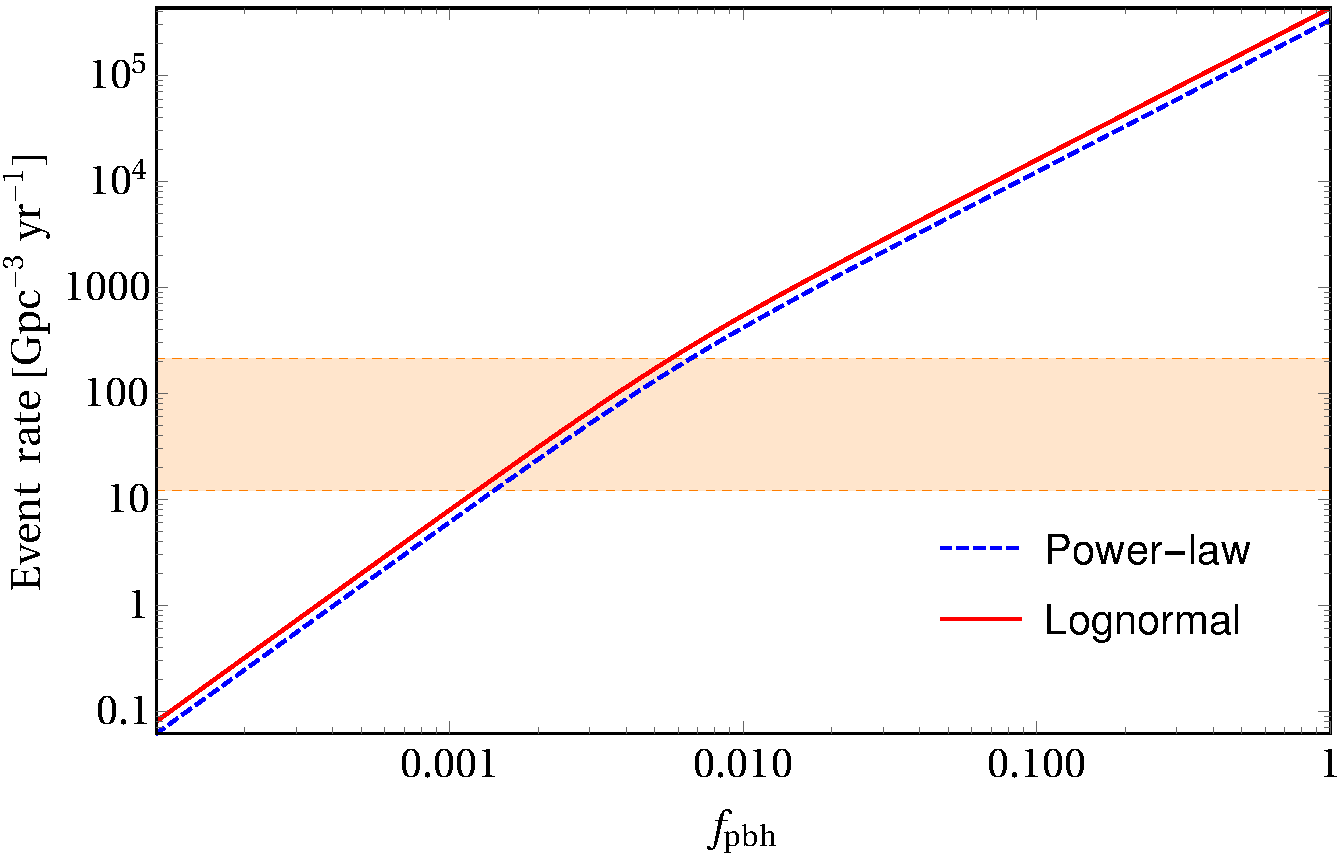
\includegraphics[width=0.86\textwidth]{mergerfpbh.pdf}
    \bicaption{ 
        在质量为$m_1,\ m_2\geq 5M_\odot$且$m_1+m_2\leq 100M_\odot$的范围内,今天的原初双黑洞的并合率和$\fpbh$的关系图。蓝色点线和红色实线分别对应为\textit{幂率}质量分布函数($M=5M_\odot$且$\alpha=1.6$)和\textit{对数正态}质量分布函数($m_c=15M_\odot$且 $\sigma=0.6$)。
    }{The merger rate of PBH binaries at present as a function of $\fpbh$ with $m_1,\ m_2\geq 5M_\odot$ and $m_1+m_2\leq 100M_\odot$. The blue dotted and red solid lines correspond to the \textit{power-law} mass distribution ($M=5M_\odot$ and $\alpha=1.6$) and \textit{lognormal} mass distribution ($m_c=15M_\odot$ and $\sigma=0.6$), respectively. }
    \label{merger}
\end{figure}

\begin{figure}[htb!]
    \centering
    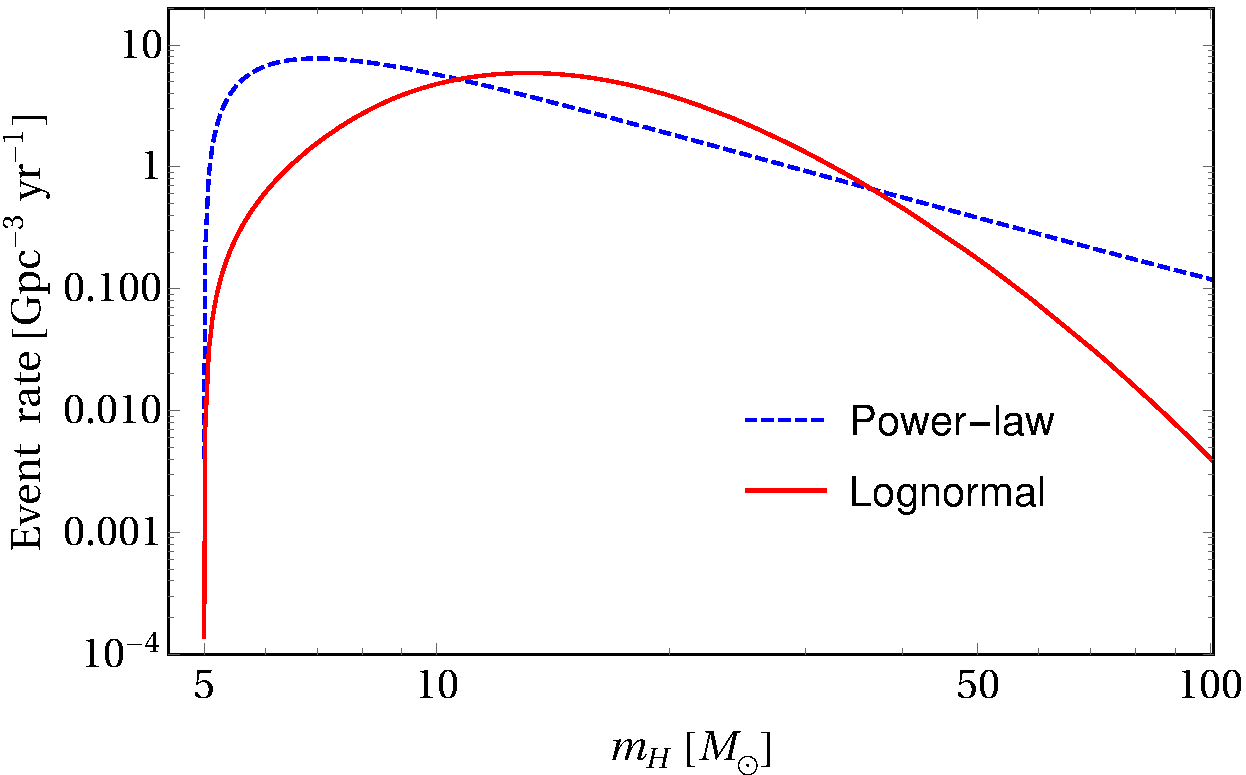
\includegraphics[width=0.86\textwidth]{mergerheavy.pdf}
    \bicaption{\label{mergerheavy}
        一维的并合率分布。其中$m_H$是双黑洞系统中较重黑洞的质量。我们把较轻黑洞的质量积分掉,积分范围为$5M_\odot$到$m_H$。蓝色实线对应的是$\fpbh =4.3\times 10^{-3}$时的\textit{幂率}形式的质量分布函数($M=5M_\odot$且$\alpha=1.6$);而红色实线对应的是$\fpbh = 3.7\times 10^{-3}$时的\textit{对数正态}形式的质量函数分布($m_c=15M_\odot$且$\sigma=0.6$)。
    }{The 1D merger rate distribution, where $m_H$ is the mass of heavier BH in the binary and the mass of lighter BH is integrated over from $5M_\odot$ to $m_H$. The blue dotted and red solid lines correspond to the \textit{power-law} PDF ($M=5M_\odot$ and $\alpha=1.6$) with $\fpbh =4.3\times 10^{-3}$ and \textit{lognormal} PDF ($m_c=15M_\odot$ and $\sigma=0.6$) with $\fpbh = 3.7\times 10^{-3}$, respectively.}
\end{figure}

从图\ref{merger}可以看出,不同的质量分布都能解释目前LIGO-Virgo得到的并合率限制。为了打破这种简并,我们需要更多的信息。假如固定总的并合率为$R_T=100$ Gpc$^{-3}$ yr$^{-1}$,对于幂率形式的质量函数,我们可以得到$\fpbh = 4.3\times 10^{-3}$;而对于对数正态形式的质量分布函数,我们可以得到$\fpbh = 3.7\times 10^{-3}$。在图\ref{mergerheavy}中,通过把较轻的黑洞质量积分掉,我们画出了一维的并合率分布。可以看出,尽管幂率形式的质量分布和对数正态形式的质量函数分布都能给出相同的总并合率$R_T$,然而它们对应的一维并合率分布却大不相同。在图\ref{density}中,我们给出了二维的并合率分布中,由此我们可以得到更多的信息。

为了将计算得到的并合率和LIGO-Virgo探测到的引力波事件作比较,我们需要考虑LIGO-Virgo引力波探测器的灵敏度。这是因为并不是所有发生并合的双黑洞事件都能被LIGO-Virgo探测到,只有那些辐射出来的引力波的频率正好处于LIGO-Virgo灵敏的频段才能被LIGO-Virgo探测到。由于现阶段LIGO-Virgo能够探测到的并合事件的红移$z$大概在$z \in [0,1]$,所以预计能探测到的事件数$\Lambda$大致为\cite{Abbott:2016nhf,Abbott:2016drs,Abbott:2017iws,Kavanagh:2018ggo}
\e\label{lambda}
\Lambda_{ij} = \int_{0}^{1} R_{ij}(z) \frac{d\VT}{dz} dz,
\q 
其中$\VT$是LIGO-Virgo平均能探测到的时空体积。$\VT$不仅取决于探测器本身,而且还取决于双黑洞源的性质,比如双黑洞的质量大小。仿照\cite{Abbott:2016nhf,Abbott:2016drs,Usman:2015kfa,Veitch:2014wba},我们采取半解析的方法来计算$\VT$。在这里,我们假设LIGO的第一个观测阶段(O1)和第二观测阶段(O2)具有相同的空间体积。对于第一个探测阶段,其有$48.6$天的有效观测时间\cite{TheLIGOScientific:2016pea};而对于第二个探测阶段,其有$117$天的有效观测时间\cite{TheLIGOScientific:2017qsa}。需要注意的是,$\Lambda$并不是被探测到的双黑洞并合事件的平均数,而是超过一定阀值的事件数的平均值\cite{Abbott:2016nhf}。在这里我们取信噪比(SNR>8)作为可探测的阀值。在图\ref{events1}中,我们给出了二维的可探测事件数$\Lambda$的分布,以及LIGO-Virgo探测到的$6$个双黑洞并合事件。由于我们只用了有限的$6$个引力波事件,所以并不能最终确定哪个形式的质量分布函数和引力波数据拟合得更好。随着探测到双黑洞并合事件的累积,利用我们计算得到的原初黑洞并合率的分布,我们有可能确定黑洞质量函数的形式,以及黑洞质量到底有没有质量间隙\cite{Kovetz:2016kpi,Fishbach:2017zga}。

\begin{figure}[htb]
    \centering
    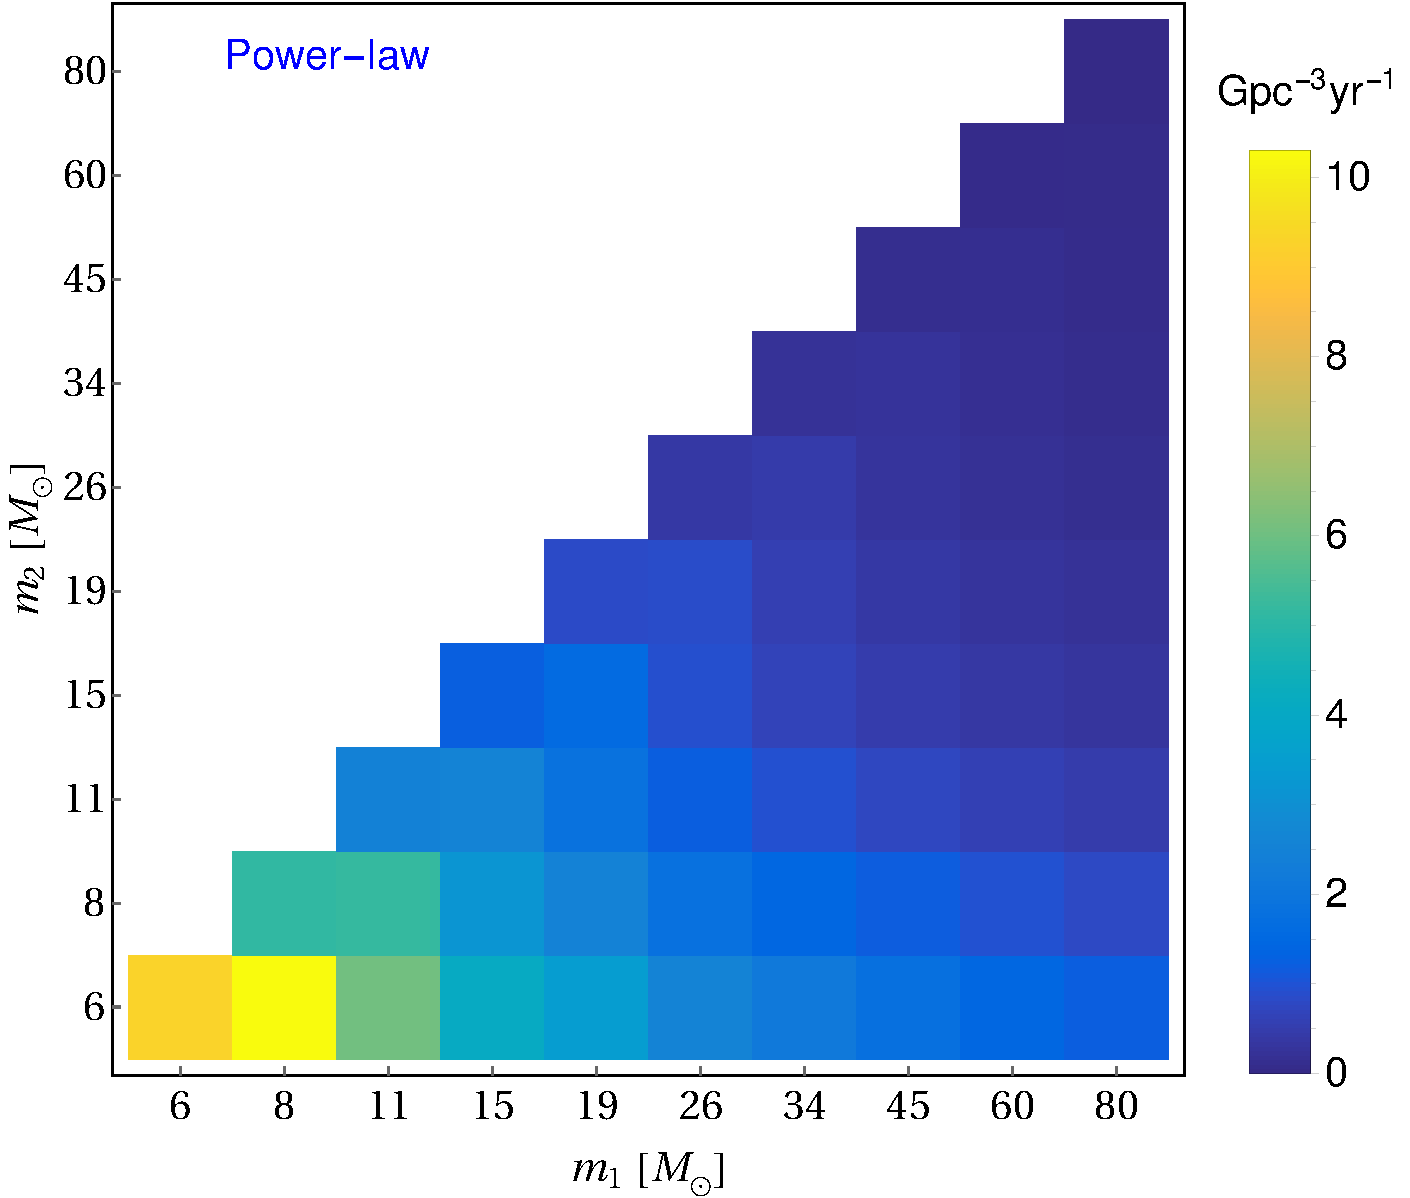
\includegraphics[width=0.8\textwidth]{binpower.pdf}\\
    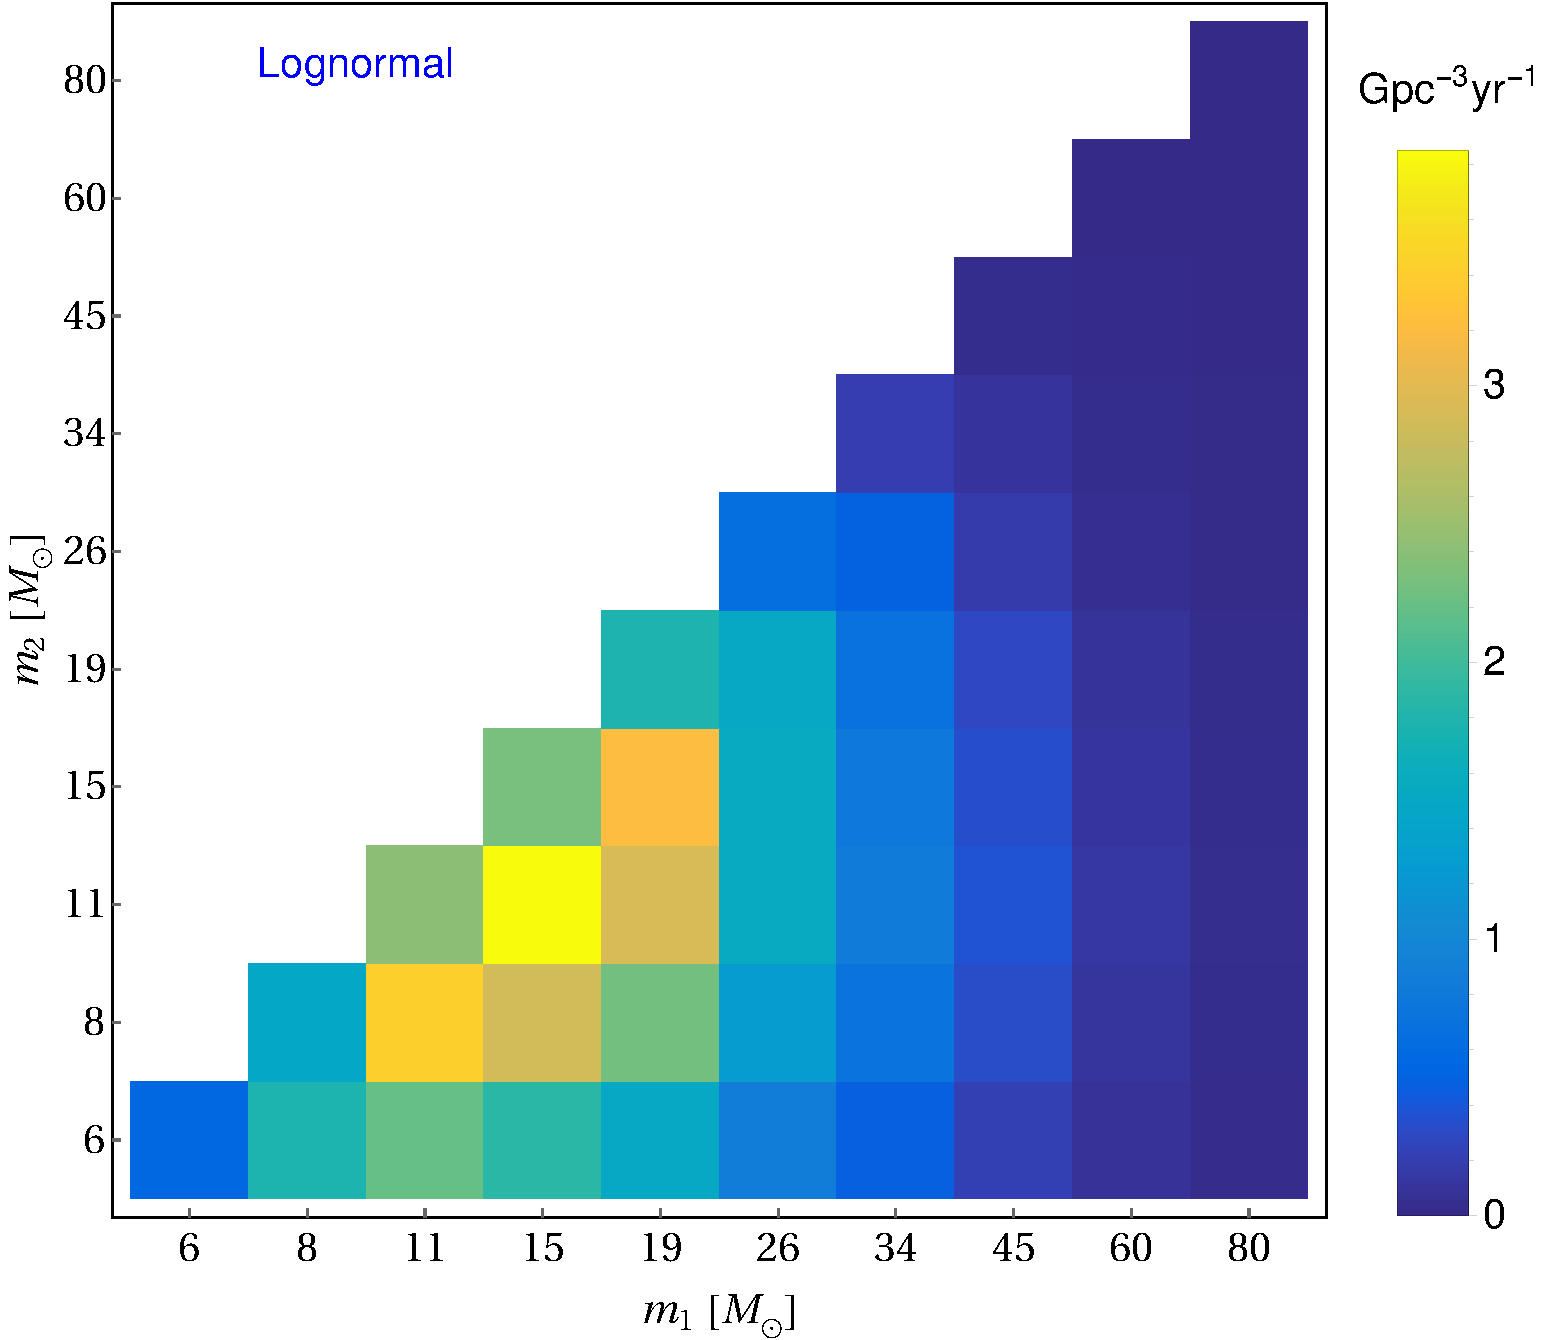
\includegraphics[width=0.8\textwidth]{binlog.pdf}
    \bicaption{\label{density}
        二维的并合率分布。上图对应的是$\fpbh = 4.3\times 10^{-3}$时的\textit{幂率}形式的质量函数($M=5M_\odot$且$\alpha=1.6$);而下图对应的是$\fpbh = 3.7\times 10^{-3}$时的\textit{对数正态}形式的质量函数($m_c=15M_\odot$且$\sigma=0.6$)。
    }{The 2D merger rate distributions. The top and bottom panels correspond to the \textit{power-law} mass function ($M=5M_\odot$ and $\alpha=1.6$) with $\fpbh = 4.3\times 10^{-3}$ and \textit{lognormal} mass function ($m_c=15M_\odot$ and $\sigma=0.6$) with $\fpbh = 3.7\times 10^{-3}$, respectively.}
\end{figure}

\begin{figure}[htb]
    \centering
    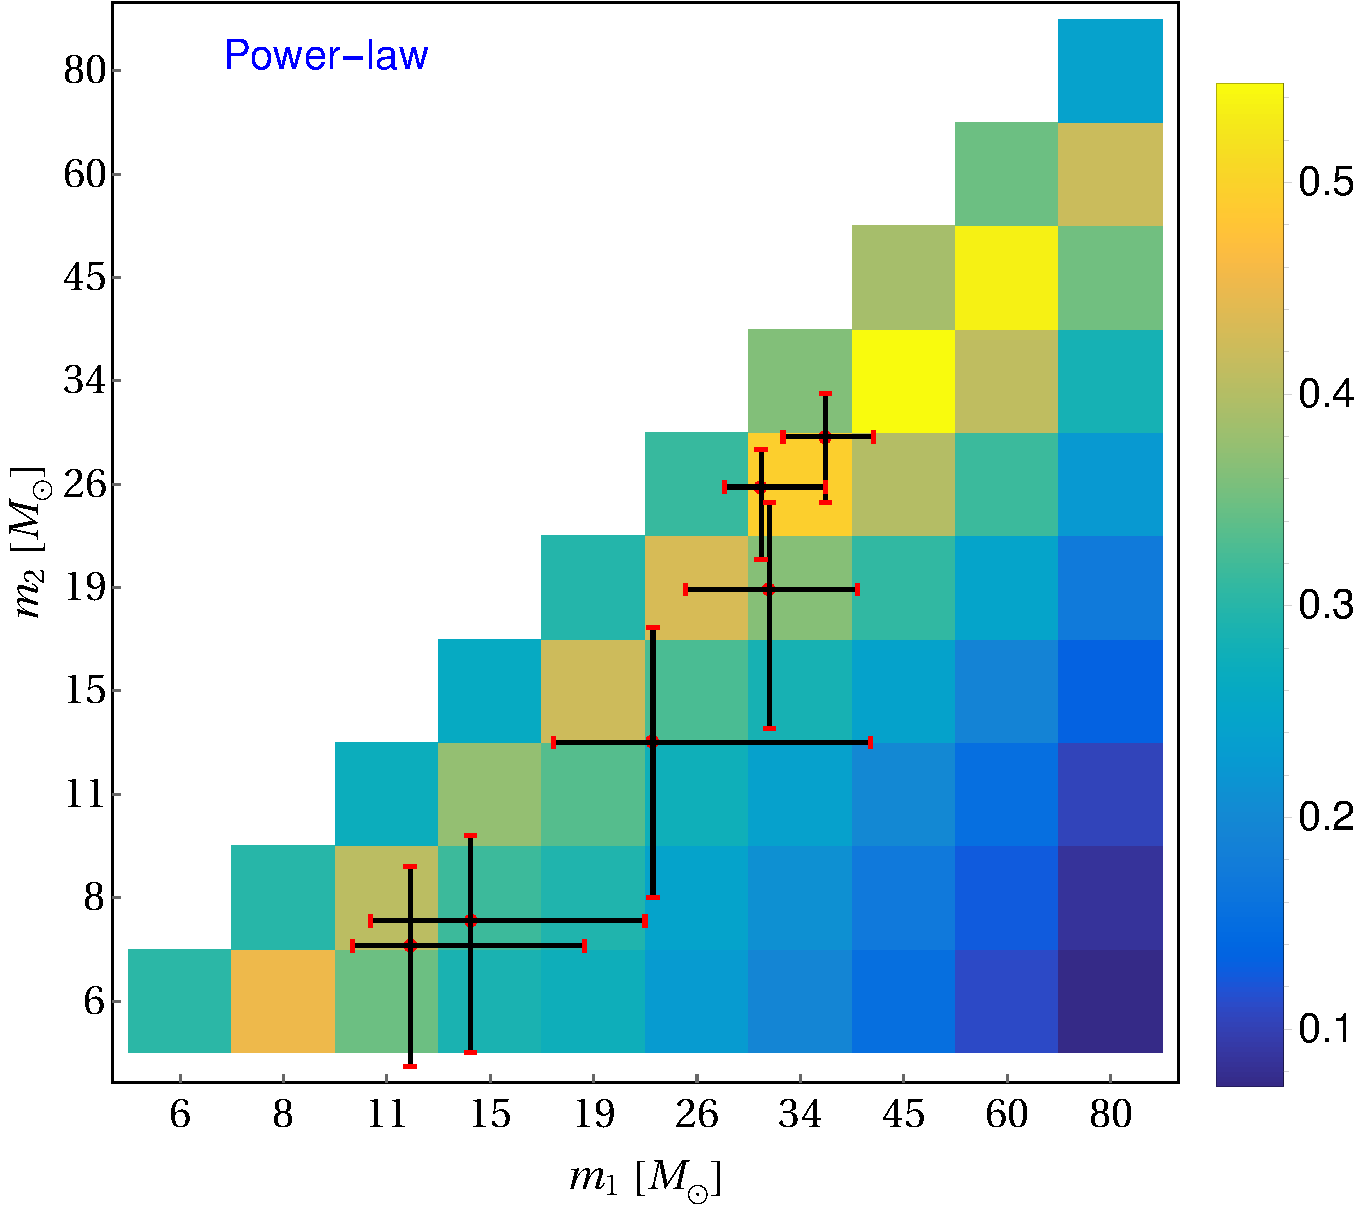
\includegraphics[width=0.72\textwidth]{binpowerrescale.pdf}
    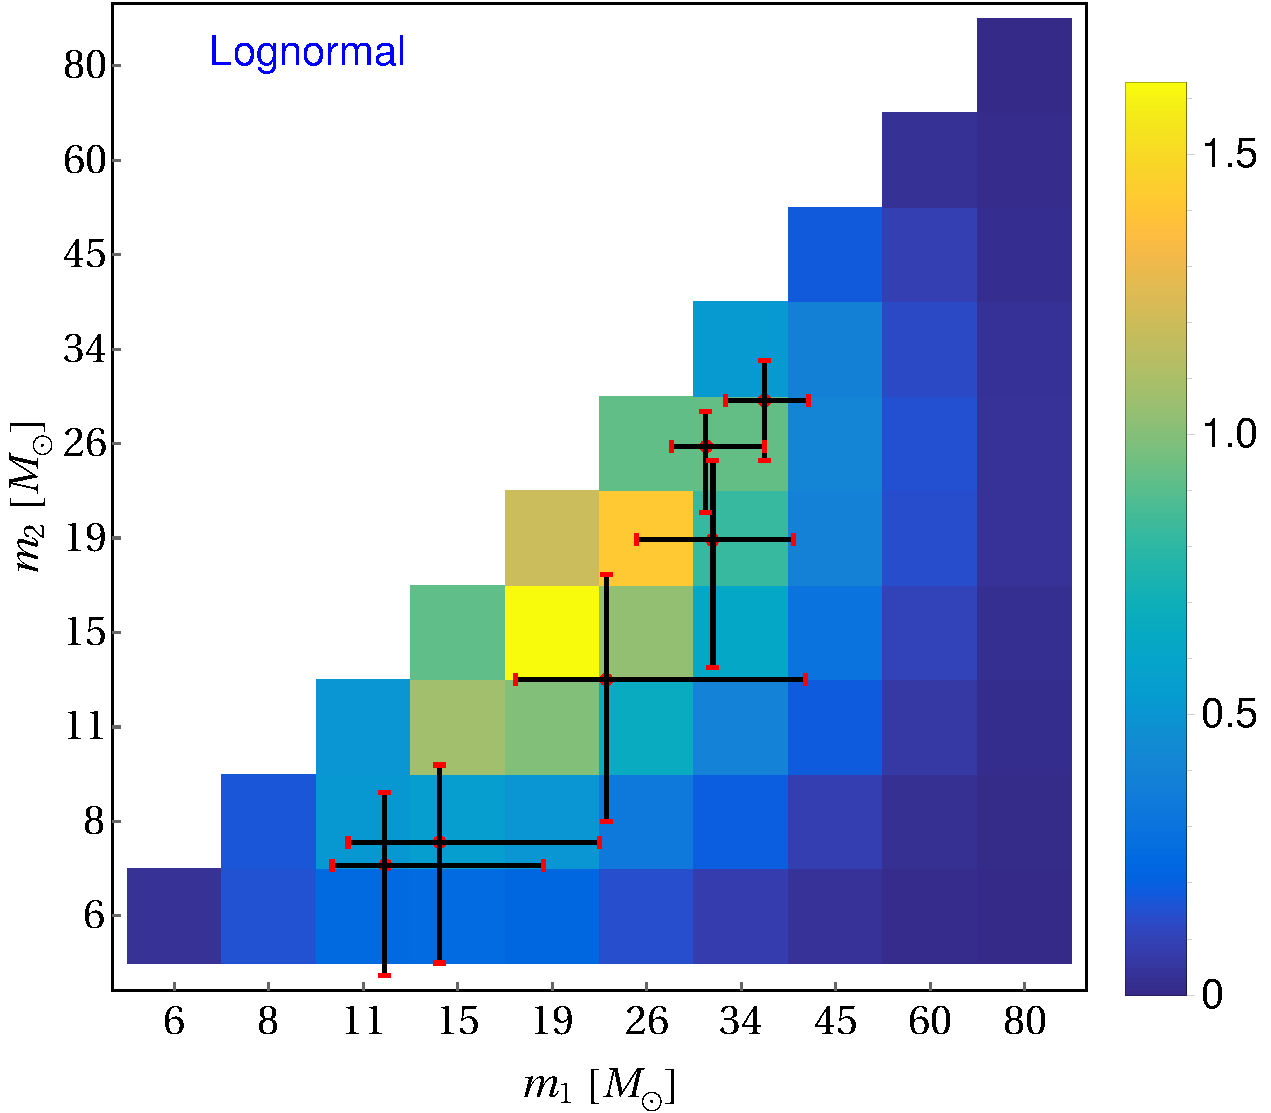
\includegraphics[width=0.72\textwidth]{binlogrescale.pdf}
    \bicaption{\label{events1}
        二维的可探测到的事件数$\Lambda$的分布[见公式\eqref{lambda}],以及LIGO-Virgo探测到的$6$个双黑洞并合事件。每个双黑洞并合事件的质量误差由图中的十字叉给出。上图对应的是$\fpbh = 4.3\times 10^{-3}$时的\textit{幂率}形式的质量函数($M=5M_\odot$且$\alpha=1.6$);而下图对应的是$\fpbh = 3.7\times 10^{-3}$时的\textit{对数正态}形式的质量函数($m_c=15M_\odot$且$\sigma=0.6$)。
    }{The 2D distributions for $\Lambda$ [see Eq.~\eqref{lambda}],
    along with the $6$ events detected by \lvc. 
    The crosses indicate error bars for each event.
    The top and bottom panels correspond to the \textit{power-law} 
    mass function ($M=5M_\odot$ and $\alpha=1.6$) with $\fpbh = 4.3\times 10^{-3}$
    and \textit{lognormal} mass function ($m_c=15M_\odot$ and $\sigma=0.6$) with $\fpbh = 3.7\times 10^{-3}$, respectively. }
\end{figure}

\section{本章小结}
在本章中,我们计算了具有一般质量分布情况下的原初双黑洞的并合率分布。在计算过程中,我们考虑所有其他原初黑洞以及线性密度扰动产生的力矩对原初双黑洞演化的影响。然后我们将计算得到的并合率分布与引力波数据做比较。我们分别考虑了幂率形式以及对数正态形式的原初黑洞的质量函数。对于幂率和对数正态形式的原初黑洞的质量函数,其对应的原初黑洞占暗物质的丰度$\fpbh$大概的量级为$10^{-3} \lesssim \fpbh \lesssim 10^{-2}$。我们得到的结果和其他观测\cite{Chen:2016pud,Green:2016xgy,Schutz:2016khr,Wang:2016ana,Gaggero:2016dpq,Ali-Haimoud:2016mbv,Blum:2016cjs,Horowitz:2016lib,Kuhnel:2017pwq,Inoue:2017csr,Carr:2017jsz,Green:2017qoa,Guo:2017njn,Zumalacarregui:2017qqd,Clesse:2016vqa}给出的结果是一致的,证实了绝大多数的暗物质不是由太阳质量的原初黑洞构成的\cite{Sasaki:2016jop,Ali-Haimoud:2017rtz,Raidal:2017mfl,Kocsis:2017yty}。

目前有很多模型可以解释LIGO-Virgo探测到的双黑洞并合事件。观测这些双黑洞并合率的分布可能是区分原初黑洞模型和其他模型的一种强有力手段。我们发现原初双黑洞的并合率正比于$t^{-34/37}$。这是原初黑洞模型显著区别于其他模型的地方之一。此外,我们还发现一维和二维的并合率分布对原初黑洞的质量分布非常敏感。随着观测时间的增加以及引力波探测器的升级换代,未来我们可以观测到越来越多的双黑洞并合事件。利用一维和二维的原初黑洞并合率分布,我们有望重构出原初黑洞的质量分布,进而帮助我们理解LIGO-Virgo科学组织探测到的黑洞到底是怎么形成的,以及是如何演化的。
\chapter{双黑洞和双中子星并合产生的引力波背景}\label{chap:SGWB}

%The advent of gravitational wave (GW)和multi-messenger astronomy has stimulated the research on the formation mechanisms of binary black holes (BBHs) observed by LIGO/Virgo. In literature, the progenitors of these BBHs could be stellar-origin black holes (sBHs) or primordial black holes (PBHs). In this paper we calculate the Stochastic Gravitational-Wave Background (SGWB) from BBHs, covering the astrophysical和primordial scenarios separately, together with the one from binary neutron stars (双中子星). Our results indicate that PBHs contribute a stronger SGWB than that from sBHs, and the total SGWB from both BBHs和双中子星 has a high possibility to be detected by the future observing runs of  LIGO/Virgo和LISA. On the other hand, the SGWB from BBHs和双中子星 also contributes an additional source of confusion noise to LISA's total noise curve,和then weakens LISA's detection abilities. For instance, the detection of massive black hole binary (MBHB) coalescences is one of the key missions of LISA, and the largest detectable redshift of MBHB mergers can be significantly reduced.


\section{背景介绍}

\lvc 科学组织已经探测到双黑洞和双中子星并合产生的引力波\citep{TheLIGOScientific:2016pea,TheLIGOScientific:2016qqj,Abbott:2016nmj,Abbott:2016blz,    TheLIGOScientific:2017qsa,Abbott:2017vtc,Abbott:2017gyy,Abbott:2017oio},为我们打开一扇探索宇宙的新窗口,并且引领人类进入了引力波天文学和多信使引力波天文学的新时代。截至目前,\lvc 科学组织已经探测到了几十例双黑洞并合的引力波事件。然而这些双黑洞到底是如何产生和演化的,目前还有争议。事实上,在文献中多种不同的形成机制来解释\lvc 探测到的双黑洞并合事件。假设\lvc 探测到的所有黑洞都是来自天体演化形成的,那么恒星级质量的双黑洞的并合率被限制为$12-213\, \gpcyr$ \citep{Abbott:2017vtc}。另外,利用探测到的双中子星并合事件GW170817 \citep{TheLIGOScientific:2017qsa},可以估算双中子星的并合率为$1540\,^{+3200}_{-1220}\, \gpcyr$。

由于地基引力波探测器探测能力的限制,\lvc 引力波探测器目前只能探测到红移$z<1$以内的双黑洞并合产生的引力波事件\citep{TheLIGOScientific:2016htt,Aasi:2013wya}。所以,除了被\lvc 探测到的双黑洞外,宇宙中还有许许多多无法被\lvc 探测到的双黑洞或其他星体并合的事件。这些致密天体并合的过程中产生的引力波会相互叠加形成随机引力波背景\citep{Christensen:1992wi}。不同的双黑洞形成机制预言的双黑洞的并合率和质量及红移的关系通常也不同,所以不同的双黑洞形成机制通常会预言不同的随机引力波背景能量谱。

假设\lvc 探测到的所有的黑洞都来自天体演化形成的\citep{Belczynski:2010tb,Miller:2016krr,TheLIGOScientific:2016htt,Belczynski:2016obo,Stevenson:2017tfq},文献\cite{TheLIGOScientific:2016wyq,TheLIGOScientific:2016dpb}计算了来自双黑洞产生的随机引力波背景。同时文献\citep{Abbott:2017xzg}考虑了双中子星产生的随机引力波背景。这些研究表明,在最乐观的估计下,这些天体产生的随机引力波背景可能在\lvc 达到其最终设计灵敏度之前就被探测到。除了天体物理成因之外,\lvc 探测到的双黑洞还可能来自原初黑洞。原初黑洞可能构成部分或全部的冷暗物质。在宇宙早期,由于原初密度涨落,足够致密的区域可以塌缩进而形成原初黑洞\citep{Hawking:1971ei,Carr:1974nx}。在文献中,有两种原初双黑洞的形成机制(参见综述\cite{Garcia-Bellido:2017fdg,Sasaki:2018dmp})。在第一种原初双黑洞的形成机制中,两个邻近的原初黑洞由于第三个黑洞产生力矩的作用而形成双黑洞束缚系统\citep{Nakamura:1997sm,Ioka:1998nz,Sasaki:2016jop}。由于这一过程发生在宇宙早期,所以通常被称为早期形成机制。文献\cite{Wang:2016ana,Raidal:2017mfl}考虑了这种形成机制产生的随机引力波背景,表明这种机制产生的随机引力波背景的强度可与天体物理机制产生的随机引力波背景的强度比拟,所以可以作为一种新的手段来限制原初黑洞占冷暗物质的丰度。然而,文献\cite{Raidal:2017mfl}只考虑了最邻近的第三个原初黑洞对双黑洞系统角动量的贡献,而忽略了其他原初黑洞以及暗物质对角动量的贡献。同时,文献\cite{Wang:2016ana}只考虑单色的原初黑洞质量谱(即所有原初黑洞都具有相同的质量)。在第二种机制中,原初黑洞处于暗物质晕中,由于原初黑洞之间的引力相互作用而偶发形成双黑洞束缚系统\citep{1989ApJ...343..725Q,Mouri:2002mc,Bird:2016dcv,Clesse:2016ajp,Clesse:2016vqa}。由于形成双黑洞系统的时间比第一种机制要晚,这种形成机制又被称为晚期形成机制。这种机制产生的随机引力波背景要远远小于天体物理机制产生的随机引力波背景,而且很难被\lvc 探测到\citep{Mandic:2016lcn}。如果考虑原初黑洞是有质量分布的情况,则产生的随机引力波背景可能会比单色质量谱的情况要强\citep{Clesse:2016ajp}。


除了地基引力波项目外,还有空间引力波探测器正在筹划中。例如LISA计划在2034年投入运行\citep{Audley:2017drz}。不同于\lvc 地面探测器,LISA可以探测到更低的频率范围,即大约为$10^{-4} \sim 10^{-1}\, \mathrm{Hz}$。在本章中,我们将要研究双黑洞和双中子星产生的随机引力波背景。我们将同时考虑\lvc 和LISA频段。另外我们还将考虑随机引力波背景对LISA探测能力的影响。

%%%%%%%%%%%%%%%%%%%%%%%%%%%%%%%%%%%%%%%%%%%%%%%%%%%%%%%%%%%%%%%%%%%%%%
%%%%%%%%%%%%%%%%%%%%%%%%%%%%%%%%%%%%%%%%%%%%%%%%%%%%%%%%%%%%%%%%%%%%%%
\section{天体物理双黑洞和双中子星产生的随机引力波背景\label{SBH}}
在宇宙中有许多的源可以辐射引力波。不同源产生的引力波通常频段也不一样。在众多的引力波源中,双黑洞和双中子星是其中最重要的两种。这两种源可以产生很强的随机引力波背景,从而影响LISA的探测能力。在本节,我们将考虑天体物理双黑洞和双中子星产生的随机引力波背景。

随机引力波背景的能量密度谱通常由一个无量纲的量$\ogw$来刻画\citep{Allen:1997ad}
\e\label{OmegaGW1}
\ogw(\nu) = \frac{\nu}{\rho_{c}} \frac{\text{d}\rho_{\mathrm{GW}}}{\rmd \nu},
\q
其中$\rmd \rho_{\mathrm{GW}}$是频率从$\nu$到$\nu+\rmd \nu$的能量密度,$\rho_{c}=3H_{0}^2 c^2 /(8 \pi G)$是宇宙的临界密度。另外$H_0 = 67.74\, \mathrm{km}\, \mathrm{s}^{-1} \,\mathrm{Mpc}^{-1}$是哈勃参数\citep{Ade:2015xua}。对于双致密天体(例如双黑洞和双中子星)并合产生的随机引力波背景,其强度为\citep{Phinney:2001di,Regimbau:2008nj,Zhu:2011bd,Zhu:2012xw}
\e\label{OmegaGW}
    \ogw(\nu) = \frac{\nu}{\rho_c H_0} \int_0^{z_{\mathrm{max}}} \rmd z \int \rmd m_{1} \rmd m_{2} \frac{\mR (z,m_{1},m_{2}) \frac{\rmd E_{\mathrm{GW}}}{\rmd \nu_s}(\nu_s,m_{1},m_{2})}{(1+z)E(\Om_r, \Om_m,\Om_{\Lambda},z)},
\q
其中$\nu_s = (1+z) \nu$是源参照系的频率。上式分母出现的$E(\Om_r, \Om_m, \Om_{\Lambda}, z)$是为了考虑共动体积对红移$z$的依赖,其定义为
\e
E(\Om_r, \Om_m, \Om_{\Lambda}, z) \equiv \sqrt{\Om_r \(1+z\)^4 + \Om_m (1+z)^3+\Omega_{\Lambda}}.
\q 
我们取普朗克卫星的最佳拟合值作为各个参数的值\citep{Ade:2015xua},即辐射能量密度参数$\Om_r = 9.15 \times 10^{-5}$,物质能量密度参数$\Om_m = 0.3089$和宇宙学常数能量密度参数$\Om_\Lambda = 1 - \Om_m - \Om_r$。对于天体物理双黑洞系统,我们选取截断红移$z_{\mathrm{max}}=10$\citep{TheLIGOScientific:2016wyq};而对于原初双黑洞系统,我们选取$z_{\mathrm{max}} = \nu_3/\nu - 1$\citep{Wang:2016ana}。其中$\nu_3$由下面的\Eq{dEdnu}给出。对于单个双黑洞来说,其辐射的能量密度谱$\rmd E_{\mathrm{GW}}/\rmd \nu_{s}$可以近似表达为\citep{Cutler:1993vq,Chernoff:1993th,Zhu:2011bd}
\e\label{dEdnu} 
\hspace{-5mm}\frac{\rmd E_{\mathrm{GW}}}{\rmd \nu_s} = \frac{\(\pi G\)^{2/3} M^{5/3} \eta}{3} \begin{cases}
    \nu_s^{-1/3}, &\hspace{-2mm} \nu_s<\nu_1,\\
    \frac{\nu_s}{\nu_1} \nu^{-1/3}, &\hspace{-2mm} \nu_1 \leq \nu_s < \nu_2,\\
    \frac{\nu_s^2}{\nu_1 \nu_2^{4/3}} \frac{\nu_4^4}{\(4\(\nu_s-\nu_2\)^2 + \nu_4^2\)^2}, 
    &\hspace{-2mm} \nu_2 \leq \nu_s < \nu_3,
\end{cases}
\q
其中$\nu_i = \(a_i \eta^2 + b_i \eta + c_i\)/\(\pi G M/ c^3 \)$,$M = m_1 + m_2$是双黑洞系统的总质量,并且$\eta = m_1 m_2 / M^2$。这里的系数$a_i$、$b_i$和$c_i$由文献\cite{Ajith:2007kx}的表I给出。在这里我们并不考虑偏心率的影响,这是因为偏心率只有在$10^{-4}$ Hz 以下对引力波的波形才有影响\citep{Dvorkin:2016wac},而LISA可探测的频率要大于$10^{-4}$ Hz。

下面我们将采用被广泛接受的``\textit{Vangioni}"模型\citep{Dvorkin:2016wac}来估计天体物理双黑洞和双中子星产生的随机引力波背景。对于天体物理双黑洞或者双中子星来说,其并合率密度$\mR(z,m_{1},m_{2})$(见\Eq{OmegaGW})是天体物理黑洞或中子星生成率(formation rate)$R_{\mathrm{birth}}(z,m_{1})$和时间延分布迟$P_{d} \left(t_{d} \right)$的卷积。所谓时间延迟指的是天体物理双黑洞或双中子星形成到并合之间的时间差。并合率的计算具体如下
\e\label{sBHR1}
\mR= N \int^{t_{\mathrm{max}}}_{t_{\text{min}}}  
\frac{R_{\mathrm{birth}} (t(z)-t_d,m_1 )\,\times P_d (t_d)}
{\min(m_1, \mmax-m_1) - \mmin}\ \rmd t_d,
\q
其中$N$是一个归一化常数,而$t(z)$为并合时候的宇宙年龄。在这里,$P_{d} \propto t_{d}^{-1}$为时间延迟$t_{d}$在$t_{\mathrm{min}} < t_{d} < t_{\mathrm{max}}$时的分布\citep{Abbott:2017xzg}。对于天体物理双黑洞系统,其从演化到并合的最小时间延迟为$t_{\mathrm{min}} = 50$\,Myr;而对于双中子星,$t_{\mathrm{min}} = 20$\,Myr。另外,最大时间延迟$t_{\mathrm{max}}$设为哈勃时间。为了和先前的研究\citep{Abbott:2017vtc,Abbott:2017xzg}做比较,我们要求双黑洞的质量满足$\mmin \leq m_2 \leq m_1$且$m_1 + m_2 \leq \mmax$。其中$ \mmin = 5\Msun$且$\mmax = 100\Msun$。需要注意的是,由于形成机制的不同,原初双黑洞的并合率(见下面的\Eq{calR2})和天体物理双黑洞的并合率(见\Eq{sBHR1})大不相同。


\begin{figure}[htbp!]
    \centering
    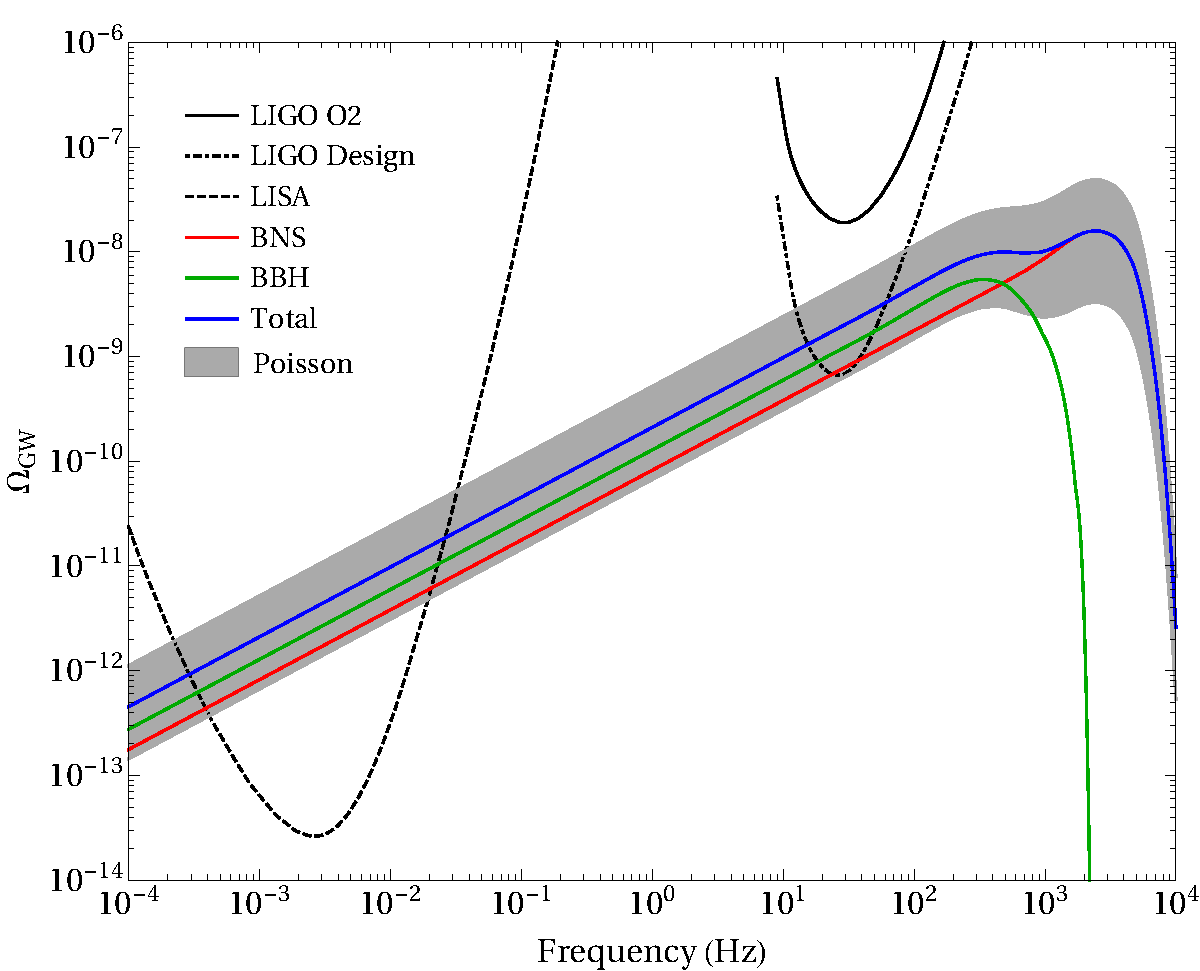
\includegraphics[width=\textwidth]{OmegaGW-sBH.pdf}
    \bicaption[来自天体物理双黑洞以及双中子星产生的随机引力波背景。绿线是双黑洞对应的随机引力波背景,而红线是双中子星对应的引力波背景。蓝色则表示总的随机引力波背景(包括双黑洞和双中子星的贡献);而灰色区域则表示总的引力波背景的泊松误差。在这里,我们取天体物理双黑洞的局域并合率为$R = 103_{-63}^{+110}$\,$\gpcyr$;而双中子星的局域并合率为$R = 1540_{-1220}^{+3200}$\,$\gpcyr$。图中的黑色实线表示LIGO第二个观测阶段的幂率积分曲线;点虚线表示LIGO设计阶段对应的幂率积分曲线;而虚线则表示LISA观测四年对应的幂率积分曲线。从图上可以看出,LIGO设计阶段和LISA对应的幂率积分曲线都能跨过泊松误差区域,表明天体物理双黑洞和双中子星产生的随机引力波背景可以被LIGO设计阶段和LISA探测到。]{\label{OmegaGW-sBH}
        来自天体物理双黑洞以及双中子星产生的随机引力波背景。绿线是双黑洞对应的随机引力波背景,而红线是双中子星对应的引力波背景。蓝色则表示总的随机引力波背景(包括双黑洞和双中子星的贡献);而灰色区域则表示总的引力波背景的泊松误差。在这里,我们取天体物理双黑洞的局域并合率为$R = 103_{-63}^{+110}$\,$\gpcyr$\citep{Abbott:2017vtc};而双中子星的局域并合率为$R = 1540_{-1220}^{+3200}$\,$\gpcyr$\citep{TheLIGOScientific:2017qsa}。图中的黑色实线表示LIGO第二个观测阶段的幂率积分曲线;点虚线表示LIGO设计阶段对应的幂率积分曲线;而虚线则表示LISA观测四年对应的幂率积分曲线。从图上可以看出,LIGO设计阶段和LISA对应的幂率积分曲线都能跨过泊松误差区域,表明天体物理双黑洞和双中子星产生的随机引力波背景可以被LIGO设计阶段和LISA探测到。
    }{The predicted stochastic gravitational-wave background from the binary neutron stars and stellar-origin binary black holes. 
    The red and green curves are backgrounds from the binary neutron stars (BNSs) and binary black holes (BBHs),
    respectively. 
    The total background is shown in the blue curve, while
    its Poisson error bars are in the grey shaded region.
    Here, we adopt the local merger rate $R = 103_{-63}^{+110}$\,$\gpcyr$ 
    for stellar-origin binary black holes \citep{Abbott:2017vtc},
    and $R = 1540_{-1220}^{+3200}$\,$\gpcyr$ for binary neutron stars
    \citep{TheLIGOScientific:2017qsa}.
    We also show the expected PI curves for LISA with $4$ years of 
    observation (dashed) and
    LIGO's observing runs of O2 (black) and design sensitivity (dot-dashed).
    The PI curves for LISA and LIGO's design sensitivity cross the Poisson
    error region, indicating the possibility to detect this background.}
\end{figure}

在估算并合率\Eq{sBHR}时,最复杂地方乃是计算天体物理黑洞和中子星的生成率。生成率可估算为\citep{Dvorkin:2016wac}
\e
    R_{\mathrm{birth}}(t,m_{\mathrm{rem}})=\int \psi [t-\tau(m_{*})] \phi(m_{*})
    \delta(m_{*}- g_{\mathrm{rem}}^{-1}(m_{\mathrm{rem}})) \text{d}m_{*},
\q
其中$m_{*}$为前身星的质量,$m_{\mathrm{rem}}$为最后天体的质量,而$\tau(m_{*})$前身星的寿命。$\tau(m_{*})$通常可以忽略\citep{Schaerer:2001jc}。上式中的$\phi(m_{*})$为初始质量函数(initial mass function,简称IMF)。对于中子星,初始质量函数为$1\,\Msun$到$2\,\Msun$之间的平坦分布;而对天体物理黑洞,初始质量函数$\phi(m_{*}) \propto m_{*}^{-2.35}$。此外,$\psi(t)$为恒星形成率(star formation rate,简称SFR),其为\citep{Nagamine:2003bd}
\e
\psi(z)= k \frac{a \exp[b(z-z_{m})]}{a-b+b \exp[a(z-z_{m})]}. 
\q
下面的计算中将使用文献\cite{Dvorkin:2016wac}给出的``\textit{Fiducial+PopIII}"模型的参数来计算上式。``\textit{Fiducial+PopIII}"是\textit{Fiducial}模型(其中$k=0.178 \Msun \mathrm{yr}^{-1} \mathrm{Mpc}^{-3}$,$z_{m}=2$, $a=2.37$,$b=1.8$)和\textit{PopIII}模型(其中$k=0.002 \Msun \mathrm{yr}^{-1} \mathrm{Mpc}^{-3}$,$z_{m}=11.87$,$a=13.8$,$b=13.36$)的综合。对于中子星,$g^{-1}_{\mathrm{ns}}(m_{\mathrm{ns}})=m_{\mathrm{ns}}$, 所以生成率的计算相对简单。而对于天体物理黑洞,其前身星的质量和最后残余质量存在特定的函数关系$m_{\mathrm{bh}}=g_{\mathrm{bh}}(m_{*})$。而这个函数关系是模型依赖的。在这里我们考虑``\textit{WWp}"模型\citep{Woosley:1995ip}。这个模型和广为使用的``\textit{Fryer}"模型\citep{Dvorkin:2016wac}在低红移时是不可区分的,但足够简单。对于初始质量为$m_{*}$的前身星,其残余的黑洞质量$m_{\mathrm{bh}}$为
\e
\frac{m_{\mathrm{bh}}}{m_{*}}=A \left(\frac{m_{*}}{40\Msun} \right)^{\beta} \frac{1}{\left( \frac{Z(z)}{0.01 Z_\odot} \right)^{\gamma} +1},
\q
其中$Z(z)$为金属丰度,其具体的函数形式由文献\cite{Belczynski:2016obo}给出。上式中各个参数的取值为$A=0.3$,$\beta =0.8$和$\gamma =0.2$ \citep{Dvorkin:2016wac}。通过解以上方程,就能得到$m_{*} = g_{\mathrm{bh}}^{-1}(m_{\mathrm{bh}})$。

\begin{table}[htb!]
    \centering
    \begin{tabular}{c|c|c}
        &\ $\Omega_{\mathrm{GW}}(25 \, \mathrm{Hz})$ \
        &\ $\Omega_{\mathrm{GW}}(3 \times 10^{-3} \, \mathrm{Hz})$\,\\
        \hline
        BNS\, &  $0.7^{+1.5}_{-0.6} \times 10^{-9}$ 
        & $1.7^{+3.5}_{-1.4} \times 10^{-12}$ \\
        [.3em]
        \hline
        BBH\, & $1.1^{+1.2}_{-0.7} \times 10^{-9}$  
        & $2.7^{+2.8}_{-1.6} \times 10^{-12}$ \\
        [.3em]
        \hline
        Total\, & $1.8^{+2.7}_{-1.3} \times 10^{-9}$  
        & $4.4^{+6.3}_{-3.0} \times 10^{-12}$ \\
        [.2em]
    \end{tabular}
    \bicaption{\label{Omegaf-sBH}
        天体物理双黑洞产生的随机引力波背景、双中子星产生的随机引力波背景以及总的随机引力波背景在LIGO和LISA最灵敏的频率附近(分别为$25 \, \mathrm{Hz}$和$3 \times 10^{-3} \, \mathrm{Hz}$)的大小。我们还给出了$90\%$的泊松误差范围。
    }{Estimates of the background energy density $\ogw (\nu)$ at the most
    sensitive frequencies of LIGO (near $25$ Hz) and LISA 
    (near $3\times 10^{-3}$ Hz) for each of the binary neutron star (BNS), stellar-origin binary black hole (BBH) and total background contributions, along with the $90\%$ Poisson error bounds.}
\end{table}


\begin{figure}[htb!]
    \centering
    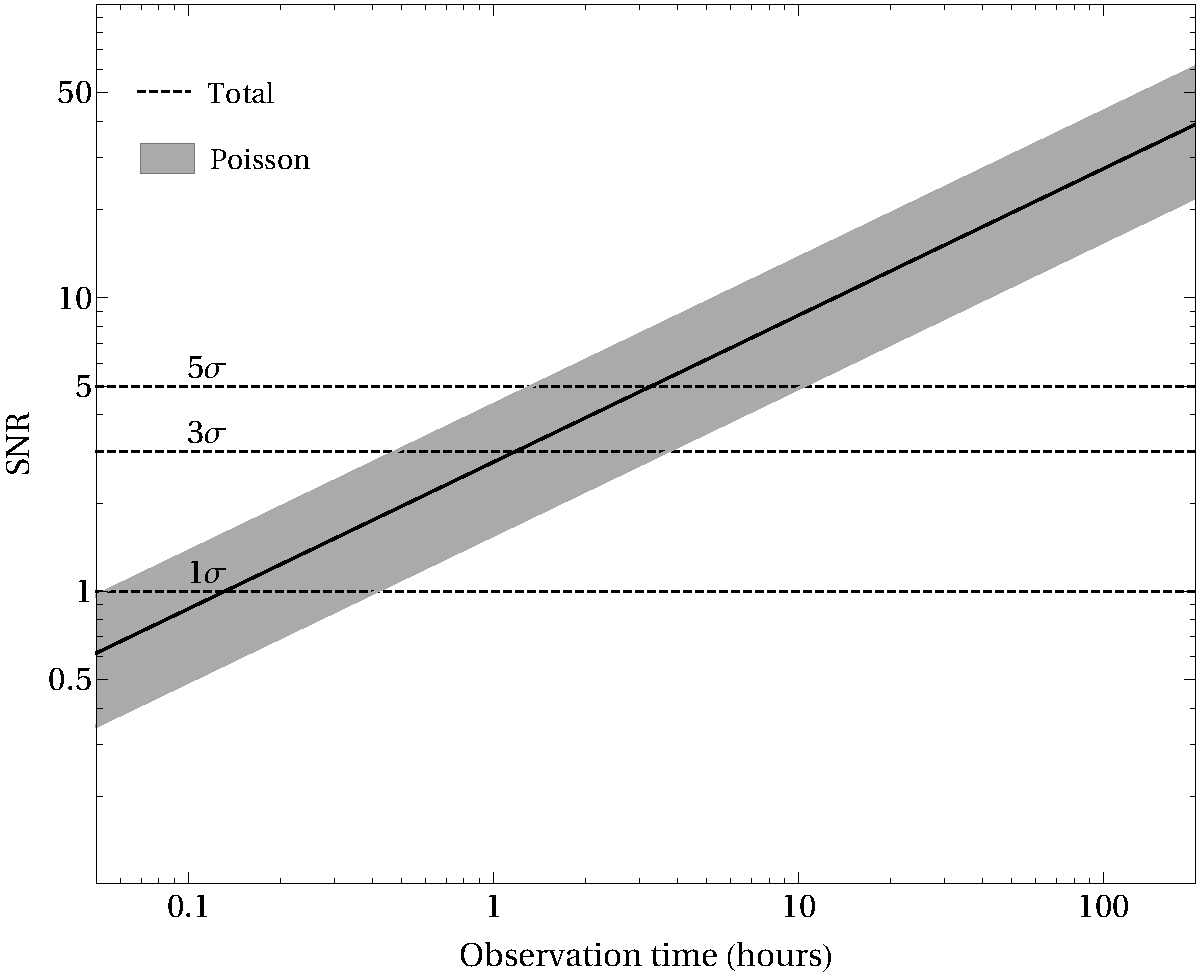
\includegraphics[width=\textwidth]{SNR-sBH.pdf}
    \bicaption[LISA探测器对探测天体物理双黑洞和双中子星产生的总的随机引力波背景的信噪比随观测时间的关系。黑色实线表示信噪比的中心值,而灰色区域表示信噪比的误差范围。在这里,我们取天体物理双黑洞的局域并合率为$R = 103_{-63}^{+110}$\,$\gpcyr$;而双中子星的局域并合率为$R = 1540_{-1220}^{+3200}$\,$\gpcyr$。在大约观测$20$个小时后,LISA可以探测到中心值大小的总的随机引力波背景;探测的信噪比为$\mathrm{SNR}=5$。]{\label{SNR-sBH} 
        LISA探测器对探测天体物理双黑洞和双中子星产生的总的随机引力波背景的信噪比随观测时间的关系。黑色实线表示信噪比的中心值,而灰色区域表示信噪比的误差范围。在这里,我们取天体物理双黑洞的局域并合率为$R = 103_{-63}^{+110}$\,$\gpcyr$\citep{Abbott:2017vtc};而双中子星的局域并合率为$R = 1540_{-1220}^{+3200}$\,$\gpcyr$\citep{TheLIGOScientific:2017qsa}。在大约观测$20$个小时后,LISA可以探测到中心值大小的总的随机引力波背景;探测的信噪比为$\mathrm{SNR}=5$。
    }{The SNR of LISA as a function of observing time for median total 
    stochastic gravitational-wave background (black curve) and associated uncertainties (grey shaded region),
    from the stellar-origin binary black holes and binary neutron stars.
    Here, we adopt the local merger rate $R = 103_{-63}^{+110}$\,$\gpcyr$ 
    for stellar-origin binary black holes \citep{Abbott:2017vtc},
    and $R = 1540_{-1220}^{+3200}$\,$\gpcyr$ for binary neutron stars
    \citep{TheLIGOScientific:2017qsa}.
    The predicted median total background can be detected with 
    $\mathrm{SNR}=5$ after about $20$ hours of observation time.}
\end{figure}

\begin{figure}[htb!]
    \centering
    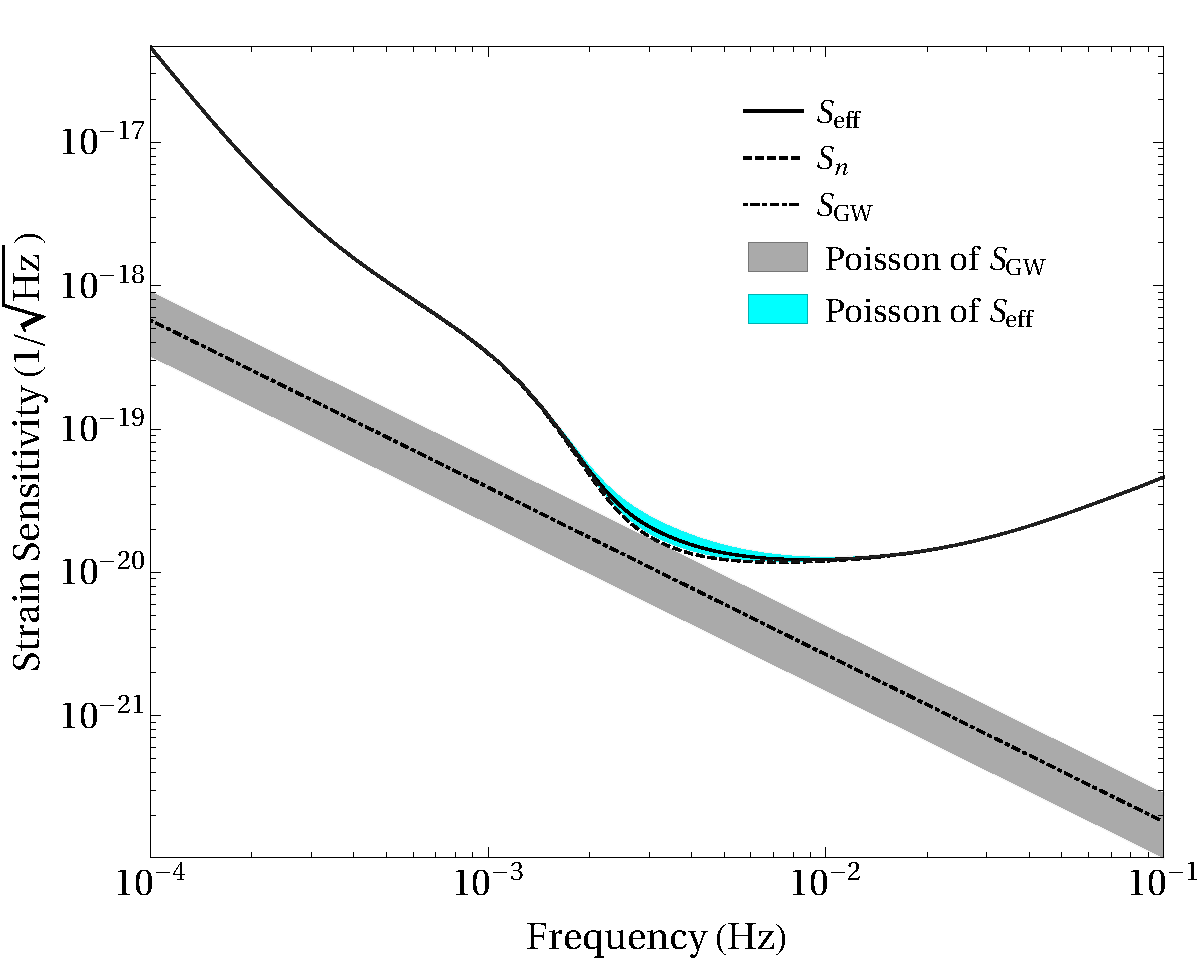
\includegraphics[width=\textwidth]{lisa-sensitivity-sBH.pdf}
    \bicaption{\label{lisa-sensitivity-sBH}
        由天体物理双黑洞和双中子星产生的总的随机引力波背景导致LISA探测器的有效应变灵敏度$S_{\mathrm{eff}}$(黑色实线)以及相应的泊松误差(青色区域)。图中还给出了LISA探测器的应变灵敏度$S_n$(虚线)以及随机引力波背景对应的应变灵敏度$S_{\mathrm{GW}}$(点虚线)和相应的泊松误差(灰色区域)。
    }{The effective strain sensitivity $S_{\mathrm{eff}}$ (black solid curve) of LISA and its Poisson uncertainties (cyan region), due to the effect of the total stochastic gravitational-wave background from stellar-origin binary black holes and binary neutron stars. We also show LISA's strain sensitivity $S_n$ (dashed curve), and $S_{\mathrm{GW}}$ (dot-dashed curve) along with its Poisson uncertainties (grey shaded region).}
\end{figure} 

\begin{figure}[htbp!]
    \centering
    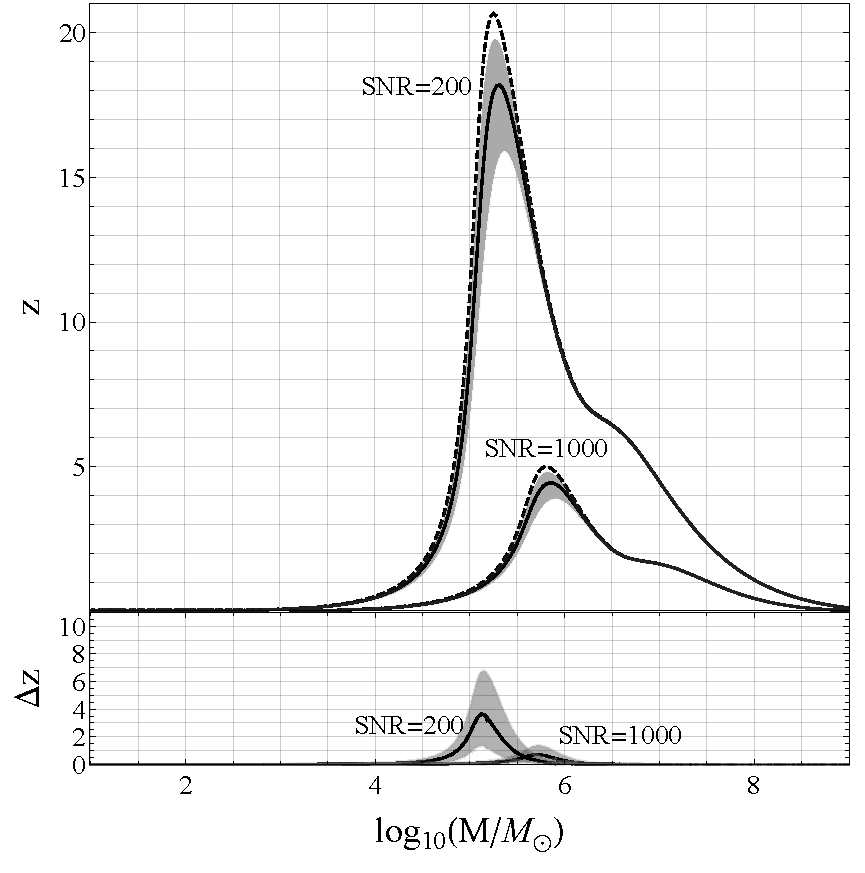
\includegraphics[width=\textwidth]{z-sBH.pdf}
    \bicaption[由天体物理双黑洞和双中子星产生的总的随机引力波背景对LISA探测器对于大质量双黑洞系统最大可探测红移$z$的影响。我们用$M$表示大质量双黑洞的总质量。我们固定质量比为$q=0.2$。我们分别考虑$\SNR=200$和$\SNR=1000$的两种情况。上图的虚线表示LISA最大可探测红移的等高线,而黑色实线表示考虑了随机引力波背景后LISA的最大可探测红移的等高线。灰色区域是黑色实线对应的泊松误差范围。下图给出了考虑随机引力波背景后对LISA最大可探测红移所引起的变化及误差范围。]{\label{z-sBH}
        由天体物理双黑洞和双中子星产生的总的随机引力波背景对LISA探测器对于大质量双黑洞系统最大可探测红移$z$的影响。我们用$M$表示大质量双黑洞的总质量。仿照\cite{Audley:2017drz},我们固定质量比为$q=0.2$。我们分别考虑$\SNR=200$和$\SNR=1000$的两种情况。上图的虚线表示LISA最大可探测红移的等高线,而黑色实线表示考虑了随机引力波背景后LISA的最大可探测红移的等高线。灰色区域是黑色实线对应的泊松误差范围。下图给出了考虑随机引力波背景后对LISA最大可探测红移所引起的变化及误差范围。
    }{The impacts of the total stochastic gravitational-wave background from stellar-origin binary black holes and binary neutron stars 
        on the largest detectable redshift $z$ of MBHB (with total mass $M$) coalescences for LISA.
        The mass ratio is set to $q=0.2$ following \cite{Audley:2017drz}. 
        The upper panel shows the contours of $\SNR=200$ and $\SNR=1000$ 
        for LISA (dashed curves), 
        together with the effect of stochastic gravitational-wave background (black curves) and the Poisson error 
        bars (grey shaded region). 
        The lower panel shows the residuals of corresponding contours. }
\end{figure}

对并合率密度中的质量做积分,即可得到并合率随红移的演化函数
\e
\mR(z)  =\int \mR(z,m_{1},m_{2} )\, \rmd m_{1} \text{d}m_{2}.
\q
对于天体物理双黑洞,引力波对其局域并合率$R \equiv \mR(z=0)$的限制为$R = 103_{-63}^{+110}$\,$\gpcyr$\citep{Abbott:2017vtc};而对于双子星,引力波的限制为$R = 1540_{-1220}^{+3200}$\,$\gpcyr$\citep{TheLIGOScientific:2017qsa}。利用公式\Eq{OmegaGW},我们就可以计算来自天体物理双黑洞以及双中子星产生的随机引力波背景。在\Fig{OmegaGW-sBH}中,我们给出了相应的随机引力波背景的能量密度谱。为了和引力波实验观测数据比较,我们还画出了LIGO探测器\citep{TheLIGOScientific:2017qsa}的幂率积分(power-law integrated,简称PI)曲线和LISA探测器\citep{Cornish:2017vip,Cornish:2018dyw}的幂率积分曲线。结果表明,不管是天体物理双黑洞产生的引力波背景还是双中子星产生的引力波背景,在未来都很可能被LIGO和LISA探测到。另外,在LIGO和LISA的可探测频段内,天体物理双黑洞和双中子星产生的引力波背景都近似和频率的$2/3$次方成正比,即$\ogw \propto \nu^{2/3}$。这是因为在可探测的频段内,随机引力波背景的贡献主要来自于双黑洞或双中子星的旋进阶段,而在旋进阶段,单个双黑洞或双中子星辐射的引力波能量谱大概就和频率的$2/3$次方成正比。在\Table{Omegaf-sBH}中,我们总结了在LIGO和LISA最灵敏的频率附近的随机引力波背景的能量密度的大小$\ogw (\nu)$。对于LIGO探测器来说,其最灵敏的频率大概是$25$Hz左右,而LISA探测器最灵敏的频率大概是$3\times 10^{-3}$Hz左右。


对于LISA探测器,假如其观测时间为$T$,其所能观测到随机引力波背景的信噪比(signal-to-noise ratio,简称SNR)为\citep{Thrane:2013oya,Caprini:2015zlo}
\e
\text{SNR}=\sqrt{T} \left[ \int \rmd \nu \frac{\Omega_{\mathrm{GW}}(\nu)}{\Omega_{n}(\nu)} \right] ^{1/2},
\q
其中$\Omega_{n}(\nu)$定义为
\e 
\Omega_{n}(\nu)\equiv 2 \pi^2 \nu^3 S_{n}(\nu)/\left(3 H_{0}^2 \right),
\q 
而$S_{n}$为LISA的噪音应变灵敏度。\Fig{SNR-sBH}给出了预期累积信噪比关于时间的函数关系。由图可知,在观测$20$小时后,LISA可以探测到来自天体物理双黑洞和双中子星的中心值大小的随机引力波背景,相应的信噪比为$\mathrm{SNR} = 5$。在最乐观的情况下LISA观测$5$个小时就能探测到信噪比$\mathrm{SNR} = 5$的总的随机引力波背景,而在最悲观的情况下LISA观测$8$天能探测到信噪比$\mathrm{SNR} = 5$的总的随机引力波背景。

由以上分析可知,如果不在LISA的噪音背景中把来自天体物理双黑洞和双中子星产生的总的随机引力波背景扣除掉,这些引力波背景可能成为LISA新的噪音源,从而影响LISA的科学探测目标。例如,对于LISA来说,探测大质量双黑洞(massive black hole binary,简称MBHB)的并合是LISA的一个关键科学目标\citep{Audley:2017drz},而如果不把这些引力波背景从噪音中扣除掉的话,会降低LISA对于大质量双黑洞的最大可探测红移。 


仿照\cite{Barack:2004wc,Cornish:2018dyw},我们定义随机引力波背景产生的等效噪音应变灵敏度为
\e
S_{\mathrm{GW}}(\nu) \equiv \frac{3 H_{0}^2}{2 \pi^2}
\frac{\Omega_{\mathrm{GW}}(\nu)}{\nu^3}.
\q
将随机引力波背景产生的等效噪音应变灵敏度加到LISA的噪音应变灵敏度$S_{n}(\nu)$中,即可得到有效的总的应变灵敏度$S_{\mathrm{eff}}(\nu)$,即
\e 
S_{\mathrm{eff}}(\nu)=S_{n}(\nu)+S_{\mathrm{GW}}(\nu).
\q
在\Fig{lisa-sensitivity-sBH}中,我们给出了相应的应变灵敏度曲线。对于探测单个源传播过来的引力波应变信号(也就是通常说的波形)$h(t)$,LISA对应的信噪比为
\e
\SNR = 2 \left[ \int \rmd \nu 
\frac{|\tilde{h}(\nu)|^2}{S_{\mathrm{eff}}(\nu)} \right]^{1/2},
\q
其中$\tilde{h}(\nu)$是$h(t)$在频率空间的波形。在这里我们使用\cite{Ajith:2007kx}给出的唯象波形来描述大质量双黑洞系统产生的引力波。

对于LISA来说,研究大质量黑洞的增长机制是其重要的科学探索目标之一\citep{Audley:2017drz}。为了实现这一目标,要求LISA对大质量黑洞无量纲自旋的探测的绝对误差要小于$0.1$,并且探测到的自旋方向的误差要小于$10^{\circ}$。为了达到这些要求,需要探测的信噪比达到$200$以上。在这里我们考虑了$\SNR=200$和$\SNR=1000$的两种情况。\Fig{z-sBH}给出了随机引力波背景对LISA探测大质量双黑洞并合的信噪比的影响,表明最大可探测红移会由于未解析出来的随机引力波背景的影响而减小。这也表明LISA可探测的区域被压低了,从而减少LISA可探测到的大质量双黑洞并合的事件数。目前的研究表明,为了形成大质量黑洞通常需要种子黑洞的质量在$10^3 \Msun$到$10^5 \Msun$的量级,而且相应的红移在在$10\lesssim z \lesssim 15$\citep{Volonteri:2010wz}。从\Fig{z-sBH}看出,由于随机引力波背景导致的等效噪音可以压低LISA对$10^5 \Msun$以上的种子黑洞并合的最大可探测红移。因此,为了提高LISA探测器的探测灵敏度,需要设法将这些随机引力波背景从背景噪音中扣除掉。

%%%%%%%%%%%%%%%%%%%%%%%%%%%%%%%%%%%%%%%%%%%%%%%%%%%%%%%%%%%%%%%%%%%%%%
\section{\label{PBH}原初双黑洞产生的随机引力波背景}
在本节中,我们将计算原初双黑洞产生的随机引力波背景。我们假设\lvc 目前所探测到的所有双黑洞都来自原初黑洞。
在这里,我们使用文献\cite{Chen:2018czv}给出的原初双黑洞的并合率,也就是我们在上一章所推导出来的并合率表达式。在计算并合率时,我们考虑了所有原初黑洞和线性密度扰动对原初双黑洞角动量的贡献。对于一个一般的已经归一化的原初黑洞质量概率分布函数$P(m|\vth)$,其共动并合率密度分布为\citep{Chen:2018czv}
\m\label{calR2} 
\mR_{12}(t|\vth) & \app & 3.9\cdot 10^6\times \({t\over t_0}\)^{-{34\over 37}} f^2 (f^2+\sigma_{\mathrm{eq}}^2)^{-{21\over 74}} (m_1 m_2)^{{3\over 37}} (m_1+m_2)^{36\over 37} \nonumber \\
&& \times  \min\(\frac{P(m_1|\vth)}{m_1}, \frac{P(m_2|\vth)}{m_2}\) \({P(m_1|\vth)\over m_1}+{P(m_2|\vth)\over m_2}\),
\n
其中$\vth$是质量函数中所带有的参数,$t_0$为宇宙年龄。需要注意的是,上式的并合率密度的单位为$\gpcyr$。此外,$\sigma_{\mathrm{eq}}$是其余暗物质在辐射-物质平衡时期在${\cal O}(10^0\sim10^3) M_\odot$尺度上的密度扰动的方差。类似于\cite{Ali-Haimoud:2017rtz,Chen:2018czv},我们取$\sigma_{\mathrm{eq}}\approx 0.005$。而且原初黑洞的质量$m_1$和$m_2$都是以$\Msun$为单位的。在这里$f$是总原初黑洞占非相对论物质的丰度,其和原初黑洞占冷暗物质的丰度$\fpbh$的关系为$\fpbh\equiv \Omega_{\mathrm{PBH}}/\Omega_{\mathrm{CDM}} \approx f/0.85$。

对并合率密度分布\eqref{calR2}的质量做积分,即可得到并合率随时间或红移的演化
\e
\mR(t|\vth) = \int \mR_{12}(t|\vth)\ \rmd m_1\, \rmd m_2.
\q 
由此可以得到局域的并合率密度分布
\e 
\mR_{12}(t_0|\vth) = R\, p(m_1,m_2|\vth),
\q 
其中$p(m_1,m_2|\vth)$为并合双黑洞中黑洞质量的概率分布,而局域并合率$R \equiv \mR(t_0|\vth)$是一个归一化系数。由定义可知,$p(m_1,m_2|\vth)$满足归一化条件,即
\e 
 \int p(m_1,m_2|\vth) \rmd m_1\, \rmd m_2 = 1.
\q 
需要注意的是,这里的质量是源参考系的质量,而不是探测器参考系的质量。

下面我们需要将理论得到的原初双黑洞的并合率和引力波实验数据做拟合,从而推断出模型参数$\{\vth, R\}$的取值。在这里我们不需用用到\lvc 最原始的应变数据,而只需要用到\lvc 公布的双黑洞并合事件的后验分布数据,然后用到层次贝叶斯推断(hierarchical Bayesian inference)的方法去做模型的参数估计。层次贝叶斯推断方法的优点是可以节省大量的计算量。这一方法已经被广泛应用于引力波领域\citep{Abbott:2016nhf,Abbott:2016drs,TheLIGOScientific:2016pea,Wysocki:2018mpo,Fishbach:2018edt,Mandel:2018mve,Thrane:2018qnx}。下面简单介绍这一方法。假定已有$N$个双黑洞并合事件的数据$\vd = (d_1, \dots, 
d_N)$,那么由理论模型得到数据的似然函数(likelihood function)为\citep{Wysocki:2018mpo,Fishbach:2018edt,Mandel:2018mve,Thrane:2018qnx}
\e\label{likelihood1}
p(\vd|\vth, R) \propto R^{N} e^{-R\, \beta(\vth)} \prod_i^N 
\int \rmd\vla\ p(d_i|\vla)\ p(\vla|\vth),
\q 
其中$\vla \equiv \{m_1, m_2\}$。在上式中$p(d_i|\vla)$为单个引力波事件在给定双黑洞参数$\vla$时得到数据$d_i$的似然函数。由于\lvc 在分析单个引力波事件时,其用到的黑洞的质量参数的先验分布(prior distribution)为平的分布,所以对于单个事件而言,其似然函数$p(d_i|\vla)$和后验分布成正比$p(\vla|d_i)$,即$p(d_i|\vla) \propto p(\vla|d_i)$。因此我们可以直接用\lvc 公开的每个双黑洞并合事件的后验分布\citep{Vallisneri:2014vxa,TheLIGOScientific:2016pea,Biwer:2018osg}来计算\Eq{likelihood1}的积分。同时,\Eq{likelihood1}的$\beta(\vth)$定义为
\e 
\beta(\vth) \equiv \int \rmd\vla\ VT(\vla)\ p(\vla|\vth),
\q 
其中$VT(\vla)$为\lvc 可探测的时空体积。我们用半解析的方法\cite{Abbott:2016nhf,Abbott:2016drs}来计算$VT$。在这里我们忽略了黑洞的自旋效应,并且使用``早期高灵敏度”(``Early High Sensitivity")的噪音功率谱(power spectral density, 简称PSD)来近似LIGO的前两个观测阶段的噪音功率谱。我们取单个引力波探测器的信噪比为$\SNR = 8$作为探测到引力波事件的阀值。真实的LIGO探测器是由两个探测器组成的引力波探测器网络。对于整个探测器网络来说,相应的信噪比阀值大约是$12$。

给定先验分布$p(\vth, R)$后,我们就能得到对应的后验分布
\e\label{post1} 
p(\vth, R|\vd) \propto p(\vd |\vth, R)\ p(\vth, R).
\q 
对于$\vth$参数我们选平的分布,而对于局域并合率$R$我们选对数平的分布。换言之,我们假定的先验分布为
\e 
p(\vth, R) \propto \frac{1}{R}.
\q 
有了先验分布,再利用似然函数\eqref{likelihood1}式,我们可以得到对局域并合率$R$做边际化后的后验分布,即
\e\label{post_vth1} 
p(\vth|\vd) \propto \[\beta(\vth)\]^{-N} 
\prod_i^N \int \rmd\vla\ p(d_i|\vla)\ p(\vla|\vth).
\q
这个后验分布公式已经被广泛应用于引力波的参数推断中\citep{Abbott:2016nhf,Abbott:2017vtc,TheLIGOScientific:2016pea,Abbott:2016drs,Fishbach:2017zga}。我们将仿照文献\cite{Abbott:2016nhf,TheLIGOScientific:2016pea,Abbott:2016drs,Abbott:2017vtc}的做法,先用\Eq{post_vth1}来限制$\vth$参数,然后在\Eq{post1}中将$\vth$固定成最佳拟合值来估计局域并合率$R$的值。和\ref{SBH}小节一样,我们考虑的双黑洞的质量范围为$5\Msun \leq m_2 \leq m_1$且$m_1 + m_2 \leq 100\Msun$。这里我们只用LIGO第一个观测阶段观测到的$3$个双黑洞并合事例来拟合模型参数。LIGO的第一个观测阶段观测的有效时间为$48.6$天\citep{TheLIGOScientific:2016pea}。在\Table{events2}中,我们列出了这$3$个双黑洞并合事件的源的主要性质。

%%%%%%%%%%%%%%%%%%%%%%%%%%%%%%%%%%%%%%%%%%%%%%%%%%%%%%%%%%%%%%%%%%%%%%
\begin{table}[htb!]
    \centering
    \begin{tabular}{c|c|c|c}
        事件 & 较重黑洞的质量 & 较轻黑洞的质量 & 红移\\
        \hline
        GW150914\, 
        &  $36.2\,^{+5.2}_{-3.8}$\,$\Msun$ & $29.1\,^{+3.7}_{-4.4}$\,$\Msun$ 
        & $0.09\,^{+0.03}_{-0.04}$\\
        [.3em]
        \hline
        LVT151012\, 
        & $23\,^{+18}_{-6}$\,$\Msun$  & $13\,^{+4}_{-5}$\,$\Msun$ 
        & $0.20\,^{+0.09}_{-0.09}$\\
        [.3em]
        \hline
        GW151226\, 
        &  $14.2\,^{+8.3}_{-3.7}$\,$\Msun$  & $7.5\,^{+2.3}_{-2.3}$\,$\Msun$ 
        & $0.09\,^{+0.03}_{-0.04}$\\
        [.3em]
        \hline
    \end{tabular}
    \bicaption[\lvc 第一个观测阶段探测到的$3$个双黑洞并合事件的源的主要性质。]{\lvc 第一个观测阶段探测到的$3$个双黑洞并合事件的源的主要性质\citep{Abbott:2016blz,TheLIGOScientific:2016pea,TheLIGOScientific:2016qqj,TheLIGOScientific:2016pea,Abbott:2016nmj}。
    }{A summary of the masses and source redshifts of the $3$ 
    binary black holes detected by \lvc\, collaborations
    ~\citep{Abbott:2016blz,TheLIGOScientific:2016pea,TheLIGOScientific:2016qqj,TheLIGOScientific:2016pea,Abbott:2016nmj}.}
    \label{events2}
\end{table}
%%%%%%%%%%%%%%%%%%%%%%%%%%%%%%%%%%%%%%%%%%%%%%%%%%%%%%%%%%%%%%%%%%%%%%

在以下的两个小节中我们将考虑两种不同的原初黑洞的质量分布函数。我们先用LIGO的引力波数据来限制模型参数$\{\vth, R\}$,然后由此计算相应的随机引力波背景。

%%%%%%%%%%%%%%%%%%%%%%%%%%%%%%%%%%%%%%%%%%%%%%%%%%%%%%%%%%%%%%%%%%%%%%
\subsection{幂率质量函数}
这里我们考虑幂率形式的原初黑洞质量分布函数\citep{Carr:1975qj}
\e\label{power}
P(m)\approx {\alpha-1\over \Mmin} \({m\over \Mmin}\)^{-\alpha},
\q
其中$m\geq \Mmin = 5\Msun$,且要求幂指数$\alpha>1$。在这种情况下,模型有两个自由参数,为$\{\vth, R\} = \{\al, R\}$。

\begin{figure}[htb!]
    \centering
    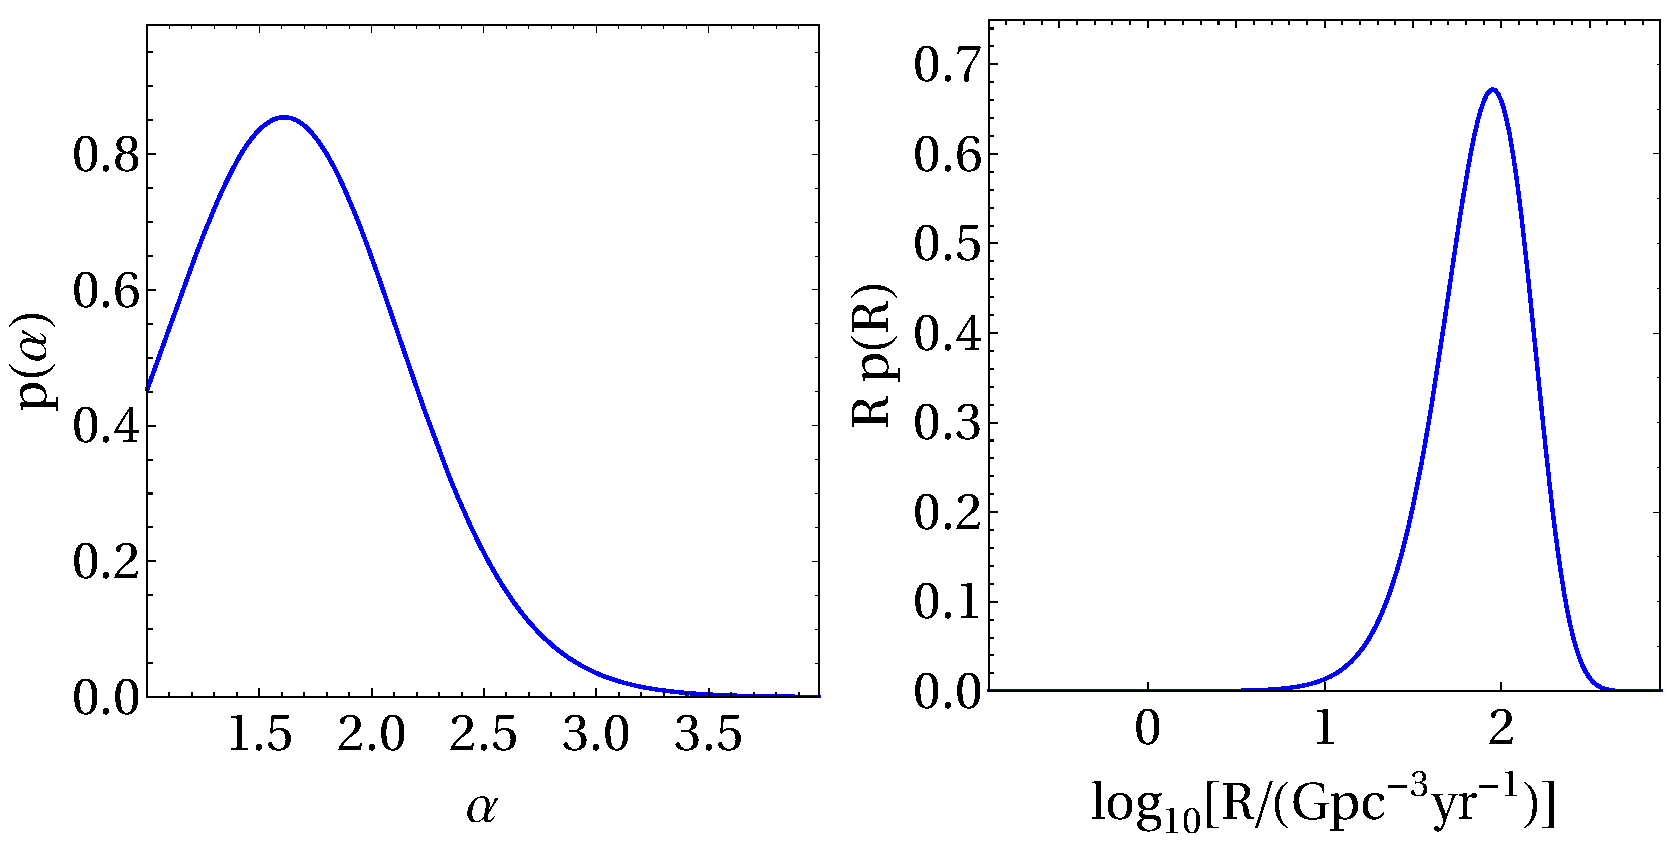
\includegraphics[width=\textwidth]{posterior-PBH-power.pdf}
    \bicaption{\label{posterior-PBH-power} 
        当原初黑洞质量函数为\textit{幂率}形式的情况下,用LIGO第一个观测阶段的$3$个双黑洞并合事件拟合得到模型参数$\{\vth, R\} = \{\al, R\}$的后验分布。
    }{The posterior distributions for $\{\vth, R\} = \{\al, R\}$ for
    \textit{power-law} mass function of PBHs, by using $3$ events from 
    LIGO's O1 observing run.}
\end{figure}

\begin{figure}[htbp!]
    \centering
    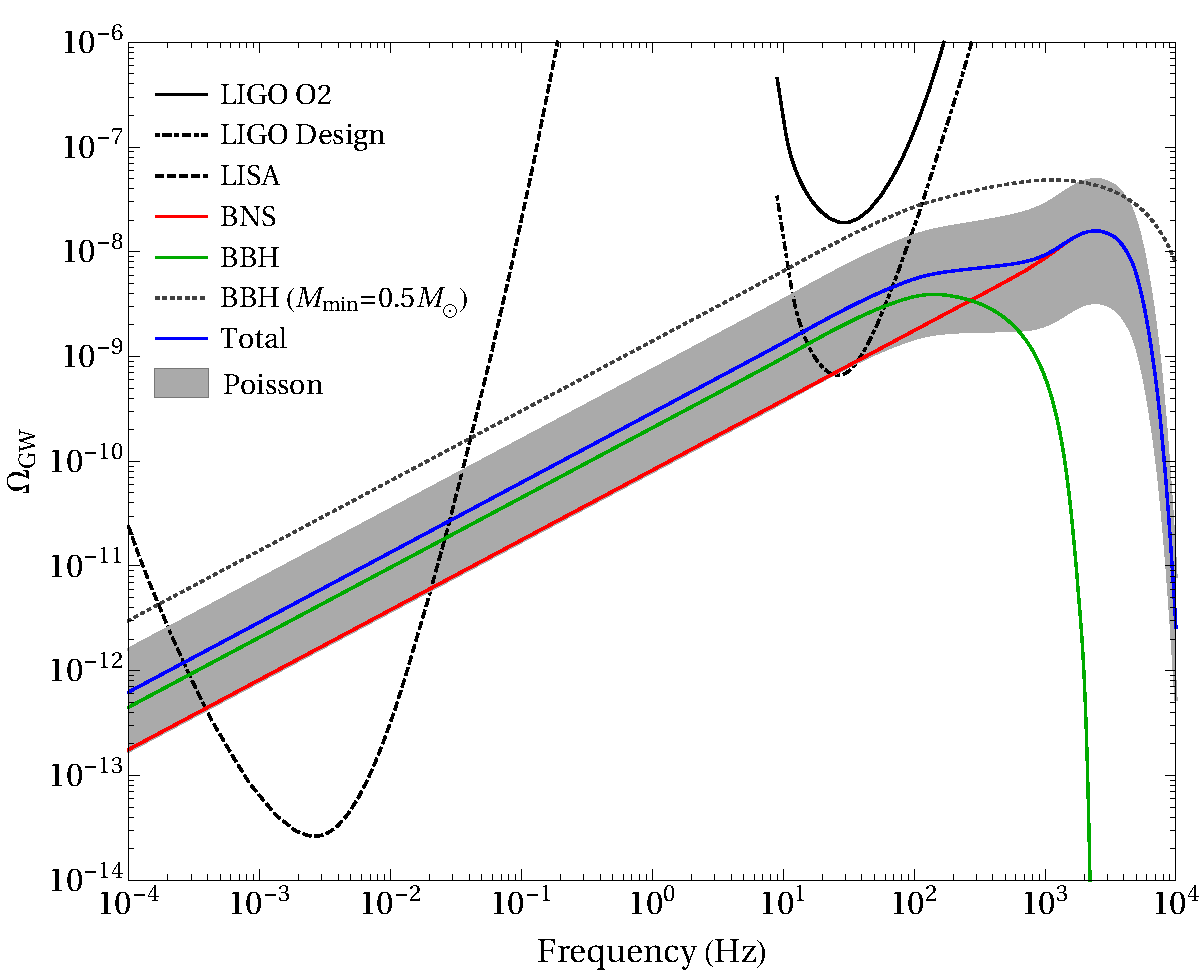
\includegraphics[width=0.8\textwidth]{OmegaGW-PBH-power.pdf}
    \bicaption[来自幂率质量分布的原初双黑洞以及双中子星产生的随机引力波背景。绿线是双黑洞对应的随机引力波背景,而红线是双中子星对应的随机引力波背景。蓝色表示总的随机引力波背;而灰色区域表示总的随机引力波背景的泊松误差。对于双黑洞,我们固定$\al$和局域并合率$R$为其最佳拟合值,即$\al = 1.61$和$R = 80\,^{+108}_{-56}$\, $\gpcyr$,且$\fpbh = 3.8\,^{+2.3}_{-1.8} \times 10^{-3}$。而对于双中子星,我们取局域并合率为$R = 1540_{-1220}^{+3200}$\,$\gpcyr$。图中的黑色实线表示LIGO第二个观测阶段(O2)的幂率积分曲线;点虚线表示LIGO设计阶段对应的幂率积分曲线;而虚线则表示LISA观测四年对应的幂率积分曲线。从图上可以看出,LIGO设计阶段和LISA对应的幂率积分曲线都能跨过泊松误差区域,表明原初双黑洞和双中子星产生的随机引力波背景可以被LIGO设计阶段和LISA探测到。]{\label{OmegaGW-PBH-power} 
        来自幂率质量分布的原初双黑洞以及双中子星产生的随机引力波背景。绿线是双黑洞对应的随机引力波背景,而红线是双中子星对应的随机引力波背景。蓝色表示总的随机引力波背;而灰色区域表示总的随机引力波背景的泊松误差。对于双黑洞,我们固定$\al$和局域并合率$R$为其最佳拟合值,即$\al = 1.61$和$R = 80\,^{+108}_{-56}$\, $\gpcyr$。该情况下对应的原初黑洞占暗物质的丰度为$\fpbh = 3.8\,^{+2.3}_{-1.8} \times 10^{-3}$。而对于双中子星,我们取局域并合率为$R = 1540_{-1220}^{+3200}$\,$\gpcyr$\citep{TheLIGOScientific:2017qsa}。图中的黑色实线表示LIGO第二个观测阶段(O2)的幂率积分曲线;点虚线表示LIGO设计阶段对应的幂率积分曲线;而虚线则表示LISA观测四年对应的幂率积分曲线。从图上可以看出,LIGO设计阶段和LISA对应的幂率积分曲线都能跨过泊松误差区域,表明原初双黑洞和双中子星产生的随机引力波背景可以被LIGO设计阶段和LISA探测到。
    }{The predicted stochastic gravitational-wave background from the binary neutron stars (BNSs)) and primordial-origin binary black holes (BBHs)
    with a \textit{power-law} mass function. 
    The red and green curves are backgrounds from the binary neutron stars and binary black holes, respectively. 
    The total background is shown in the blue curve, while
    its Poisson error bars are in the grey shaded region.
    For binary black holes, we adopt the best-fit value for $\al = 1.61$, 
    and the inferred local merger rate $R = 80\,^{+108}_{-56}$\, $\gpcyr$,
    which corresponds to $\fpbh = 3.8\,^{+2.3}_{-1.8} \times 10^{-3}$. 
    And for binary neutron stars, we adopt $R = 1540_{-1220}^{+3200}$\,$\gpcyr$ 
    \citep{TheLIGOScientific:2017qsa}.
    The dotted line shows the background from binary black holes with $\Mmin = 0.5 \Msun$, 
    by fixing $\al = 1.61$ and $R = 80$\, $\gpcyr$.
    We also show the expected PI curves for LISA with $4$ years of 
    observation (dashed) and
    LIGO's observing runs of O2 (black) and design sensitivity (dot-dashed).
    The PI curves for LISA and LIGO's design sensitivity cross the Poisson
    error region, indicating the possibility to detect this background.}
\end{figure}

\begin{table}[htb!]
    \centering
    \begin{tabular}{c|c|c}
        &\ $\Omega_{\mathrm{GW}}(25 \, \mathrm{Hz})$ \
        &\ $\Omega_{\mathrm{GW}}(3 \times 10^{-3} \, \mathrm{Hz})$\,\\
        \hline
        BNS\, &  $0.7^{+1.5}_{-0.6} \times 10^{-9}$ 
        & $1.7^{+3.5}_{-1.4} \times 10^{-12}$ \\
        [.3em]
        \hline
        BBH\, & $1.8_{-1.3}^{+2.5} \times 10^{-9}$  
        & $4.3^{+5.9}_{-3.0} \times 10^{-12}$ \\
        [.3em]
        \hline
        Total\, & $2.5^{+4.0}_{-1.9} \times 10^{-9}$  
        & $6.0^{+9.4}_{-4.4} \times 10^{-12}$ \\
        [.2em]
    \end{tabular}
    \bicaption{\label{Omegaf-PBH-power}
        原初双黑洞产生的随机引力波背景、双中子星产生的随机引力波背景以及总的随机引力波背景在LIGO和LISA最灵敏的频率附近(分别为$25 \, \mathrm{Hz}$和$3 \times 10^{-3} \, \mathrm{Hz}$)的大小。原初黑洞的质量函数为幂率形式。我们还给出了$90\%$的泊松误差范围。
    }{Estimates of the background energy density $\ogw (\nu)$ at the most sensitive frequencies of LIGO (near $25$ Hz) and LISA (near $3\times 10^{-3}$ Hz) for each of the binary neutron star (BNS), primordial-origin binary black hole (BBH, with a \textit{power-law} mass function) and total background contributions, along with the $90\%$ Poisson error bounds.}
\end{table}

\begin{figure}[htbp!]
    \centering
    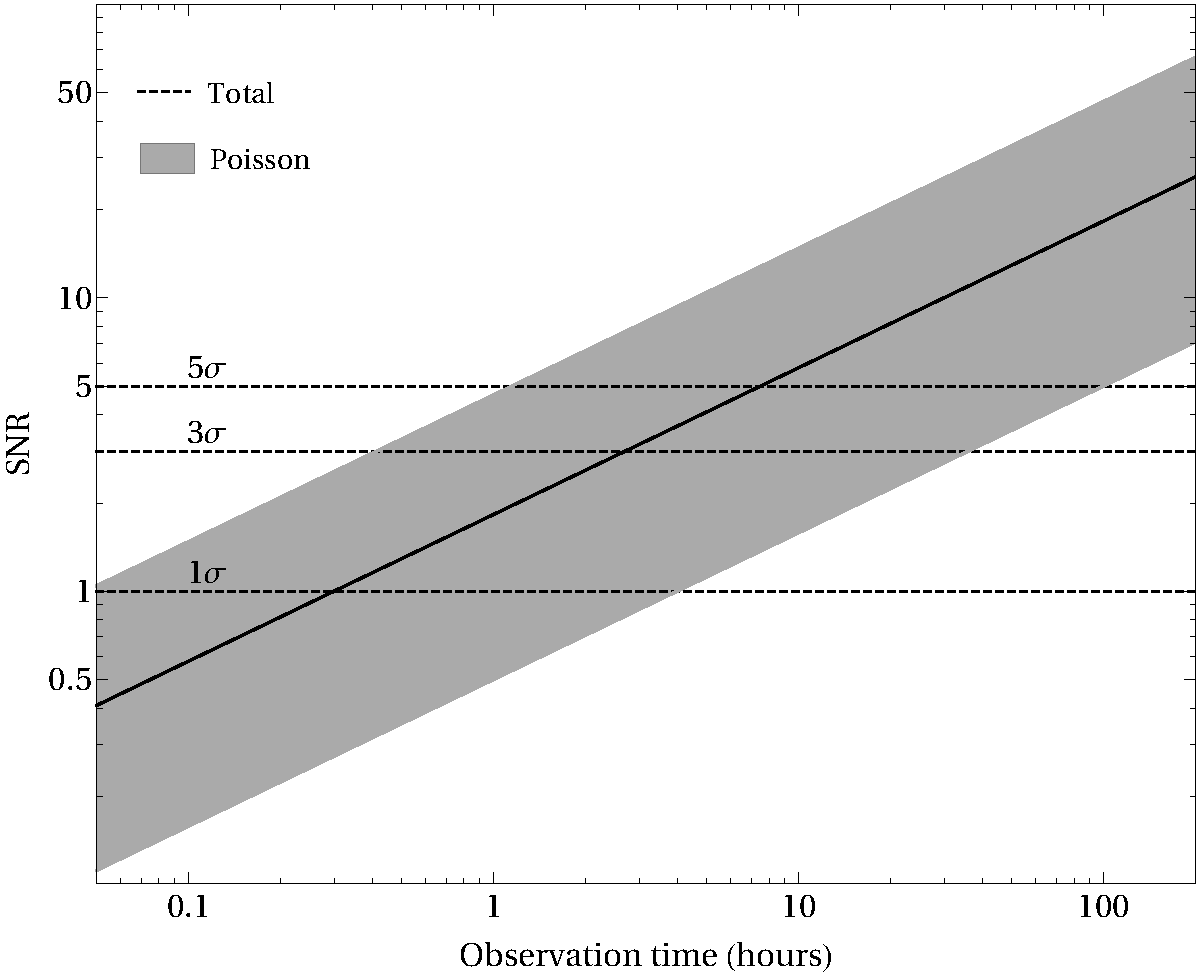
\includegraphics[width=\textwidth]{SNR-PBH-power.pdf}
    \bicaption[LISA探测器对探测原初双黑洞和双中子星产生的总的随机引力波背景的信噪比随观测时间的关系。原初黑洞的质量函数为幂率形式。黑色实线表示信噪比的中心值,而灰色区域表示信噪比的误差范围。对于双黑洞,我们固定$\al$和局域并合率$R$为其最佳拟合值,即$\al = 1.61$和$R = 80\,^{+108}_{-56}$\, $\gpcyr$。该情况下对应的原初黑洞占冷暗物质的丰度为$\fpbh = 3.8\,^{+2.3}_{-1.8} \times 10^{-3}$;而对于双中子星,我们取局域并合率为$R = 1540_{-1220}^{+3200}$\,$\gpcyr$。在大约观测$10$个小时后,LISA可以探测到中心值大小的总的随机引力波背景;探测的信噪比为$\mathrm{SNR}=5$。]{\label{SNR-PBH-power}
        LISA探测器对探测原初双黑洞和双中子星产生的总的随机引力波背景的信噪比随观测时间的关系。原初黑洞的质量函数为幂率形式。黑色实线表示信噪比的中心值,而灰色区域表示信噪比的误差范围。对于双黑洞,我们固定$\al$和局域并合率$R$为其最佳拟合值,即$\al = 1.61$和$R = 80\,^{+108}_{-56}$\, $\gpcyr$。该情况下对应的原初黑洞占冷暗物质的丰度为$\fpbh = 3.8\,^{+2.3}_{-1.8} \times 10^{-3}$;而对于双中子星,我们取局域并合率为$R = 1540_{-1220}^{+3200}$\,$\gpcyr$\citep{TheLIGOScientific:2017qsa}。在大约观测$10$个小时后,LISA可以探测到中心值大小的总的随机引力波背景;探测的信噪比为$\mathrm{SNR}=5$。
    }{The SNR of LISA as a function of observation time for median total 
        stochastic gravitational-wave background (black curve) and associated uncertainties (grey shaded region),
        from the primordial-origin binary black holes (with a \textit{power-law} mass function) and binary neutron stars.
        For binary black holes, we adopt the best-fit value for $\al = 1.61$, 
        and the inferred local merger rate $R = 80\,^{+108}_{-56}$\, $\gpcyr$,
        which corresponds to $\fpbh = 3.8\,^{+2.3}_{-1.8} \times 10^{-3}$. 
        And for binary neutron stars, we adopt $R = 1540_{-1220}^{+3200}$\,$\gpcyr$ 
        \citep{TheLIGOScientific:2017qsa}.
        The predicted median total background can be detected with 
        $\mathrm{SNR}=5$ after about $10$ hours of observation time.}
\end{figure}

\begin{figure}[htbp!]
    \centering
    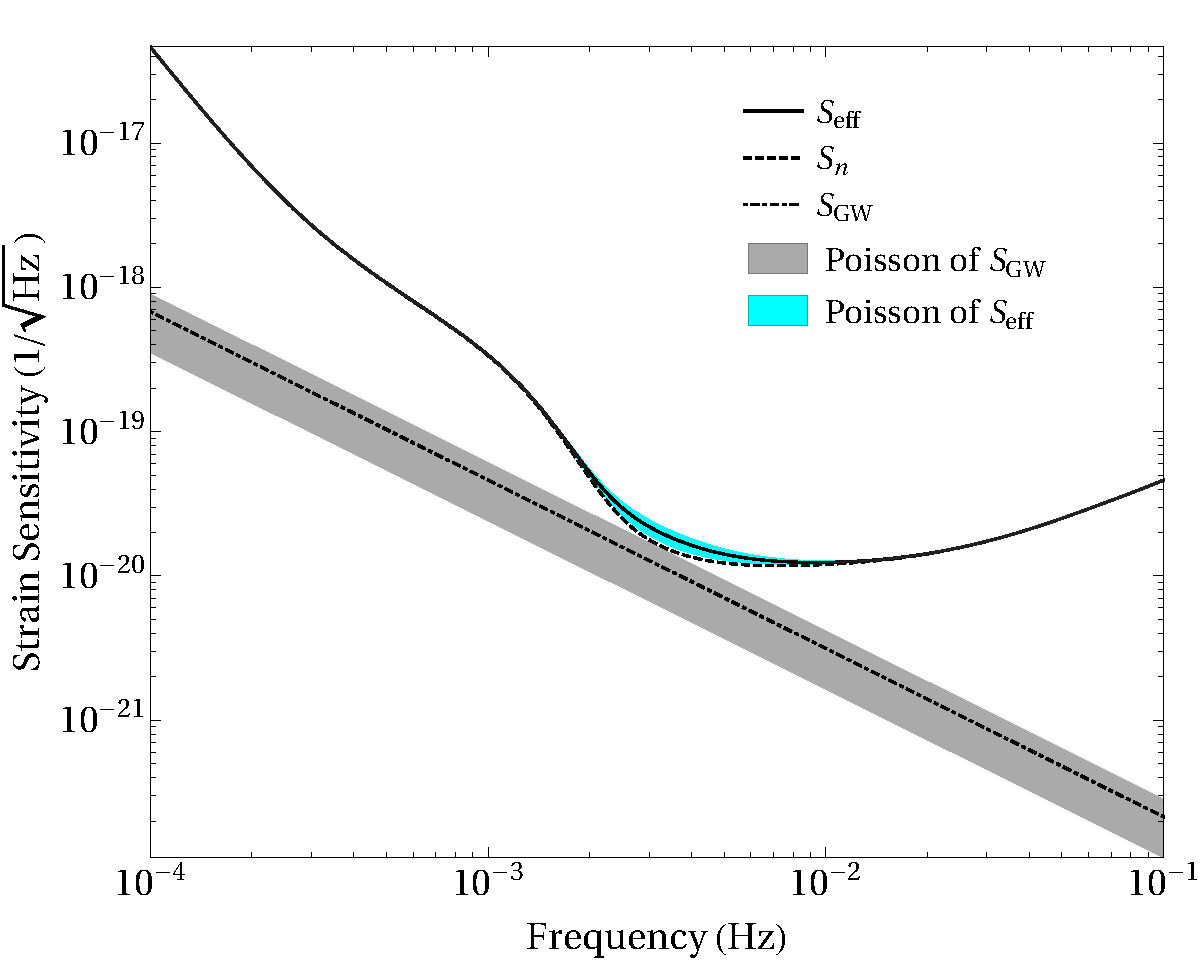
\includegraphics[width=\textwidth]{lisa-sensitivity-PBH-power.pdf}
    \bicaption{\label{lisa-sensitivity-PBH-power}
        由原初双黑洞和双中子星产生的总的随机引力波背景导致LISA探测器的有效应变灵敏度$S_{\mathrm{eff}}$(黑色实线)以及相应的泊松误差(青色区域)。原初黑洞的质量函数为幂率形式。图中还给出了LISA探测器的应变灵敏度$S_n$(虚线)以及引力波背景对应的应变灵敏度$S_{\mathrm{GW}}$(点虚线)和相应的泊松误差(灰色区域)。
    }{The effective strain sensitivity $S_{\mathrm{eff}}$ (black solid curve) of LISA
        and its Poisson uncertainties (cyan region),
        due to the effect of the total stochastic gravitational-wave background from primordial-origin binary black holes 
        (with a \textit{power-law} mass function) and binary neutron stars.
        We also show LISA's strain sensitivity $S_n$ (dashed curve),
        and $S_{\mathrm{GW}}$ (dot-dashed curve) 
        along with its Poisson uncertainties (grey shaded region).}
\end{figure}  

\begin{figure}[htbp!]
    \centering
    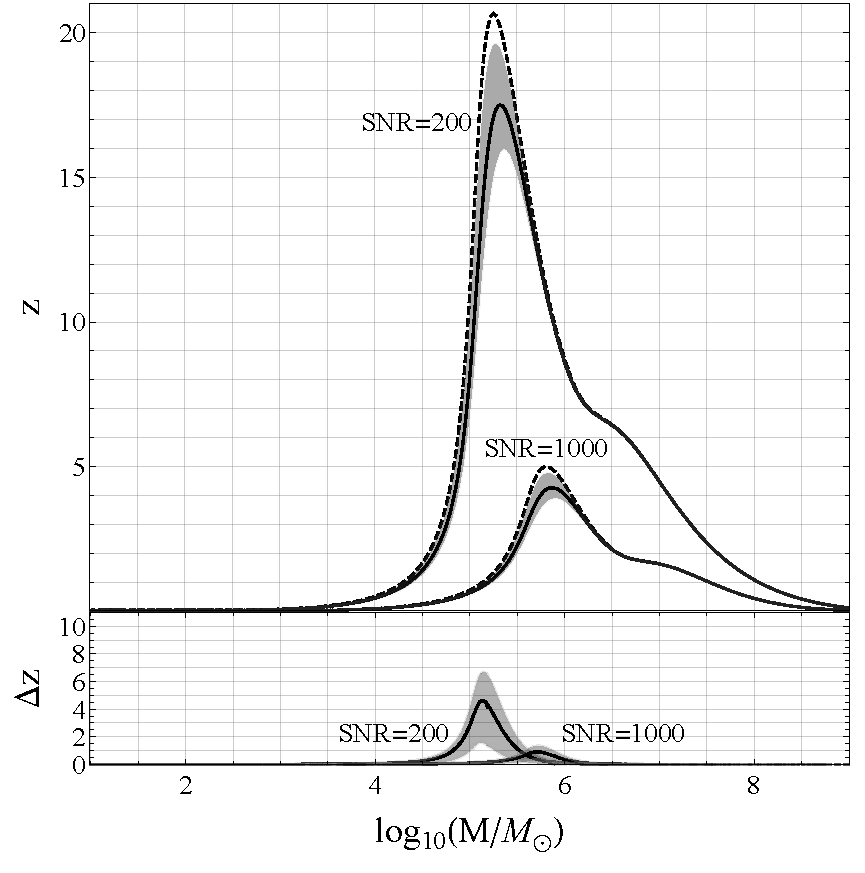
\includegraphics[width=\textwidth]{z-PBH-power.pdf}
    \bicaption[由原初双黑洞和双中子星产生的总的随机引力波背景对LISA探测器对于大质量双黑洞系统最大可探测红移$z$的影响。我们用$M$表示大质量双黑洞的总质量。原初黑洞的质量函数为幂率形式。我们固定质量比为$q=0.2$。我们分别考虑$\SNR=200$和$\SNR=1000$的两种情况。上图的虚线表示LISA最大可探测红移的等高线,而黑色实线表示考虑了随机引力波背景后LISA的最大可探测红移的等高线。灰色区域是黑色实线对应的泊松误差范围。下图给出了考虑随机引力波背景后对LISA最大可探测红移所引起的变化及误差范围。]{\label{z-PBH-power}
        由原初双黑洞和双中子星产生的总的随机引力波背景对LISA探测器对于大质量双黑洞系统最大可探测红移$z$的影响。我们用$M$表示大质量双黑洞的总质量。原初黑洞的质量函数为幂率形式。仿照\cite{Audley:2017drz},我们固定质量比为$q=0.2$。我们分别考虑$\SNR=200$和$\SNR=1000$的两种情况。上图的虚线表示LISA最大可探测红移的等高线,而黑色实线表示考虑了随机引力波背景后LISA的最大可探测红移的等高线。灰色区域是黑色实线对应的泊松误差范围。下图给出了考虑随机引力波背景后对LISA最大可探测红移所引起的变化及误差范围。
    }{The impacts of the total stochastic gravitational-wave background from primordial-origin binary black holes 
        (with a \textit{power-law} mass function) and binary neutron stars, 
        on the largest detectable redshift $z$ of MBHB (with total mass $M$) coalescences for LISA.
        The mass ratio is set to $q=0.2$ following \cite{Audley:2017drz}. 
        The upper panel shows the contours of $\SNR=200$ and $\SNR=1000$ 
        for LISA (dashed curves), 
        together with the effect of stochastic gravitational-wave background (black curves) and the Poisson error 
        bars (grey shaded region). 
        The lower panel shows the residuals of corresponding contours. }
\end{figure}

利用LIGO第一个观测阶段探测到的$3$个双黑洞并合事件,并考虑选择效应后,我们得到$\al$的最佳拟合值为$\al = 1.61$。固定$\al$的大小为其最佳拟合值,我们进而得到局域并合率$R$的中心值以及$90\%$的置信区间为$R = 80\,^{+108}_{-56}$\, $\gpcyr$。在\Fig{posterior-PBH-power}中,我们给出了$\al$和$R$的后验分布。从局域并合率$R$的后验分布,我们进一步得到原初黑洞占冷暗物质的丰度为$\fpbh = 3.8\,^{+2.3}_{-1.8} \times 10^{-3}$。我们的结果和之前的估算是一致的,即$10^{-3} \lesssim \fpbh \lesssim 10^{-2}$\citep{Sasaki:2016jop,Ali-Haimoud:2017rtz,Raidal:2017mfl,    Kocsis:2017yty,Chen:2018czv},从而验证了主要的冷暗物质不是由恒星级质量的原初黑洞构成的。



利用\Eq{OmegaGW},我们可以计算相应的随机引力波背景。\Fig{OmegaGW-PBH-power}给出了随机引力波背景的无量纲能量密度谱。从图上可以看出,随机引力波背景的强度可以超过LIGO设计阶段和LISA对应的灵敏度曲线,表明原初双黑洞和双中子星产生的随机引力波背景可以被LIGO设计阶段和LISA探测到。

在LIGO和LISA的可探测频段内,具有幂率质量分布的原初双黑洞和双中子星产生的引力波背景都近似和频率的$2/3$次方成正比,即$\ogw \propto \nu^{2/3}$。这是因为在可探测的频段内,随机引力波背景的贡献主要来自于双黑洞或双中子星的旋进阶段,而在旋进阶段,单个双黑洞或双中子星辐射的引力波能量谱大概就和频率的$2/3$次方成正比。在\Table{Omegaf-PBH-power}中,我们总结了在LIGO和LISA最灵敏的频率附近的随机引力波背景的能量密度的大小$\ogw (\nu)$。


\Fig{SNR-PBH-power}给出了预期累积信噪比关于时间的函数关系。由图可知,在观测$2$小时后,LISA可以探测到来自具有幂率质量分布的原初双黑洞和双中子星的中心值大小的随机引力波背景,相应的信噪比为$\mathrm{SNR} = 5$。在最乐观的情况下LISA观测$2$个小时就能探测到信噪比$\mathrm{SNR} = 5$的总的随机引力波背景,而在最悲观的情况下LISA观测$5$天能探测到信噪比$\mathrm{SNR} = 5$的总的随机引力波背景。


\Fig{lisa-sensitivity-PBH-power}给出了应变灵敏度曲线。\Fig{z-PBH-power}给出了随机引力波背景对LISA探测大质量双黑洞并合的信噪比的影响,表明最大可探测红移会由于未解析出来的随机引力波背景的影响而减小。这也表明LISA可探测的区域被压低了,从而减少LISA可探测到的大质量双黑洞并合的事件数。从\Fig{z-PBH-power}看出,由于随机引力波背景导致的等效噪音可以压低LISA对$10^5 \Msun$以上的种子黑洞并合的最大可探测红移。




\FloatBarrier
%%%%%%%%%%%%%%%%%%%%%%%%%%%%%%%%%%%%%%%%%%%%%%%%%%%%%%%%%%%%%%%%%%%%%%
\subsection{对数正态质量函数}

我们现在考虑对数正态的原初黑洞质量分布\citep{Dolgov:1992pu},
\e\label{log}
P(m) = \frac{1}{\sqrt{2 \pi} \s m} 
\exp\(-\frac{\ln^2(m/m_c)}{2 \s^2}\),
\q
其中$m_c$表征质量谱的峰值,而$\s$表征质量谱的宽度。在这种情况下,模型有三个自由参数,为$\{\vth, R\} = \{m_c, \s, R\}$.

\begin{figure}[htb!]
    \centering
    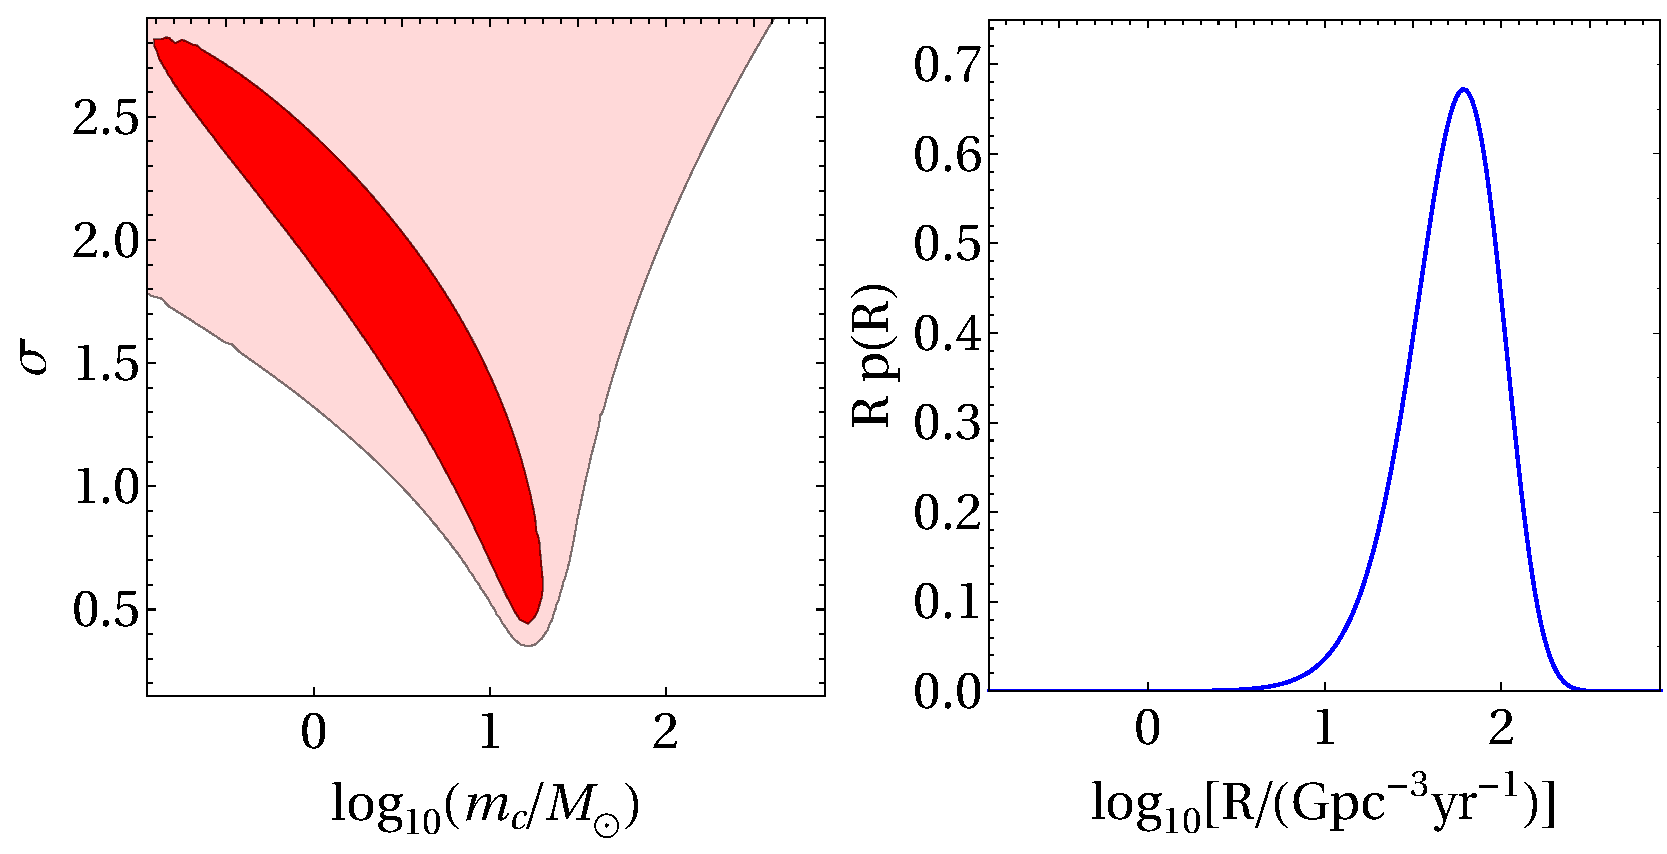
\includegraphics[width=\textwidth]{posterior-PBH-log.pdf}
    \bicaption{\label{posterior-PBH-log} 
        当原初黑洞质量函数为\textit{对数正态}形式的情况下,用LIGO第一个观测阶段的$3$个双黑洞并合事件拟合得到模型参数$\{\vth, R\} = \{m_c, \s, R\}$的一维和二维后验分布。左图的等高线分别对应$68\%$和$95\%$的置信区间。
    }{The posterior distributions for $\{\vth, R\} = \{m_c, \s, R\}$ of
    \textit{lognormal} mass function for primordial black holes, at the $68\%$ and $95\%$ 
    credible level, respectively, by using $3$ events from 
    LIGO's O1 observing run.  }
\end{figure}

利用LIGO第一个观测阶段探测到的$3$个双黑洞并合事件,并考虑选择效应后,我们得到$m_c$和$\s$的最佳拟合值为$\{m_c, \s\} = \{14.8 \Msun, 0.65\}$。固定$m_c$和$\s$的大小为其最佳拟合值,我们进而得到局域并合率$R$的中心值以及$90\%$的置信区间为$R = 55\,^{+74}_{-38}$\, $\gpcyr$。在\Fig{posterior-PBH-log}中,我们给出了$m_c$、$\s$和$R$的后验分布。从局域并合率$R$的后验分布,我们进一步得到原初黑洞占冷暗物质的丰度为$\fpbh = 2.8\,^{+1.6}_{-1.3} \times 10^{-3}$。我们的结果和之前的估算是一致的,即$10^{-3} \lesssim \fpbh \lesssim 10^{-2}$\citep{Sasaki:2016jop,Ali-Haimoud:2017rtz,Raidal:2017mfl,    Kocsis:2017yty,Chen:2018czv},从而验证了主要的冷暗物质不是由恒星级质量的原初黑洞构成的。

\begin{figure}[htbp!]
    \centering
    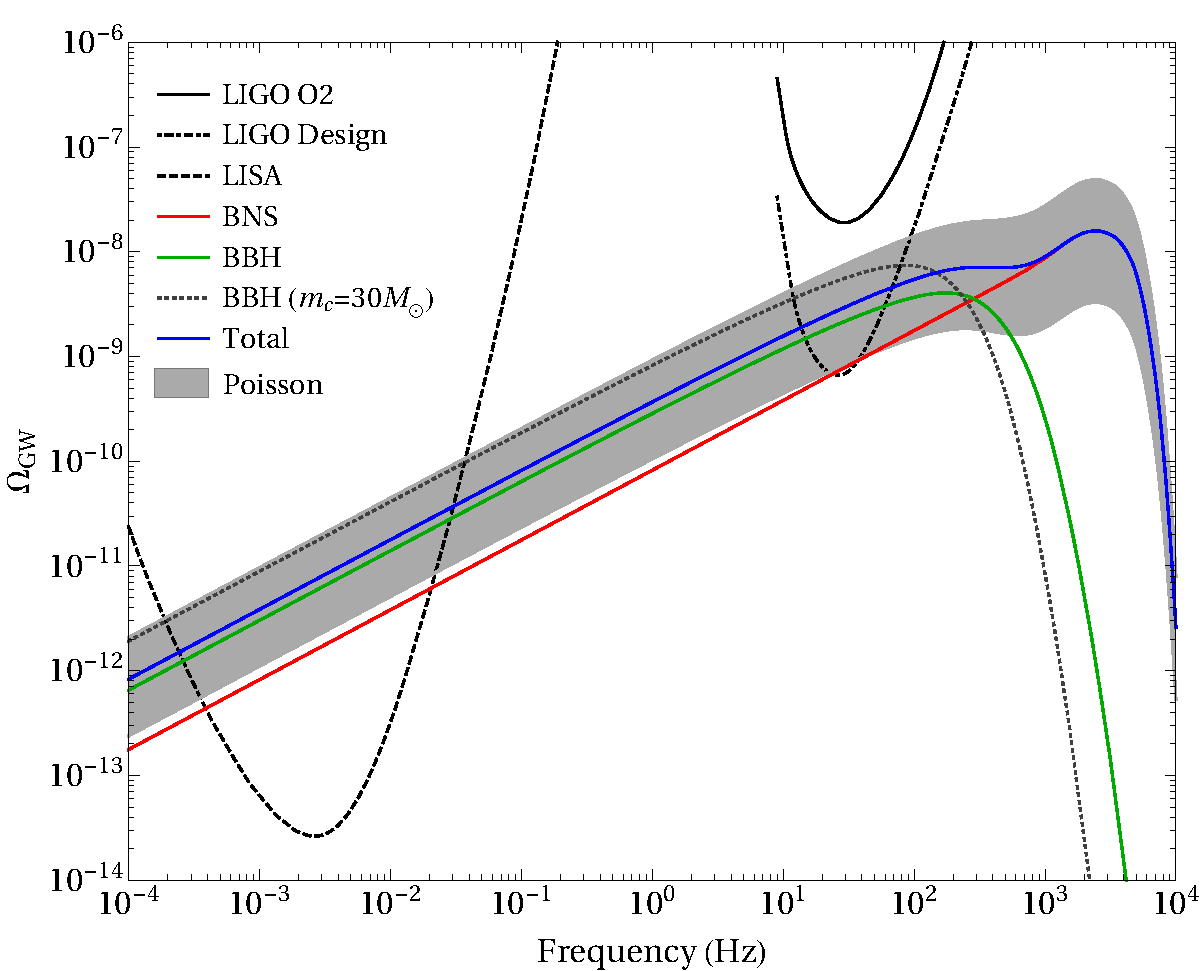
\includegraphics[width=0.8\textwidth]{OmegaGW-PBH-log.pdf}
    \bicaption[来自对数正态质量分布的原初双黑洞和双中子星产生的随机引力波背景。绿线是双黑洞对应的随机引力波背景,而红线是双中子星对应的随机引力波背景。蓝色表示总的引力波背景;灰色区域则表示总的随机引力波背景的泊松误差。对于双黑洞,我们固定$\{m_c, \s\}$和局域并合率$R$为其最佳拟合值,即$\{m_c, \s\} = \{14.8\, \Msun,\,0.65\}$和$R = 55\,^{+74}_{-38}$\, $\gpcyr$。该情况下对应的原初黑洞占冷暗物质的丰度为$\fpbh = 2.8\,^{+1.6}_{-1.3} \times 10^{-3}$;而对于双中子星,我们取局域并合率为$R = 1540_{-1220}^{+3200}$\,$\gpcyr$。图中的黑色实线表示LIGO第二个观测阶段(O2)的幂率积分曲线;点虚线表示LIGO设计阶段对应的幂率积分曲线;而虚线则表示LISA观测四年对应的幂率积分曲线。LIGO设计阶段和LISA对应的幂率积分曲线都能跨过泊松误差区域,表明原初双黑洞和双中子星产生的随机引力波背景可以被LIGO设计阶段和LISA探测到。]{\label{OmegaGW-PBH-log} 
        来自对数正态质量分布的原初双黑洞和双中子星产生的随机引力波背景。绿线是双黑洞对应的随机引力波背景,而红线是双中子星对应的随机引力波背景。蓝色表示总的引力波背景;灰色区域则表示总的随机引力波背景的泊松误差。对于双黑洞,我们固定$\{m_c, \s\}$和局域并合率$R$为其最佳拟合值,即$\{m_c, \s\} = \{14.8\, \Msun,\,0.65\}$和$R = 55\,^{+74}_{-38}$\, $\gpcyr$,且$\fpbh = 2.8\,^{+1.6}_{-1.3} \times 10^{-3}$;而对于双中子星,我们取局域并合率为$R = 1540_{-1220}^{+3200}$\,$\gpcyr$\citep{TheLIGOScientific:2017qsa}。图中的黑色实线表示LIGO第二个观测阶段(O2)的幂率积分曲线;点虚线表示LIGO设计阶段对应的幂率积分曲线;而虚线则表示LISA观测四年对应的幂率积分曲线。LIGO设计阶段和LISA对应的幂率积分曲线都能跨过泊松误差区域,表明原初双黑洞和双中子星产生的随机引力波背景可以被LIGO设计阶段和LISA探测到。
    }{The predicted stochastic gravitational-wave background from the binary neutron stars and primordial-origin binary black holes
    with a \textit{lognormal} mass function. 
    The red and green curves are backgrounds from the binary neutron stars (BNSs) and binary black holes (BBHs), respectively. 
    The total background is shown in the blue curve, while
    its Poisson error bars are in the grey shaded region.
    For binary black holes, we adopt the best-fit values for 
    $\{m_c, \s\} = \{14.8\, \Msun,\,0.65\}$, 
    and the inferred local merger rate $R = 55\,^{+74}_{-38}$\, $\gpcyr$,
    which corresponds to $\fpbh = 2.8\,^{+1.6}_{-1.3} \times 10^{-3}$.
    And for binary neutron stars, we adopt $R = 1540_{-1220}^{+3200}$\,$\gpcyr$ 
    \citep{TheLIGOScientific:2017qsa}.
    The dotted line shows the background from binary black holes with $m_c = 30 \Msun$, 
    by fixing $\s = 0.65$ and $R = 55$\, $\gpcyr$.
    We also show the expected PI curves for LISA with $4$ years of 
    observation (dashed) and
    LIGO's O2 (black) and design sensitivity (dot-dashed).
    The PI curves for LISA and LIGO's design sensitivity cross the Poisson
    error region, indicating the possibility to detect this background.}
\end{figure}

\begin{table}[htb!]
    \centering
    \begin{tabular}{c|c|c}
        &\ $\Omega_{\mathrm{GW}}(25 \, \mathrm{Hz})$ \
        &\ $\Omega_{\mathrm{GW}}(3 \times 10^{-3} \, \mathrm{Hz})$\,\\
        \hline
        BNS\, &  $0.7^{+1.5}_{-0.6} \times 10^{-9}$ 
        & $1.7^{+3.5}_{-1.4} \times 10^{-12}$ \\
        [.3em]
        \hline
        BBH\, & $2.0^{+2.7}_{-1.4} \times 10^{-9}$  
        & $6.3^{+8.5}_{-4.2} \times 10^{-12}$ \\
        [.3em]
        \hline
        Total\, & $2.7^{+4.2}_{-2.0} \times 10^{-9}$  
        & $8.0^{+12}_{-5.6} \times 10^{-12}$ \\
        [.2em]
    \end{tabular}
    \bicaption{\label{Omegaf-PBH-log}
        原初双黑洞产生的随机引力波背景、双中子星产生的随机引力波背景以及总的随机引力波背景在LIGO和LISA最灵敏的频率附近(分别为$25 \, \mathrm{Hz}$和$3 \times 10^{-3} \, \mathrm{Hz}$)的大小。原初黑洞质量函数为对数正态形式。我们还给出了$90\%$的泊松误差范围。
    }{Estimates of the background energy density $\ogw (\nu)$ at the most sensitive frequencies of LIGO (near $25$ Hz) and LISA (near $3\times 10^{-3}$ Hz) for each of the binary neutron star (BNS), primordial-origin binary black hole (BBH, with a \textit{lognormal} mass function) and total background contributions, along with the $90\%$ Poisson error bounds.}
\end{table}

\begin{figure}[htbp!]
    \centering
    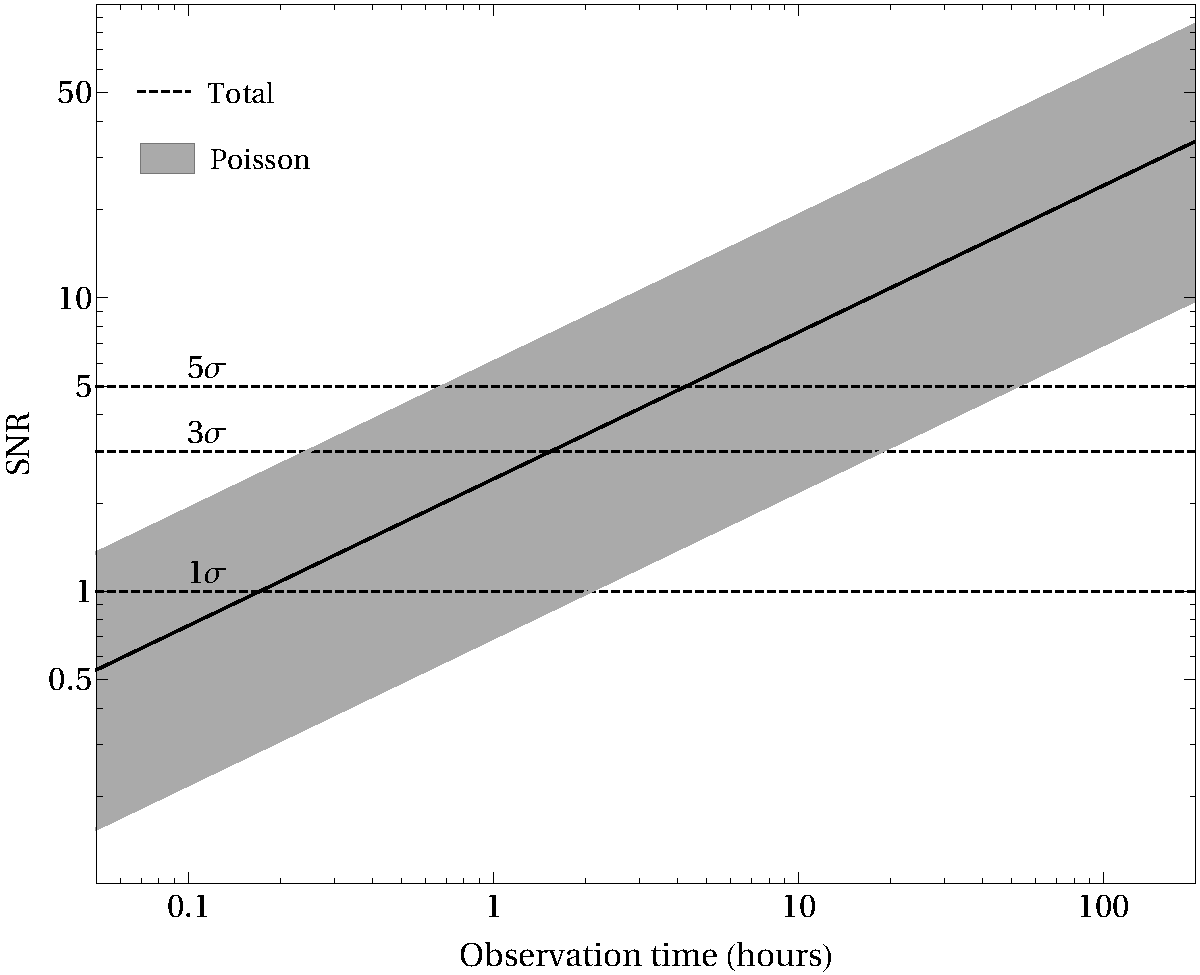
\includegraphics[width=\textwidth]{SNR-PBH-log.pdf}
    \bicaption[LISA探测器对探测原初双黑洞和双中子星产生的总的随机引力波背景的信噪比随观测时间的关系。原初黑洞质量函数为对数正态形式。黑色实线表示信噪比的中心值,而灰色区域表示信噪比的误差范围。对于双黑洞,我们固定$\{m_c, \s\}$和局域并合率$R$为其最佳拟合值,即$\{m_c, \s\} = \{14.8\, \Msun,\,0.65\}$和$R = 55\,^{+74}_{-38}$\, $\gpcyr$。该情况下对应的原初黑洞占冷暗物质的丰度为$\fpbh = 2.8\,^{+1.6}_{-1.3} \times 10^{-3}$;而对于双中子星,我们取局域并合率为$R = 1540_{-1220}^{+3200}$\,$\gpcyr$。在大约观测$5$个小时后,LISA可以探测到中心值大小的总的随机引力波背景;探测的信噪比为$\mathrm{SNR}=5$。]{\label{SNR-PBH-log} 
        LISA探测器对探测原初双黑洞和双中子星产生的总的随机引力波背景的信噪比随观测时间的关系。原初黑洞质量函数为对数正态形式。黑色实线表示信噪比的中心值,而灰色区域表示信噪比的误差范围。对于双黑洞,我们固定$\{m_c, \s\}$和局域并合率$R$为其最佳拟合值,即$\{m_c, \s\} = \{14.8\, \Msun,\,0.65\}$和$R = 55\,^{+74}_{-38}$\, $\gpcyr$。该情况下对应的原初黑洞占冷暗物质的丰度为$\fpbh = 2.8\,^{+1.6}_{-1.3} \times 10^{-3}$;而对于双中子星,我们取局域并合率为$R = 1540_{-1220}^{+3200}$\,$\gpcyr$\citep{TheLIGOScientific:2017qsa}。在大约观测$5$个小时后,LISA可以探测到中心值大小的总的随机引力波背景;探测的信噪比为$\mathrm{SNR}=5$。
    }{The SNR of LISA as a function of observation time for median total 
    stochastic gravitational-wave background (black curve) and associated uncertainties (grey shaded region),
    from primordial-origin binary black holes (with a \textit{lognormal} mass function) and binary neutron stars.
    Here, we adopt the best-fit values for 
    $\{m_c, \s\} = \{14.8\, \Msun,\,0.65\}$, 
    and the inferred local merger rate $R = 55\,^{+74}_{-38}$\, $\gpcyr$,
    which corresponds to $\fpbh = 2.8\,^{+1.6}_{-1.3} \times 10^{-3}$.
    The predicted median total background can be detected with 
    $\mathrm{SNR}=5$ after about $5$ hours of observation time.}
\end{figure}

利用\Eq{OmegaGW},我们可以计算相应的随机引力波背景。\Fig{OmegaGW-PBH-log}给出了随机引力波背景的无量纲能量密度谱。从图上可以看出,随机引力波背景的强度可以超过LIGO设计阶段和LISA对应的灵敏度曲线,表明原初双黑洞和双中子星产生的随机引力波背景可以被LIGO设计阶段和LISA探测到。

在LIGO和LISA的可探测频段内,具有对数正态质量分布的原初双黑洞和双中子星产生的引力波背景都近似和频率的$2/3$次方成正比,即$\ogw \propto \nu^{2/3}$。这是因为在可探测的频段内,随机引力波背景的贡献主要来自于双黑洞或双中子星的旋进阶段,而在旋进阶段,单个双黑洞或双中子星辐射的引力波能量谱大概就和频率的$2/3$次方成正比。在\Table{Omegaf-PBH-log}中,我们总结了在LIGO和LISA最灵敏的频率附近的随机引力波背景的能量密度的大小$\ogw (\nu)$。



\begin{figure}[htbp!]
    \centering
    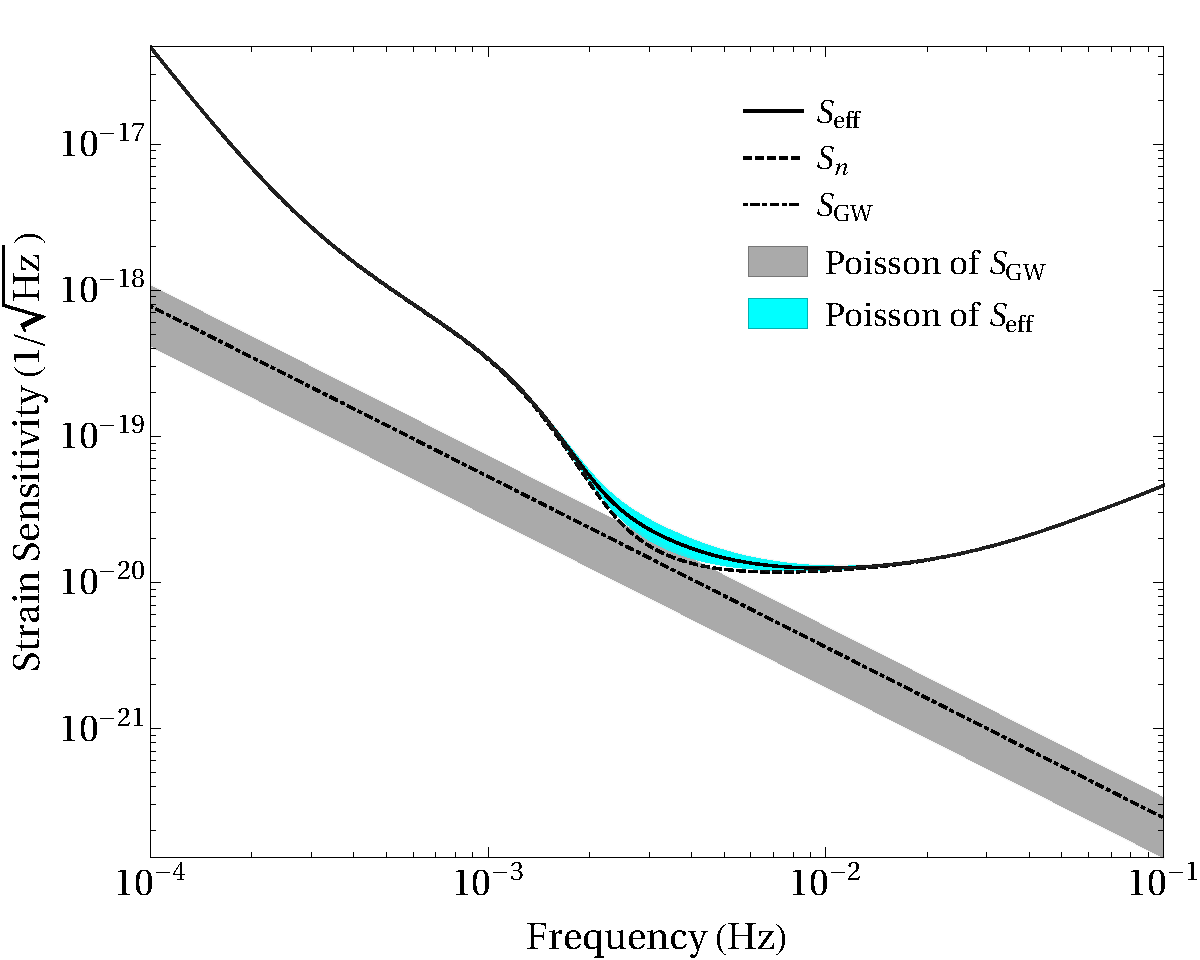
\includegraphics[width=\textwidth]{lisa-sensitivity-PBH-log.pdf}
    \bicaption{\label{lisa-sensitivity-PBH-log}        
        由原初双黑洞和双中子星产生的总的随机引力波背景导致LISA探测器的有效应变灵敏度$S_{\mathrm{eff}}$(黑色实线)以及相应的泊松误差(青色区域)。原初黑洞质量函数为对数正态形式。图中还给出了LISA探测器的应变灵敏度$S_n$(虚线)以及引力波背景对应的应变灵敏度$S_{\mathrm{GW}}$(点虚线)和相应的泊松误差(灰色区域)。
    }{The effective strain sensitivity $S_{\mathrm{eff}}$ (black solid curve) of LISA
    and its Poisson uncertainties (cyan region),
    due to the effect of the total stochastic gravitational-wave background from primordial-origin binary black holes 
    (with a \textit{log-normal} mass function) and binary neutron stars.
    We also show LISA's strain sensitivity $S_n$ (dashed curve),
    and $S_{\mathrm{GW}}$ (dot-dashed curve) 
    along with its Poisson uncertainties (grey shaded region).}
\end{figure}  



\begin{figure}[htbp!]
    \centering
    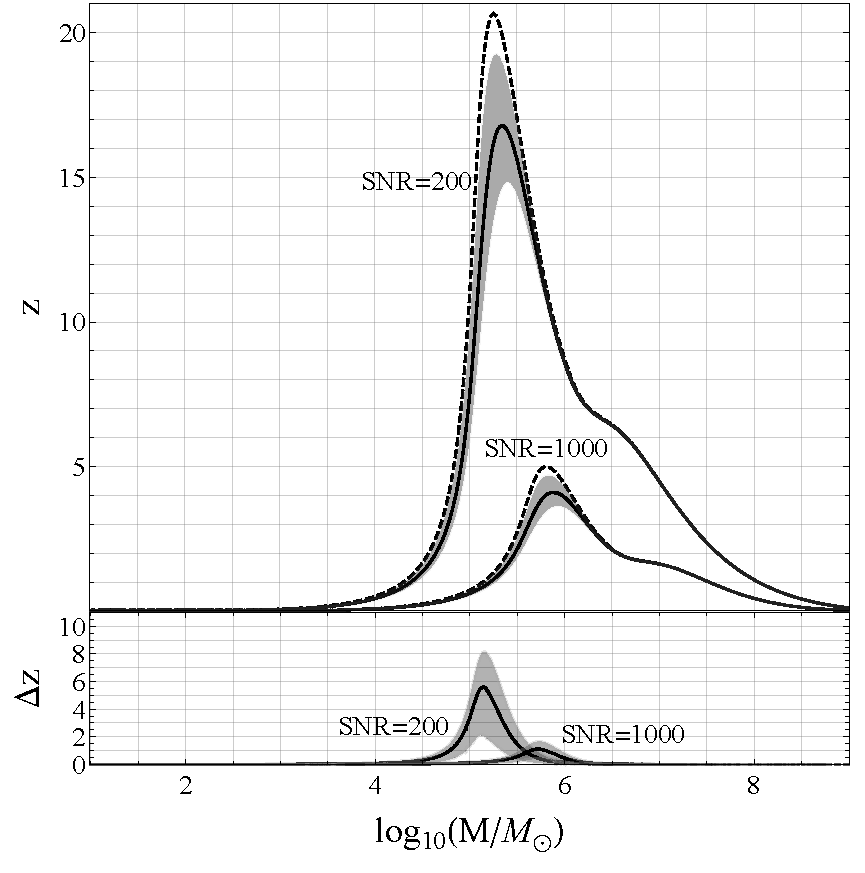
\includegraphics[width=\textwidth]{z-PBH-log.pdf}
    \bicaption[由原初双黑洞和双中子星产生的总的随机引力波背景对LISA探测器对于大质量双黑洞系统最大可探测红移$z$的影响。我们用$M$表示大质量双黑洞的总质量。原初黑洞质量函数为对数正态形式。仿照,我们固定质量比为$q=0.2$。我们分别考虑$\SNR=200$和$\SNR=1000$的两种情况。上图的虚线表示LISA最大可探测红移的等高线,而黑色实线表示考虑了随机引力波背景后LISA的最大可探测红移的等高线。灰色区域是黑色实线对应的泊松误差范围。下图给出了考虑随机引力波背景后对LISA最大可探测红移所引起的变化及误差范围。]{\label{z-PBH-log}
        由原初双黑洞和双中子星产生的总的随机引力波背景对LISA探测器对于大质量双黑洞系统最大可探测红移$z$的影响。我们用$M$表示大质量双黑洞的总质量。原初黑洞质量函数为对数正态形式。仿照\cite{Audley:2017drz},我们固定质量比为$q=0.2$。我们分别考虑$\SNR=200$和$\SNR=1000$的两种情况。上图的虚线表示LISA最大可探测红移的等高线,而黑色实线表示考虑了随机引力波背景后LISA的最大可探测红移的等高线。灰色区域是黑色实线对应的泊松误差范围。下图给出了考虑随机引力波背景后对LISA最大可探测红移所引起的变化及误差范围。
    }{The impacts of the total stochastic gravitational-wave background from primordial-origin binary black holes 
    (with a \textit{lognormal} mass function) and binary neutron stars, 
    on the largest detectable redshift $z$ of MBHB (with total mass $M$) coalescences for LISA.
    The mass ratio is set to $q=0.2$ following \cite{Audley:2017drz}. 
    The upper panel shows the contours of $\SNR=200$ and $\SNR=1000$ 
    for LISA (dashed curves), 
    together with the effect of stochastic gravitational-wave background (black curves) and the Poisson error 
    bars (grey shaded region). 
    The lower panel shows the residuals of corresponding contours. }
\end{figure}


\Fig{SNR-PBH-log}给出了预期累积信噪比关于时间的函数关系。由图可知,在观测$5$小时后,LISA可以探测到来自具有对数正态质量分布的原初双黑洞和双中子星的中心值大小的随机引力波背景,相应的信噪比为$\mathrm{SNR} = 5$。在最乐观的情况下LISA观测$1$个小时就能探测到信噪比$\mathrm{SNR} = 5$的总的随机引力波背景,而在最悲观的情况下LISA观测$3$天能探测到信噪比$\mathrm{SNR} = 5$的总的随机引力波背景。

\Fig{lisa-sensitivity-PBH-log}给出了应变灵敏度曲线。\Fig{z-PBH-log}给出了随机引力波背景对LISA探测大质量双黑洞并合的信噪比的影响,表明最大可探测红移会由于未解析出来的随机引力波背景的影响而减小。这也表明LISA可探测的区域被压低了,从而减少LISA可探测到的大质量双黑洞并合的事件数。从\Fig{z-PBH-log}看出,由于随机引力波背景导致的等效噪音可以压低LISA对$10^5 \Msun$以上的种子黑洞并合的最大可探测红移。



%%%%%%%%%%%%%%%%%%%%%%%%%%%%%%%%%%%%%%%%%%%%%%%%%%%%%%%%%%%%%%%%%%%%%%
\section{总结和讨论}

在本章中,我们计算了来自双黑洞和双中子星并合产生的随机引力波背景。而且探究了这一随机引力波背景对LISA空间引力波探测器探测能力的影响。我们考虑了两种不同的双黑洞形成机制,分别是天体物理双黑洞和原初双黑洞机制。

对于天体物理黑洞,我们采用了被广泛接受的``\textit{Vangioni}"模型\citep{Dvorkin:2016wac}。而对于原初黑洞,我们考虑了两种流行的迥异的原初黑洞质量谱,分别为幂率质量分布和对数正态质量分布。对于幂率质量谱的情况,我们从LIGO的引力波数据分析得到局域并合率为$R = 80\,^{+108}_{-56}$\, $\gpcyr$,相应的原初黑洞占冷暗物质的丰度为$\fpbh = 3.8\,^{+2.3}_{-1.8} \times 10^{-3}$。对于对数正态的质量谱,我们得到$R = 55\,^{+74}_{-38}$\, $\gpcyr$,对应于$\fpbh = 2.8\,^{+1.6}_{-1.3} \times 10^{-3}$。由于幂率形式的质量谱会给出更多的轻质量的原初黑洞,所以相较对数正态质量分布而言,为了和\lvc 相自洽,其预言的局域并合率要大一些。之前文献\citep{Kawasaki:2016jop,Ali-Haimoud:2017rtz,Raidal:2017mfl,Kocsis:2017yty,Chen:2018czv}中对原初黑洞占冷暗物质的估计大约为$10^{-3} \lesssim \fpbh \lesssim 10^{-2}$。对于这两种原初黑洞的质量谱,我们推断得到的原初黑洞的丰度和之前的估计一致的,从而验证了主要的冷暗物质不是由恒星级质量的原初黑洞构成的。

我们发现原初双黑洞产生的随机引力波背景要比天体物理双黑洞产生的随机引力波背景要强(见\Fig{OmegaGW-sBH}、\Fig{OmegaGW-PBH-power}、\Fig{OmegaGW-PBH-log}以及\Table{Omegaf-sBH}、\Table{Omegaf-PBH-power}、\Table{Omegaf-PBH-log})。这是由于原初双黑洞和天体物理双黑洞的并合率随黑洞的质量和红移的关系不同导致的。特别是,原初双黑洞的并合率会随着红移的增长而快速增长;而天体物理双黑洞的并合率则随着红移先增长,接着在红移为$z \sim 1-2$附近达到峰值,然后急剧速减小。我们还发现,在\lvc 和LISA灵敏的频段内,不管是天体物理双黑洞还是原初双黑洞形成的随机引力波背景的能量密度谱都和频率成$2/3$次方的关系,即$\ogw \propto \nu^{2/3}$。所以用\lvc 和LISA通过探测随机引力波背景的方法将很难区分到底是是天体物理双黑洞还是原初双黑洞形成的随机引力波背景。

最后,我们发现由双黑洞和双中子星形成的总的随机引力波背景很可能被未来的引力波探测器\lvc 和LISA探测到(见\Fig{OmegaGW-sBH}、\Fig{SNR-sBH}、\Fig{OmegaGW-PBH-power}、\Fig{SNR-PBH-power}、\Fig{OmegaGW-PBH-log}、\Fig{SNR-PBH-log})。这些随机引力波背景如果不从噪音背景中扣除掉的话,会成为LISA的额外噪音源(见\Fig{lisa-sensitivity-sBH}、\Fig{lisa-sensitivity-PBH-power}、\Fig{lisa-sensitivity-PBH-log}),从而弱化LISA的探测能力。例如,探测大质量双黑洞的并合是LISA的一个关键科学目标。由于随机引力波背景的影响,会压低LISA对于大质量双黑洞的最大可探测红移(见\Fig{z-sBH}、\Fig{z-PBH-power}、\Fig{z-PBH-log})。所以,为了提高探测器的探测能力,需要将随机引力波背景从LISA的噪音中扣除掉。
\chapter{区分原初黑洞和天体物理黑洞}\label{chap:distinguish}

%We investigate how the next generation gravitational-wave (引力波) detectors, such as Einstein Telescope (ET) and Cosmic Explorer (CE), can be used to distinguish primordial black holes (原初黑洞) from astrophysical black holes (ABHs). Since a direct detection of sub-solar mass black holes can be taken as the smoking gun for 原初黑洞, we estimate the detectable limits of the abundance of sub-solar mass 原初黑洞 in cold dark matter by the targeted search for sub-solar mass 原初黑洞 binaries and binaries containing a sub-solar mass 原初黑洞 and a super-solar mass 原初黑洞, respectively. On the other hand, according to the different redshift evolutions of the merger rate for 原初黑洞 binaries and 天体物理黑洞 binaries, we forecast the detectable event rate distributions for the 原初黑洞 binaries and 天体物理黑洞 binaries by ET and CE respectively, which can serve as a method to distinguish super-solar mass 原初黑洞 from ABHs.

\section{背景介绍}
根据\lvc 科学组织最新发布的引力波瞬变目录2~\cite{Abbott:2020niy},目前一共探测到了50个致密双星并合事例。其中大多数都是双黑洞并合的事例。探测到了这么多双黑洞并合的引力波事件,加深了人类对宇宙的认识,但是还有很多问题需要回答。例如,这些双黑洞到底是如何形成和演化的,目前还是一个被广泛探讨的话题\cite{Bird:2016dcv,Sasaki:2016jop,Chen:2018czv,Clesse:2017bsw,Fishbach:2017dwv,Clesse:2016vqa,Antonini:2016gqe,Inayoshi:2017mrs,Ali-Haimoud:2017rtz,Perna:2019axr,Kavanagh:2018ggo,Rodriguez:2015oxa,Rodriguez:2016kxx,Park:2017zgj,Wu:2020drm,Belczynski:2014iua,Belczynski:2016obo,Woosley:2016nnw,Rodriguez:2018rmd,Choksi:2018jnq,2010AIPC.1314..291D,deMink:2016vkw}。

在引力波被探测到之前,由X射线观测到的黑洞的质量通常比较小\cite{Wiktorowicz:2013dua,Casares:2013tpa,Corral-Santana:2013uua,Corral-Santana:2015fud}。然而引力波观测到的双黑洞的质量要比X射线观测到的黑洞的质量要重很多。这一事实不禁让人们猜想观测到的双黑洞并合可能起源于恒星质量的原初黑洞\cite{Bird:2016dcv,Sasaki:2016jop,Chen:2018czv,Clesse:2017bsw}。原初黑洞是在早期宇宙中由原初密度扰动的引力塌缩而形成的黑洞\cite{Hawking:1971ei,Carr:1974nx,Khlopov:2008qy,Sasaki:2018dmp}。其与起源于大质量恒星死亡而形成的天体物理黑洞经历了完全不同的演化历史。原初黑洞可能会构成部分的冷暗物质。而原初黑洞占冷暗物质的丰度,即$\fpbh$,已经受到了各种实验,例如星系外伽马射线\cite{Carr:2009jm}、伽马射线暴的femtolensing\cite{Barnacka:2012bm}、本星系中的白矮星\cite{Graham:2015apa}、Subaru/HSC微透镜\cite{Niikura:2017zjd}、开普勒毫-微透镜\cite{Griest:2013esa}、OGLE微透镜\cite{Niikura:2019kqi}、EROS/MACHO微透镜\cite{Tisserand:2006zx,Calcino:2018mwh}、超暗矮星系的动态加热\cite{Brandt:2016aco}、X射线/无线电\cite{Gaggero:2016dpq}、宇宙微波背景\cite{Ali-Haimoud:2016mbv,Blum:2016cjs,Horowitz:2016lib,Chen:2016pud,Poulin:2017bwe}以及引力波\cite{Wang:2016ana,Abbott:2018oah,Authors:2019qbw,Magee:2018opb,Wang:2019kaf,Chen:2019xse,Yuan:2019udt,Chen:2018rzo}等的限制。

除了原初黑洞模型,天体物理黑洞模型也可以解释\lvc 探测到的双黑洞。天体物理双黑洞的形成和并合是由演化环境主导的。在文献中,天体物理双黑洞模型主要有三种机制。第一种是\textit{动态形成}机制,即大质量恒星的演化形成黑洞,而黑洞被分离到星团核心,最后配对形成双黑洞系统\cite{Rodriguez:2015oxa,Rodriguez:2016kxx,Park:2017zgj}。第二种是\textit{经典孤立的双星演化}机制,即双黑洞是通过质量转移或公共包层抛射(common envelope ejection)而形成的\cite{Belczynski:2014iua,Belczynski:2016obo,Woosley:2016nnw,Rodriguez:2018rmd,Choksi:2018jnq}。第三种是\textit{化学均匀演化}机制,即由于氦气在整个包络体中的混合\cite{2010AIPC.1314..291D,deMink:2016vkw},使得恒星几乎在化学物质均匀的环境种演化形成黑洞。双黑洞的属性,如自旋\cite{Farr:2017uvj,Tiwari:2018qch,Ng:2018neg,Stevenson:2017dlk,Bogomazov:2018prw,Lopez:2018nkj,Sedda:2018nxm,Farr:2017gtv}、红移\cite{Fishbach:2018edt,Emami:2018taj,Bai:2018shq}和偏心率分布\cite{Samsing:2013kua,Samsing:2017xmd,Samsing:2017jnz,Lower:2018seu}等性质有可能区分不同机制的天体物理双黑洞模型。

在本节种,我们将探究通过使用引力波观测,特别是通过第三代地基引力波探测器,如爱因斯坦望远镜 (Einstein Telescope,简称ET)\cite{Punturo:2010zz}和宇宙勘探者(Cosmic Explorer,简称CE)\cite{Evans:2016mbw},来区分原初黑洞和天体物理黑洞的可能性。ET和CE有望每年探测到$\Od(10^5)$ \cite{Regimbau:2016ike,Vitale:2018yhm}个双黑洞并合事件,这个数目要远远大于比目前\lvc 探测到的双黑洞并合的数目。首先,我们考虑亚太阳质量($\lesssim 1\Msun$)的双黑洞。因为通常认为天体物理黑洞的质量要大于钱德勒赛卡质量极限($\sim 1.4 \Msun$)\cite{Chandrasekhar:1931ftj,Chandrasekhar:1931ih},所以直接探测到亚太阳质量的黑洞可以成为原初黑洞存在的关键证据。其次,我们考虑超太阳质量($\gtrsim 1\Msun$)的双黑洞。由于原初双黑洞和天体物理双黑洞的并合率随红移的演化可以有很大的不同,所以可探测双黑洞的事件数随红移的分布不同。我们分别估计ET和CE可探测到的原初黑洞和天体物理黑洞的事件数分布,这可以作为区分原初黑洞和天体物理黑洞的另一种方法。


%%%%%%%%%%%%%%%%%%%%%%%%%%%%%%%%%%%%%%%%%%%%%%%%%%%%%%%%%%%%%%%%%%%%%%%%%%%%%%%%
\section{\label{subsolar}通过亚太阳质量黑洞来区分原初黑洞和天体物理黑洞}
直接探测到亚太阳质量的黑洞可以作为原初黑洞的直接证据。可探测到的事件数不仅取决于原初双黑洞的并合率,而且还取决于引力波探测器的灵敏度。在下面的两个小节中,我们将分别考虑原初黑洞具有单色质量谱和一般质量谱的情况,来探讨不同的引力波探测器探测亚太阳质量黑洞的能力。

\subsection{\label{mono}原初黑洞具有单色质量谱的情况}
在本小节中,我们假设所有的原初黑洞都具有相同的质量,并通过对原初双黑洞的目标搜索(targeted search)来估计$\fpbh$的可探测极限。未探测到亚太阳质量双黑洞并合或相应的随机引力波背景,都可以对原初黑洞占冷暗物质的丰度$\fpbh$给出上限,即超过这个范围就有可能检测到原初黑洞。

\begin{figure}[h]
    \centering
    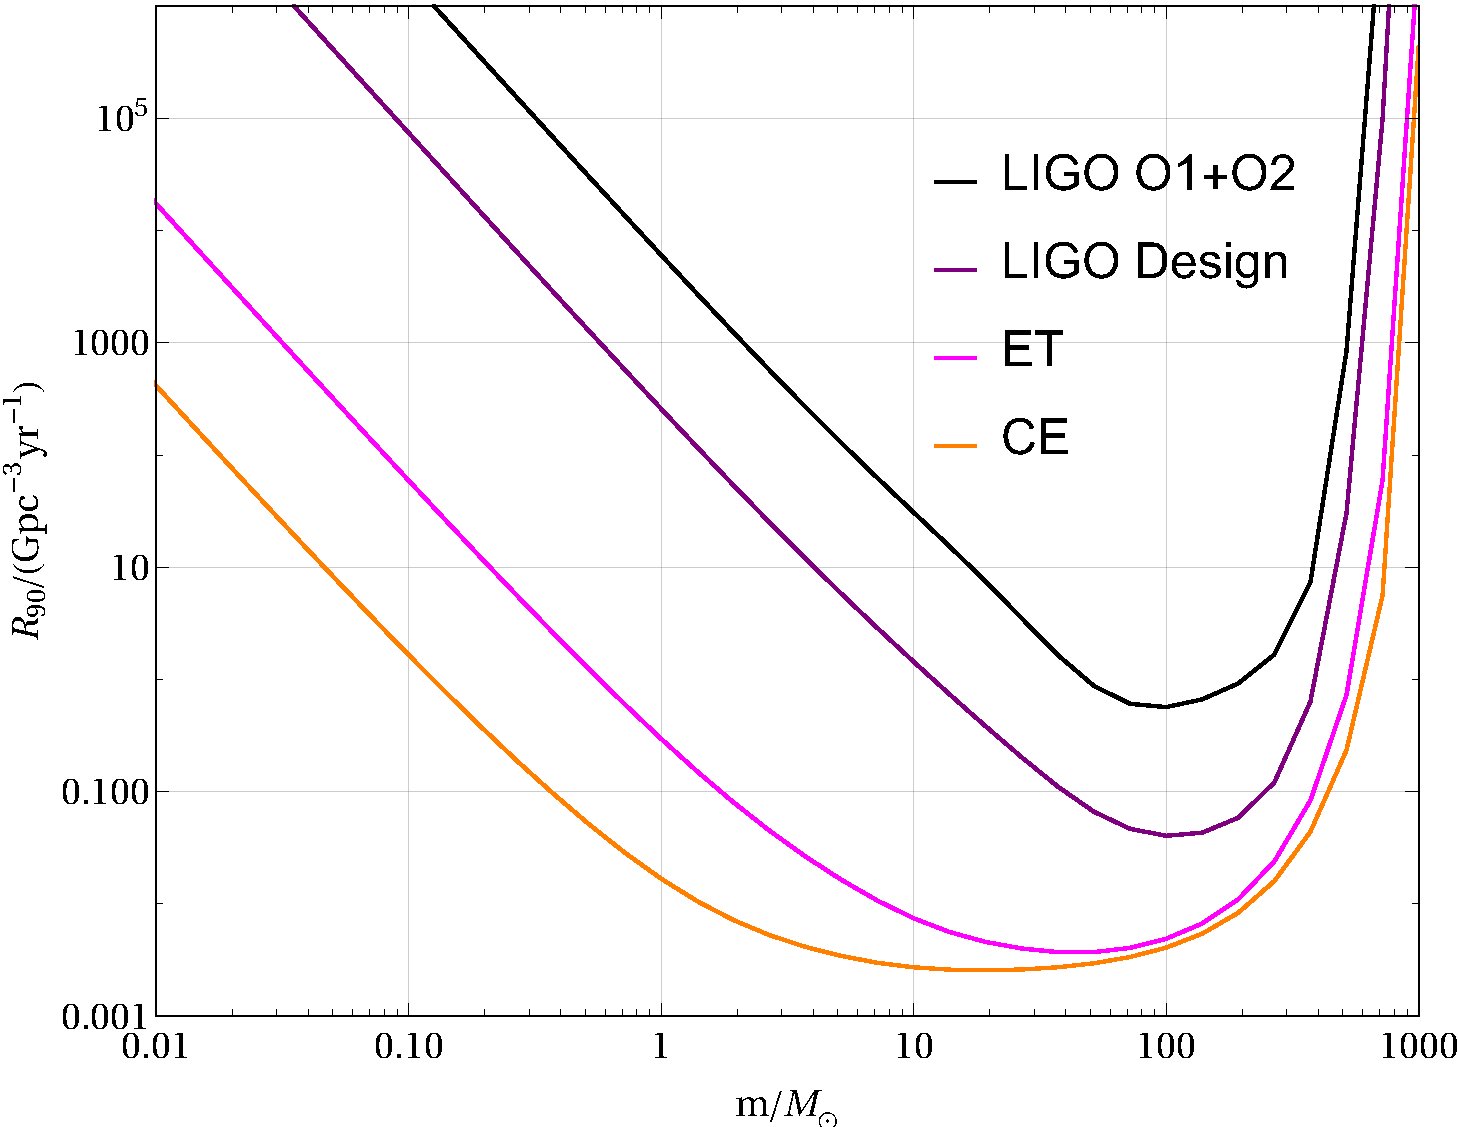
\includegraphics[width=0.9\textwidth]{R90.pdf}
    \bicaption{\label{R90_plot}LIGO O1 \& O2、LIGO设计、ET和CE给出的等质量双黑洞并合率的$90\%$上限$R_{90}$。}{The $90\%$ confidential upper limit on the binary merger rate, $R_{90}$, as a function of the masses of the equal-mass binary black holes for LIGO O1 \& O2, LIGO Design, ET and CE.}
\end{figure}

通过考虑所有原初黑洞和背景的线性密度涨落所提供的角动量,单色质量谱情况下的共动局部并合率$R(z)$随红移$z$的演化由以下公式给出\cite{Ali-Haimoud:2017rtz,Chen:2018czv}
\e\label{mono_R} 
R(z) = 3.9 \times 10^6 \times \({\frac{t(z)}{t_0}}\)^{-\frac{34}{37}}
m^{-32/37} f^2 \(f^2 + \seq^2\)^{-21/74},
\q 
其中,$m \Msun$是在源参考系测量的双黑洞的质量,而$\sigma_{\mathrm{eq}}$是在辐射-物质平衡时期,其余暗物质在$\Od(10^0\sim10^3) M_\odot$尺度上的密度扰动的方差。
参照文献\cite{Ali-Haimoud:2017rtz,Chen:2018czv},我们选择$\sigma_{\mathrm{eq}}\approx 0.005$。这里$\fpbh \equiv \Omega_{\mathrm{PBH}}/\Omega_{\mathrm{CDM}}$是冷暗物质中原初黑洞所占的能量密度的百分比,与非相对论物质中原初黑洞的总丰度$f$相关,具体关系为$\fpbh \approx f/0.85$。此外,$t(z)$是在红移$z$时的宇宙时间,而$t_0\equiv t(0)$是我们宇宙的年龄。

\begin{figure}[p!]
    \centering
    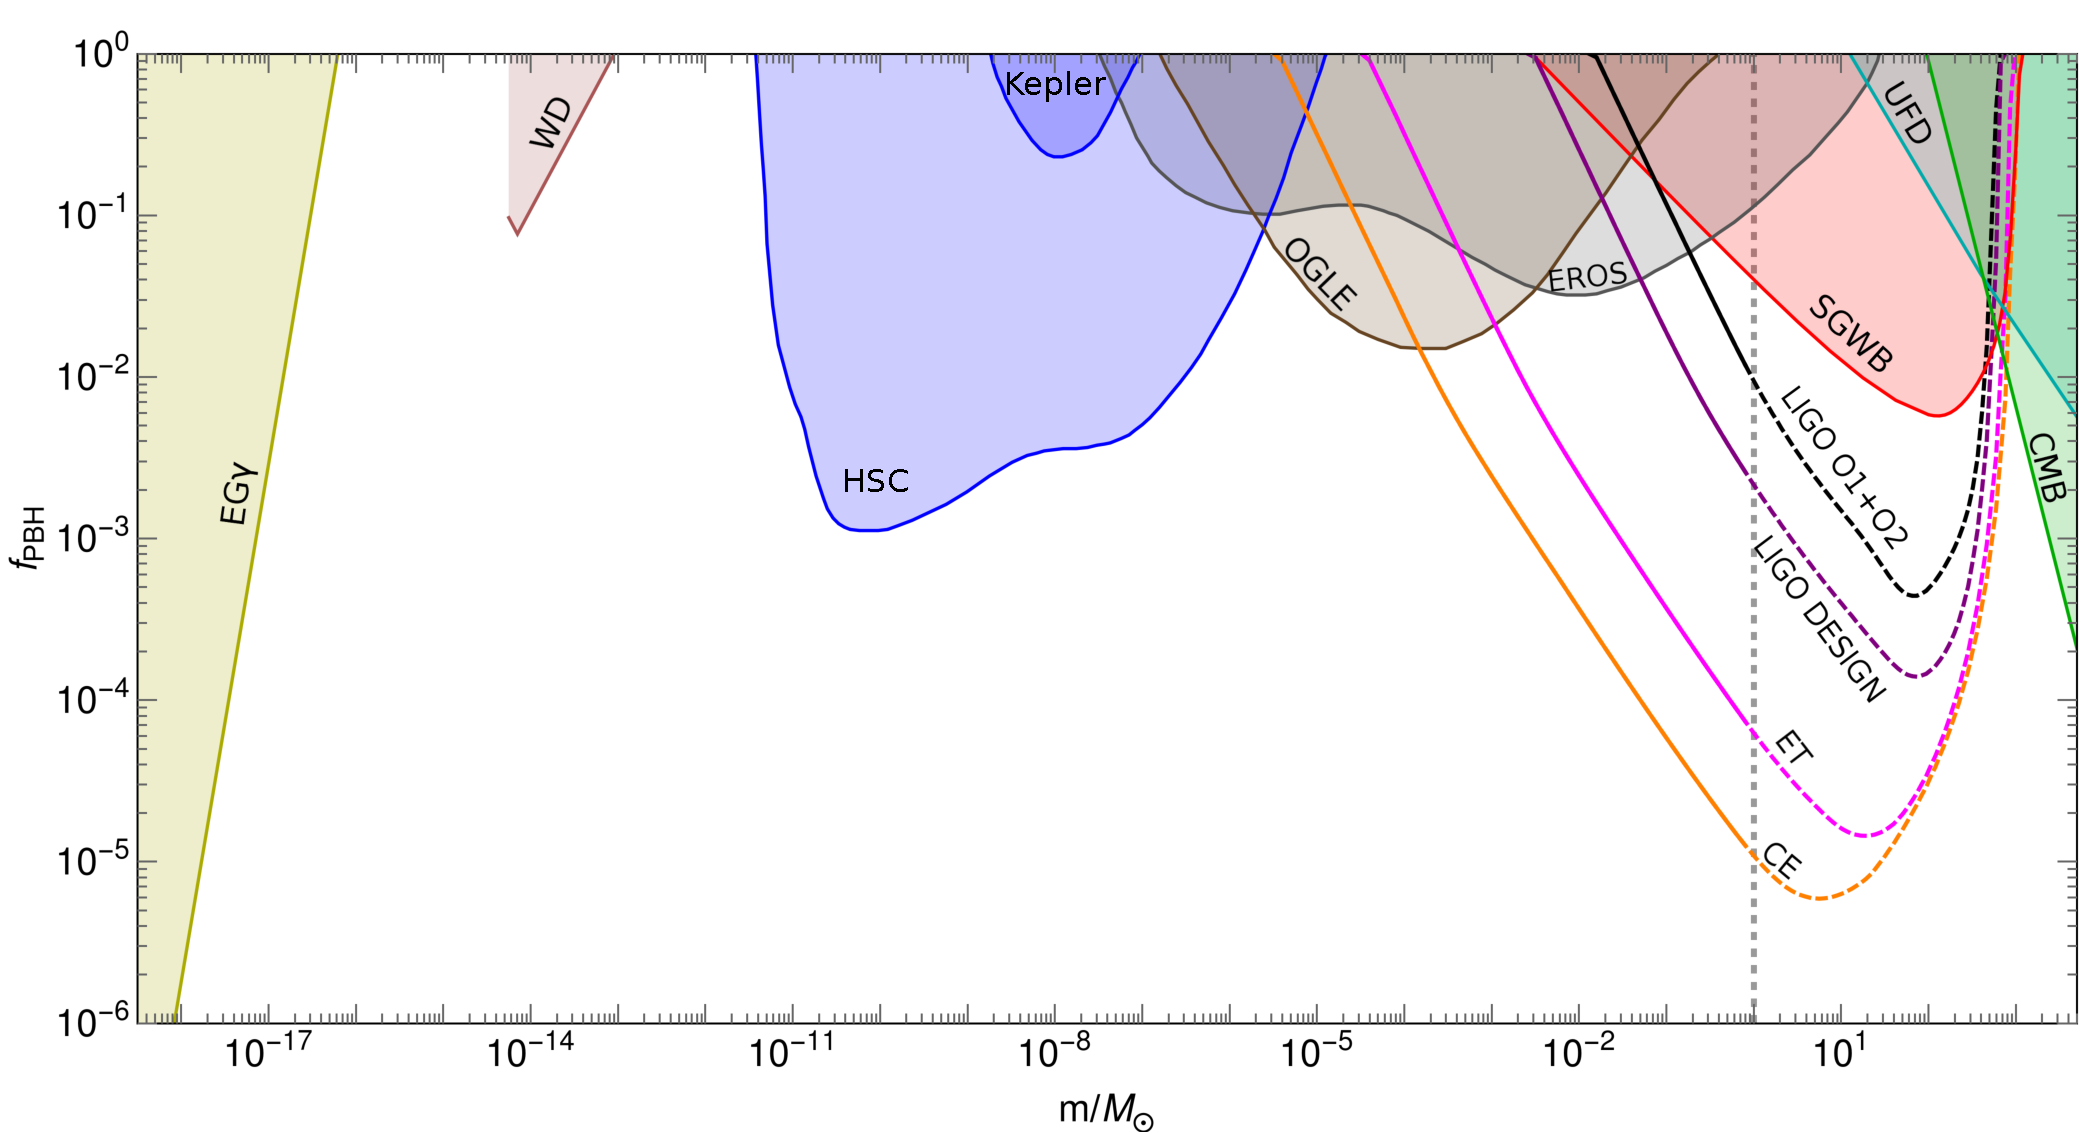
\includegraphics[width=\textwidth]{fpbh_m.pdf}
    \bicaption[由未探测到随机引力波背景和未探测到双黑洞并合对具有单质量分布的原初黑洞丰度$\fpbh$的限制。由于目前无法得知\lvc 探测到的双黑洞中到底有没有原初双黑洞,所以我们在图上$1\Msun$处用灰色竖线表示目标搜索的限制结果只对亚太阳质量的原初黑洞有效。黑色、紫色、洋红色和橙色曲线分别是LIGO O1/O2、LIGO设计、ET和CE的目标搜索给出的可探测极限。LIGO设计、ET和CE的观测时间均假设为$1$年。红色曲线代表由于LIGO O1和O2未探测到随机引力波背景给、本地星系中存在白矮星(WD) 、Subaru HSC微透镜(HSC)、开普勒毫/微透镜(Kepler)、EROS/MACHO微透镜(EROS)、OGLE微透镜(OGLE)、超暗矮星系(UFD)的动态加热以及微波背景辐射对$\fpbh$限制的结果。]{\label{fpbh1} 由未探测到随机引力波背景和未探测到双黑洞并合对具有单质量分布的原初黑洞丰度$\fpbh$的限制。由于目前无法得知\lvc 探测到的双黑洞中到底有没有原初双黑洞,所以我们在图上$1\Msun$处用灰色竖线表示目标搜索的限制结果只对亚太阳质量的原初黑洞有效。黑色、紫色、洋红色和橙色曲线分别是LIGO O1/O2、LIGO设计、ET和CE的目标搜索给出的可探测极限。LIGO设计、ET和CE的观测时间均假设为$1$年。红色曲线代表由于LIGO O1和O2未探测到随机引力波背景给出的$\fpbh$的上限。这里还给出了其他实验:星系外伽马射线(EG$\gamma$)\cite{Carr:2009jm}、本地星系中存在白矮星(WD) \cite{Graham:2015apa}、Subaru HSC微透镜(HSC)\cite{Niikura:2017zjd}、开普勒毫/微透镜(Kepler)\cite{Griest:2013esa}、EROS/MACHO微透镜(EROS) \cite{Tisserand:2006zx}、OGLE微透镜(OGLE)\cite{Niikura:2019kqi}、超暗矮星系(UFD)的动态加热\cite{Brandt:2016aco}以及微波背景辐射\cite{Ali-Haimoud:2016mbv,Blum:2016cjs,Horowitz:2016lib,Chen:2016pud,Poulin:2017bwe}对$\fpbh$限制的结果。
    }{Constraints on the abundance of primordial black holes, $\fpbh$, 
        with a monochromatic mass distribution both by the non-detection of SGWBs and the null targeted search result of binary black holes. The gray vertical line at $1\Msun$ indicates that the constraints from the targeted search are only valid for the sub-solar mass primordial black holes, because we yet cannot conclude that none of the ten binary black holes detected by \lvc\ are of primordial-origin binary black holes. The black, purple, magenta and orange curves are the results of targeted search from LIGO O1 \& O2, LIGO Design, ET and CE, respectively. The observing times of LIGO Design, ET and CE are all assumed to be $1$ year. The red curve is the updated upper bound of $\fpbh$ constrained by the non-detection of SGWB from both LIGO O1 and O2 searches. The results from other experiments are also shown here: extra-galactic gamma-ray (EG$\gamma$) \cite{Carr:2009jm}, existence of white dwarfs in our local galaxy (WD) \cite{Graham:2015apa}, Subaru HSC microlensing (HSC) \cite{Niikura:2017zjd}, Kepler milli/microlensing (Kepler) \cite{Griest:2013esa}, EROS/MACHO microlensing (EROS) \cite{Tisserand:2006zx}, OGLE microlensing (OGLE) \cite{Niikura:2019kqi}, dynamical heating of ultra-faint dwarf galaxies (UFD) \cite{Brandt:2016aco}, and accretion constraints by CMB \cite{Ali-Haimoud:2016mbv,Blum:2016cjs,Horowitz:2016lib,Chen:2016pud,Poulin:2017bwe}.}
\end{figure}

对某个引力波探测器,其预期可探测的事件数$\Nobs$为\cite{Chen:2018czv,Kavanagh:2018ggo}
\e\label{Nobs} 
\Nobs = \int R(z) \frac{\rd VT}{\rd z} \rd z,
\q 
其中$\rd VT/\rd z$是引力波探测器的可探测时空区域\cite{Abbott:2016nhf,Abbott:2016drs},表明该探测器对并合事件的选择效应。一般来说,$\rd VT/\rd z$是红移的函数,而且取决于双黑洞的属性$\xi$ (例如质量和自旋),其具体表达式为
\e 
\frac{\rd VT}{\rd z} = \frac{\rd V_c}{\rd z} \frac{\Tobs}{1+z} f(z|\xi),   
\q 
其中,$V_c$是共动体积,$\Tobs$是观测时间,分母$1+z$将宇宙时间从源参考系转换到探测器参考系。
这里$0 < f(z|\xi) < 1$是指在红移$z$时,在给定参数$\xi$下探测到双黑洞的概率\cite{OShaughnessy:2009szr}。
然后,可以通过使用最强事件统计范式(loudest event statistic formalism)来获得双黑洞并合率的$90\%$上限\cite{Biswas:2007ni}。
\e\label{R90} 
R_{90} = \frac{2.303}{VT},
\q
其中 
\e\label{VT}
VT = \int \frac{\rd VT}{\rd z} \rd z.
\q
我们采用了来自文献\cite{Abbott:2016nhf,Abbott:2016drs}的半解析近似的方法来计算$VT$。我们忽略了黑洞的自旋效应,并使用\texttt{IMRPhenomPv2}波形作为双黑洞并合的模板。此外,我们将单探测器的信噪比阈值设为$\SNR=8$作为可探测标准,这大致相当于两个探测器构成的探测网络的阀值为$12$。\Fig{R90_plot}显示了由\Eq{R90}估计出来的等质量双黑洞并合率的$90\%$上限。




\Fig{fpbh1}显示了LIGO O1/O2、LIGO设计、ET和CE通过目标搜索可得到的原初黑洞丰度$\fpbh$的可探测极限。我们假设在这些实验中没有探测到原初双黑洞。LIGO O1\& O2的总的有效观测时间为$165.6$天\cite{TheLIGOScientific:2016pea,TheLIGOScientific:2017qsa}。同时假定LIGO设计、ET和CE的运行时间都是全勤$1$年。文献\cite{Abbott:2018oah,Magee:2018opb}中通过对双黑洞的目标搜索,给出了质量范围为$\[0.2, 1\]\Msun$的亚太阳质量原初黑洞的$\fpbh$的上限。我们从几个方面来推广了文献\cite{Abbott:2018oah,Magee:2018opb}的结果。首先,我们采用了在文献\cite{Ali-Haimoud:2017rtz}中提出的并合率,与 文献\cite{Abbott:2018oah,Magee:2018opb}使用的来自文献\cite{Sasaki:2016jop}给出的并合率相比,我们所使用的并合率更全面地考虑了双黑洞系统的演化。其次,我们还通过提出用第三代引力波探测器(如CE和ET)来估计了$\fpbh$的可探测极限。最后,我们并不局限于$\[0.2, 1\]\Msun$的质量范围,而是扩展到探测器的可探测质量范围。在解释\Fig{fpbh1}的结果时应该小心。由于目前观测到的超太阳质量双黑洞是否属于原初双黑洞还有争议,我们用虚线来表明超太阳质量原初黑洞的可探测极限。
此外,当质量小于$0.2\Msun$,从引力波数据中搜索信号的难度会大幅增加。这是因为对于小质量系统,模板的起始频率也小;而做模板匹配所需的模板数量$\Ntemp$正比于最小质量$\Mmin$和起始频率$\fmin$\cite{Magee:2018opb}
\e 
\Ntemp \propto \(\Mmin  \fmin\)^{-8/3}.
\q
计算资源的急剧增加限制了目前的引力波探测能力,使其无法有效地处理质量远低于$0.2\Msun$的双黑洞系统。然而,在未来,这个问题可能会通过改进搜索算法或计算技术来解决。我们给出CE和ET的结果的主要目的是为了说明未来探测器的探测能力。还需要注意的是,文献\cite{Ali-Haimoud:2017rtz,Kavanagh:2018ggo}通过使用\lvc\ O1数据中给出了质量范围为$[10, 300]\Msun$的原初黑洞的丰度$\fpbh$的上限。我们通过使用\lvc\ O1和O2数据更新了文献\cite{Ali-Haimoud:2017rtz,Kavanagh:2018ggo}的限制结果。所以我们得到的上限比文献\cite{Ali-Haimoud:2017rtz,Kavanagh:2018ggo}的结果更加严格。

由于\lvc 没有探测到随机引力波背景,文献\cite{Wang:2016ana}给出了$\fpbh$的上限。我们更新了\cite{Wang:2016ana}的结果,给出了$\fpbh$更严格的限制。通常人们可能会以为由目标搜索给出的原初黑洞丰度的限制要比由随机引力波背景给出的限制更严格。虽然来自轻质量的双黑洞并合产生的引力波信号非常微弱,无法被引力波探测器直接探测到,但是这些微弱的信号可以叠加形成一个可探测的随机引力波背景。所以未探测到随机引力波背景会对轻质量的原初黑洞的丰度给出更严格的限制。请看\Fig{fpbh1}中$0.1 \Msun$附近红曲线和黑曲线的交叉。其实,对于其他的探测实验(比如LIGO设计、ET和CE)也有类似的结果。

%%%%%%%%%%%%%%%%%%%%%%%%%%%%%%%%%%%%%%%%%%%%%%%%%%%%%%%%%%%%%%%%%%%%%%%%%%%%%%%%
\subsection{\label{general}原初黑洞具有一般质量谱的情况}

\lvc 在其O1和O2观测阶段的数据中搜索了两个黑洞都具有亚太阳质量的双黑洞系统,发现数据中并没有该类信号\cite{Abbott:2018oah,Magee:2018opb,Authors:2019qbw},并给亚太阳质量的原初黑洞的丰度给出了限制。然而,该搜索只考虑成分质量在$0.2\Msun$到$1\Msun$之间的原初双黑洞系统。在这一小节中,我们提出搜索两个质量分别是亚太阳质量和超太阳质量的黑洞构成的原初双黑洞系统。由于这样的系统可以发出更强的引力波,从而更容易被探测到。

在这里,我们将前一小节的讨论扩展到原初黑洞具有一般质量分布的情况。我们假设迄今为止由\lvc 观察到的所有双黑洞都是原初双黑洞。之前的工作\cite{Chen:2018rzo,Raidal:2017mfl,Kocsis:2017yty,Raidal:2018bbj} 通常选择一些特定的质量函数,例如幂律质量谱或对数正态质量谱,来描述原初黑洞质量分布。这些特定的质量谱通常来自特定的原初黑洞形成模型。在这里,我们采取一种与模型无关的方法,即将质量函数$P(m)$从$0.2 \Msun$到$100 \Msun$进行分段
\e\label{para} 
P(m) = \begin{cases} 
    P_0, & 0.2\, \Msun \leq m < 1\, \Msun \\
    P_1, & 1\, \Msun \leq m < 30\, \Msun \\
    P_2, & 30\, \Msun \leq m < 60\, \Msun \\
    P_3, & 60\, \Msun \leq m \leq 100\, \Msun
\end{cases}
\q 
其中$P_i = \{ P_0, P_1, P_2, P_3 \} $为四个常数,其满足归一化条件
\e 
\int P(m)\, \rd m = 0.8P_0 + 29P_1 + 30P_2 + 40P_3 = 1.
\q 
这里,四个$P_i$中只有三个是独立的,我们选择$\vth = \{P_1, P_2, P_3\}$作为自由参数。我们将用LIGO O1和O2探测到的10个双黑洞去拟合$\vth$。在本小节中,我们感兴趣的原初黑洞的质量范围为$\[\mmin, \mmax\] = \[0.2\Msun, 100\Msun\]$。这里$\mmin=0.2\Msun$对应于LIGO搜索亚太阳质量超轻双黑洞的质量下限\cite{Abbott:2018oah}。

在文献\cite{Chen:2018czv}中,我们给出了具有一般质量函数的原初双黑洞的并合率分布。对于一个归一化的质量谱,时间依赖的共动并合率密度$P(m|\vth)$为
\m\label{calR} 
\mR_{12}(t|\vth) &\app& 3.9 \cdot 10^6 \times \({\frac{t}{t_0}}\)^{-\frac{34}{37}} f^2 (f^2+\sigma_{\mathrm{eq}}^2)^{-{21\over 74}} \times (m_1 m_2)^{{3\over 37}} (m_1+m_2)^{36\over 37} \nonumber \\
&& \times  \min\(\frac{P(m_1|\vth)}{m_1}, \frac{P(m_2|\vth)}{m_2}\) \({P(m_1|\vth)\over m_1}+{P(m_2|\vth)\over m_2}\),
\n
其中双黑洞的分量质量$m_1$和$m_2$的单位为$\Msun$。通过对分量质量的积分,可以得到与时间(或红移)依赖的并合率为
\e\label{Rcal2}
\mR(t|\vth) = \int \mR_{12}(t|\vth)\ \rd m_1\, \rd m_2.
\q 
进而局域并合率密度为\cite{Chen:2018rzo}
\e 
\mR_{12}(t_0|\vth) = R\, p(m_1,m_2|\vth).
\q 
我们选取局域并合率$R \equiv \mR(t_0|\vth)$使得双黑洞并合的概率密度$p(m_1,m_2|\vth)$是归一的。

\begin{figure*}[htbp!]
	\centering
	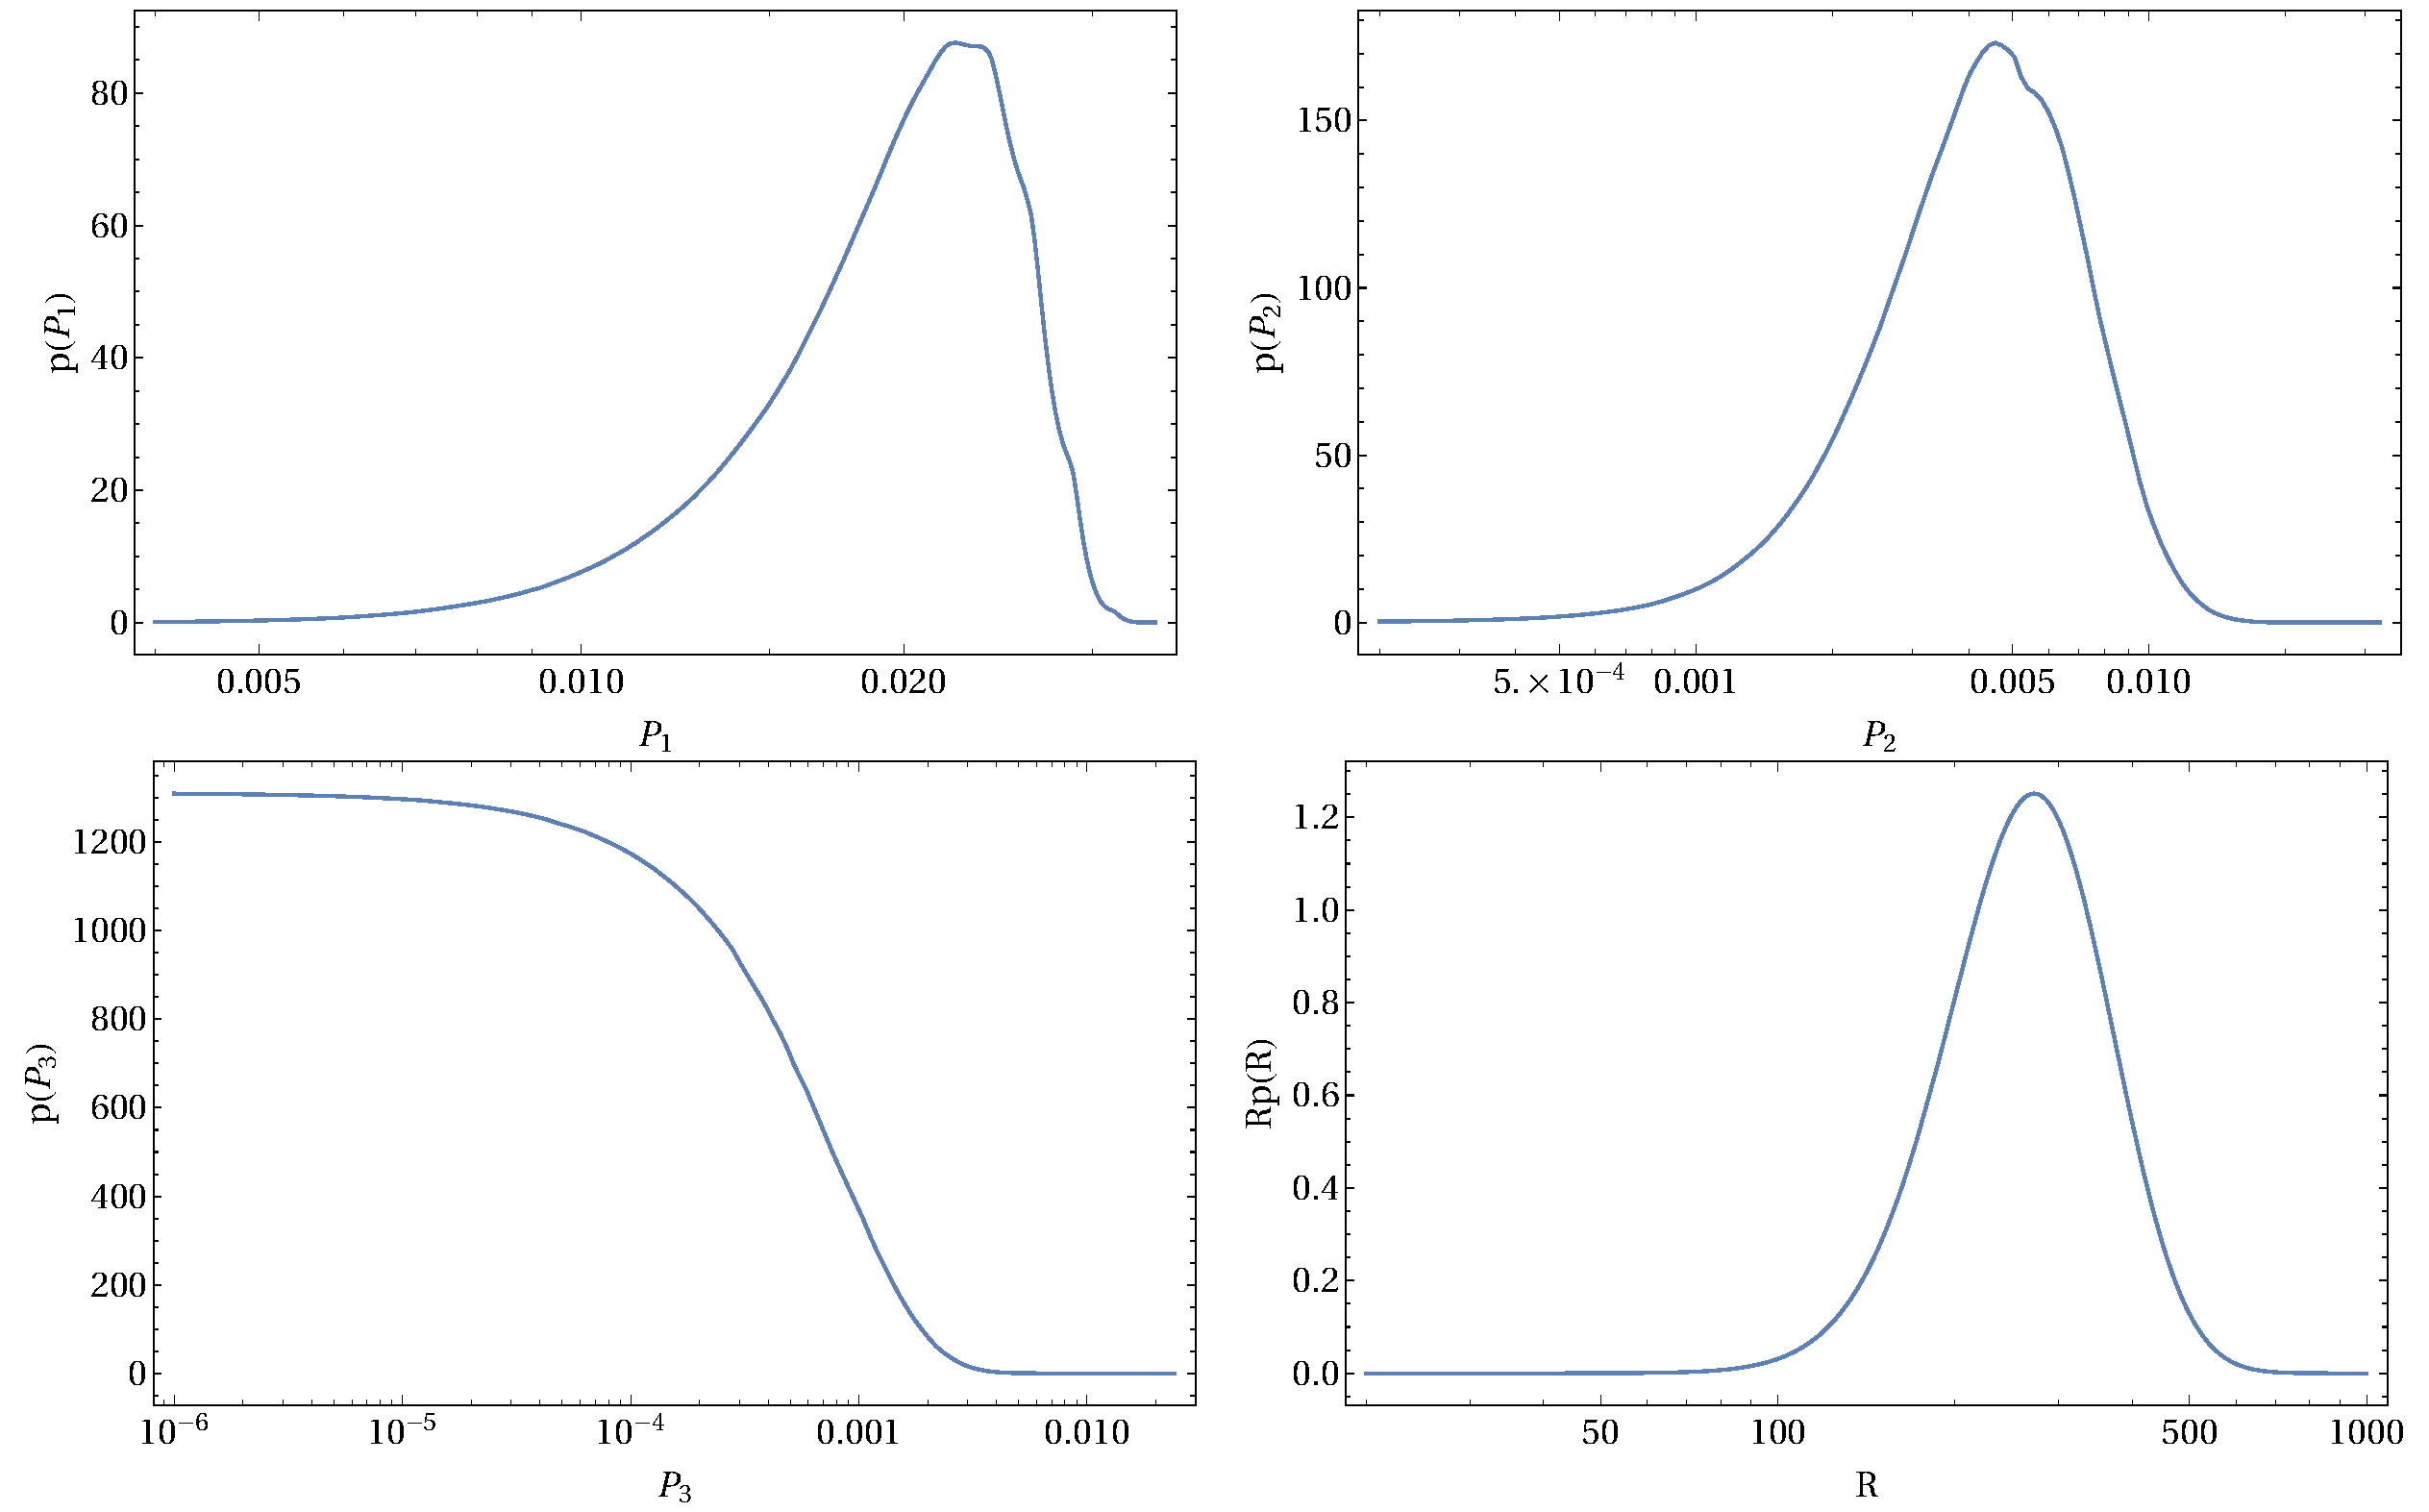
\includegraphics[width = \textwidth]{posts.pdf}
	\caption{\label{posts}
	$\{R, P_1, P_2, P_3\}$参数的后验分布。
	}{The posterior distributions for the free parameters $\{R, P_1, P_2, P_3\}$.}
\end{figure*}
为了从\lvc 观察到的并合事件中获取参数$\{\vth, R\}$的最佳拟合值,我们有必要从双黑洞质量分布做层次贝叶斯推断\cite{Abbott:2016nhf,Abbott:2016drs,TheLIGOScientific:2016pea,Wysocki:2018mpo,Fishbach:2018edt,Mandel:2018mve,Thrane:2018qnx}。
如果有$N$个双黑洞并合的数据,$\vd = (d_1, \dots, d_N)$,那么似然函数为\cite{Wysocki:2018mpo,Fishbach:2018edt,Mandel:2018mve,Thrane:2018qnx}
\e\label{likelihood}
p(\vd|\vth, R) \propto R^{N} e^{-R\, \beta(\vth)} \prod_i^N 
\int \rd\vla\ p(d_i|\vla)\ p(\vla|\vth),
\q 
其中$\vla \equiv \{m_1, m_2\}$。
由于在\lvc 做参数估计时,对于每个事件的质量参数选取的是平的分布,所以单个事件$p(d_i|\vla)$的似然函数与该事件的后验$p(\vla|d_i)$成正比。我们将使用\lvc 公开的10个双黑洞的后验分布\cite{TheLIGOScientific:2016pea,LIGOScientific:2018mvr}来估算\Eq{likelihood}的积分。同时,$\beta(\vth)$被定义为
\e 
\beta(\vth) \equiv \int \rd\vla\ VT(\vla)\ p(\vla|\vth),
\q 
其中$VT(\vla)$由\Eq{VT}给出。进而,我们可以直接估算后验概率分布$p(\vth, R|\vd)$为
\e\label{post} 
p(\vth, R|\vd) \propto p(\vd |\vth, R)\ p(\vth, R).
\q 
仿照\lvc \citep{Abbott:2016nhf,Abbott:2017vtc},我们选取$\vth$为平的分布,而$R$为对数平的分布,即
\e 
p(\vth, R) \propto \frac{1}{R}.
\q 
对\Eq{post}的 $R$进行积分,我们很容易得到边际化的后验分布 
\e\label{post_vth} 
p(\vth|\vd) \propto \[\beta(\vth)\]^{-N} 
\prod_i^N \int \rd\vla\ p(d_i|\vla)\ p(\vla|\vth).
\q
以上的后验分布已经被广泛运用于引力波参数推断中 \citep{Abbott:2016nhf,Abbott:2017vtc,TheLIGOScientific:2016pea,Abbott:2016drs,Fishbach:2017zga,Chen:2018rzo}。

\begin{figure}[h!]
    \centering
    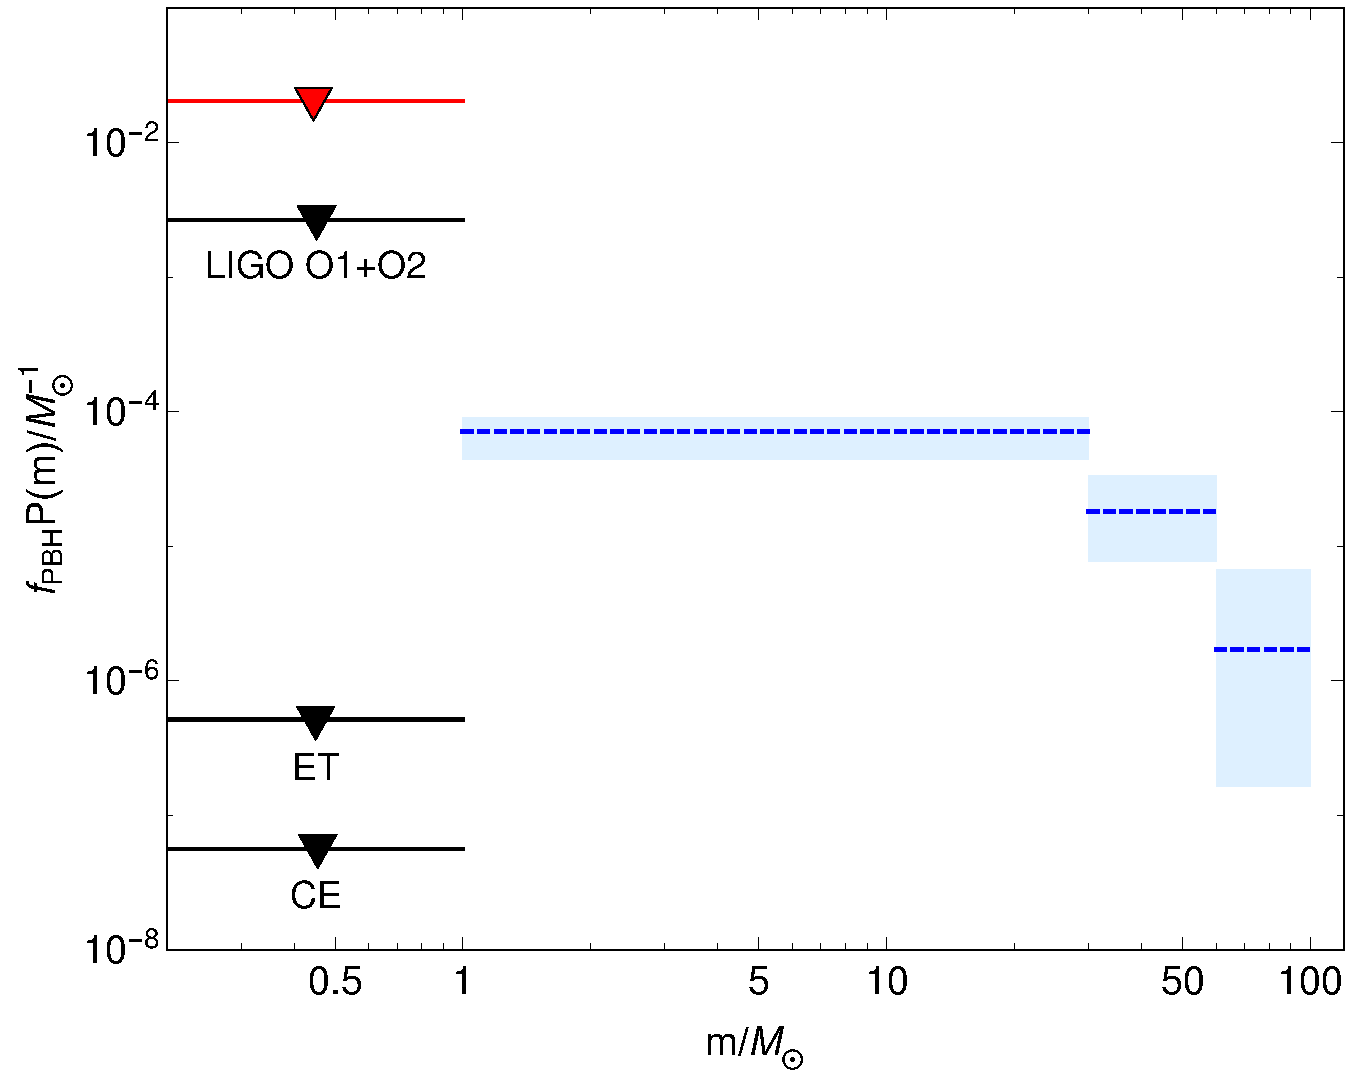
\includegraphics[width=\textwidth]{fpbhPmdm.pdf}
    \bicaption{\label{fpbhPmdm}
        对原初黑洞占冷暗物质丰度$\fpbh$的限制。蓝色区域是根据LIGO的O1和O2事件推断出来的对质量范围$1 \Msun \le m \le 100 \Msun$的限制。其中,中心虚线为中值,而阴影条代表$90\%$的泊松误差。在质量范围$[0.2, 1]\Msun$中显示的四条线分别代表了LIGO O1、LIGO O1 \& O2、ET和CE给出的限制。
    }{Constraints on the abundance of primordial black holes, $\fpbh$, in CDM.
    The blue regions with $1 \Msun \le m \le 100 \Msun$ 
    are inferred from LIGO's O1 and O2 events, 
    where the centered dashed lines are the median values and
    the shaded bars represent the $90\%$ Poisson errors.
    Four lines shown in the mass range $[0.2, 1]\Msun$ represent
    the constraints from null targeted searches of LIGO O1, 
    LIGO O1 \& O2, ET and CE, respectively.}
\end{figure}
\Fig{posts}给出了自由参数${R, P_1, P_2, P_3}$的后验分布。利用LIGO O1和O2探测到的10个双黑洞事件,我们得到参数$\{\vth, R\}$的中值和$90\%$的置信区间为
$P_1 = 2.1^{+0.7}_{-0.8} \times 10^{-2}$,
$P_2 = 5.4^{+4.7}_{-3.1} \times 10^{-3}$,
$P_3 = 5.1^{+15.2}_{-4.6} \times 10^{-4}$,
以及 $R = 308^{+193}_{-135}\, \gpcyr$。由此我们可以推断出原初黑洞占冷暗物质的丰度为$\fpbh = 3.3\,^{+2.3}_{-1.8} \times 10^{-3}$。
我们得到的原初黑洞的丰度与之前的估计是一致的,即$10^{-3} \lesssim \fpbh \lesssim 10^{-2}$。我们的结果证实了冷暗物质的主导部分不应该来源于质量范围为$[0.2, 100]\Msun$的原初黑洞\citep{Sasaki:2016jop,Ali-Haimoud:2017rtz,Raidal:2017mfl,Kocsis:2017yty,Chen:2018czv,Chen:2018rzo}。接下来我们将研究探测亚太阳质量双黑洞的可能性。
我们将质量范围为$[0.2, 1]\Msun$的原初黑洞的丰度记为 
\e 
\fpbhn \equiv \fpbh P_0 \,\Delta m_0,
\q
其中$\Delta m_0 = (1 - 0.2) \Msun = 0.8 \Msun$。
从上述得到的结果,我们可以通过LIGO的O1和O2数据直接推断出$\fpbhn$的上限为$\fpbhn \le 1.8 \times 10^{-3}$。未来,如果第三代地基引力波探测器投入运行,探测能力将大大增强。如果真的存在亚太阳质量双黑洞,我们将有更多机会探测到它们。除了寻找有两个亚太阳质量分量的双黑洞外,我们还建议寻找由一个亚太阳质量分量黑洞(质量在$[0.2, 1]\Msun$)和一个超太阳质量黑洞(质量在$[1, 100]\Msun$)构成的双黑洞系统。利用最强事件统计范式[见\Eq{R90}]和从LIGO的O1和O2数据推断出的$\vth$的值,$\fpbhn$可以被限制在一个前所未有的水平。假设没有双黑洞被探测到,ET可以得到$\fpbhn$的可探测极限为$\fpbhn \le 4.1 \times 10^{-7}$,而CE可以得到$\fpbhn$的可探测极限为 $\fpbhn \le 4.5 \times 10^{-8}$。\Fig{fpbhPmdm}显示了当原初黑洞具有一般的质量分布时,对$\fpbh$和$\fpbhn$的可探测限制。假设原初黑洞的质量在$[0.2, 1]\Msun$是平的分布,\Fig{fpbhPmdm}中的红线显示了未搜到亚太阳质量双黑洞而给出的$\fpbh$的上限。可以看出,搜索由亚太阳质量黑洞和超太阳质量黑洞构成的双黑洞得到的$\fpbh$的可探测极限,比搜索两个亚太阳质量的黑洞构成的双黑洞得到的$\fpbh$相比,将使$\fpbh$的可探测极限提高$\Od(10^2 \sim 10^3)$的数量级。


%%%%%%%%%%%%%%%%%%%%%%%%%%%%%%%%%%%%%%%%%%%%%%%%%%%%%%%%%%%%%%%%%%%%%%%%%%%%%%%%
\section{\label{stellar}用超太阳质量黑洞来区分原初黑洞和天体物理黑洞}



除了通过搜索亚太阳质量双黑洞外,还有一种方法是通过探索超太阳质量双黑洞的事件率的红移演化来区分原初黑洞和天体物理黑洞。在\cite{Chen:2018czv}中,我们发现原初双黑洞的并合率随着红移$z$的增加而增加,即$\mR(z) \propto t(z)^{-34/37}$,这与原初黑洞的丰度和质量函数都无关。然而,天体物理双黑洞预测的并合率首先会随着$z$的增加而增加,然后在某个小红移处达到峰值,最后会随着$z$的增加而迅速降低。\Fig{R_z}显示了原初双黑洞和天体物理双黑洞的并合率作为红移$z$的演化函数。可见这两个模型的并合率在红移越高时差异越大。目前,LIGO只能观测到低红移的双黑洞($z <1$),但未来的引力波探测器,如CE和ET,将能够探测到更高的红移($z \ge 10$)的双黑洞并合事件。
由于事件率随红移具有不同的分布,第三代地基探测器,如CE和ET,可以很好地区分原初黑洞和天体物理黑洞模型。 

\begin{figure}[h!]
    \centering
    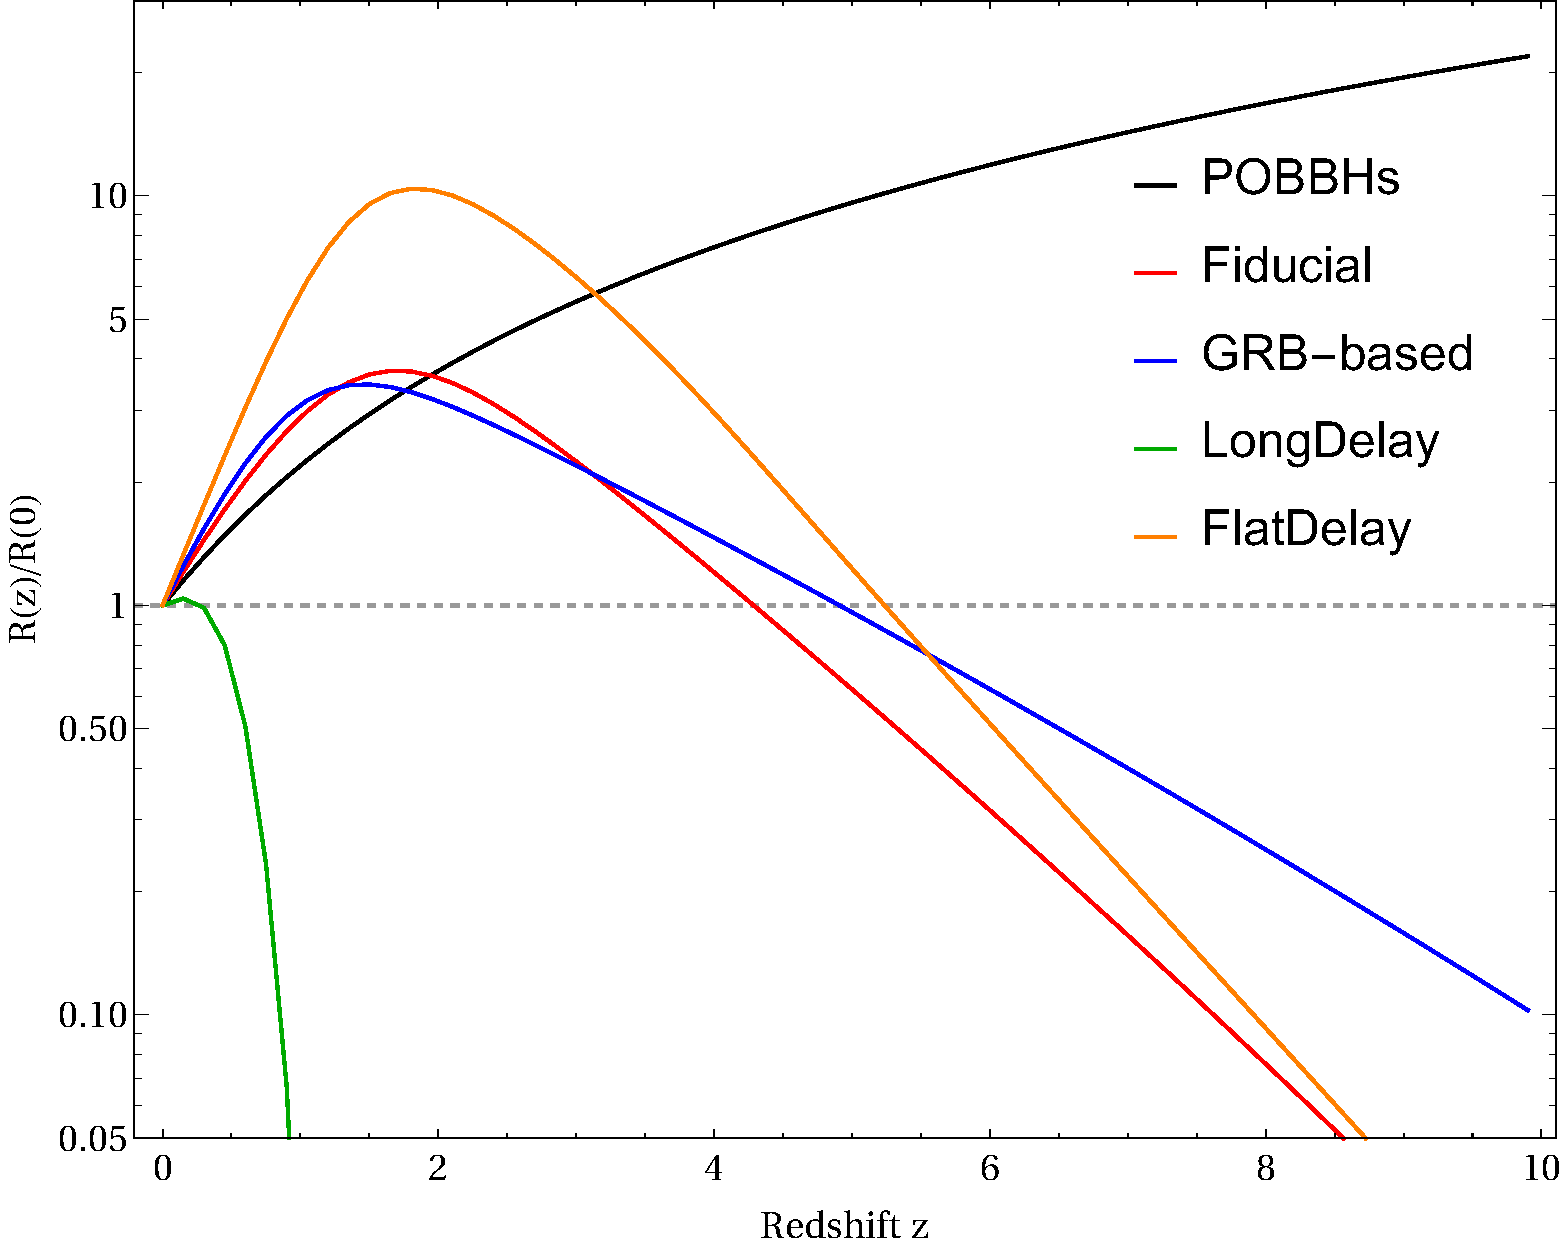
\includegraphics[width = 0.9\textwidth]{R_z.pdf}
    \bicaption{\label{R_z}
        原初双黑洞和天体物理双黑洞给出的归一化并合率的红移分布$R(z)/R(0)$。对于原初双黑洞和天体物理双黑洞,我们都只考虑双黑洞的质量范围为$5\Msun \leq m_2 \leq m_1 \leq 95 \Msun$。 我们假设原初黑洞具有一般的质量分布(见\Eq{para}),且用最佳拟合值来计算原初双黑洞的并合率。
    }{Redshift distribution of the normalized merger rate, $R(z)/R(0)$,
    for the primordial-origin binary black holes (POBBHs) and stellar-origin binary black holes, respectively.
    For both the primordial-origin binary black holes and stellar-origin binary black holes, we only count the binary black holes with masses 
    in the range of $5\Msun \leq m_2 \leq m_1 \leq 95 \Msun$.
    We assume primordial black holes have a broad mass distribution of Eq.~\eqref{para}, and the best-fits values are used to calculate the merger rate of primordial-origin binary black holes.}
\end{figure}

为了和之前的研究\citep{Abbott:2017vtc,Abbott:2017xzg}一致,
我们将双黑洞的分量质量限制在以下范围内 
$\mmin \leq m_2 \leq m_1$且$m_1 + m_2 \leq \mmax$。其中$ \mmin = 5\Msun$,$\mmax = 100\Msun$。
为了计算可观测事件率,我们首先需要知道并合率分布。
我们假设原初黑洞具有\Eq{para}的质量分布,并采用来自\ref{general}小节得到的最佳拟合值来计算并合率。而对于天体物理黑洞,并合率是天体物理黑洞的生成率$R_{\mathrm{birth}}(z,m)$与天体物理双黑洞的时间延迟分布$P_d(t_d)$的卷积\cite{Dvorkin:2016wac}
\e\label{sBHR}
\mR_{12}(z) = \int^{t_{\mathrm{max}}}_{t_{\text{min}}}  
R_{\mathrm{birth}}(t(z)-t_d, m_1) \times P_d (t_d)\ d t_d,
\q
其中$t_d$是时间延迟,$t(z)$双黑洞并合时的宇宙年龄。
生成率$R_{\mathrm{birth}}$可以通过以下方式估算出来 \citep{Dvorkin:2016wac}
\e\label{Rbirth}
R_{\mathrm{birth}}(t,m_{\mathrm{bh}})= \int \psi [t-\tau(m)]\, \phi(m)\, \delta(m- g_{\mathrm{bh}}^{-1}(m_{\mathrm{bh}}))\, dm,
\q
其中$m_{\mathrm{bh}}$是残余黑洞的质量,$\tau(m)$是质量为$m$的前身星的寿命,$\phi(m) \propto m^{-2.35}$是初始质量函数(IMF) \cite{Salpeter:1955it}。
我们考虑了``\textit{WWp}"的黑洞形成模型\citep{Woosley:1995ip},其中$m$和$m_{\mathrm{bh}}$存在以下关系
\e\label{mbhm}
\frac{m_{\mathrm{bh}}}{m}=A \left(\frac{m}{40\Msun} \right)^{\beta} \frac{1}{\left( \frac{Z(z)}{0.01 Z_\odot} \right)^{\gamma} +1},
\q 
其中$Z(z)$是金属丰度(具体形式见\cite{Belczynski:2016obo})。
\Eq{mbhm}中的参数值为:$A=0.3$,$\beta=0.8$和$\gamma=0.2$ \citep{Dvorkin:2016wac}。
解\Eq{mbhm}可以得到函数$m=g_{\mathrm{bh}}^{-1}(m_{\mathrm{bh}})$。
\Eq{Rbirth}中恒星形成率(SFR)$\psi(t)$可由以下公式计算 \citep{Nagamine:2003bd}
\e
\psi(z)= k \frac{a \exp[b(z-z_{m})]}{a-b+b \exp[a(z-z_{m})]},
\q
其中$z$是红移,$\{k, a, b, z_m\}$的参数值取决于具体的天体物理双黑洞的形成模型。在本节中,我们将考虑4个不同的天体物理双黑洞模型。

第一个为\texttt{Fiducial}模型,其中恒星形成率是对发光星系观测结果的拟合,拟合参数为$k=0.178 \, \Msun \, \mathrm{yr}^{-1}\, \mathrm{Mpc}^{-3}$, $z_{m}=2.00$, $a=2.37$, $b=1.80$ \cite{Vangioni:2014axa},时间延迟分布的形式为$P_{d} \propto t_{d}^{-1}$,并且$t_{\mathrm{min}} < t_{d} < t_{\mathrm{max}}$。其中最小延迟时间$t_{\mathrm{min}} = 50$\,Myr为双黑洞系统从形成直到并合的时间,最大延迟时间$t_{\mathrm{max}}$为哈勃时间\citep{TheLIGOScientific:2016wyq}。该模型对应于天体物理双黑洞模型的\textit{经典孤立双星演化}模型\cite{Dvorkin:2016wac}。

第二个是\texttt{GRB-based}模型,其中恒星形成率是利用高红移下的伽马射线暴(GRB)校准而得到的。这个模型中各参数取值为$k=0.146 \, \Msun \, \mathrm{yr}^{-1}\, \mathrm{Mpc}^{-3}$, $z_m=1.72$,$a=2.80$,$b=2.46$ \cite{Vangioni:2014axa}。

第三个是\texttt{LongDelay}模型,它与\texttt{Fiducial}模型基本相同,但假设最小时间延迟为$t_{\mathrm{min}}=5$Gyr,时间延迟明显变长。该模型可能与非常紧密的双星中快速旋转的大质量恒星的\textit{化学同质演化}模型相一致\cite{Mandel:2015qlu}。

最后一个是\texttt{FlatDelay} 模型,其假设时间延迟是平的分布,并且$t_{\mathrm{min}}=50$Myr和$t_{\mathrm{max}}=1$Gyr。
这个模型对应于\textit{动态形成}机制,即大多数的双星系统很可能发生在在宿主环境的极早期\cite{TheLIGOScientific:2016wyq}。

\begin{figure}[tbp!]
    \centering
    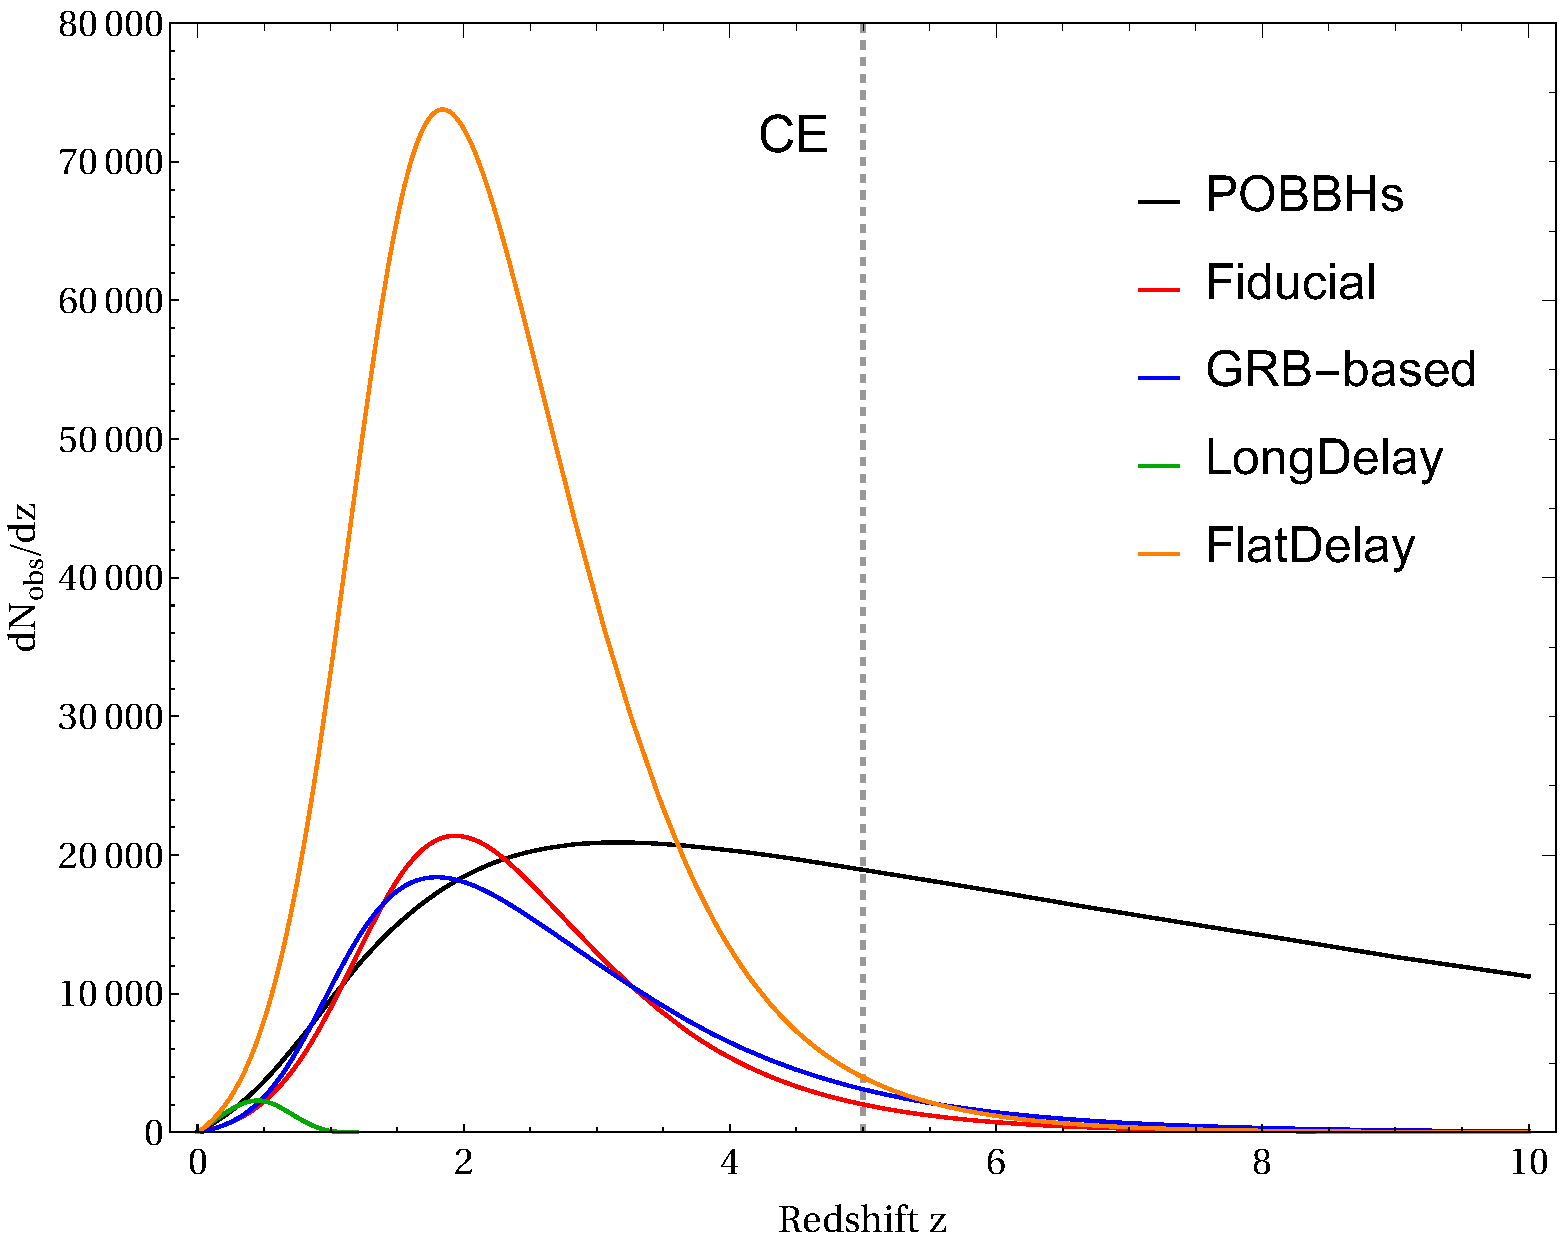
\includegraphics[width = 0.8\textwidth]{events_z_CE.pdf}\\
    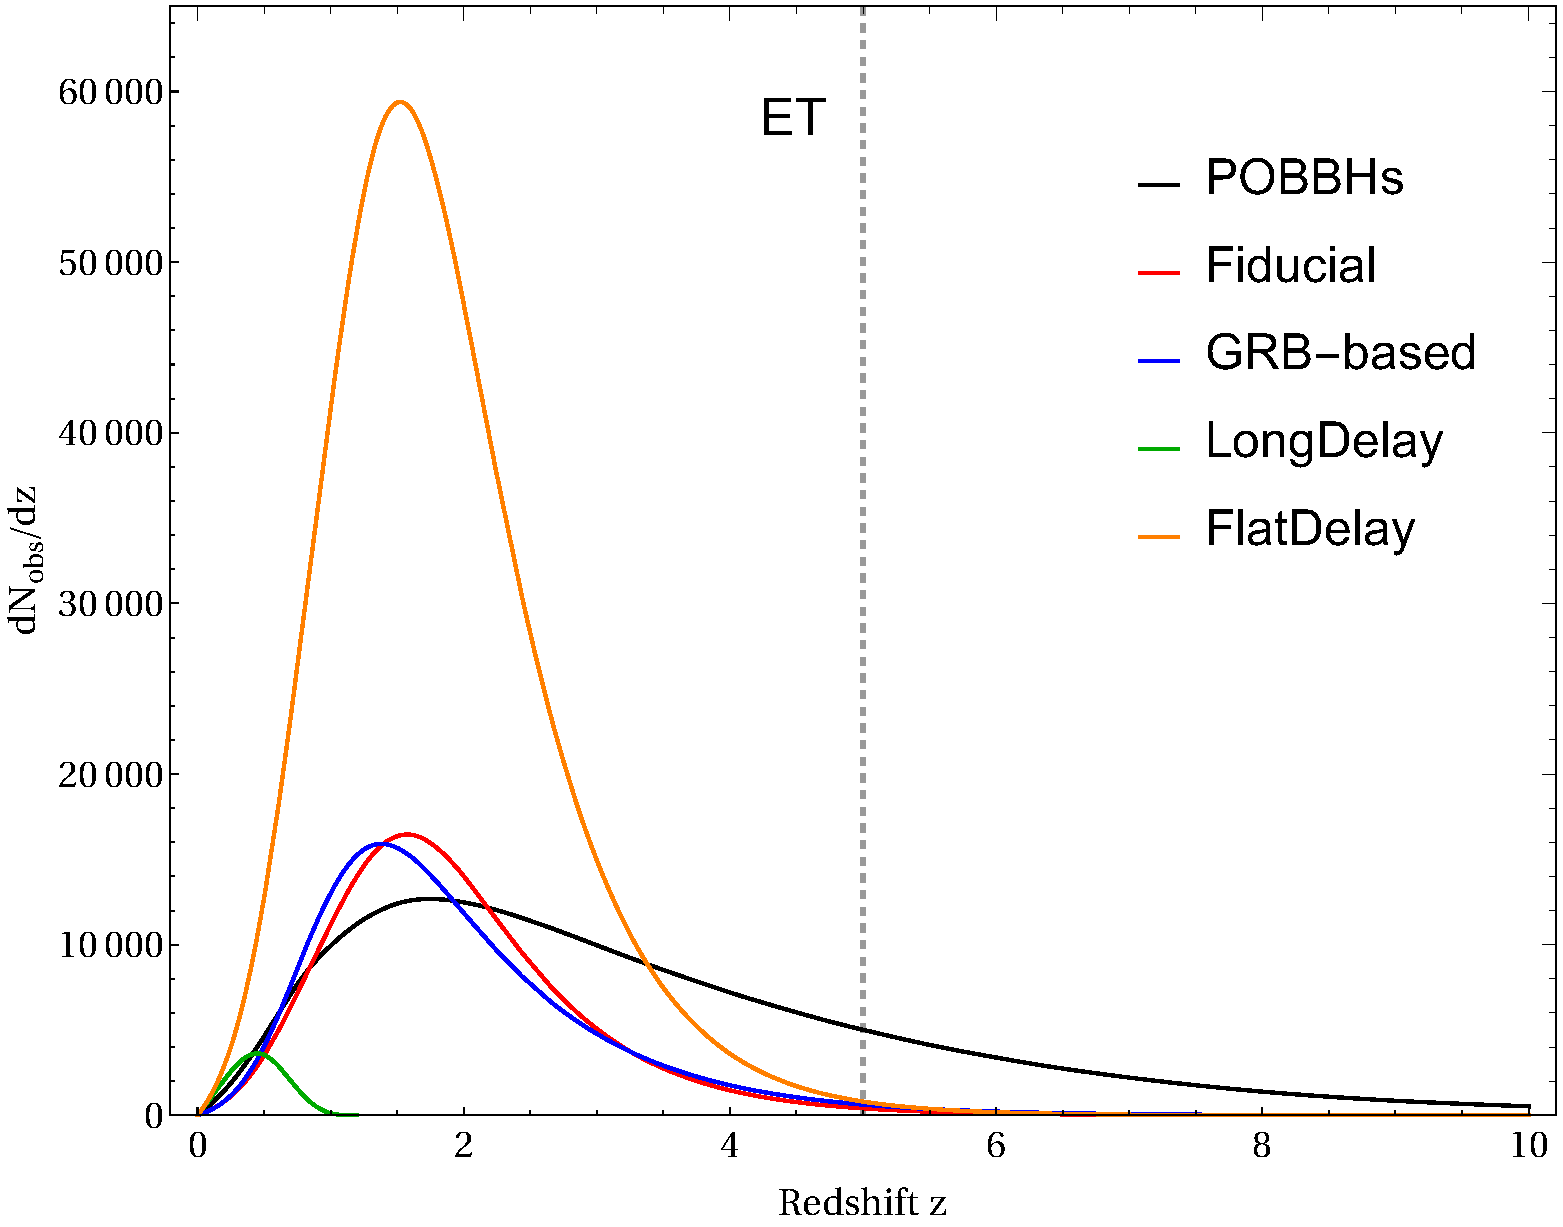
\includegraphics[width = 0.8\textwidth]{events_z_ET.pdf}
    \bicaption{\label{events_z}
        CE(上图)和ET(下图)对于双黑洞的可观测事件数密度$\rd \Nobs/\rd z$随红移的分布。对于原初双黑洞和天体物理双黑洞,我们都只考虑双黑洞的质量范围为$5\Msun \leq m_2 \leq m_1 \leq 95 \Msun$。 我们假设原初黑洞具有一般的质量分布(见\Eq{para})。
    }{Redshift distribution of the expected number density of observable binary black holes, $\rd \Nobs/\rd z$, for CE (top panel) and ET (bottom panel), respectively. For both the primordial-origin binary black holes (POBBHs) and stellar-origin binary black holes, we only count the binary black holes with masses in the range of $5\Msun \leq m_2 \leq m_1 \leq 95 \Msun$. We assume primordial black holes have a broad mass distribution of Eq.~\eqref{para}.}
\end{figure}

\begin{figure}[tbp!]
    \centering
    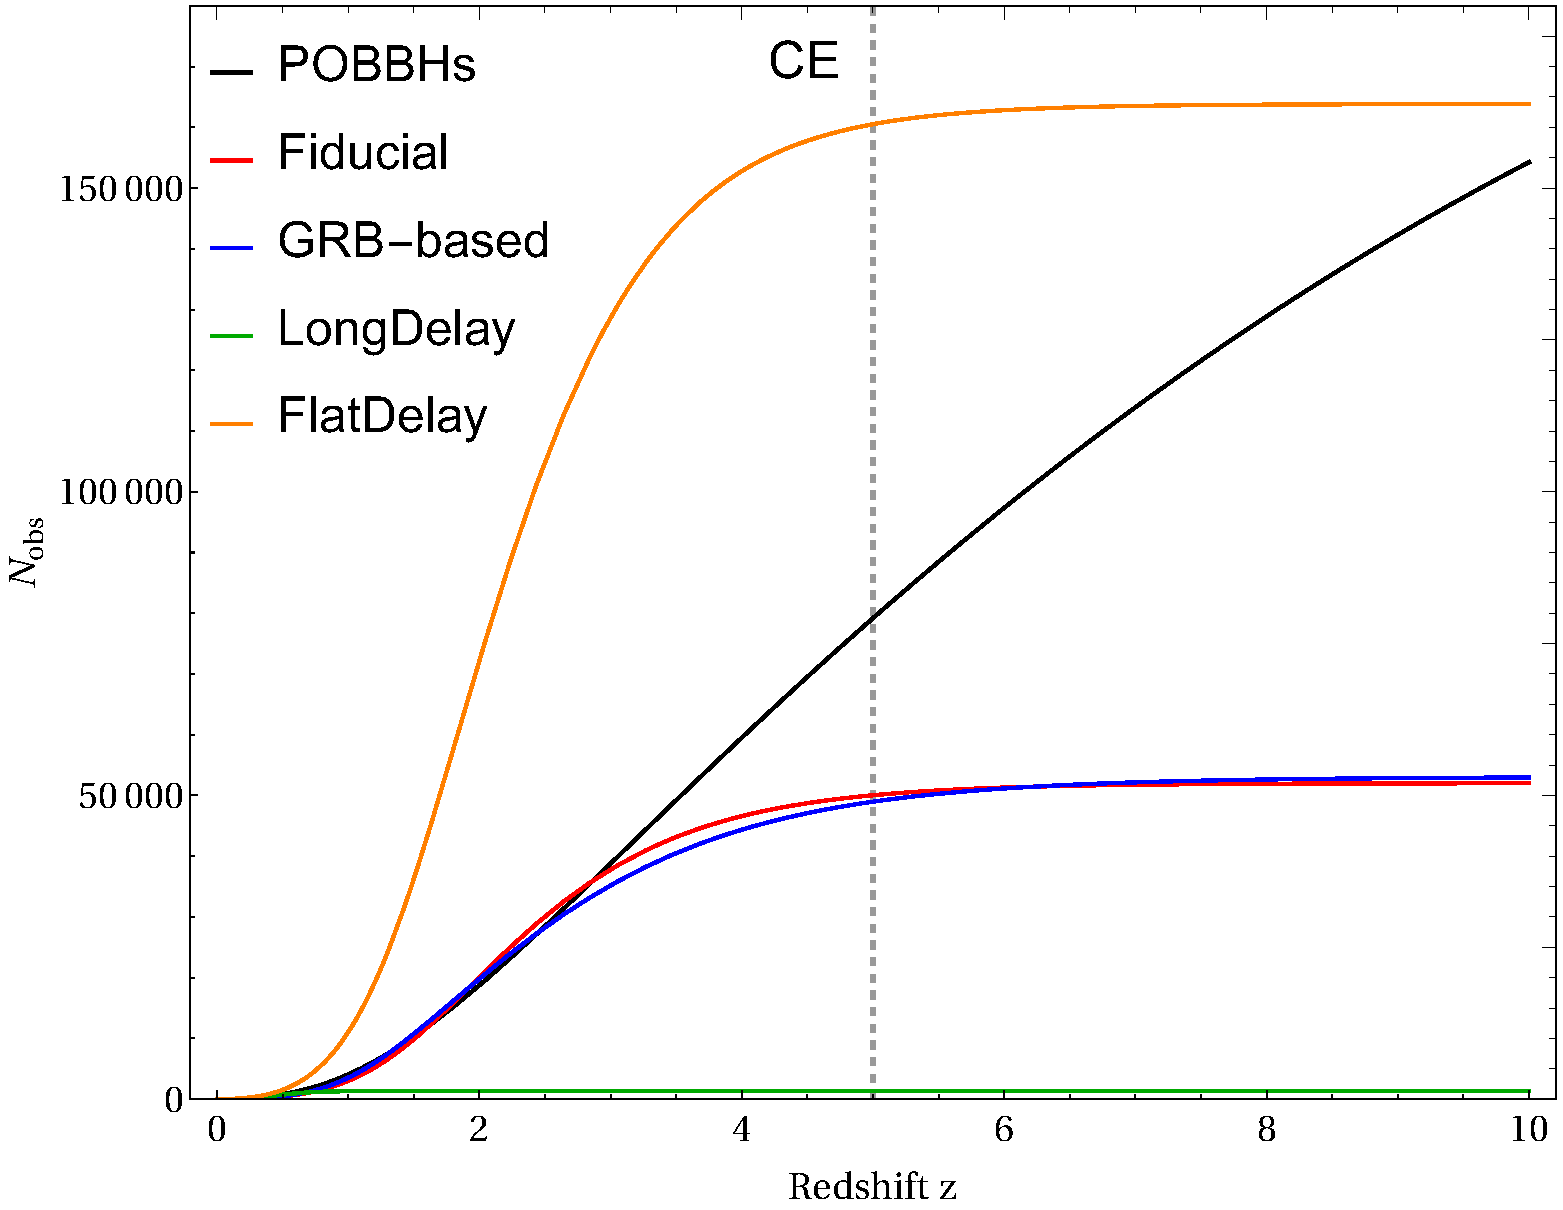
\includegraphics[width = 0.8\textwidth]{events_CE.pdf}\\
    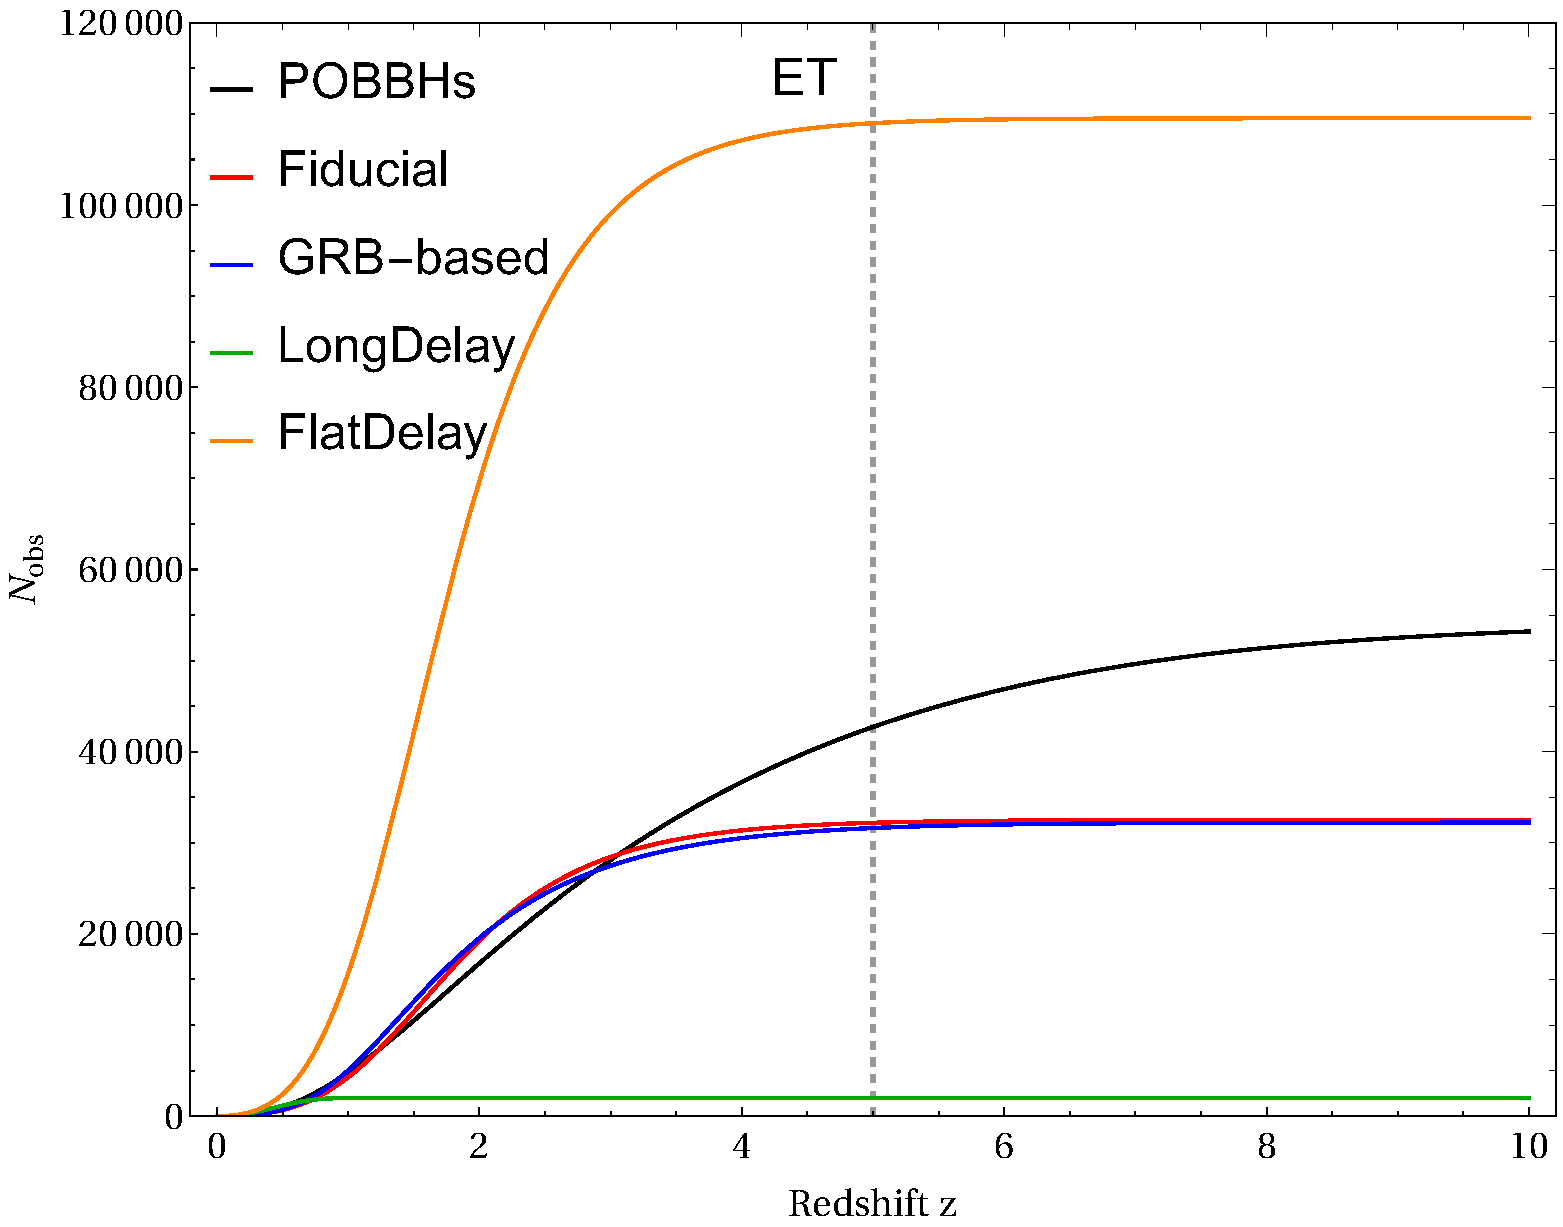
\includegraphics[width = 0.8\textwidth]{events_ET.pdf}
    \bicaption{\label{events}
        CE(上图)和ET(下图)对双黑洞的可观测总数$\Nobs$随红移的分布。对于原初双黑洞和天体物理双黑洞,我们都只考虑双黑洞的质量范围为$5\Msun \leq m_2 \leq m_1 \leq 95 \Msun$。 我们假设原初黑洞具有一般的质量分布(见\Eq{para})。
    }{Redshift distribution of the total number of observable binary black holes,
        $\Nobs$, for CE (top panel) and ET (bottom panel), respectively.
        For both the primordial-origin binary black holes (POBBHs) and stellar-origin binary black holes, we only count the binary black holes with masses 
        in the range of $5\Msun \leq m_2 \leq m_1 \leq 95 \Msun$.
        We assume primordial black holes have a broad mass distribution of Eq.~\eqref{para}.}
\end{figure}

\Fig{R_z}比较了原初双黑洞模型和不同天体物理双黑洞模型的归一化并合率$R(z)/R(0)$的红移分布。由图可知,随着红移的增加,\texttt{LongDelay}模型的并合率迅速下降;而与\texttt{Fiducial}和\texttt{FlatDelay}模型相比,\texttt{GRB-based}模型在高红移时的并合率相对较高。此外,所有天体物理双黑洞模型的并合率在高红移时都有所下降,而原初双黑洞模型的并合率在高红移时有所上升。
对于某个引力波探测器,与红移依赖的可观测事件数密度可以用以下公式计算出来
\e\label{event_density} 
\frac{\rd \Nobs}{\rd z} = \int \rd m_1 \rd m_2\, \mR_{12}(z)\,
\frac{\rd VT}{\rd z}.
\q 
对红移$z$进行积分,可得出可观测事件的总数$\Nobs$,
\e\label{Nobs2} 
\Nobs = \int \rd z \frac{\rd \Nobs}{\rd z}.
\q 
需要注意的是当$m_1 = m_2 = m$时,\Eq{Nobs}是\Eq{Nobs2}的一个特例。
\Fig{events_z}显示了CE和ET对双黑洞的可观测数密度随红移的分布$\rd \Nobs/\rd z$。
\Fig{events} 显示了CE和ET的对双黑洞的可观测总数$\Nobs$随红移的分布。
像CE和ET这样的第三代引力波探测器预计每年会探测到$\Od(10^5)$的双黑洞并合事件,并且可探测更高的红移。因为原初双黑洞和天体物理双黑洞的$\rd \Nobs/\rd z$随红移分布有很大的不同,所以可用来区分这两种双黑洞形成模型。特别是,对于我们所讨论的所有$4$种天体物理双黑洞模型来说,高红移($z>5$)对可观测数密度的贡献可以忽略不计,因此可观测事件的总数$\Nobs$在$z>5$时接近于一个常数。然而,对于原初双黑洞来说,高红移的贡献不能被忽略,因此当$z>5$时,$\Nobs$仍然会增加。



%%%%%%%%%%%%%%%%%%%%%%%%%%%%%%%%%%%%%%%%%%%%%%%%%%%%%%%%%%%%%%%%%%%%%%%%%%%%%%%%
\section{\label{discuss}总结和讨论}

\lvc 已经探测到几十个双黑洞并合产生的引力波事件,为人类探索宇宙打开了另一扇窗口。理解这些双黑洞是如何形成及演化的,是一个有待解决的科学问题。在本章中,我们探讨了通过下一代地基引力波探测器,比如ET和CE,来区分原初黑洞和天体物理黑洞的可能性。

我们首先研究了直接探测亚太阳质量双黑洞并合的可能性。如果搜索到亚太阳质量的双黑洞并合,那将是原初黑洞存在的强有力证据。对于具有单色质量谱的原初黑洞模型,我们估计和预测LIGO、ET和CE对原初黑洞占冷暗物质丰度$\fpbh$的可探测限制。只有$\fpbh$大于某个限制,才有可能被相应的探测器探测到。相应的结果见\Fig{fpbh1}。为了得到更好的限制,我们进一步考虑了去搜索由一个亚太阳质量黑洞和另一个超太阳质量黑洞构成的双黑洞系统。由于质量更大,所以这样的双黑洞比两个黑洞的质量都是亚太阳质量的双黑洞更容易被探测到。我们预测,如果ET和CE没能探测到这样的双黑洞系统,那么质量为$[0.2, 1]\Msun$的原初黑洞占冷暗物质的丰度会被限制到$\Od(10^{-7})$ and $\Od(10^{-8})$的量级。相应的结果见\Fig{fpbhPmdm}。

其次,我们探讨了利用超太阳质量双黑洞并合率的红移演化来区分原初黑洞和天体物理黑洞的可能性。我们分别估计和预测了原初黑洞和天体物理黑洞模型的预期双黑洞可探测数随红移的分布。CE和ET的结果显示在\Fig{events_z}中。当CE和ET等第三代地基引力波探测器投入运行后,预计每年将探测到$\Od(10^5)$ 双黑洞并合,并达到更深的红移($z \gtrsim 10$),可探测到的双黑洞事件的红移分布可以作为区分原初黑洞和天体物理黑洞的另一种手段。

在本章中,我们假设所有的双黑洞都来自同一个形成机制。然而,这个假设可能过于简单,因为\lvc 探测到的双黑洞可能既有原初双黑洞,又有天体物理双黑洞。在这种情况下,要准确识别每个双黑洞到底是原初双黑洞还是天体物理双黑洞是相当困难的。除了双黑洞的质量和红移分布外,其他信息(例如自旋分布),对于确定双黑洞的起源也是非常重要的信息。例如,在早期宇宙中形成的原初黑洞的自旋非常小\cite{Chiba:2017rvs,Mirbabayi:2019uph,DeLuca:2019buf} ,而某些机制形成的天体物理黑洞则倾向于有相对较大的自旋分布 \cite{Kinugawa:2016ect}。
\chapter{脉冲星计时阵列对原初黑洞丰度的限制}\label{chap:PTAfPBH}

%The detection of binary black hole coalescences by LIGO/Virgo has aroused the interest in primordial black holes (原初黑洞), because they could be both the progenitors of these black holes and a compelling candidate of dark matter (暗物质). 原初黑洞 are formed soon after the enhanced scalar perturbations re-enter horizon during radiation dominated era, which would inevitably induce  gravitational waves as well. Searching for such scalar induced gravitational waves (标量诱导引力波) provides an elegant way to probe 原初黑洞. We perform the first direct search for the signals of 标量诱导引力波 accompanying the formation of 原初黑洞 in North American Nanohertz Observatory for Gravitational waves (NANOGrav) 11-year data set. No statistically significant detection has been made, and hence we place a stringent upper limit on the abundance of 原初黑洞 at $95\%$ confidence level. In particular, less than one part in a million of the total 暗物质 mass could come from 原初黑洞 in the mass range of $[2 \times 10^{-3}, 7\times 10^{-1}] \Msun$.

\section{研究背景}
在过去的几年里,\lvc 科学组织不仅探测到来自双黑洞并合\cite{Abbott:2016blz,Abbott:2016nmj,Abbott:2017vtc,  Abbott:2017gyy,Abbott:2017oio,TheLIGOScientific:2016pea,LIGOScientific:2018mvr}产生的引力波,而且探测到了双中子星并合\cite{TheLIGOScientific:2017qsa}产生的引力波。\lvc 取得的重大科学成就使得人类进入了引力波天文学和多信使天文学的新时代。为了解释\lvc 探测到的双黑洞是如何形成和演化的,人们提出了众多模型\cite{Fishbach:2017dwv,Antonini:2016gqe,Inayoshi:2017mrs,Perna:2019axr,Rodriguez:2015oxa,Rodriguez:2016kxx,Park:2017zgj,Belczynski:2014iua,Belczynski:2016obo,Woosley:2016nnw,Rodriguez:2018rmd,Choksi:2018jnq,deMink:2010zm,deMink:2016vkw,Bird:2016dcv,Sasaki:2016jop,Clesse:2016vqa,Wang:2016ana,Ali-Haimoud:2017rtz,Chen:2018czv,Chen:2018rzo,Kavanagh:2018ggo,Raidal:2018bbj,Liu:2018ess,Chen:2019irf,Yuan:2019udt,Liu:2019rnx}。作为其中的一种模型,原初黑洞模型\cite{Bird:2016dcv,Sasaki:2016jop,Chen:2018czv}最近引起了很多关注。在宇宙早期,原初黑洞是在标量曲率扰动的波长重新进入视界的时候,由于过密区域发生引力坍缩而产生的\cite{Ivanov:1994pa,Yokoyama:1995ex,GarciaBellido:1996qt,Ivanov:1997ia,Kawasaki:2006zv}。在这种情况下,原初黑洞的质量与视界质量相当\cite{Carr:1975qj},从而导致原初黑洞的质量谱比天体物理学黑洞的质量谱宽得多。

原初黑洞模型之所以吸引人,是因为它不仅可以解释\lvc 探测到的双黑洞并合事件的事件率,而且也是暗物质的候选者之一。暗物质问题仍然是困扰人类的一个未解之谜。
原初黑洞能否构成所有的暗物质还没有定论。然而原初黑洞占冷暗物质的丰度$\fpbh$
已经受到各种实验观测,例如原初黑洞产生的银河系外$\gamma$射线 \cite{Carr:2009jm}、$\gamma$射线暴的femtolensing\cite{Barnacka:2012bm}、Subaru/HSC微透镜\cite{Niikura:2017zjd}、开普勒毫/微透镜\cite{Griest:2013esa}、OGLE微透镜\cite{Niikura:2019kqi}、EROS/MACHO微透镜\cite{Tisserand:2006zx}、
本星系中的白矮星\cite{Graham:2015apa}、超暗矮星系的动态加热\cite{Brandt:2016aco}、
原初黑洞吸积星际气体产生的X射线/无线电辐射\cite{Gaggero:2016dpq}、原初黑洞吸积原初气体产生的宇宙微波背景辐射\cite{Ali-Haimoud:2016mbv,Blum:2016cjs,Horowitz:2016lib,Chen:2016pud}、亚太阳质量双黑洞并合产生的引力波\cite{Abbott:2018oah,Magee:2018opb,Chen:2019irf,Authors:2019qbw}和双黑洞并合产生的随机引力波背景\cite{Wang:2016ana,Chen:2019irf}。但是在$[10^{-16},10^{-14}] \cup [10^{-13},10^{-12}] M_\odot$的质量窗口内,原初黑洞仍然可能构成所有的暗物质。请参考文献\cite{Chen:2019irf}里关于原初黑洞实验限制的最新总结。

我们知道,在原初黑洞形成的过程中,由于曲率标量扰动将不可避免地产生标量诱导引力波。所以通过标量诱导引力波也可以探测原初黑洞暗物质。最近,研究表明标量诱导引力波背景的能量密度谱和其他引力波源的能量密度谱具有显著区别\cite{Yuan:2019wwo}。由于原初黑洞应该是由曲率扰动概率密度的尾部形成的,所以形成单个原初黑洞的概率对曲率扰动功率谱的振幅相当敏感\cite{Young:2014ana}。因此,原初黑洞的丰度对相应标量诱导引力波的振幅极为敏感。因此如果探测到标量诱导引力波将为原初黑洞的存在提供证据;而如果没有探测到标量诱导引力波将对原初黑洞的丰度产生严格的限制。


标量诱导引力波的峰值频率$(f_*)$由共动曲率扰动的功率谱的峰值决定,且与原初黑洞的质量有如下关系\cite{Saito:2008jc}
\e
f_*\sim 3\,{\rm{Hz}}\({m_{\rm{PBH}}/10^{-18} M_\odot}\)^{-1/2}.
\q
构成暗物质的原初黑洞的质量应重于$10^{-18}\Msun$,否则它们会因霍金辐射而蒸发掉。相应的标量诱导引力波的峰值频率应该低于$3$Hz,因此地基引力波探测器很难探测到相应的标量诱导引力波。另一方面,低频引力波探测器特别适合探测原初黑洞暗物质。文献\cite{Yuan:2019udt}预测了LISA\cite{Audley:2017drz}以及脉冲星计时阵列(如IPTA\cite{Hobbs:2009yy}、FAST\cite{Nan:2011um}和SKA\cite{Kramer:2015jsa})对原初黑洞丰度所能达到的观测限制。相关的工作请参见\cite{Inomata:2016rbd,Schutz:2016khr,Orlofsky:2016vbd,Dror:2019twh,Wang:2019kaf,Cai:2019elf,Clesse:2018ogk}。

尽管目前脉冲星计时阵列的数据已经被用来限制随机引力波背景的振幅,但这些结果强烈地依赖于一些特殊的幂律形式的假设,而这种幂律形式与标量诱导引力波完全不同\cite{Yuan:2019udt}。在本节中,我们将首次在公开的脉冲星计时阵列的数据集中搜索标量诱导引力波的信号,以检验原初黑洞暗物质假设。我们在NANOGrav 11年数据集中未探测到标量诱导引力波,进而给出了质量范围为$[4\times 10^{-4}, 1.7]\Msun$的原初黑洞丰度的限制。

%%%%%%%%%%%%%%%%%%%%%%%%%%%%%%%%%%%%%%%%%%%%%%%%%%%%%%%%%%%%%%%%%%%%%%%%%%%%%%%%

\section{原初黑洞的形成机制}

在这里,我们只考虑了原初黑洞具有单色质量谱的情况,其对应于$\delta$功率谱的标量曲率扰动,即
\e\label{pzeta1}
\mathcal{P}_{\zeta}(k)=A k_*\delta\(k-k_*\),
\q
其中$A$是功率谱的无量纲振幅。在这种情况下,原初黑洞的质量与峰值频率$f_*$的关系为\cite{Hawking:1971ei,Carr:1974nx}
\m\label{mkrelation}
{m_{\mathrm{PBH}}\over M_{\odot}} \simeq 2.3\times10^{18}%\left(\frac{3.91}{g_*^{\mathrm{form}}}\right)^{1 / 6}
\left(\frac{H_{0}}{f_*}\right)^{2},
\n
其中$f_*$的单位是Hz,$H_0$是哈勃常数。原初黑洞的形成是一个阈值过程,它是由高斯随机场(Gaussian random fields)的三维统计描述的,也称为峰值理论(peak theory)\cite{Bardeen:1985tr}。

在宇宙早期,由于宇宙的能量密度对原初黑洞的形成起关键作用\cite{Hawking:1971ei, Carr:1974nx},所以在形成时,原初黑洞的质量$M$和视界质量大致有如下关系
\begin{align}
    M
    &\sim
    \frac{ t }{ G }
    \sim
    10^{15}\,
    \left(
    \frac{t}{10^{-23}\,\srm}
    \right)\,
    \grm
    \, .
    \label{eq:Moft}
\end{align}
因此,原初黑洞的质量可以横跨很多个数量级。例如,在普朗克时间($10^{-43}\,\srm$)形成的原初黑洞的质量为普朗克质量($10^{-5}\,\grm$),而在$1\,\srm$形成的原初黑洞的质量可以达到$10^{5}\, M_{\odot}$。早期宇宙的高能量密度是形成原初黑洞的必要条件,但不是充分条件。如果早期宇宙存在原初不均匀性,那么高密度区域可能会停止膨胀并塌缩形成原初黑洞。在这种情况下,\Eq{eq:Moft}可以被更精确地表达为\cite{Carr:2009jm}
\begin{equation}
    M
    \approx
    2.03 \times 10^{5}\,
    \gamma
    \left( \frac{t}{1\,\srm} \right)
    M_{\odot}
    \, .
    \label{mass}
\end{equation}
其中$\gamma$是一个取决于塌缩过程的系数。在辐射为主时期,$\gamma = (1 / \sqrt{3\,})^{3} \approx 0.4$ \cite{Green:2004wb}。

我们用$\beta( M )$表示质量为$M$的原初黑洞在形成时占宇宙质量的百分数,则有\cite{Carr:2009jm}
\begin{equation}
    \beta( M )
    \equiv
    \frac{M\,n_{\mathrm{PBH}}(t_{\irm})}{\rho(t_{\irm})}
    \approx
    7.98 \times 10^{-29}\,
    \gamma^{-1/2}\,
    \left( \frac{M}{M_{\odot}} \right)^{\!3/2}\,
    \left( \frac{n_{\mathrm{PBH}}(t_{0})}{1\,\mathrm{Gpc}^{-3}} \right)
    ,
    \label{eq:beta}
\end{equation}
其中$t_{\irm}$为原初黑洞的形成时间,$n_{\mathrm{PBH}}$为原初黑洞的数密度,$g_{* \irm}$为原初黑洞形成时的相对论自由度。在今天未蒸发的原初黑洞的能量密度参数$\Omega_{\mathrm{PBH}}$大致为\cite{Carr:1975qj}
\begin{equation}
    \Omega_{\mathrm{PBH}}
    =
    \frac{M\,n_{\mathrm{PBH}}( t_{0} )}{\rho_{\mathrm{c}}}
    \approx
    \left( \frac{\beta( M )}{1.03 \times 10^{-8}} \right)
    \left( \frac{h}{0.68} \right)^{\!-2}
    \gamma^{1/2}\,
    \left( \frac{g_{* \irm}}{106.75} \right)^{\!-1/4}\,
    \left( \frac{M}{M_{\odot}} \right)^{\!-1/2}
    \,.
    \label{eq:omega}
\end{equation}
通过峰值理论可以算出原初黑洞数密度,从而求出原初黑洞在暗物质中的丰度\cite{Carr:2016drx}
\m\label{fpbh}
f_{\mathrm{PBH}}\equiv\Omega_{\mathrm{PBH}}/\Omega_{\mathrm{DM}} \simeq 1.9 \times 10^{7}
\({\zeta_c^2/A}-1\) e^{-{\zeta_c^2\over 2A}} \left(\frac{m_{\mathrm{PBH}}}{M_{\odot}}\right)^{-\frac{1}{2}},
\n
其中$\zeta_{c}\simeq1$ \cite{Musco:2008hv,Musco:2004ak,Musco:2012au,Harada:2013epa,Escriva:2019nsa,Escriva:2019phb}是形成原初黑洞的阈值。

\section{标量诱导引力波}
标量诱导引力波可以用扰动理论来计算。以往的文献只考虑标量诱导引力波的二阶修正。在这里,我们考虑诱导引力波到三阶修正。为此,我们需要将爱因斯坦方程展开到到四阶。扰动的的FRW度规为
\e
\rd s^{2}=a^{2}\left\{-(1+2 \phi) \rd \eta^{2}+\left[(1-2 \phi) \delta_{i j}+\frac{h_{i j}}{2}\right] \rd x^{i} \rd x^{j}\right\},
\q
其中$\phi$为标量扰动,$h_{ij}$为张量扰动。傅立叶空间的标量扰动具有如下形式的解\cite{Baumann:2007zm,Kohri:2018awv,Sasaki:2018dmp}
\e\label{phi1}
\phi_{\vec{k}}(\eta) \equiv \phi_{\vec{k}}T(k\eta),
\q
其中$\phi_{\vec{k}}$为原初扰动,且$T(k\eta)$为转移函数
\e\label{transfer}
T(k\eta) =  \frac{9}{(k\eta)^2} \[ \frac{\sin(k\eta/\sqrt{3})}{k\eta/\sqrt{3}} - \cos(k\eta/\sqrt{3})\].
\q
在辐射主导时期,转移函数随时间振荡衰减,即$T(k\eta)\sim1/\eta^2$。我们用\texttt{xPand} \cite{Pitrou:2013hga}软件包来将爱因斯坦方程展开到四阶。经过繁杂的计算,我们得到如下的运动方程
\e\label{eqh}
h_{i j}^{\prime \prime}+2 \mathcal{H} h_{i j}^{\prime}-\nabla^{2} h_{i j}=-4 \mathcal{T}_{i j}^{\ell m} S_{\ell m},
\q
其中一撇代表对共形时间$\eta$的导数,$\mH \equiv a'/a$为共形哈勃参数,且$\mathcal{T}_{i j}^{\ell m}$为TT投影算符\cite{Ando:2017veq}。尽管\Eq{eqh}和二阶的引力波扰动方程具有相同的形式(例如见\cite{Ando:2017veq,Baumann:2007zm}),然而源项却不一样。我们将源项$S_{ij}=\Sij{2}+\Sij{3}+\Sij{4}$计算到四阶,具体为
\e\label{S2}
\Sij{2}= 4 \phi \p_i\p_j\phi + 2\p_i\phi\p_j\phi-\p_i \(\phi + {\phi'\over\mH}\)
\p_j\(\phi + {\phi'\over\mH}\),
\q
%\m
%\Sij{2} = 4 \phi \phi_{ij} + 2\phi_i\phi_j-\frac{1}{\mH} \(\phi_i + { \phi_i'\over\mH}\)
%\(\phi_j + {\phi_j'\over\mH}\),
%\n	
\e\label{S3}
\begin{split}
    \Sij{3} =& \frac{1}{\mH} \(12\mH \phi - \phi'\) \p_i\phi \p_j\phi
    - \frac{1}{\mH^3} \(4\mH \phi - \phi'\)\p_i\phi'\p_j\phi' \\
    &+ \frac{1}{3\mH^4} \(2\p^2\phi - 9\mH \phi'\) \p_i\(\mH\phi +\phi'\)
    \p_j\(\mH\phi +\phi'\),
\end{split}
\q
%\m
%\Sij{3} &&= \frac{1}{\mH} \(12\mH \phi - \phi'\) \phi_i \phi_j
%- \frac{1}{\mH^3} \(4\mH \phi - \phi'\)\phi_i'\phi_j'\no\\
%&&+ \frac{1}{3\mH^4} \(2\p^2\phi - 9\mH \phi'\) \(\mH \phi_i + \phi_i'\)
%\(\mH\phi_j + \phi_j'\),
%\n
\e\label{S4}
\begin{split}
    \Sij{4} =& 16 \phi^3 \p_i\p_j\phi
    + \frac{1}{3\mH^3} \Big[2 \phi' \p^2\phi - 9\mH \phi'^2 
    - 8\mH \phi \p^2\phi + 18 \mH^2 \phi \phi'
    + 96\mH^3 \phi^2\Big] \p_i\phi\p_j\phi \\
    &+ \frac{2}{3\mH^5} \Big[- \phi' \p^2\phi + 3\mH \phi'^2 
    + 4\mH \phi \p^2\phi + 3 \mH^2 \phi \phi'- 12\mH^3 \phi^2\Big] \p_i\phi' \p_j\phi'\\
    &+ \frac{1}{36\mH^6} \Big[ 
    -16 (\p^2\phi)^2 - 3  \partial_k\phi' \partial^k\phi'
    + 120 \mH \phi' \p^2\phi - 6 \mH \partial_k\phi \partial^k\phi'	\\
    &\qquad\qquad + 144 \mH^2 \phi \p^2\phi - 180 \mH^2 \phi'^2 
    + 33 \mH^2 \partial_k\phi \partial^k\phi- 504 \mH^3 \phi \phi'
    - 144 \mH^4 \phi^2
    \Big] \\
    &\qquad\qquad\times  \p_i\(\mH\phi +\phi'\)
    \p_j\(\mH\phi +\phi'\).
\end{split}
\q

在傅立叶空间用格林函数法解\eqref{eqh}可得到\cite{Baumann:2007zm}
\e\label{hsol1} 
h(\vec{k},\eta) = \frac{1}{k a(\eta)} \int \rd \te \sin(k\eta - k\te) a (\te) \mathcal{S}_{\vec{k}}(\te),
\q 
其中$\mathcal{S}_{\vec{k}}(\eta)\equiv -4e^{ij}(\vec{k}) \tilde{S}_{ij}(\vec{k},\eta)$,而$\tilde{S}_{ij}(\vec{k},\eta)$为源项在傅立叶空间的表达式。$+$和$\times$模式的引力波极化张量$e_{ij}(\vec{k})$分别为$(e_i e_j - \bar{e}_i \bar{e}_j)/\sqrt{2}$和$(e_i \bar{e}_j + \bar{e}_i e_j)/\sqrt{2}$,其中$e_i(\vk)$ 和$\bar{e}_i(\vk)$为两个垂直于传播方向$\vk$的相互独立的单位矢量。在超视界尺度,由于标量扰动$\phi$和共动曲率扰动$\zeta$的关系为$\phi = (2/3) \zeta$,所以引力波的能量密度参数$\ogw(\eta, k)$可以通过共动曲率扰动的功率谱 $\mathcal{P}_{\zeta}(k)$来计算。$\mathcal{P}_{\zeta}(k)$的定义为
\e
\left\langle \zeta_{\vk} \zeta_{\vec{k'}}\right\rangle\equiv\frac{2 \pi^{2}}{k^{3}} \mathcal{P}_{\zeta}(k) \delta(\vec{k}+\vec{k'}). 
\q

对于\Eq{pzeta1}的$\delta$谱,傅立叶空间的源项为
\m
\mathcal{S}^{(2)}_{\vec{k}}(\eta)&\equiv&\int \frac{\rd^3p}{(2\pi)^{3/2}} \be(\bp, \bp)
f_2(\kstar \eta) \zeta_{\bp} \zeta_{\bm{k-p}},\\
\mathcal{S}^{(3)}_{\vec{k}}(\eta)&\equiv&\int \frac{\rd^3p \rd^3q}{(2\pi)^3} \be(\bp, \bq)
f_3(\kstar \eta) \zeta_{\bp} \zeta_{\bq} \zeta_{\bm{k-p-q}},\\
\mathcal{S}^{(4)}_{\vec{k}}(\eta)&\equiv&\int \frac{\rd^3p \rd^3q \rd^3l}{(2\pi)^{9/2}}\[ 
\be(\bl, \bl)+ \be(\bp,\bq)\] f_4(\kstar \eta) \zeta_{\bp} \zeta_{\bq} \zeta_{\bl} \zeta_{\bm{k-p-q-l}},
\n
其中$\be(\bp, \bq) \equiv e^{ij}(\vec{k})p_iq_j$,且$f_i(x)$($i = 2, 3, 4$)具有如下的函数形式 
\m
f_2(x)&=&{8\over9}\(3T^2 + 2xTT' + x^2T'^2\),\\
f_3(x)&=& -\frac{64}{81} \Big[ \(x^2-18\) T^3 + 2x \(3+x^2\) T^2 T' + x^2 \(15 + x^2\) T T'^2 + 3 x^3 T'^3 \Big], \\
f_4(x)&=& {16\over729}\Big[\(720-29x^2+16x^4\)T^4 +x^4 \(108 + 7 x^2\) T'^4 +4x^3\(198 + 31 x^2\)TT'^3\no\\
&& +2x^2\(864+219x^2+8x^4\)T^2T'^2+4x\(144+73x^2+8x^4\)T^3T'\Big].
\n
转移函数$T=T(x)$的表达式由\Eq{transfer}给出。
从\Eq{Ph}和\Eq{hsol1}可以看出只有$\av{\mathcal{S}^{(2)}_{\vec{k}} \mathcal{S}^{(2)}_{\vec{k'}}}$对二阶诱导引力波有贡献。同时,$\av{\mathcal{S}^{(3)}_{\vec{k}} \mathcal{S}^{(3)}_{\vec{k'}}}$和$\av{\mathcal{S}^{(2)}_{\vec{k}} \mathcal{S}^{(4)}_{\vec{k'}}}$都对三阶修正有贡献。参照\cite{Espinosa:2018eve,Kohri:2018awv},对于\Eq{pzeta1}的$\dt$谱有
\e\label{ogw}
\ogw(\eta, k)=\frac{A^2}{384\tk^{2}}\Big[\overline{I_2^2}M_1+
A \(M_2\overline{I_3^2}+M_1\overline{I_2 I_4}\)\Big],
\q
其中$I_i$ ($i = 2, 3, 4$)定义为
\e\label{Ii}
I_i = \lim_{x \to \infty} \int_0^x \rd\tx\, f_i\!\!\(\frac{\tx}{\tk}\) 
{\tx\over x} \sin(x-\tx).
\q
为了方便,在上式中我们定义了一些新的变量,即$\tk\equiv k/\kstar$,$x\equiv k\eta$以及 $\tx\equiv k\tilde{\eta}$。和\cite{Kohri:2018awv}类似,\Eq{Ii}可以通过多次利用三角函数的性质化简而得到解析的表达式。\Eq{ogw}中的角度积分$M_1$和$M_2$分别定义为
\m
M_1(k) &=& \(4 - \tk^2\)^2 \Theta(2 - \tk),\\
M_2(k) &=& \frac{1}{\pi^2} \int_{p_{\rm{min}}}^{p_{\rm{max}}} \rd\tp
\int_{0}^{2\pi} \rd\ap \int_{0}^{2\pi} \rd\phi M_0 \Theta(\Delta),
\n
其中$p_{\rm{min}} = |1-\tk|$,且$p_{\rm{max}} = \min(2,1+\tk)$。$M_2$可以通过数值积分而得到。$M_0$和$\Delta$的定义为
\m
\Delta &=& 4\mu^2+4(1-\mu^2)\cos(\al-\phi)^2-\tilde{p}^2,\\
M_0 &=& \sum_{i=1}^{2} \frac{(1-\nu_i^2)}{\left|\mu \sqrt{1-\nu_i^2} 
    - \nu_i \sqrt{1-\mu^2} \cos(\ap-\phi)\right|}\no\\
&&\times \Big[ 
(1-\nu_i^2)^{3\over2} \cos^22\al + 2\tp^3 (1-\mu^2)^{3\over2} \cos2\phi \cos(\al+\phi)\no\\
&&- 2 \tp (1-\nu_i^2) (1-\mu^2)^{\half} \cos2\al\cos(\al+\phi) - \tp^2 (1-\mu^2) (1-\nu_i^2)^{\half} \cos(\al+\phi)^2 \Big],
\n
其中$\mu$和$\nu_i$($i=1,2$)定义为
\m
\mu &=& {\tp^2+\tk^2-1 \over 2\tp \tk}, \\
\nu_{1,2} &=& \frac{\tp\mu\pm\sqrt{1-\mu^2}|\cos(\al-\phi)|\sqrt{\Delta}}{2\((1-\mu^2)\cos(\al-\phi)^2+\mu^2\)}.
\n
需要注意的是$M_1$来自于$\av{\mathcal{S}^{(2)}_{\vec{k}} \mathcal{S}^{(2)}_{\vec{k'}}}$和$\av{\mathcal{S}^{(2)}_{\vec{k}} \mathcal{S}^{(4)}_{\vec{k'}}}$,并对应于截断频率 $k=2\kstar$;而$M_2$来自于$\av{\mathcal{S}^{(3)}_{\vec{k}} \mathcal{S}^{(3)}_{\vec{k'}}}$,并对应于截断频率$k=3\kstar$。所以三阶修正不仅增强了引力波的能力密度,而且将截断频率从$2\kstar$延展到$3\kstar$。

需要注意的是\Eq{ogw}只有在重进入视界到辐射-物质平衡时期有效。由于引力波的能力密度和辐射的衰减是一样的,所以今天的能量密度参数可以近似表达为\cite{Espinosa:2017sgp}
\e
\ogw(\eta_0, f) \simeq \Omega_{r} \times \ogw(\eta, f),
\q
其中$\Omega_{r}$为今天的辐射密度参数。

%%%%%%%%%%%%%%%%%%%%%%%%%%%%%%%%%%%%%%%%%%%%%%%%%%%%%%%%%%%%%%%%%%%%%%%%%%%%%%%%

\section{脉冲星计时阵列数据分析}
由于未探测到随机引力波背景,NANOGrav\footnote{\url{http://nanograv.org}}、PPTA\footnote{\url{https://www.atnf.csiro.au/research/pulsar/ppta}}和EPTA\footnote{\url{http://www.epta.eu.org}}等脉冲星计时阵列合作组织给出了随机引力波背景的振幅的上限。例如,NANOGrav不仅限制了超大质量黑洞产生的随机引力波背景,而且限制了其他引力波背景谱(如幂律谱、折幂律谱、自由谱和高斯过程谱\cite{Arzoumanian:2018saf})。PPTA合作组\cite{Shannon:2013wma}和EPTA合作组\cite{vanHaasteren:2011ni}也给出了类似的限制。然而,标量诱导引力波的信号和脉冲星计时阵列组织搜索的引力波信号大不相同。因此,有必要研究标量诱导引力波,从而通过当前的观测数据为原初黑洞占暗物质的丰度给定限制。在本章中,我们将从NANOGrav 11年数据集中搜索标量诱导引力波的信号。该数据集包含到达时间(time of arrival,TOA)数据和脉冲星计时模型(timing models)\cite{Arzoumanian:2017puf}。与 \cite{Kato:2019bqz}类似,我们选择了6颗TOA精度相对较好、观测时间较长的脉冲星。\Table{pulsars}列出了这些脉冲星的基本性质。对于这6颗脉冲星,$T_{\rm{obs}}$长于$8$年,$N_{\rm{TOA}}$大于$10^4$,RMS小于$1.5\mu s$。
\begin{table}[htb]
    \begin{center}
    \begin{tabular}{ccccc}
        \hline\hline
        脉冲星名称\hspace{1mm} & RMS [$\mu$s]\hspace{1mm} & $N_{\rm{epoch}}$\hspace{1mm} & $N_{\rm{TOA}}$\hspace{1mm} & $T_{\rm{obs}}$ [yr] \\
        \hline    
        J0613$-$0200 & 0.422 & 324 & 11,566 & 10.8  \\
        J1012$+$5307 & 1.07 & 493 & 16,782 & 11.4  \\
        J1600$-$3053 & 0.23 & 275 & 12,433 & 8.1  \\
        J1713$+$0747 & 0.108 & 789 & 27,571 & 10.9  \\
        J1744$-$1134 & 0.842 & 322 & 11,550 & 11.4  \\
        J1909$-$3744 & 0.148 & 451 & 17,373 & 11.2  \\    
        \hline \hline
    \end{tabular}
\bicaption[数据分析中所使用的6颗脉冲星的基本属性:RMS--加权均方根计时残差,$N_{\rm{epoch}}$--观测数,$N_{\rm{TOA}}$--TOA数,$T_{\rm{obs}}$--观测时间跨度。]{数据分析中所使用的6颗脉冲星的基本属性:RMS--加权均方根计时残差,$N_{\rm{epoch}}$--观测数,$N_{\rm{TOA}}$--TOA数,$T_{\rm{obs}}$--观测时间跨度。详见文献\cite{Arzoumanian:2017puf}。}{Basic properties of the $6$ pulsars used in 
our analysis: RMS - the weighted root-mean-square epoch-averaged post-fit timing residuals,
$N_{\rm{epoch}}$ - number of observational epochs,
$N_{\rm{TOA}}$ - number of TOAs,
$T_{\rm{obs}}$ - observational time span.
See Ref.~\cite{Arzoumanian:2017puf} in detail.}     
\label{pulsars}
    \end{center}
\end{table}


%%%%%%%%%%%%%%%%%%%%%%%%%%%%%%%%%%%%%%%%%%%%%%%%%%%%%%%%%%%%%%%%%%%%%%%%%%%%%%%%
\begin{table}[htb!]
    %\begin{center}
    {
    \scriptsize
    \begin{tabular}{llll}
        \hline\hline
        参数 & 描述 & 先验分布 & 注解 \\
        \hline
        %\vspace{0.5em}
        \multicolumn{4}{c}{标量诱导引力波信号} \\[1pt]
        $A$ & 引力波背景的应变振幅 & U$[10^{-5}, 10^{0}]$ (求上限) & \\
        & & logU $[-5, 0]$ (模型比较) & 整个PTA一个参数 \\
        $\fstar$ & 峰值频率 & $\delta$函数  &  \\
        \hline
        % \vspace{0.5em}
        \multicolumn{4}{c}{白噪音} \\[1pt]
        $E_{k}$ & EFAC 白噪音参数 & U$[0, 10]$ & 固定成单颗脉冲星拟合的最佳值 \\
        $Q_{k}$[s] & EQUAD 白噪音参数 & logU$[-8.5, -5]$ & 固定成单颗脉冲星拟合的最佳值 \\
        $J_{k}$[s] & ECORR 白噪音参数 & logU$[-8.5, -5]$ & 固定成单颗脉冲星拟合的最佳值 \\
        \hline
        % \vspace{0.5em}
        \multicolumn{4}{c}{红噪音} \\[1pt]
        $\ARN$ & 红噪音幂率振幅 & U$[10^{-20}, 10^{-11}]$ (求上限) & \\
        & & logU$[-20, -11]$ (模型比较)  & 每颗脉冲星一个参数 \\
        $\gRN$ & 红噪音幂率谱指数 & U$[0, 9]$ & 每颗脉冲星一个参数 \\
        \hline
        % \vspace{0.5em}
        \multicolumn{4}{c}{\textsc{BayesEphem}星历表模型} \\[1pt]
        $z_{\rm drift}$ [rad/yr] & 地球轨道关于黄道面$z$轴的漂移率 & U[$-10^{-9}, 10^{-9}$] & 整个PTA一个参数 \\
        $\Delta M_{\rm jupiter}$ [$M_{\odot}$] & 木星质量的微扰 & $\mathcal{N}(0, 1.55\times 10^{-11})$  & 整个PTA一个参数 \\
        $\Delta M_{\rm saturn}$ [$M_{\odot}$] & 土星质量的微扰 & $\mathcal{N}(0, 8.17\times 10^{-12})$  & 整个PTA一个参数 \\
        $\Delta M_{\rm uranus}$ [$M_{\odot}$] & 天王星质量的微扰 & $\mathcal{N}(0, 5.72\times 10^{-11})$  & 整个PTA一个参数 \\
        $\Delta M_{\rm neptune}$ [$M_{\odot}$] & 海王星质量的微扰 & $\mathcal{N}(0, 7.96\times 10^{-11})$  & 整个PTA一个参数 \\
        PCA$_{i}$ & 木星轨道分量的微扰 & U$[-0.05, 0.05]$ & 整个PTA六个参数 \\
        \hline
    \end{tabular}
\bicaption{在NANOGrav 11年数据中搜索标量诱导引力波所使用的参数及其先验分布。我们用U表示平的分布,logU表示对数平的分布,及$\mathcal{N}$表示高斯分布。}{Parameters and their prior distributions used in the searching for scalar induced gravitational waves in NANOGrav 11-yr data set. We use U, logU and $\mathcal{N}$ to denote uniform, log uniform and Gaussian distributions, respectively.}
\label{tab:priors}
}
    %\end{center}
\end{table}
%%%%%%%%%%%%%%%%%%%%%%%%%%%%%%%%%%%%%%%%%%%%%%%%%%%%%%%%%%%%%%%%%%%%%%%%%%%%%%%%

随机引力背景的存在将表现为脉冲星信号的到达时间中扣除各种噪音后的残差。这一残差是在考虑了脉冲星自旋行为导致的计时模型及脉冲星与地球运动所产生的几何效应之后仍存在的残差 \cite{1978SvA....22...36S,Detweiler:1979wn}。因此,通过定期监测来自那些自旋稳定的毫秒脉冲星的到达时间,有可能将引力波诱导的残差(这些残差在不同的脉冲星之间有明显的相关性)与其他系统效应(如时钟误差或光在星际介质中传播造成的延迟)分离开来\cite{1990ApJ...361..300F}。对于单个脉冲星,用$\dt \bm{t}$代表长度为$\NTOA$的计时残差向量,则有 \cite{Taylor:2012wv,vanHaasteren:2012hj}
\e\label{dt}
\dt\bm{t} = \bm{M} \bm{\epsilon} + \bn{RGP},
\q
其中$\bm{M}$是计时模型的设计矩阵(design matrix),$\bm{\epsilon}$表示计时模型参数的向量,$\bm{M}\bm{\epsilon}$是由于计时模型的不准确而产生的残差。 计时模型的设计矩阵是通过\texttt{libstempo}\footnote{\url{https://vallis.github.io/libstempo}} 程序包获得的。它是\texttt{TEMPO2} \footnote{\url{https://bitbucket.org/psrsoft/tempo2.git}} \cite{Hobbs:2006cd,Edwards:2006zg}计时程序的python接口。\Eq{dt}中的$\bn{RGP}$是对TOA的随机贡献,可以用一系列随机高斯过程来描述\cite{vanHaasteren:2014qva}
\e\label{noise}
\bn{RGP} = \bn{RN} + \bn{WN} + \bn{SSE} + \bn{SIGW}.
\q 

\Eq{noise}的第一项$\bn{RN}$表示傅里叶空间的红噪声
\e 
\bn{RN} = \sum_{j=1}^\Nmode \[a_j \sin\(\frac{2\pi j t}{T}\)
+ b_j \cos\(\frac{2\pi j t}{T}\)\] 
= \bm{F} \bm{a},
\q 
其中,$\Nmode$是求和中的频率的总模数,$T$是总的观测时间跨度,$\bm{F}$是频率在$[1/T, \Nmode/T]$范围内的分量为交替正弦和余弦函数的傅里叶设计矩阵,而$\bm{a}$是傅里叶基底函数幅值的向量。我们选择$\Nmode=50$。在频率模$i$和$j$,红噪声系数$\bm{a}$的协方阵是对角的,即
\e\label{aa}
\av{\bm{a}_i \bm{a}_j} = P(f_i)\, \dt_{ij},
\q 
其中功率谱$P(f)$通常可以用幂率模型来描述,即
\e 
P(f) = \frac{\ARN^2}{12\pi^2} \(\frac{f}{\rm{yr}^{-1}}\)^{3-\gRN} f^{-3},
\q 
其中$\ARN$和$\gRN$分别表示幂律的振幅和幂率的谱指数。在\Eq{aa}中,如果$i$是奇数,则$f_i$定义为$i/T$;如果$i$是偶数,则定义为$(i-1)/T$。

第二项$\bn{WN}$考虑了白噪声对计时残差的影响,包括每个后端/接收机系统的到达时间不确定性的尺度参数(EFAC)、附加方差(EQUAD)和每个观测时段的方差(ECORR)。通常假定白噪声遵循高斯分布,可以用一个协方差矩阵来描述,即
\e 
\bC{WN} = \bC{EFAC} + \bC{EQUAD} + \bC{ECORR}, 
\q 
其中$\bC{EFAC}$、$\bC{EQUAD}$和$\bC{ECORR}$分别为EFAC、EQUAD和ECORR参数的关联函数。这些关联函数的解析表达式可在\cite{Kato:2019bqz}中找到。

第三项$\bn{SSE}$是由于太阳系星历表(solar system ephemeris,SSE)的不准确而产生的噪声。我们通过星历表将到达时间从观测参照系转换到太阳系质心的惯性参照系系。当搜索随机引力波背景时,太阳系星历表噪声会严重影响引力波强度的上限和贝叶斯因子\cite{Arzoumanian:2018saf}。在我们的分析中,我们使用DE436 \cite{DE436}作为基准的太阳系星历表模型。我们采用文献\cite{Arzoumanian:2018saf}中引入的物理模型\textsc{BayesEphem}来刻画太阳系星历表误差。\texttt{Enterprise}\footnote{\url{https://github.com/nanograv/enterprise}}程序包实现了\textsc{BayesEphem}模型。\textsc{BayesEphem}模型有11个参数,其中4个参数对应于外行星质量的扰动,1个参数描述了关于黄道极的旋转速率,6个参数表征了由木星轨道扰动产生的对地球轨道的修正\cite{Arzoumanian:2018saf}。

最后一项$\bn{SIGW}$是由标量诱导引力波引起的计时残差,由交叉功率谱密度描述 \cite{Thrane:2013oya} 
\e
S_{IJ}(f)=\frac{H_0^2}{16\pi^4f^5}\Gamma_{IJ}(f)\ \Omega_{\mathrm{GW}}(f),
\q
其中$\Gamma_{IJ}$是Hellings \& Downs关联系数\cite{Hellings:1983fr}(见\Eq{hd}),用来描述脉冲星计时阵列中脉冲星$I$和脉冲星$J$的空间关联。$\ogw(f)$的表达式由\Eq{ogw}给出。标量诱导引力波的自由参数是振幅$A$和峰值频率$f_*$。对于固定的$f_*$,原初黑洞的质量由\Eq{mkrelation}给出。在这个意义上,自由参数$A$与原初黑洞的丰度$\fpbh$直接相关。




我们从NANOGrav 11年数据集的公开数据文件\cite{Arzoumanian:2017puf}读取计时模型参数和到达时间。为了从数据中提取信息,我们按照\cite{Arzoumanian:2018saf}中的方法进行贝叶斯推断。 \Table{tab:priors}给出了模型的参数及其先验分布。为了降低计算成本,通常的做法是将白噪声参数固定到它们从独立的单脉冲星分析(只考虑白噪声和红噪声)中得到的最佳拟合值。固定白噪声参数可以大大减少自由参数的数量。


假设$\bn{RGP}$是高斯和静态的,对于由$M$颗脉冲星构成的脉冲星计时阵列,其似然函数为\cite{Ellis:2013nrb}
\e
\mathcal{L} = \frac{1}{\sqrt{\det(2\pi \bS)}} \exp\(-\hf \bN^T \bS^{-1} \bN\),
\q 
其中$\bN \equiv \[\bn{RGP}^1, \bn{RGP}^2, \cdots, \bn{RGP}^M\]^T$是所有脉冲星的$\bn{RGP}$的集合,$\bS \equiv \av{\bN \bN^T}$是协方差矩阵。按照常见的做法,在计算似然函数时,我们对计时模型参数$\bm{\epsilon}$进行边际化处理\cite{Lentati:2012xb,vanHaasteren:2014qva,vanHaasteren:2014faa}。我们使用脉冲星定计时程序包\texttt{Enterprise}来计算似然函数。为了实现并行,我们使用\texttt{PTMCMCSampler}\footnote{\url{https://github.com/jellis18/PTMCMCSampler}}程序包来对参数空间做马尔科夫链蒙特卡洛撒点。

给定观测数据$\mathcal{D}$,需要区分两个排他性模型:一个是纯噪声模型$\mathcal{H}_0$,一个是噪声加信号模型$\mathcal{H}_1$。模型的选择用贝叶斯因子来量化
\e\label{bayes} 
B_{10} = \frac{\rm{evidence}[\mathcal{H}_1]}{\rm{evidence}[\mathcal{H}_0]}
= \frac{p(A=0|\mathcal{H}_1)}{p(A=0|\mathcal{D},\mathcal{H}_1)},
\q 
其中分子和分母分别是模型$\mathcal{H}_1$中$A=0$的先验和后验概率密度。我们用Saverage-Dickey公式\cite{dickey1971weighted}来估计\Eq{bayes}的贝叶斯因子。


%%%%%%%%%%%%%%%%%%%%%%%%%%%%%%%%%%%%%%%%%%%%%%%%%%%%%%%%%%%%%%%%%%%%%%%%%%%%%%%%

\section{结果与讨论}

\begin{figure}[h!]
    \centering
    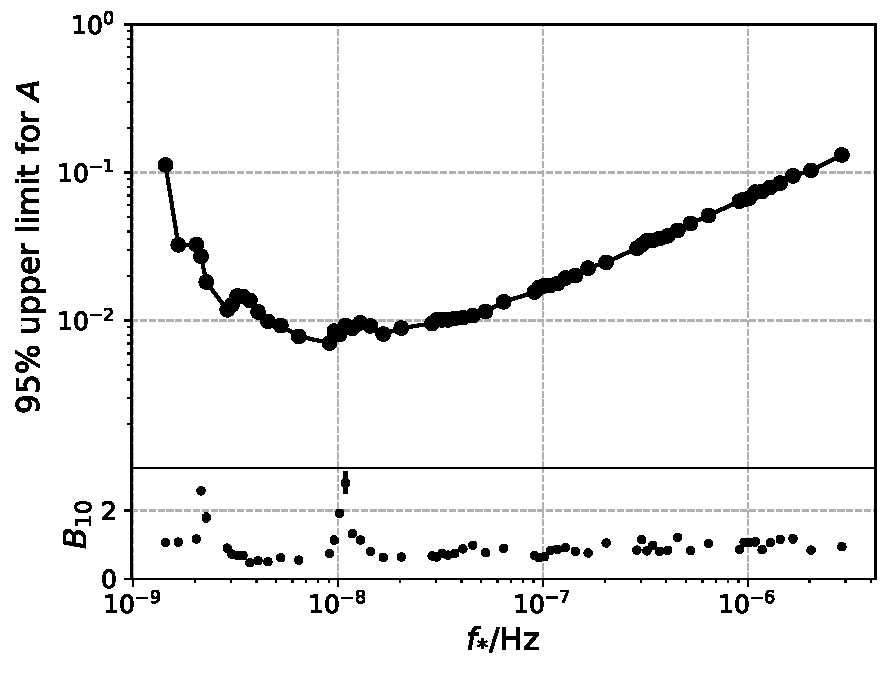
\includegraphics[width=0.8\textwidth]{A_upper.pdf}
    \bicaption{\label{A_upper} \textbf{上图}:NANOGrav 11年数据集中,曲率扰动功率谱振幅$A$的$95\%$上限与峰值频率$\fstar$的关系。\textbf{下图}:相应的贝叶斯因子$B_{10}$与峰值频率$\fstar$的关系。
    }{\textbf{Top panel}: the $95\%$ upper limits on the
        power spectrum amplitude $A$ of curvature perturbation as a function
        of the peak frequency $\fstar$ from the NANOGrav 11-year data set.
        \textbf{Bottom panel}: the corresponding Bayes factors $B_{10}$ as a
        function of the peak frequency $\fstar$.}
\end{figure}

\begin{figure}[h!]
    \centering
    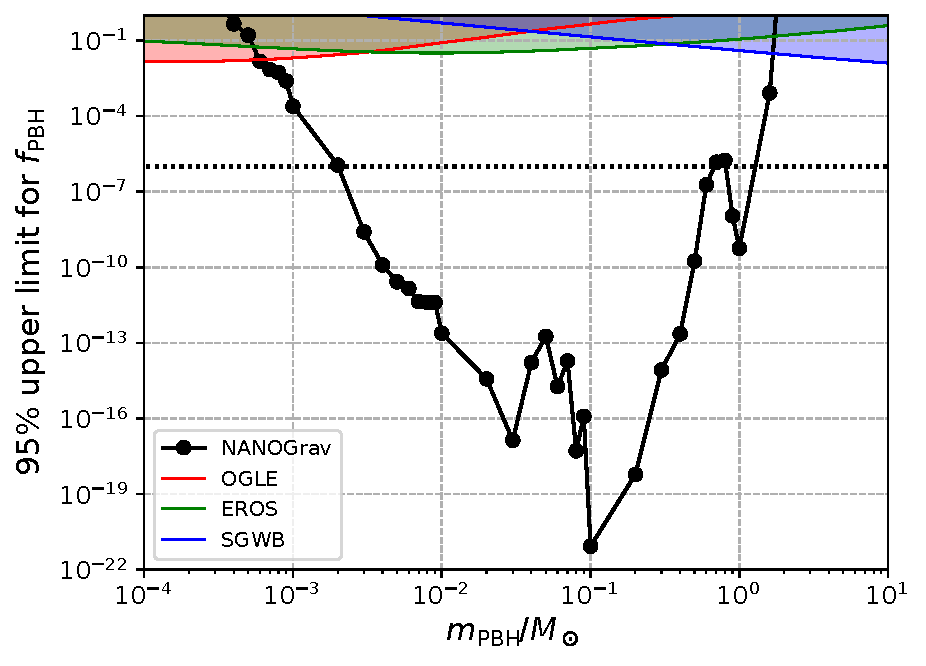
\includegraphics[width=0.8\textwidth]{fpbh_upper.pdf}
    \bicaption[从NANOGrav 11年数据集中得到的原初黑洞占冷暗物质丰度$\fpbh$的$95\%$上限关于原初黑洞质量$m_{\rm{PBH}}$的函数。图中还显示了来自OGLE微透镜(OGLE)、EROS/MACHO微透镜(EROS)和随机引力波背景的结果。水平虚线对应的是$10^{-6}$。]{\label{fpbh_upper} 从NANOGrav 11年数据集中得到的原初黑洞占冷暗物质丰度$\fpbh$的$95\%$上限关于原初黑洞质量$m_{\rm{PBH}}$的函数。图中还显示了来自OGLE微透镜(OGLE)\cite{Niikura:2019kqi}、EROS/MACHO微透镜(EROS)\cite{Tisserand:2006zx}和随机引力波背景\cite{Chen:2019irf}的结果。水平虚线对应的是$10^{-6}$。}{The $95\%$ upper limits on the abundance of primordial black holes
        in cold dark matter $\fpbh$ as a function of the primordial black hole mass $m_{\rm{PBH}}$ from the
        NANOGrav 11-year data set. 
        Results from OGLE microlensing (OGLE) \cite{Niikura:2019kqi},
        EROS/MACHO microlensing (EROS) \cite{Tisserand:2006zx}, 
        and SGWB \cite{Chen:2019irf} are also shown. 
        The horizontal dotted line corresponds to $10^{-6}$.}
\end{figure}

\Fig{A_upper}给出了从NANOGrav 11年数据集得到的功率谱振幅$A$的$95\%$置信上限和贝叶斯因子作为峰值频率$\fstar$的关系。尽管贝叶斯因子分布中有两个峰值,但两个峰值值都小于$3$,这意味着数据中信号的存在是``不值一提"的 \cite{BF}。由于每个峰值频率的贝叶斯系数$B_{10}$小于$3$,说明数据中与只含有噪声是一致的。\Fig{fpbh_upper}给出了原初黑洞在暗物质中的丰度$\fpbh$的$95\%$的置信度上限作为原初黑洞质量$m_{\rm{PBH}}$的关系。\Eq{mkrelation}给出了$m_{\rm{PBH}}$与$\fstar$的关系,而\Eq{fpbh}给出了$\fpbh$与$A$的关系。我们的结果意味着当前的PTA数据集已经能够通过标量诱导引力波对原初黑洞的丰度进行严格的限制。由\Fig{fpbh_upper}可知,在$[2\times 10^{-3}, 7\times 10^{-1}] \Msun$的质量范围内,原初黑洞的丰度小于$10^{-6}$。


我们首次在NANOGrav 11年数据集中搜索伴随着原初黑洞形成而不可避免产生的标量诱导力波的信号。由于没有发现显著的信号,我们对峰值频率范围$[1.5\times 10^{-9}, 3\times 10^{-6}]$Hz和质量范围$[4\times10^{-4}, 1.7]\Msun$的原初黑洞的丰度给出了$95\%$的上限。特别是,原初黑洞在$[2 \times 10^{-3}, 7\times 10^{-1}] M_\odot$ 质量范围内的丰度小于$10^{-6}$,这比已有文献中对这个质量范围的观测限制都要好得多。虽然我们假设原初黑洞的质量函数是单色的,但对于具有扩展质量分布的情况,标量诱导引力波的振幅也大致由标量功率谱的峰值振幅决定,因此从NANOGrav 11年数据中应该可以获得类似的对标量功率谱峰值振幅的约束。因此,也可以预期具有扩展质量分布的原初黑洞的丰度也会受到严格的限制。原则上,对具有扩展质量分布的情况的精确分析是模型依赖的。我们将在未来考虑原初黑洞有质量分布的情况。

%The constraint covers a wide 原初黑洞 mass window from $10^{-4}M_{\odot}$ to solar-mass window. At the most frequency band, corresponding to the subsolar-mass window $\sim0.1M_\odot$, the upper limit reach $\sim10^{-38}$. 

%Also, it is as expected that bringing the third-order correction into consideration leads to a several orders of magnitude difference $f_{\rm{pbh}}$. This is because $f_{\rm{pbh}}$ is very sensitive to $A$. It can be estimated from Eq.~(\ref{beta}) that
%\e
%\Delta f_{\rm{pbh}}= \frac{\zeta_c(\zeta_c-3A)}{6\sqrt{6\pi}A^{3}}\exp\(-{\zeta_c\over 2A}\)\Delta A.
%\q
%The third-order correction would lead to about a $10\%$ increase of the amplitude $\Delta A\approx0.1$. For a typical value $A=0.01$, the relative correction of the abundance would be $\Delta f_{\rm{pbh}}/f_{\rm{pbh}}\approx500$, rendering the higer-order corrections of the 标量诱导引力波 are indispensable.



%\begin{figure}[htbp!]
%\centering
%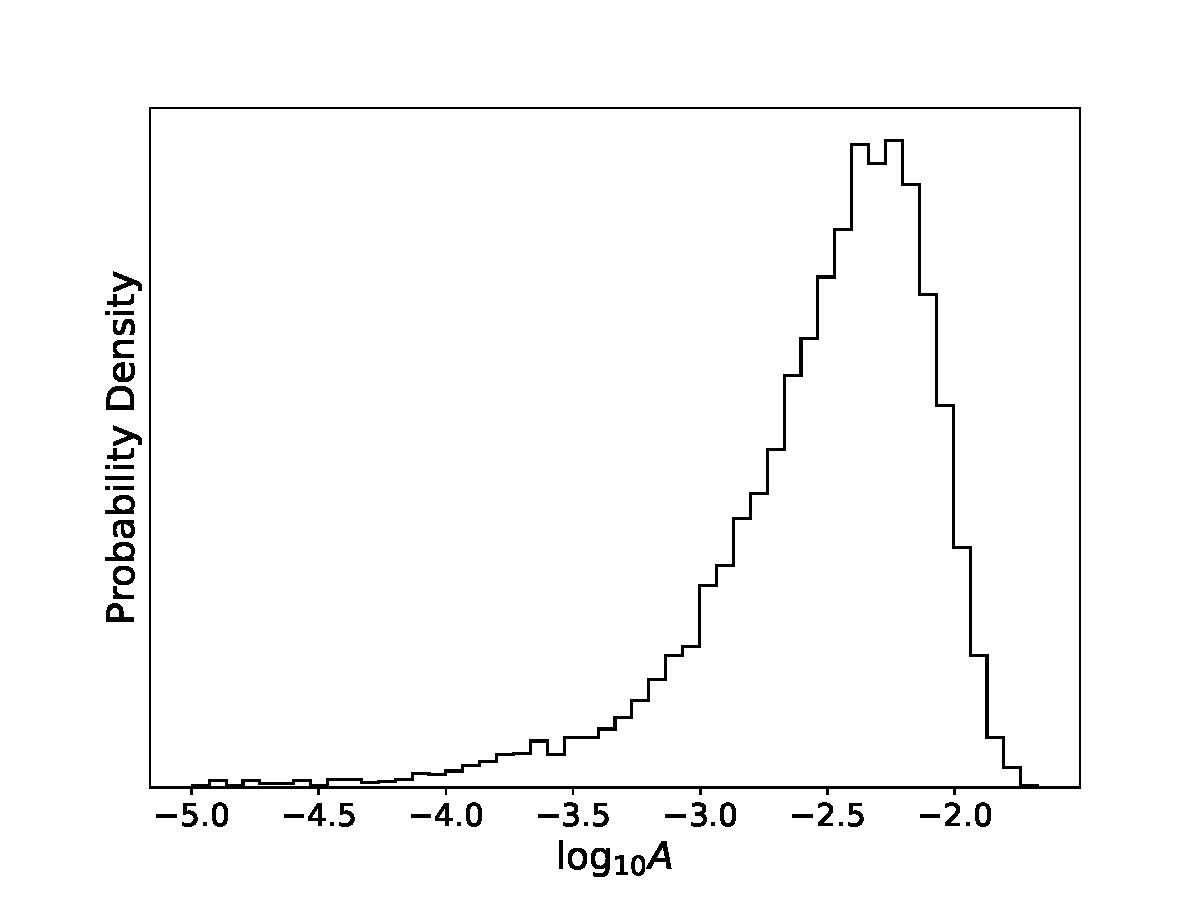
\includegraphics[width=0.8\textwidth]{A_post.pdf}
%\bicaption{当峰值频率为$\fstar=\rm{yr}^{-1}$时,曲率扰动幅度$A$的后验分布。 
%}{The posterior distribution of curvature perturbation
%amplitude $A$ when peak frequency $\fstar=\rm{yr}^{-1}$.}
%\label{A_post} 
%\end{figure}
%
%\begin{figure}
%\subfloat{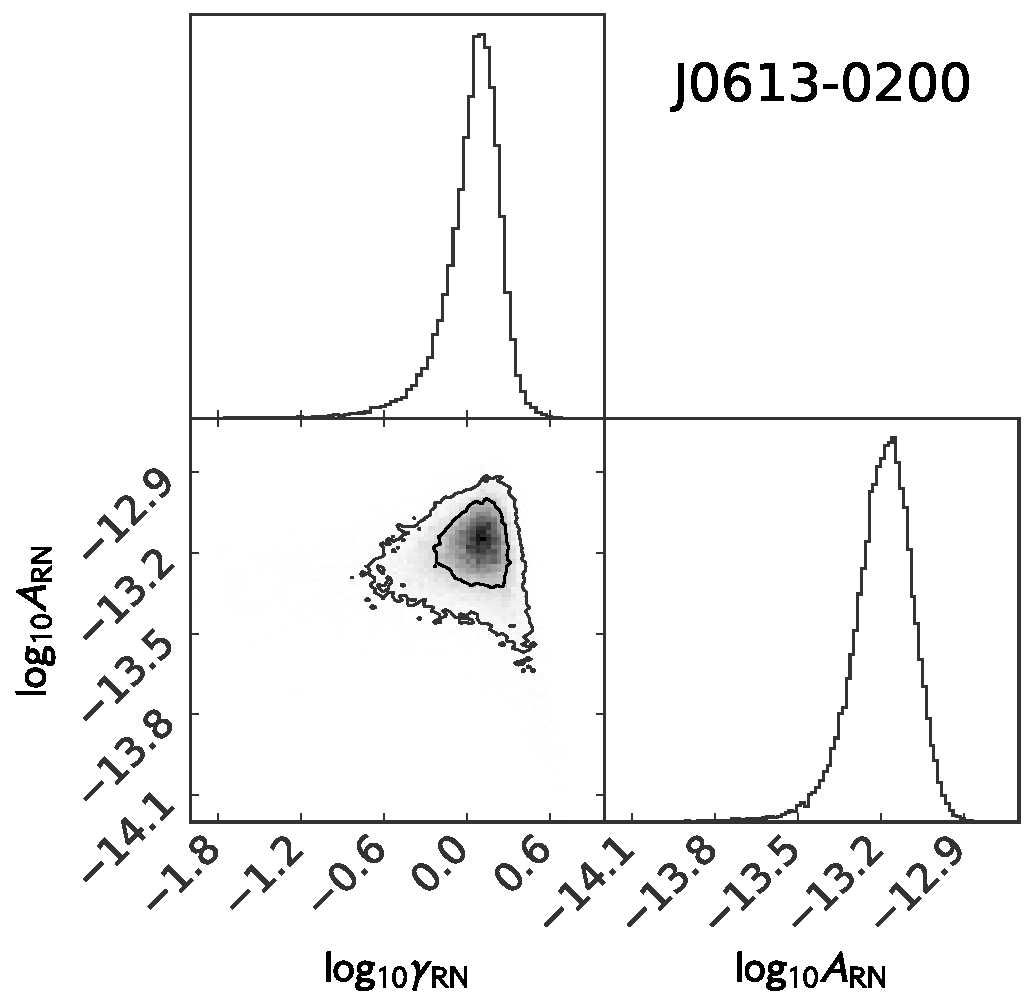
\includegraphics[width=0.45\textwidth]{J0613-0200.pdf}}\hspace{5mm} 
%\subfloat{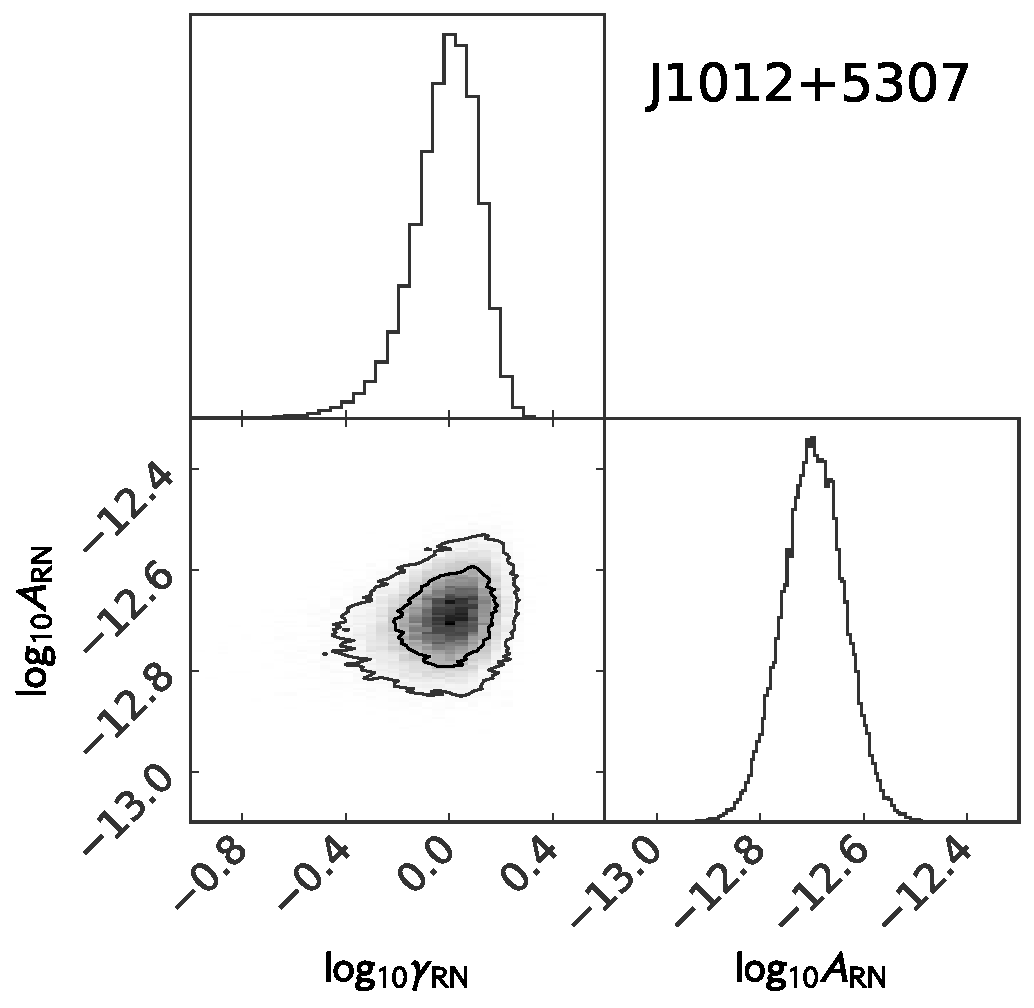
\includegraphics[width=0.45\textwidth]{J1012+5307.pdf}}\\
%\subfloat{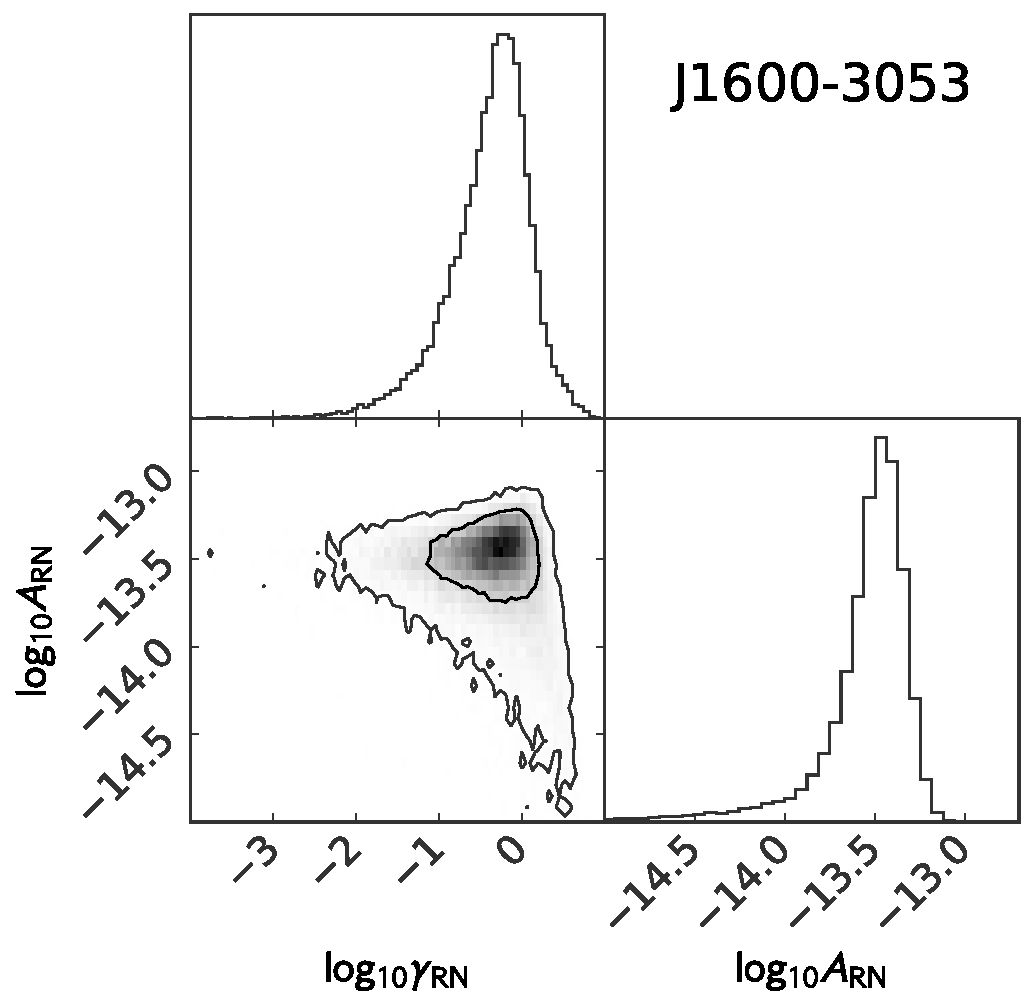
\includegraphics[width=0.45\textwidth]{J1600-3053.pdf}}\hspace{5mm} 
%\subfloat{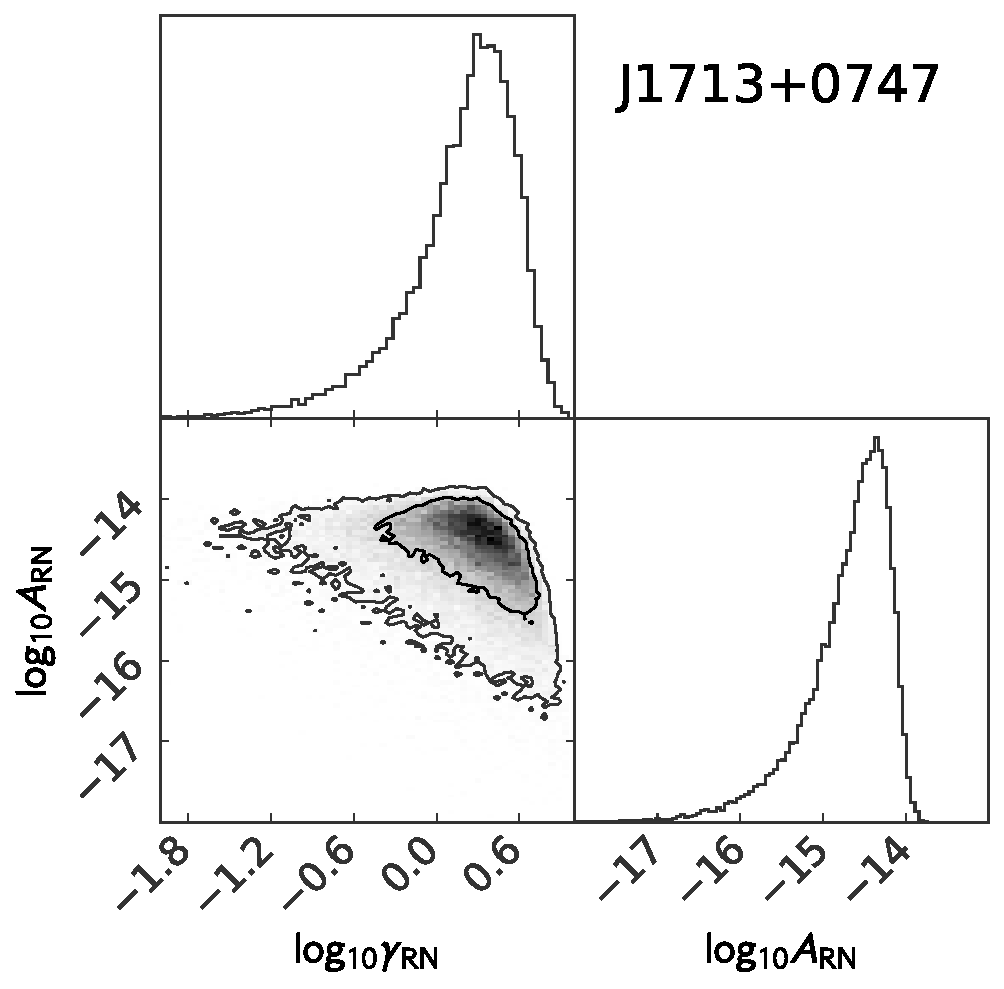
\includegraphics[width=0.45\textwidth]{J1713+0747.pdf}}\\
%\subfloat{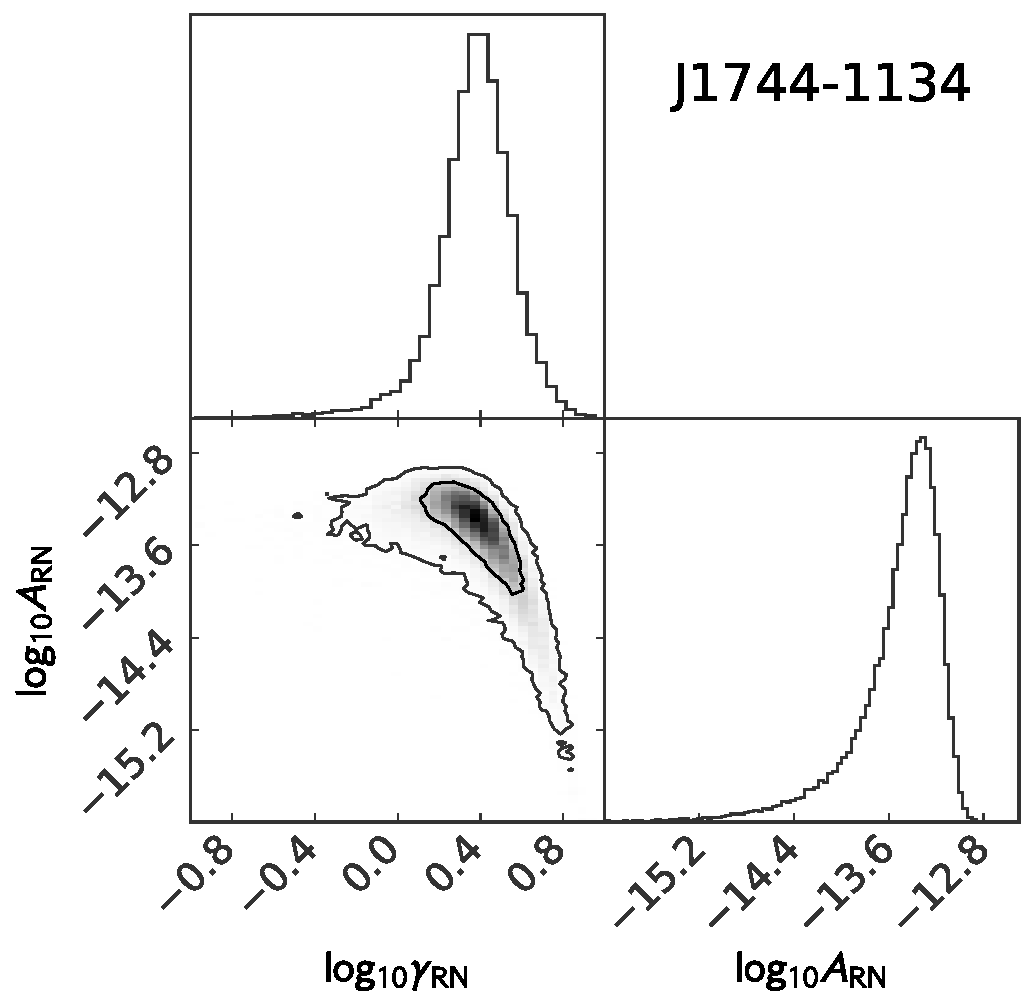
\includegraphics[width=0.45\textwidth]{J1744-1134.pdf}}\hspace{5mm} 
%\subfloat{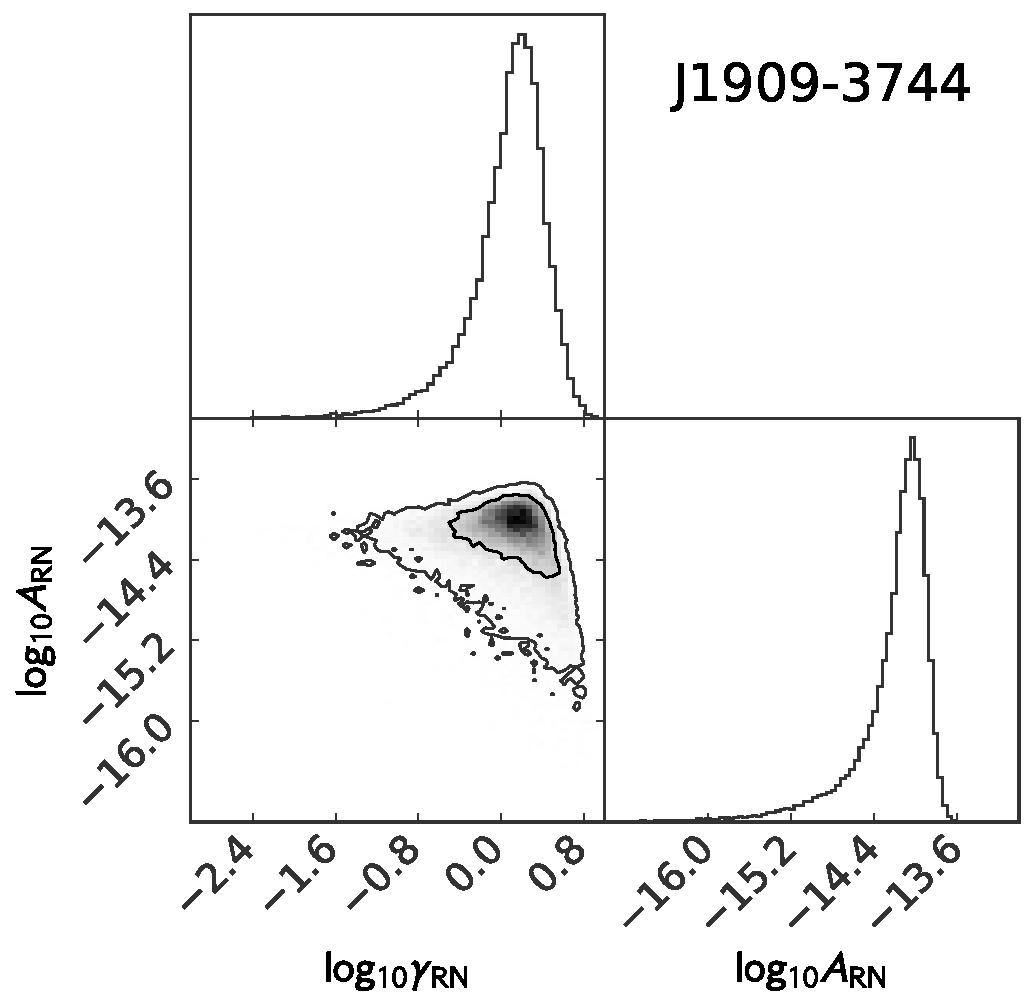
\includegraphics[width=0.45\textwidth]{J1909-3744.pdf}}
%\bicaption{当峰值频率$\fstar=\rm{yr}^{-1}$时,我们分析中使用的6颗脉冲星(见\Table{pulsars})的红噪声振幅$\ARN$和光谱指数$\gRN$的一维和二维边际化后验分布。每个子图给出了在$68\%$和$95\%$的置信度等值线。
%}{The one- and two-dimensional marginalized posterior distributions of the red-noise amplitude $\ARN$ and spectral index $\gRN$ for the $6$ pulsars
%(see \Table{pulsars}) used in our analysis when peak frequency
%$\fstar=\rm{yr}^{-1}$. 
%For each sub-figure, the contours are at $68\%$ and $95\%$ confidence levels
%respectively. }
%\label{psrs_post}
%\end{figure}

%However, the constraint given by this paper strongly depends on the assumption that the comoving curvature perturbations obey Gaussian statistics. This is because 原初黑洞 are supposed to form from the tail of the probability density function, so that the possibility to form a 原初黑洞 is extremely sensitive to non-Gaussianity \cite{Young:2018lec}. It has been studied in \cite{Cai:2018dig,Cai:2019amo,Cai:2019elf} that non-Gaussianity may intensely suppress the amplitude of the 标量诱导引力波 so that the null detection of 标量诱导引力波 may be given rise to large primordial non-Gaussianity.
\chapter{总结}

本文探索通过引力波来探测原初黑洞。首先,考虑所有其他原初黑洞以及线性密度扰动产生的力矩对原初双黑洞演化的影响,我们计算了具有一般质量分布情况下的原初双黑洞的并合率分布。利用我们得到的并合率分布以及\lvc 探测到的双黑洞并合的引力波数据,我们对原初黑洞占冷暗物质的丰度给出的限制为$10^{-3} \lesssim \fpbh \lesssim 10^{-2}$,证实了绝大多数的冷暗物质不是由恒星级质量的原初黑洞构成的。

其次,我们计算了双黑洞和双中子星并合产生的随机引力波背景。我们考虑了两种不同的双黑洞形成机制,分别是天体物理双黑洞和原初双黑洞机制。并分析这一引力波背景能否被未来的引力波探测器(比如LISA)观测到。我们发现双黑洞和双中子星产生的随机引力波背景可以被未来的空间引力波探测器LISA探测到。如果这一引力波背景没能从LISA探测器中扣除掉,将会构成LISA的额外噪音,从而降低LISA的探测能力。

然后,我们探讨了通过下一代地面引力波探测器,比如ET和CE,来区分原初黑洞和天体物理黑洞的可能性。通过定向搜寻亚太阳质量的双黑洞系统,我们估算了原初黑洞占暗物质丰度的可探测下限。另外,我们预测了ET和CE能够探测到的双黑洞事件数目随红移的分布,从而来区分原初黑洞和天体物理黑洞模型。

最后,我们首次在NANOGrav 11年的脉冲星计时阵列数据集中搜索伴随原初黑洞形成而产生的标量诱导引力波信号。由于没有发现统计意义上显著的引力波信号,我们对质量在$[2 \times 10^{-3}, 7\times 10^{-1}]$太阳质量区间的原初黑洞占冷暗物质的丰度给出了迄今为止最严格的限制。


%-
%-> Appendix
%-
\cleardoublepage%
\appendix% initialize the environment
%\chapter{中国科学院大学学位论文撰写要求}% appendix content
%-
%-> Backmatter: bibliography, glossary, index
%-
\backmatter% initialize the environment
\intotoc*{\cleardoublepage}{\bibname}% add link to toc
\artxifstreq{\artxbib}{bibtex}{% enable bibtex
    \bibliography{Biblio/ref}% bibliography
}{%
    \printbibliography% bibliography
}
%---------------------------------------------------------------------------%
%->> Backmatter
%---------------------------------------------------------------------------%
\chapter[致谢]{致\quad 谢}\chaptermark{致\quad 谢}% syntax:
转瞬之间,我已在理论所学习了四年。临别之际,我想对所有关心和帮助过我的人表示最衷心的感谢!

我要真诚感谢我的导师黄庆国研究员对我的悉心栽培!黄老师在科研和生活方面都给予我极大的帮助。在科研方面,黄老师对物理学的前沿有敏锐的洞察力,从入学的时候就建议我从事引力波和原初黑洞这一新兴领域的研究工作。黄老师的物理图像清晰,我时常能从他那里获得关于物理现象的新见解。在我科研工作遇到问题的时候,黄老师总能一针见血地指明问题的关键,使得我们能够专心攻克难点,取得进展。黄老师在科研工作上具有极大的激情,他似乎无时无刻不在思考物理问题,并总能提出很多奇思妙想并乐意与我们分享。在科研遇到困难的时候,我总能随时通过各种通信工具向他求助和探讨。记得有多次为了尽快完成手上的科研工作,黄老师不惜牺牲休息的时间,与我们通过微信或小鱼易连讨论至深夜甚至凌晨。这种激情一直激励着我不断努力工作。在黄老师的指导下做研究是愉快和高效的。在生活方面,黄老师给了我诸多照顾。在我博士入学之前的半年,黄老师就提前资助我来理论所访问。读博后,黄老师还多次资助我去国内外参加各种学术交流活动,并经常给我推荐就业信息。在读博期间,我还经常向黄老师请假回家与家人团聚,黄老师每次都通情达理地批准了。我再次向黄老师表示最诚挚的谢意!

我要感谢我的合作者们。他们是黄庆国老师、Vivien Raymond老师、戚虹老师和林文斌老师,以及袁晨师弟、黄帆师弟、李君师姐、罗华美学妹和吴玉梅师妹。特别是袁晨师弟,他思维活跃、物理图像清晰,我们的合作是卓有成效的,已经完成了5篇文章。


我要感谢台湾师范大学的林丰利老师以及广州大学的张靖仪老师,他们曾分别邀请和资助我去访问。此外,我还要感谢理论所提供的平台,让我有机会申请到国科大的资助,从而能够在英国卡迪夫大学进行为期一年的访问学习。为此,我要感谢黄庆国老师、刘润球老师和戚虹老师在我申请访学过程中提供的无私帮助。我要感谢在卡迪夫大学访学时的导师戚虹老师和Vivien Raymond老师,他们总能在百忙之中抽空听取我的科研进展并讨论和指导下一步工作。我还要感谢Edward Fauchon-Jones、Sebastian Khan和Jonathan E. Thompson,他们在我访学期间为我解答了关于中子星黑洞模板的各种问题。我要感谢Charlie Hoy、Virginia d'Emilio和Cecilio García-Quirós,他们曾帮我解答关于\texttt{Bilby}和\texttt{PESummary}软件包的各种问题。

我要感谢组内的同学们。王赛师兄、皮石师兄、程程师姐、张克超师兄、邢宇航师兄、王科师兄、陈璐师姐、李君师姐、桑语师兄、张雪师姐、方芸、黄帆、袁晨、吴玉梅、郭忠凯、孟德双、国荣祯和韩雨轩在平时的学习生活中,为我提供了不少帮助。

我要感谢国内的室友戴卫明学长、柳浪和贾乙丁提供了良好的宿舍环境,使我得以安心学习和科研。我要感谢在英国访学期间的室友杜慕皓、王凯和孙佳时常分享他们的美食,以及在我心情低落的时候给予我诸般安慰;怀念在疫情期间一起斗地主的欢乐时光。

我要感谢在理论所行政岗位上默默付出的王丽老师、孙亚宁老师、郭舒婷老师和石平老师。特别是石平老师曾多次主动提醒和联系我完成一些行政上的事务。

我要感谢我的硕士导师韦浩教授。韦老师不仅手把手地引导我进入科研领域,还在我读博期间时常关心我的动态。

我要感谢我的家人们对我的理解、包容和支持。感谢父母几十年来的养育之恩!感谢岳父母对我妻子和孩子的照顾!感谢妻子对我的支持!

我要感谢上帝在我人生每个阶段的带领。我要感谢教会的众弟兄姊妹们,是你们让我不管是身处国内还是异国他乡都能感受到上帝的爱。

谨以此文献给我的儿子陈曦。


\chapter{作者简历及攻读学位期间发表的学术论文与研究成果}

\section*{作者简历:}

2008年9月至2012年6月,在福州大学紫金矿业学院获学士学位。

2012年9月至2015年3月,在北京理工大学物理学院获硕士学位。

2015年9月至2016年10月,在湖南文理学院任教师。

2019年10月至2020年10月,在英国卡迪夫大学物理与天文系访学(加入LIGO)。

2017年9月至2021年6月,在中国科学院理论物理研究所攻读博士学位。

\section*{短作者文章:}
\begin{enumerate}
    \item \href{https://arxiv.org/abs/2101.06869}{Non-tensorial Gravitational Wave Background in NANOGrav 12.5-Year Data Set}\\ \href{https://arxiv.org/abs/2101.06869}{arXiv:2101.06869 [astro-ph.CO]}\\
    \textbf{Zu-Cheng Chen}, Chen Yuan, Qing-Guo Huang
    
    \item \href{https://journals.aps.org/prd/abstract/10.1103/PhysRevD.101.063018}{Scalar induced gravitational waves in different gauges}\\
    Physical Review D, 2020, 101(6): 063018, \href{https://arxiv.org/abs/1912.00885}{arXiv:1912.00885 [astro-ph.CO]}\\
    Chen Yuan, \textbf{Zu-Cheng Chen}, Qing-Guo Huang
    
    \item \href{https://link.springer.com/article/10.1007\%2Fs11467-019-0936-x}{Extraction of gravitational wave signals with optimized convolutional neural network}\\
    Frontiers of Physics, 2020, 15(1): 14601\\
    Hua-Mei Luo, Wenbin Lin, \textbf{Zu-Cheng Chen}, Qing-Guo Huang    
    
    \item \href{https://journals.aps.org/prl/abstract/10.1103/PhysRevLett.124.251101}{Pulsar Timing Array Constraints on Primordial Black Holes with NANOGrav 11-Year Dataset}\\
    Physical Review Letters, 2020, 124(25): 251101, \href{https://arxiv.org/abs/1910.12239}{arXiv:1910.12239 [astro-ph.CO]}\\    
    \textbf{Zu-Cheng Chen}, Chen Yuan, Qing-Guo Huang    
    
    \item \href{https://journals.aps.org/prd/abstract/10.1103/PhysRevD.101.043019}{Log-dependent slope of scalar induced gravitational waves in the infrared regions}\\
    Physical Review D, 2020, 101(4): 043019, \href{https://arxiv.org/abs/1910.09099}{arXiv:1910.09099 [astro-ph.CO]}\\ 
    Chen Yuan, \textbf{Zu-Cheng Chen}, Qing-Guo Huang
    
    \item \href{https://link.springer.com/article/10.1007/s11433-019-9605-5}{Measuring the tilt of primordial gravitational-wave power spectrum from observations}\\
    Science China (Physics, Mechanics \& Astronomy), 2019 (11): 16, \href{https://arxiv.org/abs/1907.09794}{arXiv:1907.09794 [astro-ph.CO]}\\
    Jun Li, \textbf{Zu-Cheng Chen}, Qing-Guo Huang
    
    \item \href{https://journals.aps.org/prd/abstract/10.1103/PhysRevD.100.081301}{Probing primordial-black-hole dark matter with scalar induced gravitational waves}\\
    Physical Review D, 2019, 100(8): 081301, \href{https://arxiv.org/abs/1906.11549}{arXiv:1906.11549 [astro-ph.CO]}\\
    Chen Yuan, \textbf{Zu-Cheng Chen}, Qing-Guo Huang
    
    \item \href{https://iopscience.iop.org/article/10.1088/1475-7516/2020/08/039}{Distinguishing Primordial Black Holes from Astrophysical Black Holes by Einstein Telescope and Cosmic Explorer}\\
    Journal of Cosmology and Astroparticle Physics, 2020, 2020(08): 039, \href{https://arxiv.org/abs/1904.02396}{arXiv:1904.02396 [astro-ph.CO]}\\
    \textbf{Zu-Cheng Chen},Qing-Guo Huang
    
    \item \href{https://iopscience.iop.org/article/10.3847/1538-4357/aaf581}{Stochastic Gravitational-Wave Background from Binary Black Holes and Binary Neutron Stars and Implications for LISA}\\
    The Astrophysical Journal, 2019, 871(1): 97, \href{https://arxiv.org/abs/1809.10360}{arXiv:1809.10360 [gr-qc]}\\
    \textbf{Zu-Cheng Chen}, Fan Huang, Qing-Guo Huang
    
    \item \href{https://iopscience.iop.org/article/10.3847/1538-4357/aad6e2}{Merger Rate Distribution of Primordial-Black-Hole Binaries}\\
    The Astrophysical Journal, 2018, 864(1): 61, \href{https://arxiv.org/abs/1801.10327}{arXiv:1801.10327 [astro-ph.CO]}\\
    \textbf{Zu-Cheng Chen},Qing-Guo Huang
\end{enumerate} 

\section*{长作者文章:}
\begin{enumerate}
    
    \item \href{https://arxiv.org/abs/2103.08520}{Search for anisotropic gravitational-wave backgrounds using data from Advanced LIGO's and Advanced Virgo's first three observing runs}\\ \href{https://arxiv.org/abs/2103.08520}{arXiv:2103.08520 [gr-qc]}\\
    LIGO Scientific and Virgo and KAGRA Collaborations
    
    \item \href{https://arxiv.org/abs/2101.12248}{Constraints on cosmic strings using data from the third Advanced LIGO-Virgo observing run}\\ \href{https://arxiv.org/abs/2101.12248}{arXiv:2101.12248 [gr-qc]}\\
    LIGO Scientific and Virgo and KAGRA Collaborations

    \item \href{https://arxiv.org/abs/2101.12130}{Upper Limits on the Isotropic Gravitational-Wave Background from Advanced LIGO's and Advanced Virgo's Third Observing Run}\\ \href{https://arxiv.org/abs/2101.12130}{arXiv:2101.12130 [gr-qc]}\\
    LIGO Scientific and Virgo and KAGRA Collaborations    
    
    \item \href{https://arxiv.org/abs/2012.12926}{Diving below the spin-down limit: Constraints on gravitational waves from the energetic young pulsar PSR J0537-6910}\\ \href{https://arxiv.org/abs/2012.12926}{arXiv:2012.12926 [astro-ph.HE]}\\
    LIGO Scientific and Virgo and KAGRA Collaborations      
    
    \item \href{https://journals.aps.org/prd/abstract/10.1103/PhysRevD.103.064017}{All-sky search in early O3 LIGO data for continuous gravitational-wave signals from unknown neutron stars in binary systems}\\     
    Physical Review D, 2021, 103(6): 064017, \href{https://arxiv.org/abs/2012.12128}{arXiv:2012.12128 [gr-qc]}\\
    LIGO Scientific and Virgo and KAGRA Collaborations    
\end{enumerate}


\section*{获奖情况:}
\begin{itemize}
    \item 2020-2021学年中国科学院大学三好学生标兵
    
    \item 2020年理论物理研究所曙光优秀奖
    
    \item 2019年博士研究生国家奖学金
    
    \item 2018-2019学年中国科学院大学三好学生
    
    \item 2018年理论物理研究所曙光特别奖
    
    \item 2012年硕士研究生国家奖学金
    
\end{itemize}



%\chapter[目录]{标题}\chaptermark{页眉}
\thispagestyle{noheaderstyle}% 如果需要移除当前页的页眉
%\pagestyle{noheaderstyle}% 如果需要移除整章的页眉



\cleardoublepage[plain]% 让文档总是结束于偶数页,可根据需要设定页眉页脚样式,如 [noheaderstyle]
%---------------------------------------------------------------------------%
% other information
\end{document}
%---------------------------------------------------------------------------%

